% Copyright (C) 2020  George P. W. Williams, Jr.

\documentclass[11pt,letterpaper]{report}

\usepackage{sphack}		% six wierd spacing around commands (like \index) that should be invisible
\usepackage{path}		% for control line-breaking in file paths, etc
	% The following lists where discretionary breaks are allowed in \path
	% default: \discretionaries |~!@$%^&*()_+`-=#{"}[]:;'<>,.?\/|
	\discretionaries |_&+-=.\/|		%% must have a "\" before "/" in the pattern
\usepackage{graphicx}	% add support for including graphics files
\graphicspath{{figs/}}
\usepackage[backend=bibtex,style=alphabetic,sorting=nyt]{biblatex}
\addbibresource{geco}


\newtoggle{hyperlinks}
% use one of the two following lines
\toggletrue{hyperlinks}	% add hyperlinks in the pdf
%\togglefalse{hyperlinks}	% do NOT add hyperlinks

% !!! whenever changing between using/not using hyperref, rebuild the index
% !!! assure that the \usepackage{path} line precedes all this

\iftoggle{hyperlinks}{%
	% add hyperlinks in PdfLatex for things where it would be convenient
	\usepackage{hyperref}
}{
	% if not using hyperref, define a substitute for \href:
	\def\href#1#2{\path|#1|}
}


\def\gecoversion{$2.1.2$}

\title{GECO: A CLOS-based Framework for\\ Prototyping Genetic Algorithms
	\vskip \medskipamount%
	\normalsize --- Version \gecoversion{} ---}
	\author{George P. W. Williams, Jr.\\
	\normalsize\tt george.p.williams@pobox.com}

%
%  File:	ITALIC.TEX
%
%  Author:	Hunter Goatley
%		goathunter@goatley.com
%
%  Date:	August 21, 1991
%
%  Abstract:
%
%	The macros \ital and \slant are defined to typeset tex in italic
%	(\it) and slanted (\sl) fonts, automatically inserting the italic
%	correction (\/) if necessary.  The correction is not inserted if
%	the token following the parameter is a period or a comma, as
%	suggested on page 14 of _The TeXbook_.
%
%	Based on the \predict macro presented in _TeX for the Impatient_,
%	p. 233.
%
%	These macros use \toks0 as a temporary.
%
%	The \futurelet\it@next in \ital and \slant defines \it@next to be
%	whatever the character following the parameter is.  \d@slant checks
%	to see if \it@next is a comma or period; if it is neither, the
%	italic correction (\/) is included.
%
\catcode`\@=11				% Temporarily make @ a letter
\def\ital#1{\toks0={#1}\let\slf@nt=\it\futurelet\it@next\d@slant}
\def\slant#1{\toks0={#1}\let\slf@nt=\sl\futurelet\it@next\d@slant}
\def\d@slant{{\slf@nt\the\toks0}%
	\ifx\it@next,%			% If \it@next is not a comma
	\else\ifx\it@next.%		% ... and is not a period
	\else\/%			% ... insert the correction (\/)
	\fi\fi%				% ...
	\let\it@next=\relax%		% "Undefine" \it@next
	}
\catcode`\@=12				% Reset @ as other
		%%%% \import{/usr/local/texlive/2020/texmf-dist/doc/plain/newsletr/}{italic.tex} %% doesn't work

% Copyright (C) 2020  George P. W. Williams, Jr.
% Page style parameters
\addtolength{\oddsidemargin}{-.5in}
\addtolength{\evensidemargin}{-.5in}
\addtolength{\textwidth}{1in}
\addtolength{\topmargin}{-.5in}
\addtolength{\textheight}{1.0in}
\setlength{\headheight}{20pt}
\setlength{\headsep}{20pt}
\raggedbottom
\clubpenalty=8000 \widowpenalty=8000 % I hate orphans & widows

\makeatletter  %force abstract to appear on the same page as the title
	\def\titlepage{\@restonecolfalse\thispagestyle{empty}\c@page\z@}
	\def\endtitlepage{}
\makeatother

% Section numbering & TOC style parameters
\setcounter{secnumdepth}{4}
\setcounter{tocdepth}{3}

% Paragraph style parameters
\setlength{\parindent}{0pt}
\setlength{\parskip}{1.5ex}
\newskip  \normalparskip        
\normalparskip = 1.5ex

%\tracingall

%%
%% Basic macros
%%

	\makeatletter	% allow @-sign to be considered as a letter; for special definitions

%%% The following \cl macros are based on a version lifted from the CLIM 2 spec.
%% This allows hyphenation of CL symbols at the hyphens that exist in
%% the symbol name, but noplace else, e.g., \cl{standard-region-union}.
%% Hyphens are active characters, so we don't break Tags Search.
%% This version of \cl has additional smarts to allow TeX's special characters
%% (except braces and "\"), based on LaTeX's verbatim.
%% When you supply a default value for optional or keyword arguments,
%% use this idiom:  \key (filled \cl{t})

% The \doclspecials is a modified version of \dospecials from plain.tex
\def\doclspecials{\do\$\do\&\do\#\do\^\do\_\do\%\do\~}
% (not counting ascii null, tab, linefeed, formfeed, return, delete).
% For \cl we also removed the space, \, {, }, ^^A, and ^^K.
% Each symbol in the list is preceded by \do, which can be defined
% if you want to do something to every item in the list.

% The clhyphen definitions are necessary to support the automatic cl indexing macros.
% \index does strange things to its args, and the hyphen mustn't get expanded.
\def\cl@normalhyphen{-}
\def\cl@breakinghyphen{{\tt \char`\-}\penalty\exhyphenpenalty}
\def\cl@hyphen{\cl@normalhyphen}
\def\setclnormalhyphen{\let\cl@hyphen=\cl@normalhyphen}
\def\setclbreakinghyphen{\let\cl@hyphen=\cl@breakinghyphen}

{\catcode`\-=\active%
\gdef\setclspecials{\catcode``=\active\@noligs\frenchspacing\@vobeyspaces%
\setclbreakinghyphen\catcode`\-=\active\def-{\cl@hyphen}\def\\{\char`\\}%
\let\do=\@makeother\doclspecials}
\gdef\arg{\begingroup\setclspecials%
\def-{{\sl\char`\-}\penalty\exhyphenpenalty}%
\@xarg}}
\def\@xarg#1{{\sl#1}\endgroup}
\def\cl{\begingroup\setclspecials\@xcl}
\def\@xcl#1{{\tt#1}\endgroup}

%%% \begin{\clcode} ... \end{clcode} environment, based on LaTeX's verbatim.
\usepackage{code-os}
\def\clcode{\codeaux{}}
\let\endclcode=\endcodeaux

\def\ttdash{\mbox{{\tt -}}}	%for use in math mode

%\begingroup
%  \catcode`|=0 \catcode`[= 1 \catcode`]=2 \catcode`\{=12 \catcode`\}=12 \catcode`\\=12
%  |gdef|@xclcode#1\end{clcode}[#1|end[clcode]]
%|endgroup
%\def\clcode{\trivlist \item[]\if@minipage\else\vskip\parskip\fi
%  \leftskip\@totalleftmargin\rightskip\z@
%  \parindent\z@\parfillskip\@flushglue\parskip\z@
%  \@tempswafalse \def\par{\if@tempswa\hbox{}\fi\@tempswatrue\@@par}
%  \obeylines \tt \catcode``=\active \@noligs \frenchspacing\@vobeyspaces
%  \let\do=\@makeother \doclspecials \@xclcode}
%\let\endclcode=\endtrivlist

%%
%% Special indexing macros
%%

%\def\dowithonearg#1{\def\argone{#1}\do}
%\def\dowithtwoargs#1#2{\def\argone{#1}\def\argtwo{#2}\do}

%% inline references that are indexed

% singly indexed
% common lisp
\def\clinx{\begingroup\setclspecials\@xclinx}
	\def\@xclinx#1{\@xcl{#1}\@bsphack\setclnormalhyphen\index{{\tt#1}}\@esphack}

% ...d variants are doubly indexed
\def\cldinx{\begingroup\setclspecials\@xcldinx}
	\def\@xcldinx#1#2{\@xcl{#1}\ttdblinx{#1}{#2}}

	\def\ttdblinx#1#2{\@bsphack\begingroup\setclspecials\setclnormalhyphen%
	\index{{\tt#1}!#2}\index{#2!{\tt#1}}\endgroup\@esphack}

% macros, functions, ...
\def\inxmac{\begingroup\setclspecials\@xinxmac}
	\def\@xinxmac#1{\@xcldinx{#1}{Macro}}

\def\inxfun{\begingroup\setclspecials\@xinxfun}
	\def\@xinxfun#1{\@xcldinx{#1}{Function}}

\def\inxgeneric{\begingroup\setclspecials\@xinxgeneric}
	\def\@xinxgeneric#1{\@xcldinx{#1}{Generic Function}}

\def\inxmethod{\begingroup\setclspecials\@xinxmethod}
	\def\@xinxmethod#1{\@xcldinx{#1}{Primary Method}}

\def\inxbeforemethod{\begingroup\setclspecials\@xinxbeforemethod}
	\def\@xinxbeforemethod#1{\@xcldinx{#1}{:Before Method}}

\def\inxaftermethod{\begingroup\setclspecials\@xinxaftermethod}
	\def\@xinxaftermethod#1{\@xcldinx{#1}{:After Method}}

\def\inxaroundmethod{\begingroup\setclspecials\@xinxaroundmethod}
	\def\@xinxaroundmethod#1{\@xcldinx{#1}{:Around Method}}

\def\inxvar{\begingroup\setclspecials\@xinxvar}
	\def\@xinxvar#1{\@xcldinx{#1}{Variable}}

\def\inxconst{\begingroup\setclspecials\@xinxconst}
	\def\@xinxconst#1{\@xcldinx{#1}{Constant}}

\def\inxclass{\begingroup\setclspecials\@xinxclass}
	\def\@xinxclass#1{\@xcldinx{#1}{Class}}

\def\inxslot{\begingroup\setclspecials\@xinxslot}
	\def\@xinxslot#1{\@xcldinx{#1}{Slot}}

\def\inxinitarg{\begingroup\setclspecials\@xinxinitarg}
	\def\@xinxinitarg#1{\@xcldinx{#1}{Initarg}}

\def\inxtype{\begingroup\setclspecials\@xinxtype}
	\def\@xinxtype#1{\@xcldinx{#1}{Type}}

%%
%% Miscellaneous
%%


\long\def\issue#1#2{{\sl Issue: #2 ---~#1}}
\def\bold#1{{\bf #1}}  % italic.sty also defines \ital{} and \slant{}


% \comment<some-char>...text...<same-char> comments out TeX source
% analogous to \verb<some-char>...text...<same-char>
% sp. case: \comment{...text...} == \comment}...text...}
\def\comment{%   Stolen from slatex.sty
\begingroup \let\do\@makeother \dospecials \@comm}
\def\word@nd{\hskip-.35em\penalty\@M\null}
\begingroup\catcode`\<1\catcode`\>2
\catcode`\{12\catcode`\}12
\long\gdef\@comm#1<%
\if#1{\long\def\@tempa ##1}<\endgroup\word@nd>\else
	\long\def\@tempa ##1#1<\endgroup\word@nd>\fi
\@tempa>
\endgroup

%% Use \concept when you are introducing a term for the first time, and
%% want it in the index.  Use \term after that.
\def\concept#1{{\sf#1}\@bsphack\index{#1|ital}\@esphack}
\def\term#1{{\sf#1}}

	\makeatother	% reverses the effect of \makeatletter

%%
%% Definition types
%%

\def\removedepth{\ifdim \prevdepth>-1000pt \vskip -\prevdepth\fi}
\def\Vskip #1!{\endgraf\removedepth     
               \ifdim \lastskip<#1 \ifdim \lastskip>0pc
               \removelastskip\fi 
               \vskip#1\fi}

\def\outdent#1{\noindent\hbox to 0pc{\hskip -1.5pc #1\hss}\ignorespaces}
\def\brac#1{\rm[{\it #1\/}]}

%% Use these when you want to leave vertical whitespace above
\def\Dodoc#1#2{\Vskip \bigskipamount!%
	\outdent{$\Rightarrow$}\index{{\tt #1}!#2|ital}\index{#2!{\tt #1}|ital}%
	{\tt #1\hfill\hbox{\brac{\it #2\/}}%
		\Vskip .1pt!}}
\def\Dodocf#1#2#3{\Vskip \bigskipamount!%
	\outdent{$\Rightarrow$}\index{{\tt #1}!#3|ital}\index{#3!{\tt #1}|ital}%
	{\hangindent=1cm\hangafter=1%
		\tt #1\hfill\hbox{\brac{\it #3\/}}\linebreak%
		{\raggedright{\sl #2}\hfill\Vskip .1pt!}}}
%\def\Dodocv#1#2#3{\vbox spread -10pt {\Vskip \bigskipamount!%
\def\Dodocv#1#2#3{\vbox spread -2pt {\Vskip \bigskipamount!%
	\outdent{$\Rightarrow$}\index{{\tt #1}!#3|ital}\index{#3!{\tt #1}|ital}%
	{\hangindent=1cm\hangafter=1%
		\tt #1\hfill\hbox{\brac{\it #3\/}}\linebreak%
		{\raggedright{\tt #2}\hfill\Vskip .1pt!}}\vss}}

%% Use these when you want to leave some vertical whitespace above
\def\Defmacro #1 #2 {\Dodocf {#1} {#2} {Macro}}
\def\Defun #1 #2 {\Dodocf {#1} {#2} {Function}}
\def\Defgeneric #1 #2 {\Dodocf {#1} {#2} {Generic Function}}
\def\Defmethod #1 #2 {\Dodocf {#1} {#2} {Primary Method}}
\def\Defbeforemethod #1 #2 {\Dodocf {#1} {#2} {:Before Method}}
\def\Defaftermethod #1 #2 {\Dodocf {#1} {#2} {:After Method}}
\def\Defaroundmethod #1 #2 {\Dodocf {#1} {#2} {:Around Method}}
\def\Defvar #1 {\Dodoc {#1} {Variable}}
\def\Defvarv #1 #2 {\Dodocv {#1} {#2} {Variable}}
\def\Defconst #1 {\Dodoc {#1} {Constant}}
\def\Defconstv #1 #2 {\Dodocv {#1} {#2} {Constant}}
\def\Defclass #1 {\Dodoc {#1} {Class}}
\def\Defclassv #1 #2 {\Dodocf {#1} {#2} {Class}}
\def\Defslot #1 {\Dodoc {#1} {Slot}}
\def\Defslotv #1 #2 {\Dodocv {#1} {#2} {Slot}}
\def\Definitarg #1 {\Dodoc {#1} {Initarg}}
\def\Deftype #1 {\Dodoc {#1} {Type}}
\def\Defoption #1 {\Dodoc {#1} {Option}}
\def\Defcondition #1 {\Dodoc {#1} {Condition}}
\def\Defrestart #1 {\Dodoc {#1} {Restart}}

%% Use these when you don't want to leave any vertical whitespace above
\def\dodoc#1#2{\Vskip .1pt!%
	\outdent{$\Rightarrow$}\index{{\tt #1}!#2|ital}\index{#2!{\tt #1}|ital}%
	{\tt #1\hfill\hbox{\brac{\it #2\/}}%
		\Vskip .1pt!}}
\def\dodocf#1#2#3{\Vskip .1pt!%
	\outdent{$\Rightarrow$}\index{{\tt #1}!#3|ital}\index{#3!{\tt #1}|ital}%
	{\hangindent=1cm\hangafter=1%
		\tt #1\hfill\hbox{\brac{\it #3\/}}\linebreak%
		{\raggedright{\sl #2}\hfill\Vskip .1pt!}}}
%\def\dodocv#1#2#3{\vbox spread -10pt {\Vskip .1pt!%
\def\dodocv#1#2#3{\vbox spread -2pt {\Vskip .1pt!%
	\outdent{$\Rightarrow$}\index{{\tt #1}!#3|ital}\index{#3!{\tt #1}|ital}%
	{\hangindent=1cm\hangafter=1%
		\tt #1\hfill\hbox{\brac{\it #3\/}}\linebreak%
		{\raggedright{\tt #2}\hfill\Vskip .1pt!}}\vss}}

%% Use these when you don't want to leave any vertical whitespace above
\def\defmacro #1 #2 {\dodocf {#1} {#2} {Macro}}
\def\defun #1 #2 {\dodocf {#1} {#2} {Function}}
\def\defgeneric #1 #2 {\dodocf {#1} {#2} {Generic Function}}
\def\defmethod #1 #2 {\dodocf {#1} {#2} {Primary Method}}
\def\defbeforemethod #1 #2 {\dodocf {#1} {#2} {:Before Method}}
\def\defaftermethod #1 #2 {\dodocf {#1} {#2} {:After Method}}
\def\defaroundmethod #1 #2 {\dodocf {#1} {#2} {:Around Method}}
\def\defvar #1 {\dodoc {#1} {Variable}}
\def\defvarv #1 #2 {\dodocv {#1} {#2} {Variable}}
\def\defconst #1 {\dodoc {#1} {Constant}}
\def\defconstv #1 #2 {\dodocv {#1} {#2} {Constant}}
\def\defclass #1 {\dodoc {#1} {Class}}
\def\defclassv #1 {\dodocf {#1} {Class}}
\def\defslot #1 {\dodoc {#1} {Slot}}
\def\defslotv #1 #2 {\dodocv {#1} {#2} {Slot}}
\def\defaccessor #1 {\dodoc {#1} {Accessor}}
\def\definitarg #1 {\dodoc {#1} {Initarg}}
\def\defoption #1 {\dodoc {#1} {Option}}

%% for creating examples:   (no indexing)
\def\egdoc#1#2{\Vskip .1pt!%
	\outdent{$\Rightarrow$}%
	{\tt #1\hfill\hbox{\brac{\it #2\/}}%
		\Vskip .1pt!}}
\def\egdocf#1#2#3{\Vskip .1pt!%
	\outdent{$\Rightarrow$}%
	{\hangindent=1cm\hangafter=1%
		\tt #1\hfill\hbox{\brac{\it #3\/}}\linebreak%
		{\raggedright{\sl #2}\hfill\Vskip .1pt!}}}
\def\Egdocf#1#2#3{\Vskip \bigskipamount!%
	\outdent{$\Rightarrow$}%
	{\hangindent=1cm\hangafter=1%
		\tt #1\hfill\hbox{\brac{\it #3\/}}\linebreak%
		{\raggedright{\sl #2}\hfill\Vskip .1pt!}}}
\def\egdocv#1#2#3{\Vskip .1pt!%
	\outdent{$\Rightarrow$}%
	{\hangindent=1cm\hangafter=1%
		\tt #1\hfill\hbox{\brac{\it #3\/}}\linebreak%
		{\raggedright{\tt #2}\hfill\Vskip .1pt!}}}

\def\egvar #1 {\egdoc {#1} {Variable}}
\def\eggeneric #1 #2 {\egdocf {#1} {#2} {Generic Function}}
\def\Eggeneric #1 #2 {\Egdocf {#1} {#2} {Generic Function}}
\def\egmethod #1 #2 {\egdocf {#1} {#2} {Primary Method}}
\def\egslotv #1 #2 {\egdocv {#1} {#2} {Slot}}
\def\egaccessor #1 {\egdoc {#1} {Accessor}}
\def\eginitarg #1 {\egdoc {#1} {Initarg}}

\def\optional{{\tt\&optional}\ }
\def\rest{{\tt\&rest}\ }
\def\key{{\tt\&key}\ }
\def\allow{{\tt\&allow-other-keys}\ }
\def\body{{\tt\&body}\ }

\def\gap{\bigskip}

%% Common words and phrases
\def\geco{\mbox{{\sc geco}}}
\def\Geco{\mbox{{\sc Geco}}}
\def\ie{{\it i.e.}}
\def\Ie{{\it I.e.}}
\def\eg{{\it e.g.}}
\def\Eg{{\it E.g.}}
\def\etc.{{\it etc.}}

	\makeindex

% fancyhdr (was fancyheadings) stuff
\usepackage{fancyhdr}
\pagestyle{fancy}   %%%% \pagestyle{fancy}	%for fancyheadings.sty.  Must be after any changes to \textwidth
\renewcommand{\sectionmark}[1]{\markboth{\thesection\ #1}{\thesection\ #1}}
\renewcommand{\subsectionmark}[1]{\markboth{\thesubsection\ #1}{\thesubsection\ #1}}
\fancyhead[EOL]{\bf GECO \gecoversion}	%%%% \lhead{\bf GECO \gecoversion}
\fancyhead[EOR]{\bf\thepage}					%%%% \rhead{\bf\thepage}
\fancyfoot[EOL]{\today}								%%%% \lfoot{\today}
\fancyfoot[EOR]{\bf\leftmark}					%%%% \rfoot{\bf\leftmark}
\fancyfoot[EOC]{}									%%%% \cfoot{}  %defaults to page number
\renewcommand{\headrulewidth}{0.4pt}
\renewcommand{\footrulewidth}{0.4pt}

	%includes begin{doc}, maketitle

\begin{document}
	
	\nocite{*}	% include only items that are cited
	\maketitle

	\begin{abstract}
	
\Geco\ (Genetic Evolution through Combination of Objects) is an extensible, object-oriented
framework for prototyping genetic algorithms in Common Lisp. \Geco\ makes extensive use of
CLOS, the Common Lisp Object System, to implement its functionality. The abstractions
provided by the classes have been chosen with the intent both of being easily understandable
to anyone familiar with the paradigm of genetic algorithms, and of providing the algorithm
developer with the ability to customize all aspects of its operation. This paper provides a
description of \geco\, including its internal structure, and presents some simple example
genetic algorithms implemented on top of \geco. The author has made the implementation freely
available via the Internet.

	\end{abstract}
	%\thispagestyle{empty}  %\thispagestyle must come after \end{abstract}
	\vfill

% \clearpage starts new page iff current is non-empty;
% \newpage starts new page unconditionally

\clearpage
	% \setcounter{tocdepth}{2}  % we could control the depth of the TOC, if necessary
	\tableofcontents

\clearpage
	\addcontentsline{toc}{chapter}{List of Figures}
	\listoffigures

\clearpage
	%%\raggedright
	\chapter{Introduction}

\section{Purpose}

Genetic algorithms (GAs) \cite{ga:holland92,ga:goldberg} cover a broad
category of robust adaptive techniques. They have been used to solve an
increasingly large variety of difficult problems, including parameter
optimization, combinatorial optimization, rule learning, pattern recognition,
automatic programming, adaptive control, \etc.

The GA research community has produced a number of reusable GA implementations, \eg, 
\cite{ga:genesis,ga:genesis-ug,ga:sga,ga:genitor:Whitley-Kauth-88,ga:gal} and many more,
but many of them implement a specific approach to GAs which their authors
prefer, or which reflects their research orientations. Though these
implementations can be adapted to solving different problems, the amount
of effort required to customize them generally increases dramatically as
the proposed changes vary from the original visions of their
implementors.

Developing a GA-based application often requires a great deal of 
experimenting --- trying variations on the genetic operators, the selection 
algorithm, establishing various parameter settings, \etc.  Regardless of 
what language is used for implementing the final system, it often makes a 
great deal of sense to develop a prototype first, establishing the best 
kind of GA for the application and gaining a good understanding of the 
effects of varying each of the parameters, before proceeding to create 
the production implementation.

\Geco\index{GECO} (Genetic Evolution through Combination of Objects) is an
attempt to construct a more flexible framework for prototyping GAs. It makes
extensive use of object-oriented implementation techniques to
provide this flexibility, and it was designed from the outset with the goal of
being easily customized and extended.

Although \geco\ is intended for developing more-or-less classical GAs, it 
appears to be sufficiently flexible to be used for prototyping some related 
classes of algorithms: Learning Classifier Systems (LCSs) 
\cite{gbml:holland-reitman,gbml:holland-induction}, Genetic Programming 
(GP) \cite{gp:koza}, Evolution Strategies (ESs) \cite{es:survey}, and 
Evolutionary Programming (EP) \cite{ep:ds+go=ep}.

\section{State of the System}

\Geco\ was initially developed in the early 1990s, and used in some of the author's
research around that time. But since then it has been mostly ignored
until just recently. The author is now retired, and
has decided to dust it off and update it for compatability with contemporary lisp
development tools.
It is still does not provide
all the features required for it to be considered a complete GA toolkit. But
where it lacks functionality, the author has attempted to make its structure sufficiently 
robust and flexible that it can be easily extended to implement new
capabilities. Much like other evolutionary
processes, I hope to improve \geco\ as I learn through feedback from its
community of users.

\Geco\ is copyrighted free software. The complete source code is available
directly from the author, and I will endeavor to make it available from online archives on
the Internet.\index{\geco!availability}

This version of the \geco\ documentation refers to version
\gecoversion\index{\geco!version} of the software.

\section{Why Lisp?}

Since GAs are computationally expensive, most implementations are in
`conventional' programming languages such as {\tt C} ``for efficiency.'' Lisp is
a much more convenient language for prototyping, since almost all
implementations are highly interactive and provide a great deal of support for
the development process. Common Lisp has become the standard industrial
strength dialect in the United States, and it has many high quality
implementations on a wide variety of platforms. Furthermore, the compilers are
capable of producing code which often rivals `conventional' language
implementations for speed and efficiency. Common Lisp is also one of the most
portable languages available today --- in many ways more portable than {\tt C}
or Ada. The addition of the Common Lisp Object System
(\concept{CLOS}) to the Common Lisp language \cite{cl:steele2,cl:keene} has
provided a full-featured object-oriented extension to the language, which
greatly enhances its capability for prototyping and writing extensible
libraries.


\section {Notational Conventions}

This document follows several notational conventions for the sake of
conciseness, and to assist the reader in understanding usage in context.

\subsection {Terms and Concepts}

Most new (and some common) terms and concepts which are used in this document
are set in a {\sf sans serif} font when they are introduced and/or defined, or when
it seems important to emphasize that the word or phrase has a specific meaning
in context.

\subsection {Source Code}

All source code is set in a {\tt typewriter} style font, whether it
appears in the body of the text, or set off from the body of the text as
an example.  This includes names of Common Lisp or \geco-defined
entities, such as names of functions, classes, \etc., which will also be
set in {\tt typewriter} style font.

\subsection {File Names, Network Paths, \ldots}

All such references will be set in a {\tt typewriter} style font.

\subsection {Descriptions of \Geco-defined Entities}

The syntactic descriptions of functions, methods, variables, classes, and other
definitions are presented in a distinctive format, similar to that used in Guy
Steele's \ital{Common Lisp: The Language} \cite{cl:steele2}, and many other
similar documents since. This stylized description is generally followed by
narrative body text explaining the intended usage and semantics. References in
the body text to components of the syntactic description will appear in the same
type style in which the component appears in the syntactic description.

The first line of one of these syntactic descriptions is always signalled by a
$\Rightarrow$ symbol appearing in the left margin; this line is referred to
below as a \concept{flag line}, since the symbol in the margin helps to
{\em flag} the readers attention. This flag line specifies the name of the
definition against the left margin, with the type of definition in italics and
brackets against the right margin. For example:

\egvar {example-variable}

For functions, generic functions, and macros, any arguments appear on indented
lines immediately following the flag line, with the argument names set in
\slant{slanted} type. Common Lisp lambda-list keywords (\eg, 
\verb_&optional_, \verb_&key_) are set in {\tt typewriter} style type,
since they are literal language constructs in the definition (though they
do not appear when the form is used). In addition, any \verb_&optional_,
\verb_&key_, or \verb_&rest_ arguments which have default values are shown
parenthesized, with the default value specification shown in {\tt
typewriter} style type, since it is a Common Lisp literal.

\eggeneric {example-function} {(arg1 arg2 \optional arg3)}

For functions and methods, the second and subsequent lines specify the argument list, but also
shows the specialization of arguments. \Ie, specialized arguments are shown in
parentheses, with the specializing class following the argument, and in {\tt
typewriter} style font, since it is a literal reference to a class.

\egmethod {example-function} {((arg1 \cl{class1}) arg2
                               \optional (arg3 \cl{'default-value}))}

Variables, constants, and slots are specified in a similar manner. However since
these entities may have default or initial values, such values are shown on
indented lines immediately following the flag line. Similarly, class description
flag lines may be followed by indented lines identifying any superclasses of the
class.

\egslotv {example-slot} {default-slot-value}

Slot descriptions always follow the description of the class on which they are
directly defined (descriptions of inherited slots are not repeated).
Accessor functions and initargs for slots (if any) are specified on flag
lines immediately following the descriptions of their slots.

\egaccessor {example-slot-accessor}
\eginitarg {:example-initarg}

\subsection {The Index}

All of \geco's definitions are doubly indexed, by both name and type of
definition (\eg, function, class, slot, \etc.). In addition, all references to
\geco-defined entities in the body of the text are indexed.  To aid the
user in finding the definition in a potential forest of references, the
page number of the definition(s) appears in \ital{italics}. 
Note that in some cases, there may be more than one definition of a
method, and the generic function definition is generally repeated in
these cases as well.


\section {Acknowledgments}

I want to thank Randy Fennel and Al Underbrink for their help in beta-testing
the software, and for their comments on early drafts of this documentation. Of
course I am solely responsible for any errors which surely remain. I also want
to thank John Koza for kindly permitting the reproduction of his implementation
of the Park-Miller randomizer, Kate Juliff for inspiring the multi-chromosome
features, and Larry Yaeger for publishing the \cl{C} implementation of gray code
translation after which my implementation
(section~\ref{section:gray-code-translation}) is patterned. 

	% Copyright (C) 2020  George P. W. Williams, Jr.
\chapter{GECO Concepts and Structure}

This section discusses 
\geco's approach to implementing GAs through a discussion of the classes, 
methods, and related functions it implements.

\section{Overview of \Geco\ Classes}

\Geco\ is an object-oriented library which implements an
environment primarily in the form of classes and methods. \Geco's classes are based
on the natural concepts which are part of the genetic evolutionary paradigm. The
principle classes form a hierarchy of {\em abstractions\index{\geco!abstraction
hierarchy}} ({\em not} a {\em class} hierarchy) which parallel the natural concepts
of genetic evolution. Objects which are higher in this abstraction hierarchy
`contain' objects which are lower in the hierarchy (see
Figure~\ref{fig:class-hierarchy}). We (GA developers) build on these classes and
methods to describe and implement our GAs. The terminology\index{\geco!terminology}
and concepts\index{\geco!concepts} used within \geco\ may differ slightly from other
conventional usage, but they hopefully are internally consistent, and should be
intuitive to a reader who is conversant with the concepts employed by GAs.

\begin{figure}[!htbp]
  \centering
  
\includegraphics[width=0.75\textwidth]{class-hierarchy.png}
  %
\includegraphics[]{class-hierarchy.png}
  \caption{\Geco's classes form an abstraction hierarchy}
  \label{fig:class-hierarchy}
\end{figure}

%% Note:
%% Using a .jpg image above without the width option causes the pagebreaking
%% algorithm to get busted by the big \samepage group below.
%% Using a .jpg above with the width option scales the image larger so much that
%% the pixelation of the image is objectionable. But the .pdf looks good!

Here are the principle classes in the \geco\ hierarchy of genetic 
abstractions, starting from the top:
{\samepage
\begin{description}
	\item [\inxclass{ecosystem}]\ hfill \break
	A combination of the population
	undergoing evolution, and the \term{genetic plan} which controls the evolution.

	\item [\inxclass{population}] \hfill \break
	GAs evolve populations of
	organisms.  The current population at any time is the set of organisms
	which can interact with one another to produce new organisms.
	
    \item [\inxclass{organism}] \hfill \break
    An organism combines all the related information
    about a single structure in the search space being explored by the
    GA. An organism is a member of a population, generally has a
    coded genetic description (its \concept{genotype}), and interacts with
    its environment as the individual (its \concept{phenotype}) coded by
    its genotype. Each organism also has a \concept{score}, which is used to
    establish an organism's relative value toward solving the specific
    problem posed for solution by the GA.

	\item [\inxclass{chromosome}] \hfill \break
	A structured component of an
	organism's genotype, which generally is the unit which is operated upon
	by \concept{genetic operator}s. Many GAs 
	use only a single chromosome per organism, but sometimes there are reasons to
	use more than one. Each chromosome is generally composed of a vector of
	\concept{loci} (sites), each of which may take on one of a set of values (the
	\concept{alleles} for that locus). The arity of each locus is typically the
	same for all loci of a single chromosome, but \geco is sufficiently general
	that arity may be a function of locus. Genetic interpretation is normally (but not
	necessarily) a function of position on the chromosome. 
   \begin{quote}
		Terminological aside:
		a \concept{gene} might be defined as a functional or operational unit by which
		genetic information is transferred from parent to offspring, which may
		consist of one or more alleles from one or more loci, which may or may not be
		contiguous on a chromosome. The exact definitions of genes and alleles in the context
		of GAs has historically been rather vague, but some attempts have been
		made to define them formally; see \cite{ga:radcliffe92-11,ga:radcliffe92-04}.
   \end{quote}
\end{description}
}%end \samepage

There are also some other important classes which, though they aren't part of the
gen\-et\-ic\-ly-based abstraction hierarchy, play important roles in \geco's operation.

\begin{description}

	\item[\inxclass{genetic-plan}] \hfill \break
	The overall strategy which determines how an
	ecosystem \term{regenerates}\index{regenerate}, \ie, how new organisms are created
	from older organisms. This generally includes the overall scheme for selection of
	organisms for reproduction, replacement, and manipulation by \term{genetic operator}s.
	Methods defined on this class will generally
	determine how a particular GA implementation differs from the canonical GA described
	by Holland. An instance of this class is a component of each ecosystem.
	
	\item [\inxclass{population-statistics}] \hfill \break
	Information accumulated about
	(at least) the \term{score}s of the members of a population, used for normalizing the scores
	across the population, \etc. An instance of this class is a component of each population.

\end{description}

{\samepage
In addition, there are other classes in \geco.  Some of these classes 
specialize on the classes above, while others serve auxiliary purposes.  

\begin{description}

\item [Organism Phenotype Mixin]
\ttdblinx{organism-phenotype-mixin}{Class}\index{phenotype} An \concept{abstract
class} (one not intended to be instantiated), which may be included as a parent
class in a subclass of the \inxclass{organism} class.\footnote{A \concept{mixin
class} is a class which is {\em mixed in} with other classes to collectively form
the set of parent classes of a new class. A mixin class is almost always an
\term{abstract class}.} This class adds a \inxslot{phenotype} slot to the subclass,
along with relevant behavior, when a phenotype must actually be generated from the
genotype. Since this is not always necessary, the \cl{phenotype} slot has been
abstracted out of the \cl{organism} class.

\item [Maximizing \& Minimizing Score Mixins] Two abstract classes, one of which
should be included as one of the superclasses of an application's population class.
That is, an instantiable subclass of \inxclass{population} must also be a subclass of
one of these classes (using multiple inheritance). The mixin you choose to include in
your population class will determine whether GECO tries to maximize or minimize the
organisms' scores in the population being evolved.

\item [Generational Population] A subclass of \inxclass{population} which provides
explicit support for the standard generational style of GA. Eventually \geco\ may
contains support for other styles of GA, possibly including parallel populations,
steady-state populations, \etc. This class (or a future alternative) should be included as
one of the superclasses of an application's population class.

\item [Binary Chromosome] A special kind of chromosome --- When each locus of a
chromosome may only take on one of two alleles, then each of the loci are binary, and the
chromosome which they compose is binary. It is very common for a GA to require only
binary chromosomes, and so \geco\ provides support for this special case.

\item [Sequence Chromosome] Another special kind of chromosome --- When each locus of the
chromosome is treated as a unique item of a sequence, and the chromosome itself specifies
a permutation of the sequence. This is another common kind of chromosome, used for
applications such as the Traveling Sales-rep Problem (TSP\index{TSP}).
	
\item [Gray Code Translation] \index{gray code} A special translation table for
converting to and from gray coded representations of a specific number of bits. Some
applications of GAs using binary chromosomes work better if the genetic coding scheme for
some parameters is a gray code.

\end{description}
}%end \samepage


\section{Basic Flow of Control}

Assuming that the appropriate definitions have been made to extend \geco\ 
for a specific GA implementation,  the basic operation of a typical GA is 
as follows:
{\samepage
\begin{description}
  \item[Initialization:] Make an instance of the ecosystem class or 
  subclass which will be used for the GA.  \Geco\ then automatically
  creates instances of the appropriate classes for the \term{genetic plan}
  and the \term{population}.  
  Creating the initial \inxclass{population} instance in turn causes the creation of 
  the initial \inxclass{organism} instances which belong to the population, each of 
  which is initialized with random chromosomes of the appropriate classes
  (see Figure~\ref{fig:initialization-tree}).
  \nopagebreak
  \item[Evolution:] Invoking \inxgeneric{evolve} on the ecosystem causes \geco\ to 
  evolve the population (see Figure~\ref{fig:evolve-tree}).
  This consists of repeating the following steps:
  \nopagebreak
  \begin{itemize}
    \nopagebreak
    \item \term{Evaluate}\index{evaluate} each of the organisms in the current population, recording 
    a \term{score} for each one.
    \item Calculate population statistics, normalized \term{score}s
    for each organism, and normalized population statistics.
    \nopagebreak
    \item Determine if the GAs termination condition has been met.  If 
    it has, then terminate.  Otherwise:
    \nopagebreak
    \begin{itemize}
      \nopagebreak
      \item \term{Regenerate}\index{regenerate} the population.  This is where most of the 
      customizing is done for a new GA in \geco.  This typically includes 
      selecting members of the previous population to participate in 
      creating the members of the new population.  \Geco\ provides a number 
      of predefined functions for performing the selection and for 
      creating the new population based on members of the previous one, 
      \eg, via reproduction, and various kinds of
      \concept{crossover} and \concept{mutate}.
      \nopagebreak
      \item Recursively\footnote{This recursive invocation could lead to 
                        `stack overflow' or similar error conditions in
                        many languages.  In Lisp, this particular kind
                        of recursion (called \concept{tail recursion})
                        is a special case which can be recognized by the
                        compiler and implemented (very efficiently) as
                        simple iteration. The result is an
						implementation which is concise, clear, and
						efficient. For those implementations which do not provide this
						optimization, an equivalent iterative definition is provided, which
						can be selected using conditional compilation
                        options specified in the \path|packages.lisp| file. See the
                        comments in that file for details, and also see Chapter~\ref{ch:geco-files}, page~\pageref{file:packages.lisp}}\label{recursive-vs-iterative-evolve}
      evolve the result. 
    \end{itemize}
  \end{itemize}
\end{description}
}%end \samepage

\begin{figure}
  \centering
  % 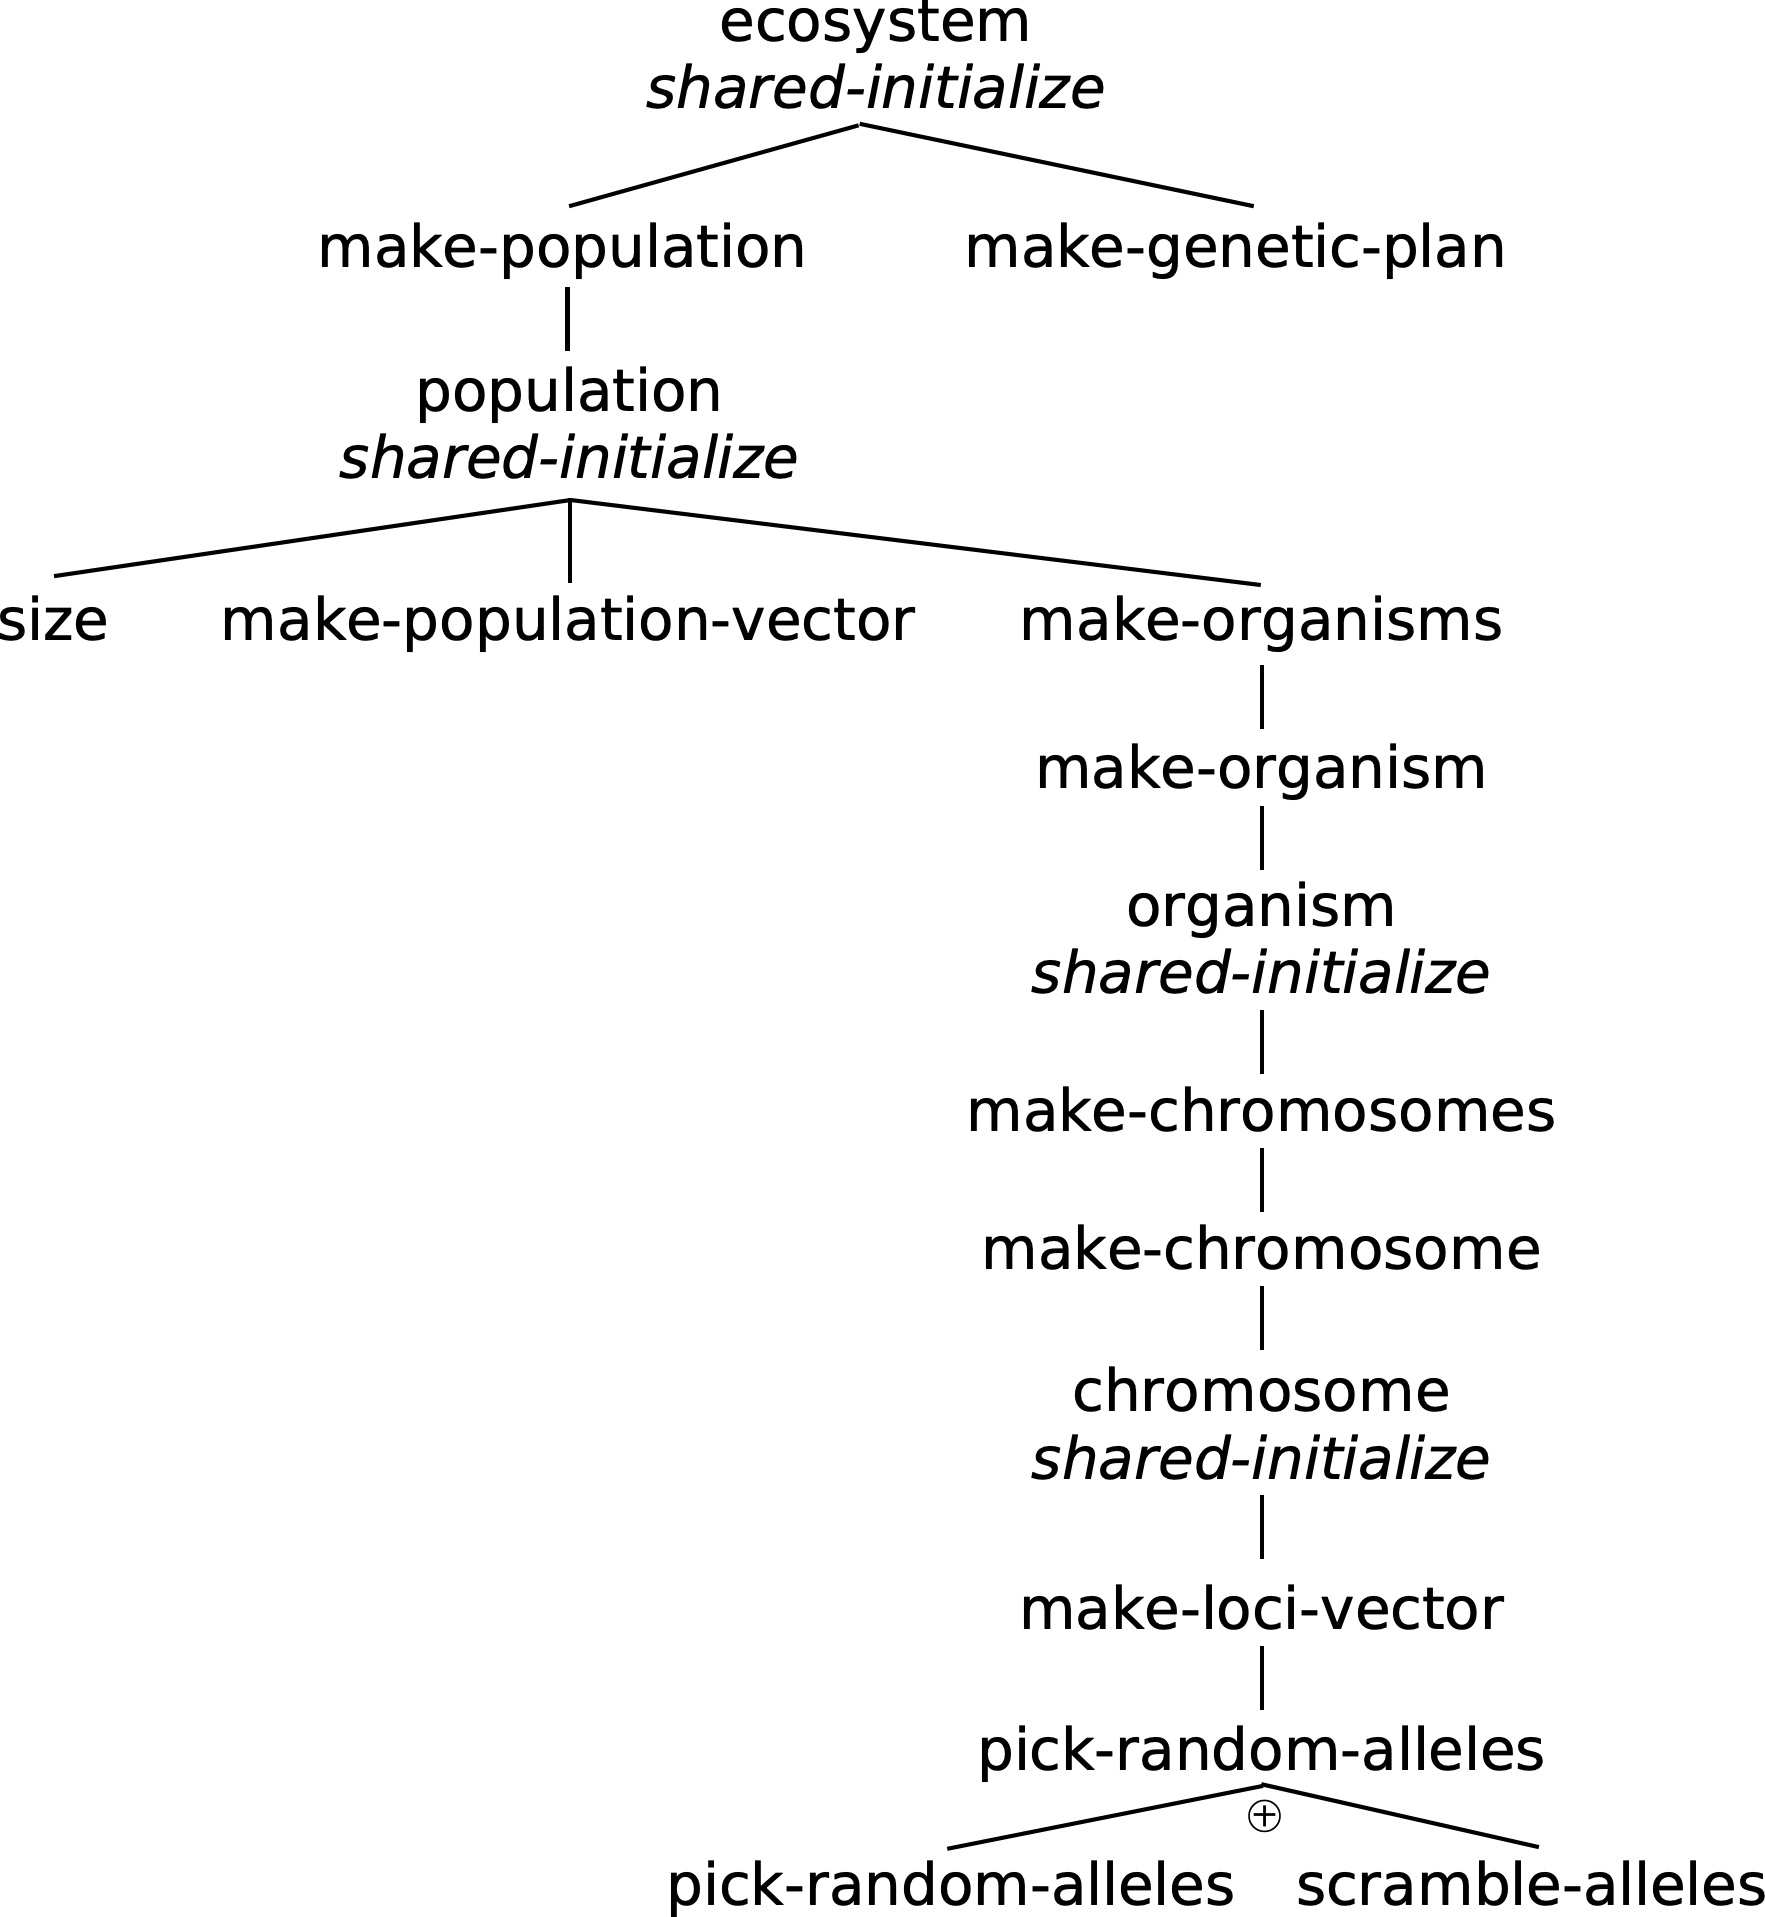
\includegraphics[width=\textwidth]{initialization-tree.eps}
  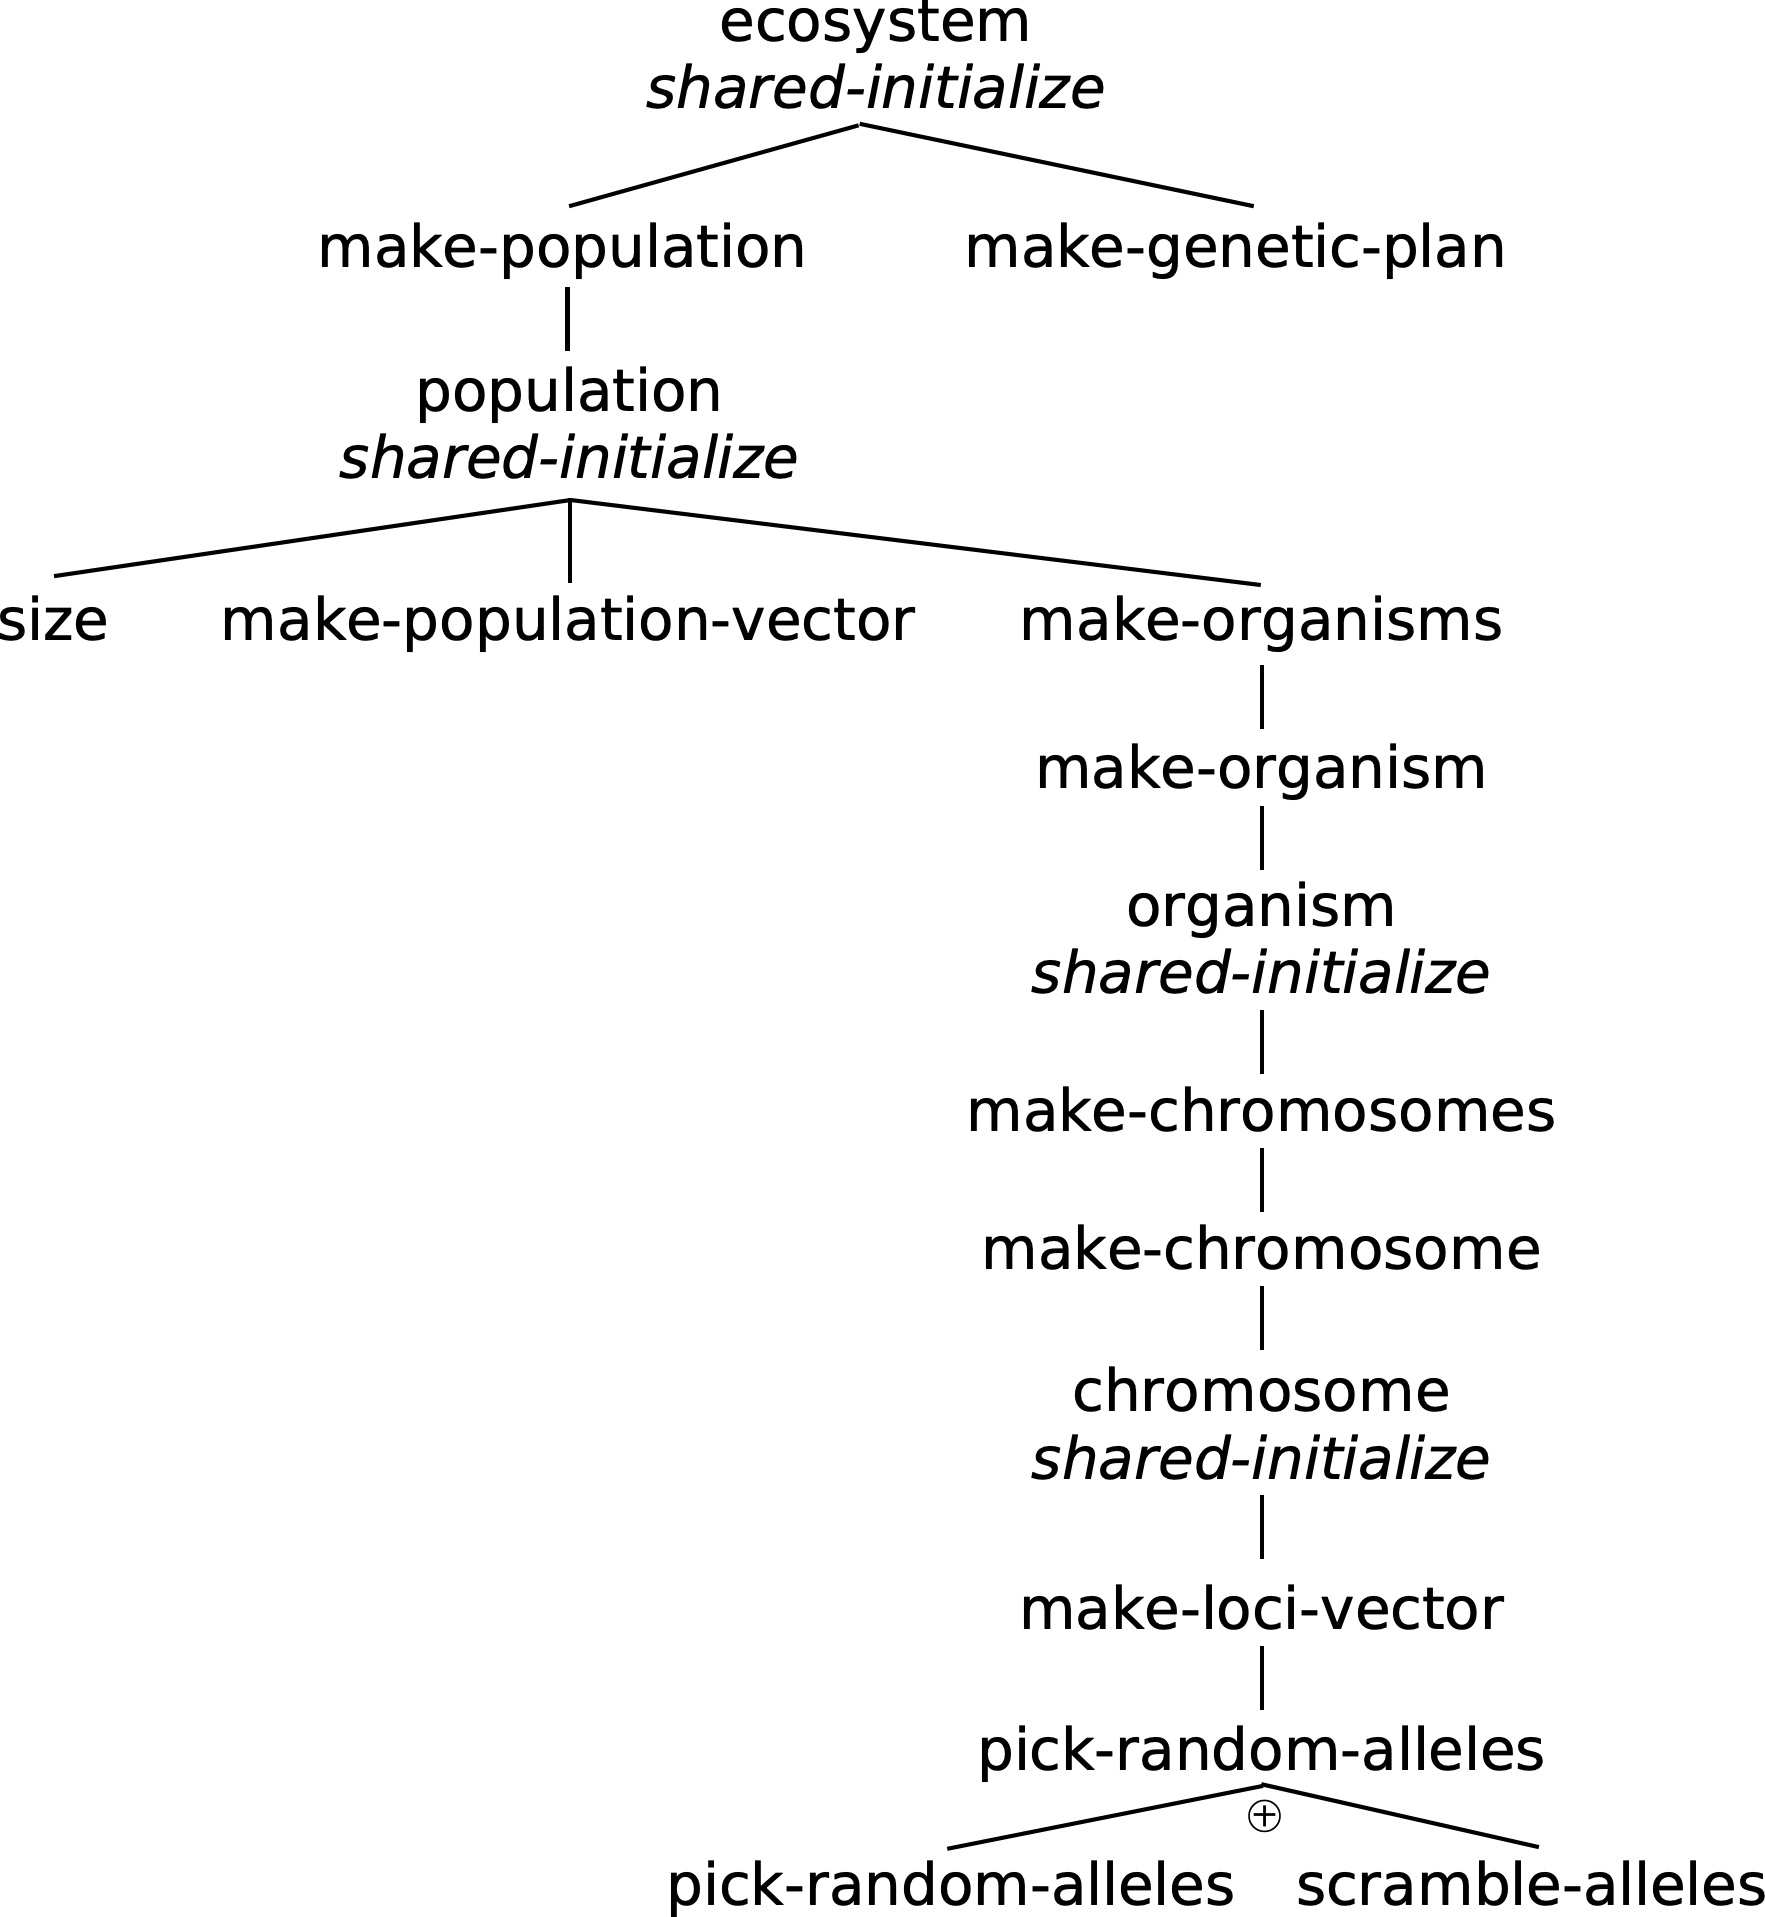
\includegraphics[width=0.6\textwidth]{initialization-tree.png}
  \caption{Call hierarchy for initialization of \Geco's principle structures}
  \label{fig:initialization-tree}
\end{figure}

\begin{figure}
  \centering
  % 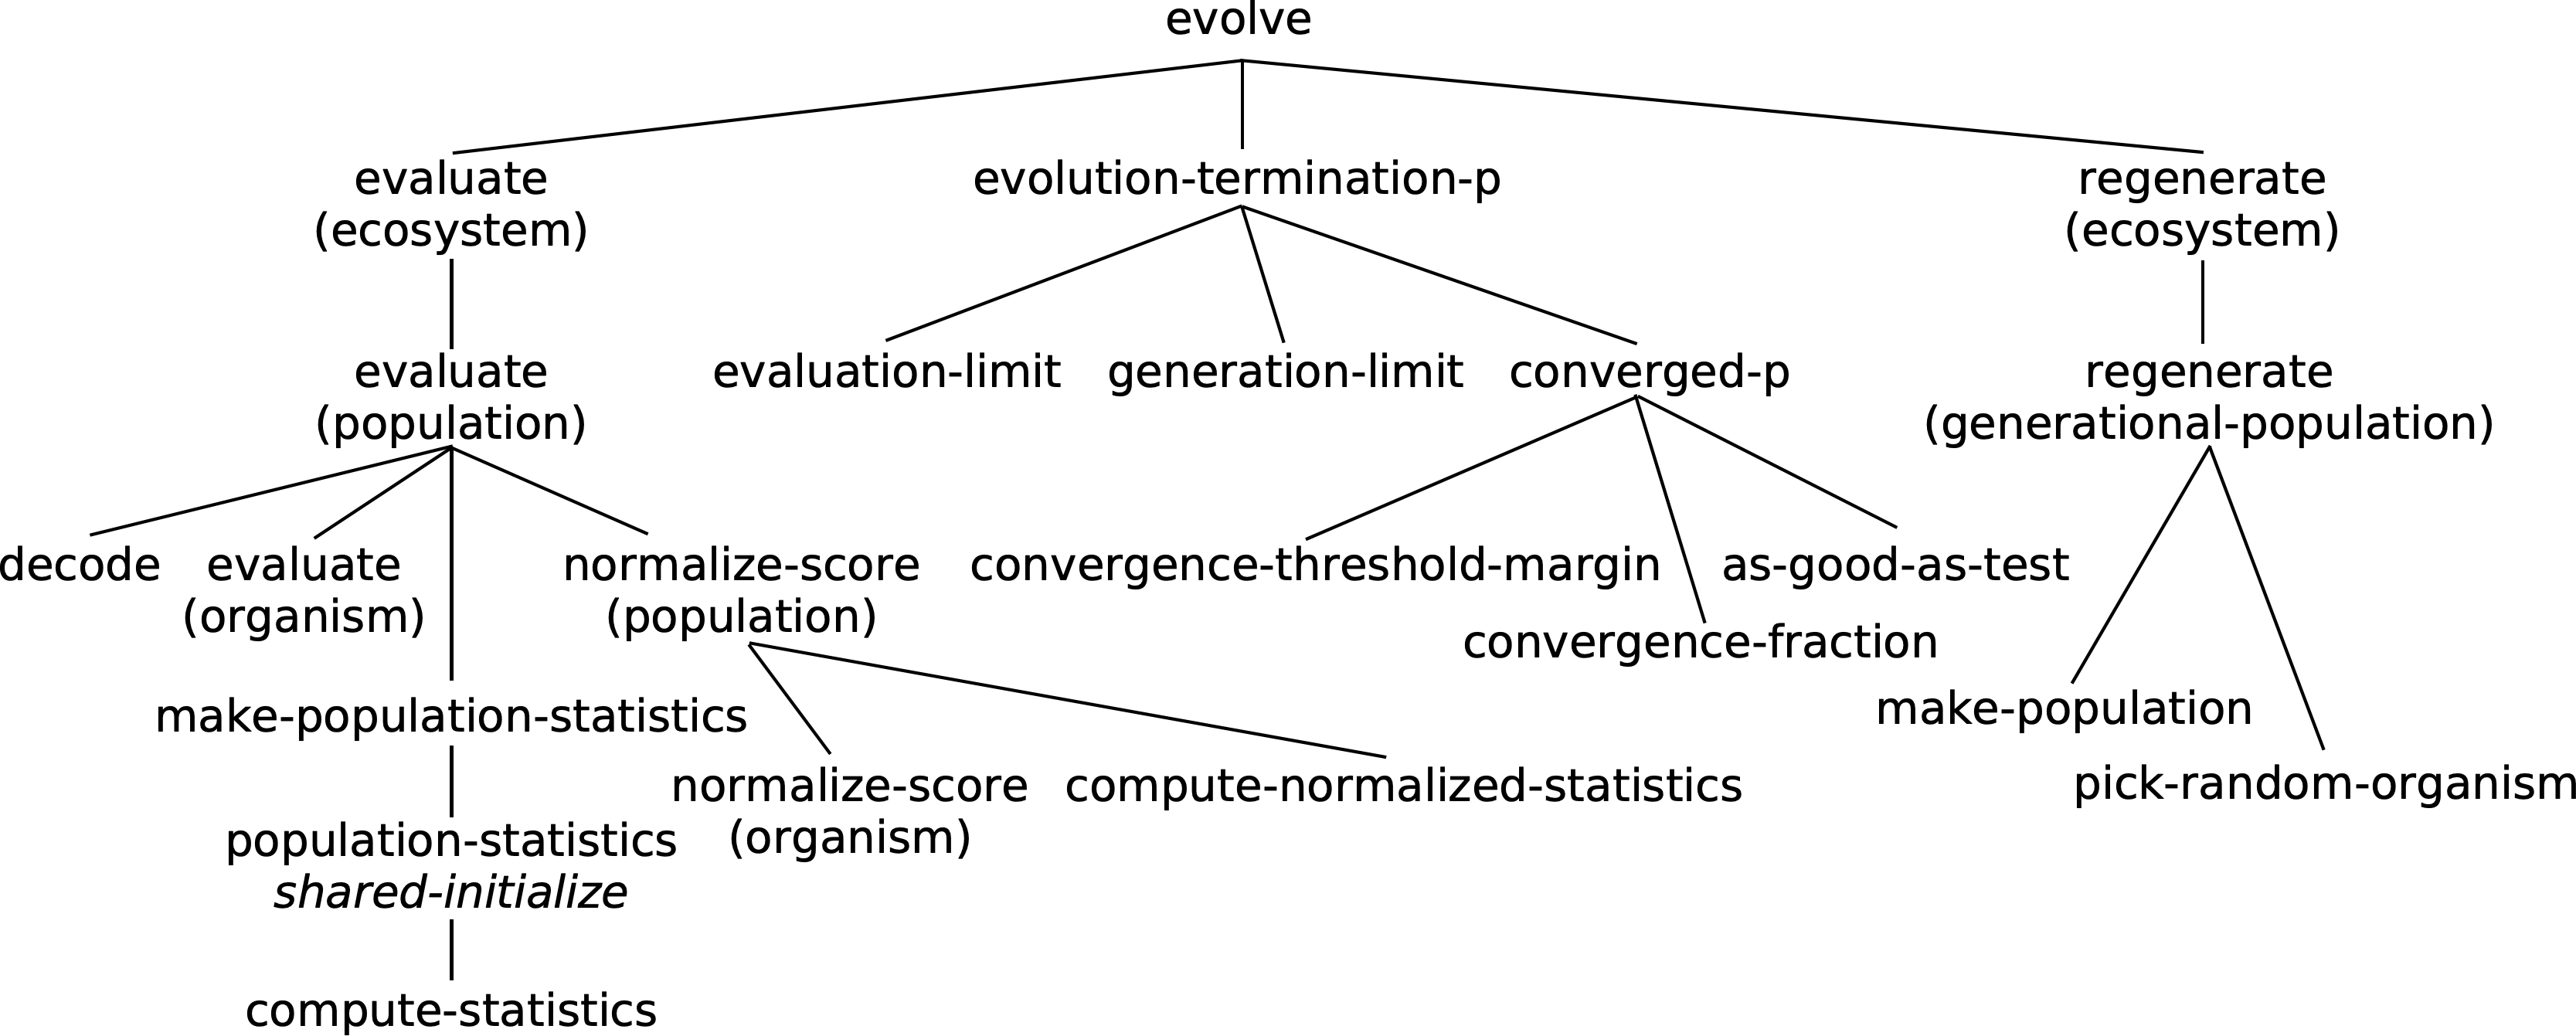
\includegraphics[width=\textwidth]{vert-evolve-tree.eps}
  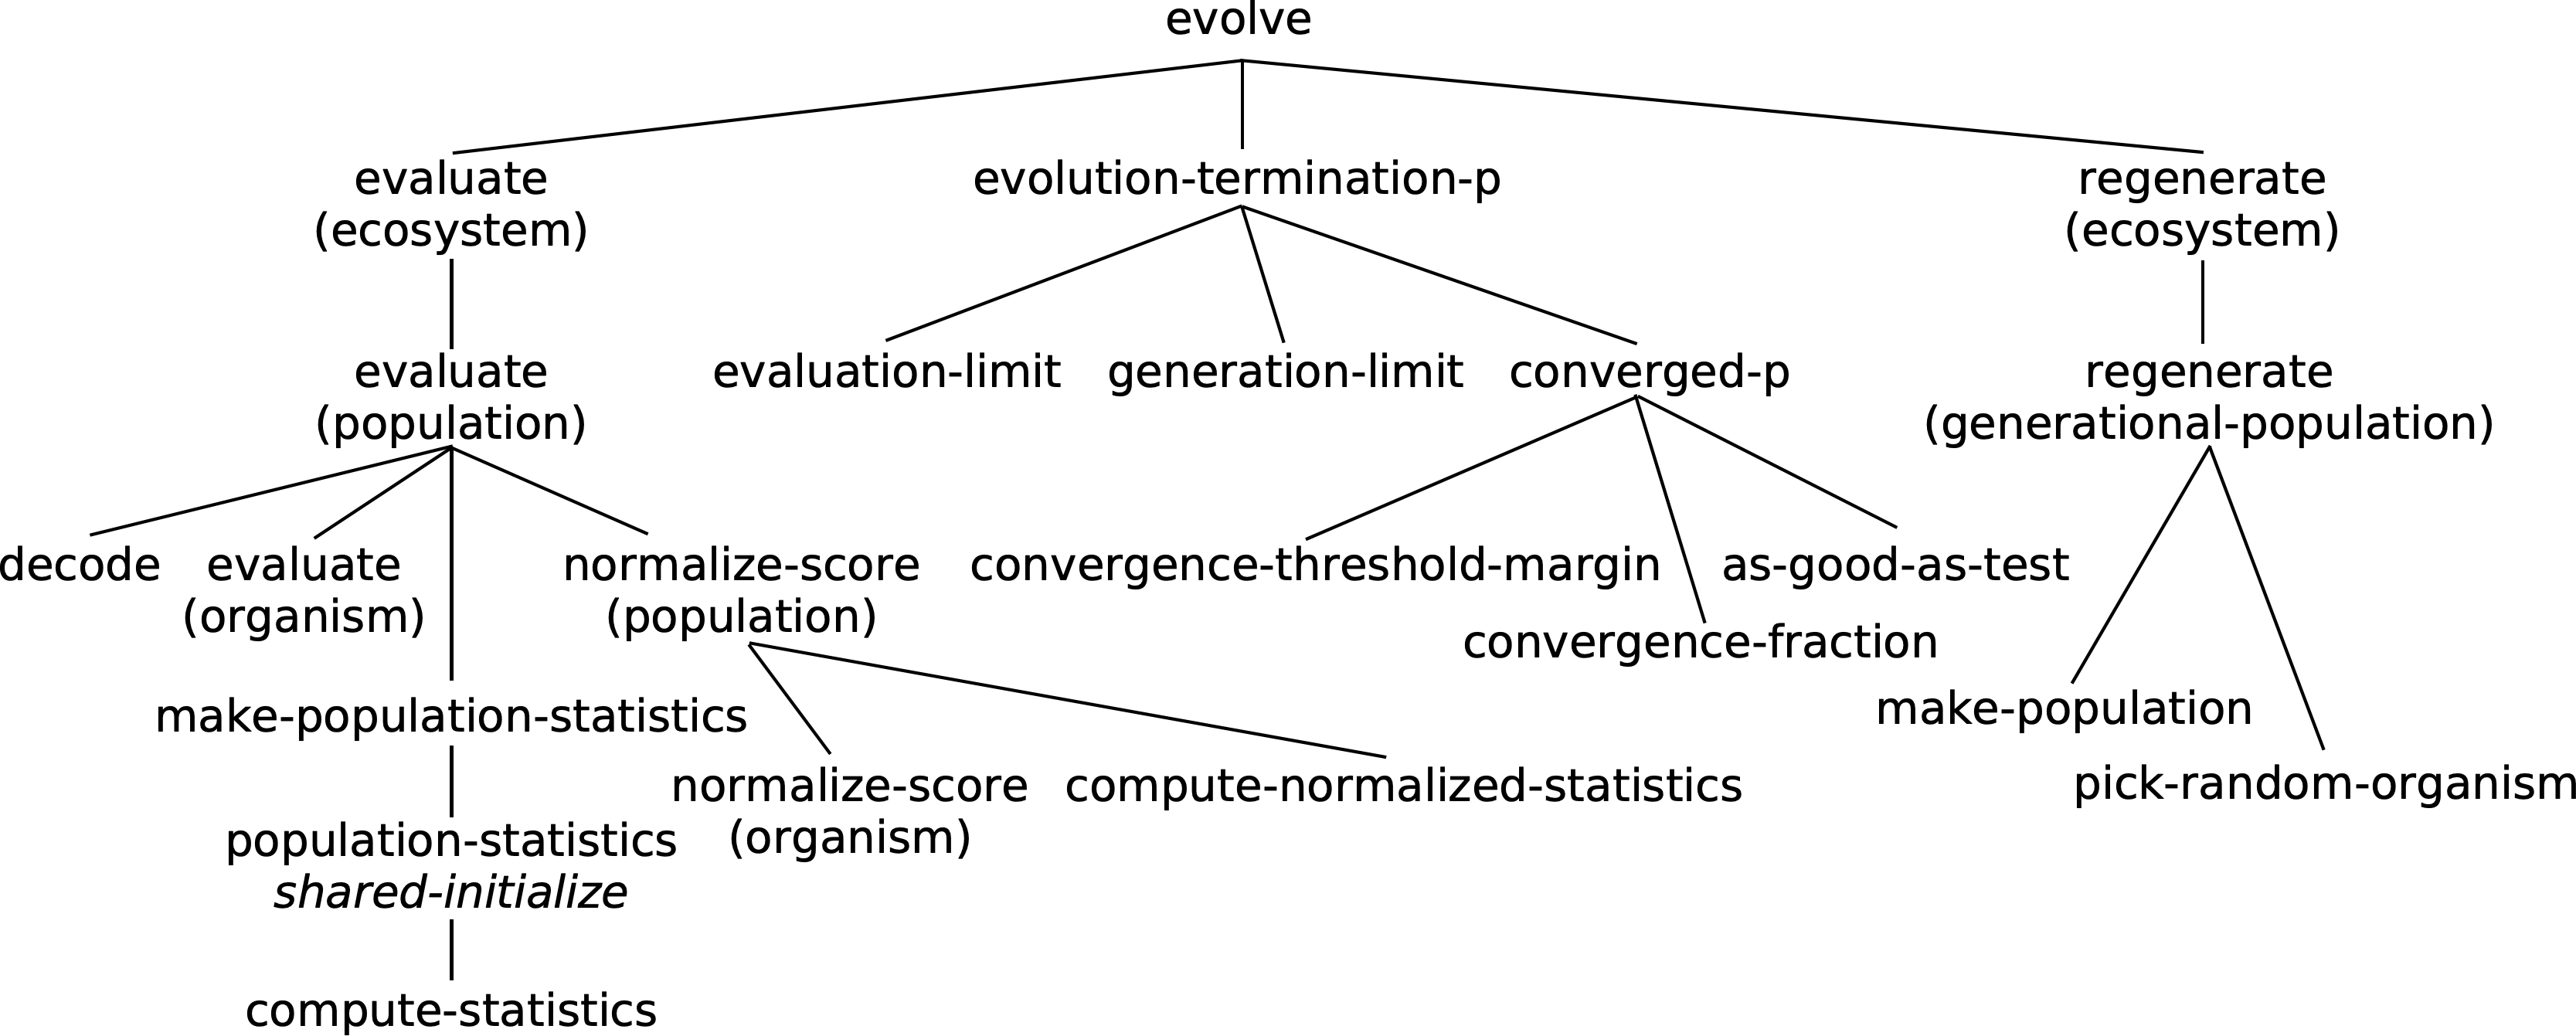
\includegraphics[width=\textwidth]{vert-evolve-tree.png}
  \caption{Call hierarchy for \Geco's evolutionary processing}
  \label{fig:evolve-tree}
\end{figure}

When supplied with the appropriate information, \geco\ can perform much of the
book-keeping, initialization, and control automatically.  This is made
possible by the built-in links between objects which are built upon the
\geco\ classes (see Figure~\ref{fig:class-interrelationships}).

\begin{figure}
  \centering	%% class-interrelationships.png is exported from class-interrelationships.pxd.pdf.cvd
  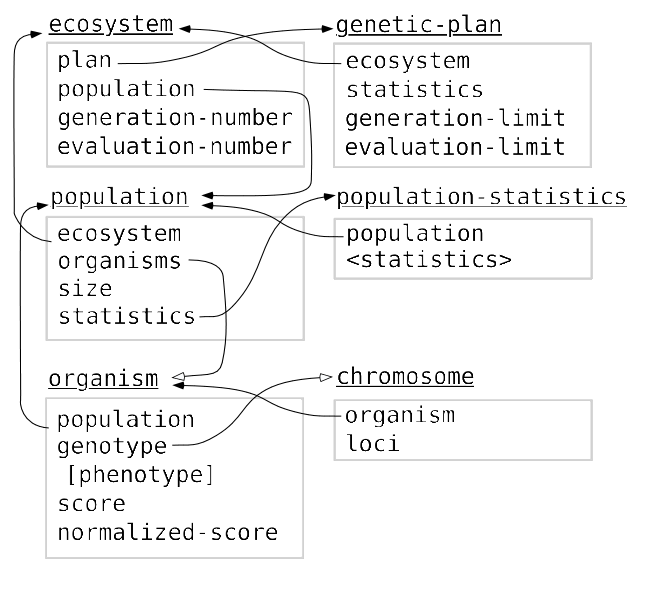
\includegraphics[width=0.75\textwidth]{class-interrelationships.png}
  % 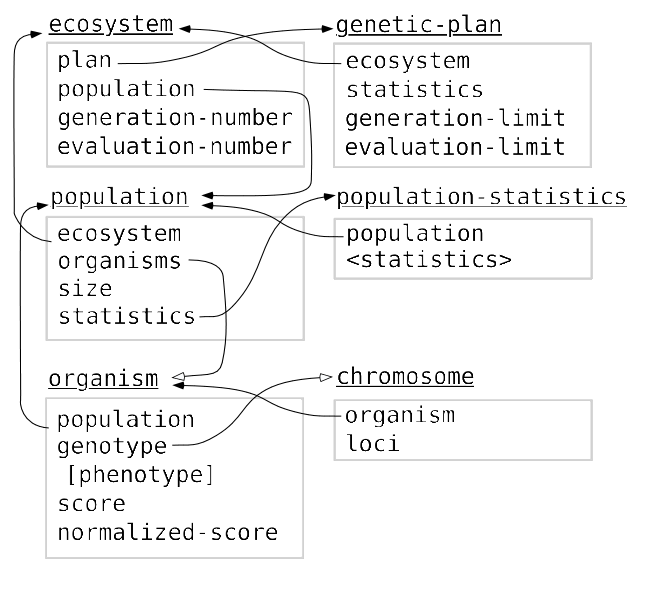
\includegraphics[]{class-interrelationships.png}
     \begin{center}
Solid head arrows indicate a one-to-one link;\\
hollow head arrows indicate a one-to-many link.
     \end{center}
  \caption{Interrelationships between \Geco\ objects}
  \label{fig:class-interrelationships}
\end{figure}



	% Copyright (C) 2020  George P. W. Williams, Jr.
\chapter{Details of GECO Classes and Functionality}

This chapter provides a more detailed discussion of each of \geco's 
classes, and the functionality implemented by their methods.   This functionality 
includes both the state retained by instances of each class (their {\em slots}),
and the functions (both generic and otherwise) which operate on those instances.

Even with all the functionality which \geco\ implements, it will still be
necessary to define some things which are specific to your application.
Generally this will be done by specializing \geco's classes (\ie, defining
some subclasses of \geco's builtin classes), and adding a few method
definitions to override and/or extend some of \geco's default behaviors.

Terminology Notes:

\begin{itemize}

\item In the material which follows, a statement which refers to `an instance of
\bold{a} {\it class-name} class' means that the instance is of the class
{\it class-name} or one of its subclasses. If the intent is to restrict the
instance to being of the named class, excluding subclasses, the wording will be
of the form `an instance of \bold{the} {\it class-name} class.'

\item In the descriptions of the methods, it will often be necessary to
distinguish between a generic function, a method for the generic function, and
the specific method supplied by \geco. A generic function and a method (as
specialized in the \term{flag line} above the description) are both parts of a
functional protocol which \geco\ expects to be honored.  A description
of a \geco-supplied method specifies that it
implements (fulfills) the requirements of this protocol.  \Geco\ may
define multiple methods (specialized for different classes) to implement
the generic function protocol for different classes.

\end{itemize}

For each class, the following sections will present the slots which 
are present in instances of the class (\ie, the values stored with each 
instance) and the functionality which has been defined for use with 
instances of the class (and its subclasses).
Generally, GAs implemented with \geco\ will not instantiate these classes.  
Instead, it will be more common to define subclasses which extend these 
classes (via added slots and methods) and specialize them (by overriding 
and/or extending inherited methods).


\section{The Ecosystem Class}

An \inxclass{ecosystem} is the highest level abstraction in a \geco\ implementation.
It is also the handle for manipulating a particular run of a GA. Since there may be
more than one instance of an \inxclass{ecosystem} in existence at one time, it is
possible to use \geco\ to create applications which use more than one GA at the same
time. The individual GAs could be competing, working on separate aspects of the same
problem, or they could be completely independent.
\filbreak
{\samepage

\Defclass {ecosystem}

\gap
\bold{Instance Allocated Slots}

  \Defslot {population}
  \defaccessor {population}

  An instance of a \inxclass{population} class.
  The population of an ecosystem is the set of organisms which are being 
  evolved.
\par}%end samepage

\filbreak

{\samepage
  \Defslotv {generation-number} {0}
  \defaccessor {generation-number}

  An integer, initially 0, which is 
  incremented each time the population enters a new {\em generation}.
  This happens each time the \inxgeneric{evolve}
  function is invoked on an \inxclass{ecosystem} instance (including
  \inxgeneric{evolve}'s recursive self-invocations). It should be noted
  that the actual creation of new members of the population (or creation
  of an entire new population) is expected to be handled by a \inxgeneric{regenerate}
  method specialized on a \inxclass{population} class, which
  is called by the default \geco-supplied \inxmethod{regenerate} method 
  specialized on \inxclass{ecosystem}.
\par}%end samepage

\filbreak

{\samepage
  \Defslotv {evaluation-number} {0}
  \defaccessor {evaluation-number}

  An integer, initially 0, which counts the number of times the 
  \inxgeneric{evaluate} function is applied to an \inxclass{organism} instance.
\par}%end samepage

\filbreak

{\samepage
  \Defslot {plan}
  \defaccessor {plan}

  An instance of a \inxclass{genetic-plan} class.
\par}%end samepage
\gap

\filbreak

The number of generations and evaluations are tracked by \geco\ so that the 
GA can be terminated based on the number of generations or evaluations 
exceeding some specific maximum limits, specified by the GA implementor.  
These limits are among the slots of the class \inxclass{genetic-plan}.

\filbreak
The \inxslot{population} and \inxslot{plan} are distinguished from the 
\inxclass{ecosystem} so that their classes may be specialized independently.  
Thus an instance of a single \inxclass{population} class may be manipulated 
using different \inxclass{plan}s, while instances of a single \inxclass{plan} may be 
used with different \inxclass{population}s.

\gap

\filbreak

{\samepage
	\bold{Instance Creation and Initialization}

The \inxclass{ecosystem} instance initialization has been extended by \geco\ by providing
a \cl{shared-initialize :AFTER} method for \inxclass{ecosystem}
to process the keyword arguments described below as follows:
\begin{itemize}
	\item If the call to \inxfun{make-instance}
	to create an instance of \inxclass{ecosystem} does not supply an initial population,
	then the \cl{:AFTER} method will initialize the \inxslot{population} slot using
	\inxgeneric{make-population}, with the values supplied via the \arg{:pop-class} and
	\arg{:pop-size} initargs.
	The call to \inxgeneric{make-population} also passes a value of \cl{t} for the \cl{:random}
	keyword argument, causing the initial population to be initialized to random organisms.
	(See Section~\ref{sec:population},
	page~\pageref{sec:population}.)
	
	\item Similarly, if a \inxclass{genetic-plan} instance is not supplied, then the \cl{:AFTER}
	method will initialize the \inxslot{plan} slot using \inxgeneric{make-genetic-plan}, with
	the value supplied via the \arg{:plan-class} initarg, and initializes the plan
	instance's \inxslot{generation-limit} and \inxslot{evaluation-limit} slots using the
	\arg{:gneration-limit} and \arg{:evaluation-limit} initargs. (See Section~\ref{sec:genetic-plan},
	page~\pageref{sec:genetic-plan}.)
\end{itemize}
The \inxgeneric{make-population} and \inxgeneric{make-genetic-plan} generic functions and
methods will be described subsequently, along with other \inxclass{ecosystem}-specialized
methods.
No special functions for the creation of \inxclass{ecosystem} instances have been defined,
since \inxgeneric{make-instance} and the standard \term{CLOS} protocol it follows provide all
the necessary functionality.

\par}%end samepage

\filbreak

{\samepage
\Definitarg {:plan-class}

  Provide the class for the \inxclass{genetic-plan} to be used by the
\inxclass{ecosystem}.
\par}%end samepage

\filbreak

{\samepage
\Definitarg {:pop-class}

  Provide the class for the \inxclass{population} instances to be created by
the \inxclass{ecosystem}.
\par}%end samepage

\filbreak

{\samepage
\Definitarg {:pop-size}

  Specifies the size to be used when the \inxclass{ecosystem} creates
\inxclass{population} instances.
\par}%end samepage

\filbreak

{\samepage
\Definitarg {:generation-limit}

This initarg is intended to specify the maximum number of generations which the ecosystem
will be allowed to evolve.
This limit is typically enforced by the \inxgeneric{evolution-termination-p} function
(see page~\pageref{evolution-termination-p}).
	
\par}%end samepage

\filbreak

{\samepage
\Definitarg {:evaluation-limit}

This initarg is intended to specify the maximum number of evaluations which the ecosystem
will be allowed to perform.
This limit is typically enforced by the \inxgeneric{evolution-termination-p} function
(see page~\pageref{evolution-termination-p}).

\par}%end samepage

\filbreak
\gap

{\samepage
\bold{Specialized Methods}

No special functions for the creation of \inxclass{ecosystem} instances have been defined
in \geco, since the \inxgeneric{make-instance} function and the standard \term{CLOS} protocol
it follows provide all the necessary functionality.
\par}% end \samepage

\filbreak

{\samepage

% use \Eggeneric so the CLOS generic isn't indexed
\Eggeneric shared-initialize {standard-object slot-names \rest initargs}
\defaftermethod shared-initialize {(ecosystem \inxclass{ecosystem}) slot-names \rest initargs
	\key :plan-class :pop-class :pop-size :generation-limit :evaluation-limit}

This method extends the initialization for \inxclass{ecosystem} instances to provide for the 
automatic creation and initialization of the \inxclass{population} and \inxclass{genetic-plan}
instances and slots.
The \inxgeneric{make-population} and \inxgeneric{make-genetic-plan} generic functions (described
next) are provided to support customization of these actions.
The call to \inxgeneric{make-population} in the default \geco-supplied method
passes a value of \cl{t} for the \cl{:random} keyword
argument, causing the initial population to be initialized to random organisms.
If \cl{:generation-limit} and \cl{evaluation-limit} are specified, the \inxslot{generation-limit}
and \inxslot{evaluation-limit} slots in the \inxclass{genetic-plan} instance are also initialized.
\par}% end \samepage

\filbreak

{\samepage

\Defgeneric make-population {ecosystem population-class \key :size :random}
\defmethod make-population {(ecosystem \inxclass{ecosystem}) population-class
	\key :size :random}
	\label{method:make-population}

This function provides an abstract interface to creation of a \inxclass{population} instance
to store in the \inxslot{population} slot of \arg{ecosystem}.
The primary \geco-supplied method
invokes \inxgeneric{make-instance} on the class \arg{population-class}, passing
the \arg{:size} argument, which determines the population size, and the
\arg{:random} argument, which if it is non-\cl{nil}, will cause the population to
be created with random organisms (intended for creation of the initial population).
It also returns the \inxclass{population} instance thus created.
\par}%end samepage

\filbreak

{\samepage
\Defgeneric make-genetic-plan {ecosystem genetic-plan-class}
\defmethod make-genetic-plan {(ecosystem \inxclass{ecosystem}) genetic-plan-class}
	\label{method:make-genetic-plan}

This function provides an abstract interface to creation of the \inxclass{genetic-plan}
instance for \arg{ecosystem}.  The \geco-supplied primary method invokes
\inxgeneric{make-instance} on \arg{genetic-plan-class}, and also supplies
\arg{ecosystem} so that the plan can be linked to the ecosystem (and vice-versa).
It also returns the \inxclass{genetic-plan} instance thus created.
\par}%end samepage

\filbreak

{\samepage
\Defgeneric evolve {ecosystem}
\defmethod evolve {(ecosystem \inxclass{ecosystem})}

This is the principle function which will be used by GA developers to invoke
their algorithm. The \geco-supplied primary method calls \inxmethod{evaluate} on
\arg{ecosystem}, and if the termination\index{termination} condition has not been
reached (see \inxgeneric{evolution-termination-p}), creates a new generation of
its \inxslot{population} via the \inxgeneric{regenerate} function, and
recurses to evolve some more\footnote{See the discussion in the footnote on
page~\pageref{recursive-vs-iterative-evolve}}.
The value returned by this function is not defined.
\par}%end samepage

\filbreak

{\samepage  
\Defgeneric evaluate {thing genetic-plan}
\defmethod evaluate {(ecosystem \cl{ecosystem}) genetic-plan}

The purpose of this function is to cause \arg{thing} to be evaluated according to
the specified \term{genetic plan}. The \geco-supplied primary method for
\inxclass{ecosystem} instances evaluates \arg{ecosystem} by calling
\inxgeneric{evaluate} on its \inxslot{population} with \arg{genetic-plan}. (Also
see the \inxmethod{evaluate} method specialized for the class \inxclass{population}, on
page~\pageref{evaluate-population}.)
The value returned by this function is not defined.
\par}%end samepage

\filbreak


\section{The Population Class} \label{sec:population}

A population is the most global structure upon which a GA operates. Although
\term{genetic operator}s are applied to the members (\term{organism}s in 
\geco's terminology, though they are often called
\ital{individuals}) of a population, it is at the level of the population that
the GA is really working.

\filbreak

{\samepage
\Defclass {population}

Instances of \inxclass{population} classes collect all the \inxclass{organism} 
instances of a generation.
\par}%end samepage

\gap

\filbreak

{\samepage
\bold{Instance Allocated Slots}

\Defslot {ecosystem}
\definitarg {:ecosystem}
\defaccessor {ecosystem}

Provides a link back to the \inxclass{ecosystem} instance to which the population belongs.
\par}%end samepage

\filbreak

{\samepage
\Defslot {organisms}
\defaccessor {organisms}

A vector, which contains all the \inxclass{organism} instances in the population.
\par}%end samepage

\filbreak

{\samepage
\Defslotv {size} {nil}
\definitarg {:size}
\defaccessor {size}

Either \cl{nil} or an integer, which indicates the size of the population, \ie,
the size of the vector in the \inxslot{organisms} slot. When \cl{nil}, the
organism vector will not be created automatically. \par}%end samepage

\filbreak

{\samepage
\Defslot {statistics}
\definitarg {:statistics}
\defaccessor {statistics}

An instance of a \inxclass{population-statistics} class, which holds statistics
\geco\ needs for the population. The \inxclass{population-statistics} class is
distinct from the \inxclass{population}class so that their sub-classes and methods may 
be specialized independently. 
\par}%end samepage

\gap
\filbreak

{\samepage

\bold{Instance Creation and Initialization}

The generic function \inxgeneric{make-population} (see page~\pageref{method:make-population})
is the \geco\ interface for creation of \inxclass{population} instances.

The initialization for instances of \inxclass{population} has been extended to
provide for automatic creation and initialization of the \inxslot{organisms}
vector. The functions \inxgeneric{make-organisms-vector} and
\inxgeneric{make-organisms} are used to permit customization of these
initialization actions; \inxgeneric{make-organisms-vector} is called when the
\inxslot{size} slot has a non-\cl{nil} value, and \inxgeneric{make-organisms} is
called only when both \inxslot{size} and \inxinitarg{:random} (below) have
non-\cl{nil} values. It is the responsibility of the \term{genetic plan} to
create the organisms after the initial generation.
\par}%end samepage

\filbreak

{\samepage
The \inxclass{population} instance initialization has been extended to support the following
additional initarg:

\Definitarg {:random}

The value of this keyword is passed to \inxgeneric{make-organisms}, and is intended
to support automatic initialization of the initial population to random organisms.
\par}%end samepage
\gap
  
\filbreak

{\samepage

\bold{Specialized Methods}

Note that most (if not all) of the generic functions in
Section~\ref{sec:selection-methods}, Selection Methods, have methods which
are specialized on the \inxclass{population} class.

\filbreak

{\samepage
	
% use \Eggeneric so the CLOS generic isn't indexed
\Eggeneric shared-initialize {standard-object slot-names \rest initargs}
\defaftermethod shared-initialize {(pop \inxclass{population}) slot-names \rest initargs
	\key :random}

This method extends the initialization for \inxclass{population} instances to provide for the 
automatic creation and initialization of the \inxclass{organism} instances for the population.
In the \geco-supplied default method, if the \inxslot{organisms} slot of 
\arg{pop} is unbound, the \inxgeneric{make-organisms-vector} generic function
(see below) is invoked to initialize the \inxslot{organisms}
slot; and then, if the \arg{:random} keyword argument is non-\cl{nil}, the
\inxgeneric{make-organisms} function (see below) is invoked to initialize
the population's organism vector to random organisms.
\par}% end \samepage

\filbreak

{\samepage
\Defgeneric make-organisms-vector {population size}
\defmethod make-organisms-vector {(population \inxclass{population}) size}

This function provides an abstract interface to creation of the population's
organisms vector (the vector which holds \arg{population}'s organisms). The
\arg{size} argument determines the size of the vector. The \geco-supplied primary
method uses the Common Lisp function \cl{make-array} to create an array of the
specified size.
It also returns the the array thus created.
\par}%end samepage

\filbreak

{\samepage
\Defgeneric make-organisms {population \key :random}
\defmethod make-organisms {(population \inxclass{population}) \key :random}

This function provides an abstract interface to creation of the organisms in
\arg{population}'s organisms vector. The \arg{:random} argument, when
non-\cl{nil}, causes all the new organisms to be random (\ie, have randomly
chosen chromosomes). The \geco-supplied primary method invokes
\inxgeneric{make-organism} for each position in the organisms vector. The
\arg{:random} argument is passed to each call to \inxgeneric{make-organism}.
The value returned by this function is not defined.
\par}%end samepage

\filbreak

{\samepage
\Defgeneric make-organism {population \key :random :no-chromosome}
\defmethod make-organism {(population \inxclass{population}) \key :random :no-chromosome}
	\label{method:make-organism}

This function provides an abstract interface to creation of a single organism
based on the \inxgeneric{organism-class} of \arg{population}. The \arg{:random}
argument, when non-\cl{nil}, causes the new organism to be random (\ie, have
randomly chosen chromosomes). The \arg{:no-chromosome} argument, when
non-\cl{nil}, causes the organism to be created without chromosomes, avoiding
wasted work when the chromosomes will be supplied by other mechanisms, \eg,
\term{genetic operator}s. The \geco-supplied primary method passes \arg{population} to
the call to \inxgeneric{make-instance} so that the organism can have a back-link
to the population to which it belongs. The \arg{:random} and
\arg{:no-chromosomes} arguments are passed to \inxgeneric{make-instance}.
It also returns the the \inxclass{organism} instance thus created.
\par}%end samepage

\filbreak

{\samepage
\Defgeneric organism-class {population}

This function returns the class to be used to create organisms which will become members
of \arg{population}. The GA developer {\em must implement the primary method} for all
subclasses of the class \inxclass{population}. \Geco\ does not provide a default primary method
specialized on the \inxclass{population} class.\footnote{There are comments at the beginning
of the {\tt generics.lisp} file which summarize the functions which should or must be
defined to implement a working GA using \geco.}
\par}%end samepage

\filbreak

{\samepage
\Defgeneric evaluate {thing genetic-plan}
\defmethod evaluate {(population \inxclass{population}) (genetic-plan \inxclass{genetic-plan})}
\label{evaluate-population}

This function evaluates \arg{thing} according to \arg{genetic-plan}. This method
assures that each organism in \arg{population} is evaluated. The \geco-supplied
primary method only calls \inxgeneric{evaluate} on an organism if the organism
doesn't already have a \term{score} in its \inxslot{score} slot. After
\arg{population} has been evaluated, \inxgeneric{normalize-score} and
\inxgeneric{make-population-statistics} are called to assure that normalized
scores and statistics have been computed for the population.
The value returned by this function is not defined.
\par}%end samepage

\filbreak

{\samepage
\Defgeneric make-population-statistics {population}
\defmethod make-population-statistics {(population \inxclass{population})}
	\label{method:make-population-statistics}

This function provides an abstract interface to creation of the
\inxclass{population-statistics} instance for \arg{population}, based on the
\inxgeneric{population-statistics-class} of \arg{population}. The \geco-supplied
primary method passes \arg{population} to \inxgeneric{make-instance} so that the instance can
have a back-link to the population to which it belongs.
It also returns the \inxclass{population-statistics} instance thus created.
\par}%end samepage

\filbreak

{\samepage
\Defgeneric compute-statistics {population}
\defmethod compute-statistics {(population \inxclass{population})}

This function provides an abstract interface for computing statistics for
\arg{population}. This method provieds a place for a population class to provide
for customization of statistics computation. The \geco-supplied primary method
simply calls \inxgeneric{compute-statistics} on the statistics instance of
\arg{population}. (Also see the description of \inxmethod{compute-statistics}
on page~\pageref{compute-population-statistics},
specialized on the class \inxclass{population-statistics}, and
Section~\ref{sec:pop-stats-class}, which details the statistics that are computed.)
The value returned by this function is not defined.
\par}%end samepage

\filbreak

{\samepage
\Defgeneric compute-binary-allele-statistics {population}
\defmethod compute-binary-allele-statistics {(population \inxclass{population})}

This function returns a list of vectors (one per binary chromosome in the
organisms of \arg{population}) of counts (\cl{fixnum}s), by locus, of non-zero
alleles. For example, if the organisms in a population contain $c$ binary
chromosome (and any number of non-binary chromosomes), and each binary chromosome
contains $b$ loci, then this function will return a list containing $c$ vectors
of $b$ fixnums. Each \cl{fixnum} in the returned vectors is a count of non-zero
alleles in the entire population at the locus whose index corresponds to the
index into the $c^{\rm th}$ vector of counts. \Eg, if the third count in the
first vector is 7, then the entire population contains 7 non-zero alleles in
locus 3 of the first binary chromosome of each organism.
\par}%end samepage

\filbreak

{\samepage
\Defgeneric normalize-score {thing plan}
\defmethod normalize-score {(population \inxclass{population})
                            \hbox{(genetic-plan \inxclass{genetic-plan})}}

This function computes the normalized
\term{score}(s)\index{score!normalization}\index{normalization} for \arg{thing}.
This method computes the normalized scores for all organisms in \arg{population}.
The \geco-supplied primary method for \inxclass{population} invokes
\inxgeneric{normalize-score} (see page \pageref{method:normalize-score:organism})
for each organism in \arg{population}, according to the \arg{genetic-plan}, and
updates \cl{(statistics \arg{population})} with normalized values using the function
\inxgeneric{compute-normalized-statistics}.
The value returned by this function is not defined.

[Note that \geco\ version 2.1 changed the calling sequence for this generic function and all its methods.]
\par}%end samepage

\filbreak

There are a number of different ways to normalize\index{normalization} the
scores. With some plans and evaluation functions, it may not even be necessary,
though beware that the score should always be $\ge 0$ (see Chapter 4 of
\cite{ga:goldberg}, under the sections on Scaling Mechanisms and Ranking
Procedures).

\filbreak

{\samepage
\Defgeneric population-statistics-class {population}
\defmethod population-statistics-class {(population \inxclass{population})}

This function returns the population-statistics class which will be used for
\arg{population.} The \geco-supplied primary method specialized for the
\inxclass{population} class returns \inxclass{population-statistics}.
\par}%end samepage

% This function could be performed by \cl{:allocation :per-class} slots 
% if and when they can be implemented portably in Common Lisp.

\filbreak

{\samepage
\Defgeneric converged-p {population}
\defmethod converged-p {(population \inxclass{population})}
	\label{population:converged-p}
This function is a predicate which indicates whether \arg{population} has
\concept{converged}, which is useful as a termination\index{termination}
condition. The \geco-supplied primary method defines convergence as
either of the following:
\par}%end samepage

\filbreak

{\samepage
  \begin{enumerate}
    \item All organisms in \arg{population} have the same \inxslot{score}; or
    \item At least a portion of \arg{population} (specified by the
        \inxgeneric{convergence-fraction} function) has a 
        \inxslot{normalized-score} which is {\em as good as} the value specified by the
        \inxgeneric{convergence-threshold-margin} function.
  \end{enumerate}
}%end samepage

\filbreak

Note that this allows \geco\ to either {\em maximize} or {\em minimize}
\term{scores}. The mechanism for determining whether \geco\ maximizes or minimizes,
and hence how it determines {\em as good as} or {\em better than}, is determined by
mixing one of two classes with the population class used by the GA. These
\term{mixin classes} are described below, in section
\ref{sec:population-mixin-classes}.

\filbreak

{\samepage
\subsection{Subclasses of Population}

\Defclassv {generational-population} {population}

This class is a subclass of \inxclass{population} which provides explicit support
for the `standard' generational style of GA. The class has no
slots, but methods described elsewhere specialize on this class (see
\inxmethod{regenerate}, page~\pageref{method:regenerate}).
\par}%end samepage
\filbreak

Eventually \geco\ may contain support for other styles of population handling,
possibly including parallel sub-populations, steady-state populations, \etc.

\gap
\filbreak

{\samepage
\bold{Instance Creation and Initialization}

The generic function \inxgeneric{make-population} (see
page~\pageref{method:make-population}) is the \geco\ interface for creation
of instances of \inxclass{population} and its subclasses.
\par}%end samepage

\filbreak

{\samepage
\subsection{Population Mixin Classes}	\label{sec:population-mixin-classes}

\Defclass {maximizing-score-mixin}
\defclass {minimizing-score-mixin}

Neither of these classes has any slots or has special provisions for
instance creation or initialization.
\par}%end samepage

\gap

\filbreak

{\samepage

\bold{Specialized Methods}

Both classes implement methods for the following generic functions:

\Defgeneric maximizing-p {population}
\defmethod maximizing-p {(population \inxclass{maximizing-score-mixin})}
\defmethod maximizing-p {(population \inxclass{minimizing-score-mixin})}
\Defgeneric minimizing-p {population}
\defmethod minimizing-p {(population \inxclass{maximizing-score-mixin})}
\defmethod minimizing-p {(population \inxclass{minimizing-score-mixin})}

These functions permit algorithms to efficiently determine whether the
\arg{population} is minimizing or maximizing.  The \geco-supplied methods
return either \cl{t} or \cl{nil} as appropriate for their class.
\par}%end samepage

%These functions could all be performed by \cl{:allocation :per-class} slots if
%and when they can be implemented portably in Common Lisp.

\filbreak

{\samepage
\Defgeneric convergence-fraction {population}
\defmethod convergence-fraction {(population \inxclass{maximizing-score-mixin})}
\defmethod convergence-fraction {(population \inxclass{minimizing-score-mixin})}

This function returns the convergence-fraction value which should be used for
\arg{population} by the \inxgeneric{converged-p} function. The \geco-supplied
primary methods for both the \inxclass{maximizing-score-mixin} and the
\inxclass{minimizing-score-mixin} classes return $0.95$. These values are not
necessarily the {\em right} numbers in any real sense, but they are probably
reasonable for many applications. Some applications may want to provide different
values, and possibly even adaptive methods for specialized subclasses.
\par}%end samepage

\filbreak

{\samepage
\Defgeneric convergence-threshold-margin {population}
\defmethod convergence-threshold-margin {(population \inxclass{maximizing-score-mixin})}
\defmethod convergence-threshold-margin {(population \inxclass{minimizing-score-mixin})}

This function returns the convergence-threshold-margin value which should be used
for \arg{population} by the \inxgeneric{converged-p} function. The \geco-supplied
primary method provided for the \inxclass{maximizing-score-mixin} class returns
$0.95$, and the method provided for the \inxclass{minimizing-score-mixin} class
returns $0.05$. These values are not necessarily the {\em right} numbers in any real
sense, but they are probably reasonable for many applications. Some applications may
want to provide different values, and possibly even adaptive methods for specialized
subclasses. 
\par}%end samepage

\filbreak

{\samepage
\Defgeneric as-good-as-test {population}
\defmethod as-good-as-test {(population \inxclass{maximizing-score-mixin})}
\defmethod as-good-as-test {(population \inxclass{minimizing-score-mixin})}

This function returns a function of two numeric arguments, which when applied to
\inxslot{score}s from organisms in \arg{population}, indicates whether or not the first
score is as good as the second. The \geco-supplied primary method for the
\inxclass{maximizing-score-mixin} class returns \cl{#'>=}, and the method provided
for the \inxclass{minimizing-score-mixin} class returns \cl{#'<=}.
\par}%end samepage

\filbreak

{\samepage
\Defgeneric better-than-test {population}
\defmethod better-than-test {(population \inxclass{maximizing-score-mixin})}
\defmethod better-than-test {(population \inxclass{minimizing-score-mixin})}

This function returns a function of two numeric arguments, which when applied to
\inxslot{scores} from organisms in \arg{population}, indicates whether or not the first
score is better than the second. The \geco-supplied primary method provided
for the \inxclass{maximizing-score-mixin} class returns \cl{#'>}, and the method
provided for the \inxclass{minimizing-score-mixin} class returns \cl{#'<}.
\par}%end samepage

\filbreak

{\samepage
\Defgeneric best-organism {population}
\defmethod best-organism {(population \inxclass{maximizing-score-mixin})}
\defmethod best-organism {(population \inxclass{minimizing-score-mixin})}

This function returns the best organism in the corresponding population from
population statistics of \arg{population}. The \geco-supplied primary method for the
\inxclass{maximizing-score-mixin} class uses \inxgeneric{max-organism}, and the method
provided for the \inxclass{minimizing-score-mixin} class uses \inxgeneric{min-organism}.
\par}%end samepage

\filbreak

{\samepage
\Defgeneric worst-organism {population}
\defmethod worst-organism {(population \inxclass{maximizing-score-mixin})}
\defmethod worst-organism {(population \inxclass{minimizing-score-mixin})}

This function returns the best organism in the corresponding population from
population statistics of \arg{population}. The \geco-supplied primary method for the
\inxclass{maximizing-score-mixin} class uses \inxgeneric{min-organism}, and the method
provided for the \inxclass{minimizing-score-mixin} class uses \inxgeneric{max-organism}.
\par}%end samepage

\filbreak

{\samepage
\Defgeneric best-organism-accessor {population}
\defmethod best-organism-accessor {(population \inxclass{maximizing-score-mixin})}
\defmethod best-organism-accessor {(population \inxclass{minimizing-score-mixin})}

This function returns a function which can be applied to an instance of the
\inxclass{population-statistics} class of \arg{population} to obtain the best organism in the
corresponding population. The \geco-supplied primary method for the
\inxclass{maximizing-score-mixin} class returns \cl{#'}\inxgeneric{max-organism},
and the method provided for the \inxclass{minimizing-score-mixin} class returns
\cl{#'}\inxgeneric{min-organism}.
\par}%end samepage \filbreak

\filbreak

{\samepage
\Defgeneric worst-organism-accessor {population}
\defmethod worst-organism-accessor {(population \inxclass{maximizing-score-mixin})}
\defmethod worst-organism-accessor {(population \inxclass{minimizing-score-mixin})}

This function returns a function which can be applied to an instance of the
\inxclass{population-statistics} class of \arg{population} to obtain the worst organism in
the corresponding population. The \geco-supplied primary method for the
\inxclass{maximizing-score-mixin} class returns \cl{#'}\inxgeneric{min-organism}, and the
method provided for the \inxclass{minimizing-score-mixin} class returns
\cl{#'}\inxgeneric{max-organism}. \par}%end samepage \filbreak


\section{The Organism Class}

An \concept{organism} is a member of the population which is being evolved by the GA. Typically
an organism represents a single distinct solution to the problem which the GA is set to
solve, although sometimes\footnote{%
%
In some kinds of Learning Classifier Systems \cite{gbml:holland-reitman,gbml:holland-induction},
the so-called `Michigan' approach (for the University of Michigan), each member of a
population represents a rule, and the entire population cooperatively evolves as a ruleset.
By way of contrast, in the `Pitt' approach (for the University of Pittsburg) each member of a
population represents an entire ruleset.
%
} an entire population of organisms cooperate to constitute a solution.
\filbreak

In \geco, an instance of an organism class is a collection of information related to
a population member. This may include an explicit representation of the population
member (the organism's \term{phenotype}), or a coded representation (the
\term{genotype}), or both. An evaluation of the organism (its \term{score}) is also
present, so that the GA can have some way to determine which organisms are better
than others, and to what extent.
\filbreak

Typically, during the operation of the GA, the \term{genetic operator}s
manipulate the organism's genotype, and then that is converted into the
phenotype, which is then evaluated to produce a score. The genotype typically
consists of one or more \term{chromosomes}, which encode the features of the
phenotype. In some GAs the genotype is bypassed, and the \term{genetic operator}s
manipulate the phenotype directly, in which case the genotype is empty. In other
GAs, the organism's score can be determined directly from the genotype, and the
conversion from genotype to phenotype is completely omitted. The phenotype is not
included in the basic \inxclass{organism} class, but as a mixin described later (see
\inxclass{organism-phenotype-mixin}, page~\pageref{class:organism-phenotype-mixin}).

\Defclass {organism}

\filbreak

{\samepage

\gap

\bold{Instance Allocated Slots}

  \Defslotv {population} {nil}
  \definitarg {:population}
  \defaccessor {population}

  Provides a link back to the population to which the organism belongs.
\par}%end samepage

\filbreak
{\samepage
  \Defslotv {genotype} {nil}
  \definitarg {:genotype}
  \defaccessor {genotype}

  A list of zero or more chromosomes, which form an encoded representation
  of the organism. 
\par}%end samepage

\filbreak
{\samepage
  \Defslotv {score} {nil}
  \definitarg {:score}
  \defaccessor {score}

  A (raw) numeric representation of the value of the organism to the GA,
  or (initially) \cl{nil}, indicating that the organism hasn't been evaluated.
\par}%end samepage

\filbreak
{\samepage
  \Defslotv {normalized-score} {nil}
  \definitarg {:normalized-score}
  \defaccessor {normalized-score}

  A normalized version of \inxslot{score}, with respect to the rest of the
population, or \cl{nil}, indicating that the organism either hasn't been
evaluated, or that the scores haven't been normalized.
\par}%end samepage

\gap

\filbreak
{\samepage

\bold{Instance Creation and Initialization}

The generic function \inxgeneric{make-organism} (see page~\pageref{method:make-organism})
is the \geco\ interface for creation of \inxclass{organism} instances.

The initialization for instances of \inxclass{organism} has been extended to
support the following additional initargs:

\Definitarg {:random}

The initialization for organism instances has also been extended to check the
\inxslot{genotype} slot, and if it is null it will create chromosomes for the
organism, using the \inxgeneric{make-chromosomes} function, passing the value of the
\arg{:random} keyword argument. This is intended to support automatic initialization
of the initial population. 
\par}%end samepage

\filbreak
{\samepage
\Definitarg {:no-chromosomes}

When non-\cl{nil}, this initarg suppresses creation of the new
organism's chromosomes.
\par}%end samepage

\gap

\filbreak
{\samepage

\bold{Specialized Methods}

{\samepage
	
% use \Eggeneric so the CLOS generic isn't indexed
\Eggeneric shared-initialize {standard-object slot-names \rest initargs}
\defaftermethod shared-initialize {(organism \inxclass{organism}) slot-names \rest initargs
	\key :random :no-chromosomes}

This method extends the initialization for \inxclass{organism} instances to provide for the 
automatic creation and initialization of the \inxclass{chromosome} instances for the organism.
In the \geco-supplied default method, the \inxgeneric{make-chromosomes} generic function
(see page~\pageref{method:make-chromosomes}) is invoked unless the \inxslot{genotype} slot of 
\arg{organism} has already been initialized, or the \arg{:no-chromosomes} argument is non-\cl{nil}.
If \inxgeneric{make-chromosomes} is called, the \arg{:random} value is passed to it as well.
\par}% end \samepage

% use \Eggeneric so the CLOS generic isn't indexed
\Eggeneric print-object {standard-object stream}
\defmethod print-object {(organism \inxclass{organism}) stream}

This method specializes the standard Common Lisp \inxfun{print-object} function for
organisms. It uses the standard Common Lisp function \inxfun{print-unreadable-object},
includes the type and identity of \arg{organism}, and also causes their
\inxslot{normalized-score} and genotype to be included in the printed
representation.
\par}%end samepage

\filbreak

{\samepage
\Defgeneric copy-organism {organism \key :new-population}	\label{copy-organism:organism}
\defmethod copy-organism {(organism \inxclass{organism})
                          \key (:new-population \cl{(\inxclass{population} \arg{organism})})}

Creates and returns a copy of \arg{organism}, modified to be in the
population specified by the \arg{:new-population} argument. The \term{scores}
(neither \inxslot{score} nor \inxslot{normalized-score}) of \arg{organism} are {\em
not} copied to the new organism (see \inxgeneric{copy-organism-with-score}). The
\geco-supplied primary method will always return an organism of the same class as
\arg{organism}, and uses \inxgeneric{copy-chromosome} to copy each chromosome in the
genotype of \arg{organism} to initialize the genotype of the returned organism.
\par}%end samepage

\filbreak

This function would generally be used to make a copy which will be modified (\eg, by
a \term{genetic operator}), thereby invalidating its score.

%\gap
\filbreak

When using \inxclass{organism-phenotype-mixin}, it is important to be sure that the
\inxslot{phenotype} slot is copied properly when copying an organism. Depending on
the representation of the phenotype, it may or may not be worthwhile to copy it whether
or not it will subsequently be modified by \term{genetic operator}s. In any case, copying
anything more complex than an atom requires consideration of application and
representation specific details.

\filbreak
It may be desirable to define an \cl{:around} method on either
\inxgeneric{copy-organism} or \inxgeneric{copy-organism-with-score} to copy the
phenotype (though it should only be necessary to specialize one of these functions,
not both). Alternatively, a specialized class's primary method (on one of these
functions) could use \cl{call-next-method} to invoke the primary method of class
\inxclass{organism}. If using an \cl{:around} method, don't forget to return the copy.

\filbreak

{\samepage
\Defgeneric copy-organism-with-score {organism \key :new-population}
\defmethod copy-organism-with-score {(organism \inxclass{organism})
                          \key (:new-population \cl{(\inxclass{population} \arg{organism})})}

Creates and returns a copy of the organism in the population specified by the
\arg{:new-population} argument, which defaults to the same population as
\arg{organism}. The \inxslot{score} {\em is} copied to the new organism (see
\inxgeneric{copy-organism}). The \inxslot{normalized-score} is not copied on the
assumption that the new organism will be part of a new population, and therefore the
\inxslot{normalized-score} will need to be recomputed within the context the rest of
the new population. The \geco-supplied primary method uses
\inxgeneric{copy-organism} to create the new organism.
\par}%end samepage

\filbreak
If \arg{organism} is an instance of a class which includes
\inxclass{organism-phenotype-mixin} as one of its superclasses, refer to the
discussion under \inxgeneric{copy-organism}, above, regarding copying the
\inxslot{phenotype} slot.

\filbreak
{\samepage
\Defgeneric make-chromosomes {organism \key :random}    \label{method:make-chromosomes}
\defmethod make-chromosomes {(organism \inxclass{organism}) \key :random}

Creates and returns a complete set of chromosomes for \arg{organism}. If
\arg{:random} is non-\cl{nil}, the chromosomes will have random alleles. The
\geco-supplied primary method makes each chromosome with
\inxgeneric{make-chromosome}, and passes it the \arg{:random} argument. The classes
of the chromosomes are obtained by calling the \inxgeneric{chromosome-classes}
function. The new chromosomes are collected into a list in the same order as the
classes returned from \inxfun{chromosome-classes}, and stored in the \inxslot{genotype}
slot of \arg{organism}, and also returned as the result of the function. This method
makes no attempt to determine the proper size for each chromosome, relying on lower
level methods to determine this (see page \pageref{chromosome:size.initarg}).
\par}%end samepage

\filbreak
{\samepage
\Defgeneric make-chromosome {organism chromosome-class \key :size :random}
\defmethod make-chromosome {(organism \inxclass{organism}) chromosome-class \key :size :random}
	\label{method:make-chromosome}

This function creates and returns an instance of \arg{chromosome-class},
which should be a subclass \inxclass{chromosome} (see Section~\ref{sec:chromosome-class}),
and which will become part of the genotype of \arg{organism}. If
\arg{:random} is non-\cl{nil}, the chromosomes will have random alleles. The
\arg{:size} argument may be used to control the size of the new chromosome, \ie, the
size of its \term{loci vector}. The \arg{organism} argument is present so that the
chromosome can have a back-link to \arg{organism}, and so that subclasses of
\arg{organism} can specialize the chromosome creation process based upon the
organism for which the chromosome is intended. The \geco-supplied primary method
passes the \arg{:size} and \arg{:random} arguments to \inxgeneric{make-instance}.
\par}%end samepage

\filbreak
{\samepage
\Defgeneric chromosome-classes {organism}

This function returns a list of classes to be used to create chromosomes for
instances of the class of of \arg{organism}. The list should contain one class for
each chromosome of \arg{organism}, and the order of the classes will determine the
order of the chromosomes in the organism instances. The GA developer {\em must
implement the primary method} for all subclasses of the class \inxclass{organism}.
\Geco\ does not provide a default primary method specialized on the \inxclass{organism}
class.\footnote{There are comments at the beginning of the {\tt generics.lisp} file
which summarize the functions which should or must be defined to implement a working
GA using \geco.}
\par}%end samepage

\filbreak
{\samepage
\Defgeneric randomize-chromosomes {organism}
\defmethod randomize-chromosomes {(organism \inxclass{organism})}

This function replaces all of the chromosomes belonging to \arg{organism} (if any)
with randomly chosen chromosomes of the appropriate classes for \arg{organism}. The
\geco-supplied primary method determines the appropriate classes for the chromosomes
by calling the function \inxgeneric{chromosome-classes}, and uses the
\inxgeneric{pick-random-alleles} function so that the chosen alleles will be valid
for each locus of each chromosome.
The value returned by this function is not defined.
\par}%end samepage

\filbreak
{\samepage
\Defgeneric genotype-printable-form {organism}
\defmethod genotype-printable-form {(organism \inxclass{organism})}

This function returns a single string which is composed of the printable forms of
each chromosome belonging to \arg{organism}. The \geco-supplied primary method
obtains the printable form of each chromosome using the \cl{~A} format directive
with \cl{format}, and concatenates them, with a space between each chromosome's
string. The chromosomes' strings are in the same order as the chromosomes in the
\inxslot{genotype} slot of \arg{organism}.
\par}%end samepage

\filbreak
{\samepage
\Defgeneric evaluate {thing genetic-plan}
\defaftermethod evaluate {(organism \inxclass{organism}) (plan \inxclass{genetic-plan})}
	\label{evaluate:organism}

This function evaluates \arg{organism} and returns its \term{score}, saving it in
\arg{organism}'s \inxslot{score} slot. Evaluating an organism is generally the most
expensive (computationally) operation a GA performs, therefore saving the
score to prevent future evaluations of the organisms is almost always
worthwhile. For the same reason, it behooves the GA developer to make the evaluation
process as efficient as possible.
\par}%end samepage

\filbreak
The GA developer {\em must implement the primary method} for all subclasses of the
class \inxclass{organism}. \Geco\ does not provide a default primary method specialized on
the \inxclass{organism} class.\footnote{There are comments at the beginning of the {\tt
generics.lisp} file which summarize the functions which should or must be defined to
implement a working GA using \geco.} It is the responsibility of this primary method
to perform the calculation of \arg{organism}'s \term{score}, to store it in
\arg{organism}'s \inxslot{score} slot, and to return it as the result of the
function.

\filbreak
The \geco-supplied \cl{:after} method on class \inxclass{organism} increments the
ecosystem's \inxslot{evaluation-number}.

\filbreak
{\samepage
\defgeneric normalize-score {thing genetic-plan}
	\label{method:normalize-score:organism}
\defmethod normalize-score {(organism \inxclass{organism})
                            \hbox{(genetic-plan \inxclass{genetic-plan})}}

This function computes and returns the normalized value of \arg{organism}'s \inxslot{score},
storing the result in the \inxslot{normalized-score} slot. The invocation of
functions responsible for collection of statistics and
normalization\index{normalization} of scores is handled automatically by
\geco. The \geco-supplied primary method uses values from
\cl{(statistics (population \arg{organism}))} to
calculate the normalized score as follows:

$$\frac{   {\tt score}_{{\sl organism}}
         - {\tt min\ttdash{}score}_{{\sl statistics}}
      }{   {\tt max\ttdash{}score}_{{\sl statistics}}
         - {\tt min\ttdash{}score}_{{\sl statistics}}}$$

}%end samepage

\filbreak

Note that this formula distributes the normalized scores over the interval
[0:1]. This results in normalized scores which are (in general) {\em
not} proportional to fitness, since all organisms with the minimum
fitness will have normalized scores of zero.

\gap

\filbreak
{\samepage
\Defgeneric eidetic {thing-1 thing-2}
\defmethod eidetic {(organism-1 \inxclass{organism}) (organism-2 \inxclass{organism})}

This function is a predicate, returning true if the organism arguments are 
of the same class and have equal chromosomes. The \geco-supplied primary method
determines equality of chromosomes by calling the function \inxgeneric{eidetic} on
each of the chromosomes of the argument organisms.\footnote{I have been questioned
regarding the use of the term \concept{eidetic}, above. From Webster's Third New
International Dictionary of the English Language, Unabridged: ``\ital{eidetic}: of,
relating to, or having the characteristics of eide, essences, forms, or images.
Further: \ital{eide}: plural of eidos, and \ital{eidos}: something that is seen or
intuited: a) in Platonism: idea, b) in Aristotelianism (1): form, essence (2):
species.'' Thus, eidetic can be used to indicate `of the same species,' which is the
essence of my original intent.}
\par}%end samepage

\filbreak
{\samepage
\Defgeneric pick-random-chromosome {organism}
\defmethod pick-random-chromosome {(organism \inxclass{organism})}

This function returns a random chromosome from \arg{organism}. The \geco-supplied
primary method uses \inxgeneric{pick-random-chromosome-index} to pick the chromosome
to return.
\par}%end samepage

\filbreak
{\samepage
\Defgeneric pick-random-chromosome-index {organism}
\defmethod pick-random-chromosome-index {(organism \inxclass{organism})}

This function returns a random index into the list of chromosomes belonging to
\arg{organism}. The \geco-supplied primary method biases the selection by the
relative sizes of each chromosome.
\par}%end samepage

\filbreak
{\samepage
\subsection{Basic Genetic Operators}
	\index{genetic operators!basic organism level}

\Defgeneric mutate-organism {organism \key :chromosome-index :chromosome :locus-index}
\defmethod mutate-organism {(organism \inxclass{organism}) \key
    \hbox{(:chromosome-index \cl{(\inxfun{pick-random-chromosome-index} \arg{organism})})}
    \hbox{(:chromosome \cl{(nth \arg{chromosome-index} (genotype \arg{organism}))})}
    \hbox{(:locus-index \cl{(\inxfun{pick-random-locus-index} \arg{chromosome})})}}

This function \term{mutate}s \arg{organism} randomly. The keyword arguments
can be used to control which particular chromosome to \term{mutate}, and where it should be
\term{mutate}d. The \geco-supplied primary method \term{mutate}s the chromosome of \arg{organism}
indicated by either the \arg{:chromosome-index} argument or the \arg{:chromosome}
argument, picking it randomly otherwise, as shown above. The locus to \term{mutate} is
specified by the \arg{:locus-index} argument, which is otherwise chosen randomly, as
shown above. The actual mutation of the chromosomes is performed by calling the
function \inxgeneric{mutate-chromosome}.
The value returned by this function is not defined.
\par}%end samepage

\filbreak
{\samepage 
\Defgeneric cross-organisms {\hbox{parent-1 parent-2} \hbox{child-1 child-2}
                             \key :chromosome-index :locus-index}
\defmethod cross-organisms {\hbox{(parent-1 \inxclass{organism})} \hbox{(parent-2 \inxclass{organism})}
                            \hbox{(child-1 \inxclass{organism})} \hbox{(child-2 \inxclass{organism})}
    \key
    \hbox{(:chromosome-index \cl{(\inxfun{pick-random-chromosome-index} \arg{parent-1})})}
    \hbox{(:locus-index \cl{(\inxfun{pick-random-locus-index} (nth \arg{chromosome-index}
                                              (\inxfun{genotype} \arg{parent-1})))})}}

This function performs a simple \term{crossover} between the two parent
organisms \arg{parent-1} and \arg{parent-2}, storing the results in the two child
organisms \arg{child-1} and \arg{child-2}. The keyword arguments can be used to
control which particular chromosomes to affect and where. The \geco-supplied primary
method performs the crossover on the chromosome from both parents indicated by
\arg{:chromosome-index} at the locus indicated by \arg{:locus-index}, choosing them
randomly otherwise, as shown above. The actual \term{crossover} of the chromosomes is
performed by calling the function \inxgeneric{cross-chromosomes}.
The value returned by this function is not defined.
\par}%end samepage

\filbreak
{\samepage
\Defgeneric uniform-cross-organisms {\hbox{parent-1 parent-2} \hbox{child-1 child-2}
                             \key :chromosome-index}
\defmethod uniform-cross-organisms {\hbox{(parent-1 \inxclass{organism})} \hbox{(parent-2 \inxclass{organism})}
                                    \hbox{(child-1 \inxclass{organism})} \hbox{(child-2 \inxclass{organism})} \key
    \hbox{(:chromosome-index \cl{(\inxfun{pick-random-chromosome-index} \arg{parent-1})})}
    \hbox{(:bias \cl{0.5})}}

This function performs a uniform \term{crossover}
\cite{ga:uniform-xover,ga:parameterized-uniform-xover,ga:davis-handbook} between the
two parent organisms \arg{parent-1} and \arg{parent-2}, storing the result in the
two child organisms \arg{child-1} and \arg{child-2}. The keyword arguments can be
used to control which particular chromosomes to affect and where. The \geco-supplied
primary method performs the \term{crossover} on the chromosome from both parents indicated
by \arg{:chromosome-index}, choosing it randomly otherwise, as shown above, and
using a bias as indicated \arg{:bias} argument, defaulting as shown above if it is
not specified. The actual \term{crossover} is performed by calling
\inxgeneric{uniform-cross-chromosomes}.
The value returned by this function is not defined.
\par}%end samepage

\filbreak
{\samepage
\Defgeneric 2x-cross-organisms {\hbox{parent-1 parent-2} \hbox{child-1 child-2}
                             \key :chromosome-index :locus-index1 :locus-index2}
\defmethod 2x-cross-organisms {\hbox{(parent-1 \inxclass{organism})} \hbox{(parent-2 \inxclass{organism})}
                                    \hbox{(child-1 \inxclass{organism})} \hbox{(child-2 \inxclass{organism})}
 \key
    \hbox{(:chromosome-index \cl{(\inxfun{pick-random-chromosome-index} \arg{parent-1})})}
    \hbox{(:locus-index1 \cl{(\inxfun{pick-random-locus-index}
                              (nth \arg{chromosome-index} (\inxfun{genotype} \arg{parent-1})))})}
    \hbox{(:locus-index2 \cl{(\inxfun{pick-random-locus-index}
                              (nth \arg{chromosome-index} (\inxfun{genotype} \arg{parent-1})))})}}
 
This function performs a two-point \term{crossover} between the two
parent organisms \arg{parent-1} and \arg{parent-2}, storing the result in the two
child organisms \arg{child-1} and \arg{child-2}. The keyword arguments can be used
to control which particular chromosomes to affect and where. The \geco-supplied
primary method performs the \term{crossover} on the chromosome from both parents indicated
by \arg{:chromosome-index}, choosing it randomly otherwise, as shown above. The
actual \term{crossover} of chromosomes is performed between the two sites specified by
\arg{:locus-index1} and \arg{:locus-index2} (which default as shown above, to
randomly chosen sites) by calling the function \inxgeneric{2x-cross-chromosomes}.
The value returned by this function is not defined.
\par}%end samepage

\filbreak
{\samepage
\Defgeneric r3-cross-organisms {\hbox{parent-1 parent-2} \hbox{child-1 child-2}
                             \key :chromosome-index :allele-test}
\label{method:r3-cross-organisms}
\defmethod r3-cross-organisms {\hbox{(parent-1 \inxclass{organism})} \hbox{(parent-2 \inxclass{organism})}
                               \hbox{(child-1 \inxclass{organism})} \hbox{(child-2 \inxclass{organism})}
    \key \hbox{(:chromosome-index \cl{(\inxfun{pick-random-chromosome-index} \arg{parent-1})})}
         \hbox{(:allele-test \cl{\#'eql})}}

This function performs a random respectful recombination \term{crossover}
\cite{ga:radcliffe92-11,ga:radcliffe92-04} between the two parent organisms
\arg{parent-1} and \arg{parent-2}, storing the result in the two child organisms
\arg{child-1} and \arg{child-2}. The keyword arguments can be used to control which
particular chromosomes to affect and where. The \geco-supplied primary method
performs the \term{crossover} on the chromosome from both parents indicated by
\arg{:chromosome-index}, choosing it randomly otherwise, as shown above, and using
the \arg{:allele-test} argument to specify a function to tell when two alleles are
the same, defaulting as shown above if unspecified. The actual \term{crossover} of
chromosomes is performed by calling the function \inxgeneric{r3-cross-chromosomes}.
The value returned by this function is not defined.
\par}%end samepage

\filbreak
{\samepage
\Defgeneric pmx-cross-organisms {\hbox{parent-1 parent-2} \hbox{child-1 child-2}
                         \key :allele-test :chromosome-index :locus-index1 :locus-index2}
\defmethod pmx-cross-organisms {\hbox{(parent-1 \inxclass{organism})}
                                \hbox{(parent-2 \inxclass{organism})}
                                \hbox{(child-1 \inxclass{organism})}
                                \hbox{(child-2 \inxclass{organism})}
    \key \hbox{(:allele-test \cl{\#'eql})}
         \hbox{(:chromosome-index \cl{(\inxfun{pick-random-chromosome-index} \arg{parent-1})})}
         \hbox{(:locus-index1 \cl{(\inxfun{pick-random-locus-index}
                                   (nth \arg{chromosome-index} (\inxfun{genotype} \arg{parent-1})))})}
         \hbox{(:locus-index2 \cl{(pick-random-locus-index
                                   (nth \arg{chromosome-index} (\inxfun{genotype} \arg{parent-1})))})}}

This function performs a partially mapped \term{crossover} (PMX)
\cite{ga:goldberg} between the two parent organisms \arg{parent-1} and
\arg{parent-2}, storing the result in the two child organisms \arg{child-1} and
\arg{child-2}. The keyword arguments can be used to control which particular
chromosomes to affect and where. The \geco-supplied primary method performs the
\term{crossover} on the chromosome from both parents indicated by \arg{:chromosome-index},
which should indicate a \inxclass{sequence-chromosome}, choosing it randomly
otherwise as shown above, and using the \arg{:allele-test} argument to specify a
function to tell when two alleles are the same, defaulting as shown above if
unspecified. Note that if \arg{:chromosome-index} is not specified, all the
chromosomes should be sequence chromosomes, since PMX is only defined for sequence
chromosomes, and the chromosome will be chosen randomly. The actual \term{crossover} of
chromosomes is performed between the two sites specified by \arg{:locus-index1} and
\arg{:locus-index2} (which default as shown above, to randomly chosen sites) by
calling the function \inxgeneric{pmx-cross-chromosomes}.
The value returned by this function is not defined.
\par}%end samepage

\subsection{Organism Mixin Classes}	\label{sec:organism-mixin-classes}

Presently, there is only one mixin class intended to be used with organism classes.

\filbreak
{\samepage
\Defclass {organism-phenotype-mixin} \label{class:organism-phenotype-mixin}

This class is intended to be mixed with organism classes which need to have a
\term{phenotype}\index{phenotype} represented for each \term{organism}. It is an
abstract (non-instantiable) class.
\par}%end samepage

\filbreak
Often it is necessary to decode the \term{genotype} into a phenotype before the
organism can be evaluated and assigned a score. Also, some GAs bypass the encoded
genotype and use only the phenotype, requiring specially crafted \term{genetic operator}s which
manipulate the phenotype directly.

\filbreak
Note that users of this class should review the discussion regarding copying the
\inxslot{phenotype} slot included in the description of
\inxgeneric{copy-organism} (page \pageref{copy-organism:organism}).

\gap
  
\filbreak
{\samepage

\bold{Instance Allocated Slots}

  \Defslot {phenotype}
  \definitarg {:phenotype}
  \defaccessor {phenotype}

  An explicit representation of the organism, \ie, its realization.
\par}%end samepage

\gap

\filbreak
{\samepage

\bold{Specialized Methods}

\Defgeneric decode {organism}

This function converts \arg{organism}'s \inxslot{genotype} to its \term{phenotype},
and stores it in the \inxslot{phenotype} slot. \Geco{} automatically invokes
\inxgeneric{decode}, when appropriate, for instances of
\inxclass{organism-phenotype-mixin} subclasses (see \inxgeneric{evaluate}, above).
The value returned by this function is not defined.
\par}%end samepage

\filbreak
The GA developer {\em must implement the primary method} for all subclasses of the
class \inxclass{organism-phenotype-mixin} which performs the decoding operation
required by the GA application. \Geco\ does not provide a default primary method
specialized on the \inxclass{organism-phenotype-mixin} class.\footnote{There are comments
at the beginning of the {\tt generics.lisp} file which summarize the functions which
should or must be defined to implement a working GA using \geco.}

\filbreak

{\samepage
\Defgeneric evaluate {thing genetic-plan}
\defbeforemethod evaluate {(organism \inxclass{organism-phenotype-mixin}) (plan \inxclass{genetic-plan})}

This function evaluates \arg{organism} and returns its \inxslot{score}. \Geco\
provides a \cl{:before} method on class \inxclass{organism-phenotype-mixin}, which
invokes the generic function \inxgeneric{decode} on \arg{organism}, so that the
genotype will be decoded into a phenotype which can be used by the primary method of
\inxgeneric{evaluate} (see page \pageref{evaluate:organism}).
\par}%end samepage

\filbreak


\section{The Chromosome Class} \label{sec:chromosome-class}

An organism's \term{genotype}\index{genotype} is made up of one or more
\term{chromosomes}, which contain the encoded genetic representation of what makes the
organism different from other organisms. The actual encoding scheme used may vary between
different types of organisms, and even between chromosomes of a single type of organism.
\Geco{} implements much of the functionality of chromosomes independently of the type of
encoding used by the chromosome, but also provides some explicit support for some
of the most common kinds of chromosomes via subclasses of the class \inxclass{chromosome} (see
Section~\ref{sec:subclasses-of-chromosome}).

\filbreak
{\samepage
\Defclass {chromosome}

This class is the basic class upon which all chromosome classes are
based.  It is an abstract (non-instantiable) class.
\par}%end samepage

\gap

\filbreak
{\samepage

\bold{Instance Allocated Slots}

\Defslotv {organism} {nil}
\definitarg {:organism}
\defaccessor {organism}

This slot points back to the organism to which the chromosome belongs.
\par}%end samepage

\filbreak
{\samepage
\Defslot {loci}
\definitarg {:loci}
\defaccessor {loci}

This slot contains the \concept{loci-vector}, which is generally a simple,
one-dimensional array, whose elements jointly encode the genetic information of the
chromosome. Note that the individual loci need not all be of the same type, though
they usually are.
\par}%end samepage

\gap

\filbreak
{\samepage

\bold{Instance Creation and Initialization}

The generic function \inxgeneric{make-chromosome} (see
page~\pageref{method:make-chromosome}) is the \geco\ interface for creation
of \inxclass{chromosome} instances.

The initialization for chromosome instances has been extended to support the following
additional initargs:

\Definitarg {:random}

A non-\cl{nil} value for this initarg indicates that each locus should be
initialized to a random allele. The value of this keyword is passed to the
\inxgeneric{make-loci-vector} function, and is intended to support automatic
generation of the initial population\index{population!initialization}, and/or
creation of random organisms which could be added to a population to increase or
restore its diversity.
\par}%end samepage

\filbreak
{\samepage
\Definitarg {:size}	\label{chromosome:size.initarg}

The value of this keyword determines the size of the chromosome, \ie, the size of
the \term{loci vector} of the chromosome. If its value is \cl{nil}, or it is
unspecified, the function \inxgeneric{size} is invoked on the new instance.
Specialization of the \inxfun{size} function for the instantiable chromosome class is
the normal way to control the size of chromosome instances.
\par}%end samepage

\gap
  
\filbreak
{\samepage
	

\bold{Specialized Methods}

% use \Eggeneric so the CLOS generic isn't indexed
\Eggeneric shared-initialize {standard-object slot-names \rest initargs}
\defaftermethod shared-initialize {(self \inxclass{chromosome}) slot-names \rest initargs
	\key :size :organism :random}

This method extends the initialization for \inxclass{chromosome} instances to provide for the 
automatic linking of the \inxclass{chromosome} \arg{self} back to it's \inxclass{organism} instance,
and, if the \inxslot{loci} is unbound, creation and initialization of the loci vector via
\inxgeneric{make-loci-vector} (see below).
If it is necessary to invoke \inxgeneric{make-loci-vector}, and the \arg{:size} argument is
specified, then that is the size used, otherwise, the \inxslot{size} slot of the \inxclass{organism}
instance is used; also, the value of the \arg{:random} keyword is passed (which defaults to \cl{nil} if
it is not specified).\
\par}% end \samepage

\filbreak

{\samepage

\Defgeneric make-loci-vector {chromosome size \key :random}
\defmethod make-loci-vector {(chromosome \inxclass{chromosome}) size \key \allow}
\defaroundmethod make-loci-vector {(chromosome \inxclass{chromosome}) size
                                   \key :random}
	\label{chromosome:make-loci-vector}
This function creates and returns a \term{loci-vector} for \arg{chromosome} of size \arg{size}
and puts it into the \inxslot{loci} slot of \arg{chromosome}. The \geco-supplied
primary method creates an array whose element-type is \cl{fixnum}, with all the
elements initialized to zero (0). The \geco-supplied \cl{:around} method examines
the value of the \arg{:random} argument, and if it is non-\cl{nil} passes
\arg{chromosome} to \inxgeneric{pick-random-alleles}. Since the \cl{:around} method
processes the \arg{:random} argument, the primary method uses the \key \allow
sequence to avoid processing it.
\par}%end samepage

\filbreak
{\samepage
\Defgeneric locus-arity {chromosome locus-index}

This function returns the number of allele values which are allowed at the locus
indicated by \arg{locus-index} in \arg{chromosome}. No primary method is predefined
for the general class \arg{chromosome}, but one {\em must be implemented} for any
instantiable chromosome class.\footnote{There are comments at the beginning of the
{\tt generics.lisp} file which summarize the functions which should or must be
defined to implement a working GA using \geco.} Note that locus arity may be a
function of \arg{locus-index}, though this is relatively uncommon.
\par}%end samepage

\filbreak
{\samepage
\Defgeneric copy-chromosome {chromosome owner-organism}
\defmethod copy-chromosome {(chromosome \inxclass{chromosome}) owner-organism}

This function returns a copy of \arg{chromosome}, setting the \inxslot{organism}
slot of the new chromosome to \arg{owner-organism}. The \geco-supplied primary
method makes the copy using \inxgeneric{make-chromosome}, passing it the class of
\arg{chromosome}, and initializes the \term{loci vector} by assigning each locus the
same value as the corresponding locus of \arg{chromosome}. Note that this method of
copying the alleles may not be appropriate for some chromosome classes, \eg, ones
whose loci vectors are not atomic, and which may be manipulated (changed) in ways
which might affect more than one organism.
\par}%end samepage

\filbreak
{\samepage
% use \Eggeneric so the CLOS generic isn't indexed
\Eggeneric print-object {standard-object stream}
\defmethod print-object {(chromosome \inxclass{chromosome}) stream}

This method specializes the standard Common Lisp \inxfun{print-object} function for
chromosomes. It uses the standard Common Lisp function \inxfun{print-unreadable-object},
includes the type and identity of \arg{chromosome}, and also uses
\inxgeneric{loci-printable-form} to include a representation of the alleles of
\arg{chromosome}.
\par}%end samepage

\filbreak
{\samepage
\Defgeneric eidetic {thing-1 thing-2}
\defmethod eidetic {(chromosome-1 \inxclass{chromosome}) (chromosome-2 \inxclass{chromosome})}

This function is a predicate, returning true (non-\cl{nil}) if the arguments are the
same. In the case of instances of chromosome classes, being the same means that they
are of the same class, have the same size, and the same alleles at corresponding
loci in their \term{loci vectors}. The \geco-supplied primary method compares the
alleles (which are expected to be \term{allele codes}, see 
Section~\ref{allele-coding}, page~\pageref{allele-coding}) using \cl{#'=}.
\par}%end samepage

\filbreak
{\samepage
\Defgeneric size {thing}
\defmethod size {(chromosome \inxclass{chromosome})}

This function returns the size of its argument in whatever units are appropriate. The
\geco-supplied primary method for \inxclass{chromosome} returns the size of the
\term{loci vector} belonging to \arg{chromosome}.
\par}%end samepage

\filbreak
{\samepage
\Defgeneric pick-random-locus-index {chromosome}
\defmethod pick-random-locus-index {(chromosome \inxclass{chromosome})}

This function returns a random index into the \term{loci vector} of
\arg{chromosome}. The \geco-supplied primary method calls
\inxfun{geco-random-integer} with the size of \arg{chromosome}.
\par}%end samepage

\filbreak
{\samepage
\Defgeneric hamming-distance {chromosome-1 chromosome-2}
\defmethod hamming-distance {(chromosome-1 \inxclass{chromosome}) (chromosome-2 \inxclass{chromosome})}

This function returns the count of the number of loci in the two arguments
which have different alleles at corresponding loci. The \geco-supplied
primary method compares the number of loci which are in \arg{chromosome-1},
and uses \cl{#'=} to compare the \term{allele codes} (see
Section~\ref{allele-coding}, below). It is an error
if the entire part of \arg{chromosome-2} designated is not within its
\term{loci vector}, \ie, if an invalid locus index is implied by the
arguments.
\par}%end samepage


\subsection{Allele Coding: Codes vs.\ Values}	\label{allele-coding}
	\index{allele values}\index{allele codes}

Fixnums are chosen as the default type for \term{loci-vector} elements because they
can frequently be stored more efficiently than general lisp values, particularly
when there are only a small number of alleles per locus. To make this choice more
generally useful, \geco\ interprets the values stored in loci-vector elements as
\concept{allele codes}, as opposed to \concept{allele values}. This allows a
straightforward conversion between these fixnums and the actual alleles via simple
table lookups, \ie, the table contains the allele values and is indexed by the
allele code. \Geco\ supports this translation directly via the generic functions
\inxgeneric{allele-values} and \inxgeneric{allele-code-to-value}. \Geco\ also
supports conversion of the allele codes to printable form via the generic functions
\inxgeneric{printable-allele-values}, \inxgeneric{loci-printable-form} and
\inxgeneric{locus-printable-form}. These functions are describe below. Note that the
descriptions of some functions may gloss over the distinction between allele codes
and allele values, referring to either of them simply as alleles, but it should be
clear from context which is being manipulated.

\filbreak
{\samepage
\Defgeneric pick-random-alleles {chromosome}
\defmethod pick-random-alleles {(chromosome \inxclass{chromosome})}

This function initializes the loci of \arg{chromosome}'s \inxslot{loci-vector} to
random alleles. The \geco-supplied primary method calls \inxfun{pick-random-allele} for
each locus to obtain its new allele.
\par}%end samepage

\filbreak
{\samepage
\Defgeneric pick-random-allele {chromosome locus-index}
\defmethod pick-random-allele {(chromosome \inxclass{chromosome}) locus-index}

This function returns a random \term{allele code} for the indicated locus of
\arg{chromosome}. The \geco-supplied primary method selects a random number in the
proper range by calling \inxfun{geco-random-integer} with the value returned by the
\inxgeneric{locus-arity} function for the indicated chromosome and locus-index.
\par}%end samepage

\filbreak
{\samepage
\Defgeneric allele-code-to-value {chromosome locus-index allele-code}
\defmethod allele-code-to-value {(chromosome \inxclass{chromosome}) locus-index allele-code}

This function converts \arg{allele-code} to an \term{allele value} (see
page~\pageref{allele-coding}), returning the \term{allele value}.
The \arg{chromosome} and \arg{locus-index} arguments
permit different loci of different chromosomes to have different mappings (codings)
between allele codes and allele values. In particular, this permits different
chromosomes/loci to have different arity. The \geco-supplied primary method uses
\cl{aref} to index into the array returned by \inxgeneric{allele-values}.
\par}%end samepage

\filbreak
{\samepage
\Defgeneric allele-values {chromosome locus-index}

This function returns a vector of \term{allele values}, which may be used to convert the
\term{allele codes} used in \term{loci vectors}. \Geco\ {\em does not} implement a
primary method for this function for the \inxclass{chromosome} class. Instantiable chromosome
classes should implement this method based on the genetic representation they
use.\footnote{There are comments at the beginning of the {\tt generics.lisp} file which
summarize the functions which should or must be defined to implement a working GA using
\geco.}
\par}%end samepage

\filbreak
Note that it is generally preferable to use the function
\inxgeneric{allele-code-to-value}, rather than indexing into the vector returned by
this function, since the implementation may permit a more efficient implementation
than is supported by this general mechanism (\eg, for subclasses of
\inxclass{binary-chromosome}).

\filbreak
{\samepage
\Defgeneric printable-allele-values {chromosome locus-index}

This function returns a vector of characters indexed by \term{allele code} to
generate a printable representation for a chromosome. \Geco\ \ital{does not}
implement a primary method for this function for the \inxclass{chromosome} class.
Instantiable chromosome classes should implement this method based on the genetic
representation they use.\footnote{There are comments at the beginning of the {\tt
generics.lisp} file which summarize the functions which should or must be defined to
implement a working GA using \geco.}
\par}%end samepage

\filbreak
Note that it is generally preferable to call one of the functions
\inxgeneric{loci-printable-form} or \inxgeneric{locus-printable-form}, rather than
indexing into the vector returned by this function, since their implementation may
permit a more efficient implementation than is supported by this general mechanism
(\eg, for subclasses of \inxclass{binary-chromosome}).

\filbreak
{\samepage
\Defgeneric loci-printable-form {chromosome}
\defmethod loci-printable-form {(chromosome \inxclass{chromosome})}

This function returns a string which is a printable representation of the
\inxslot{loci-vector} of \arg{chromosome}. The \geco-supplied primary method
constructs a string whose length is the size of \arg{chromosome}, and whose
characters represent the alleles of the chromosome on a one-for-one basis, with the
first character corresponding to the first locus' allele, \etc. The characters
representing each locus' allele are determined by calling
\inxgeneric{locus-printable-form}.
\par}%end samepage

\filbreak
{\samepage
\Defgeneric locus-printable-form {chromosome locus-index}
\defmethod locus-printable-form {(chromosome \inxclass{chromosome}) locus-index}

This function returns the character which represents the allele at \arg{locus-index}
in \arg{chromosome}. The \geco-supplied primary method uses \cl{aref} to index into
the vector returned by \inxgeneric{printable-allele-values} with the \term{allele
code} found at \arg{locus-index} in \arg{chromosome}. If the allele code is not a
valid index for \inxfun{printable-allele-values}, return \cl{#\\?}.
\par}%end samepage

\filbreak
{\samepage
\Defgeneric locus {chromosome locus-index}
\defmethod locus {(chromosome \inxclass{chromosome}) locus-index}

This function returns the \term{allele code} at \arg{locus-index} in the
\inxslot{loci} of \arg{chromosome}.
\par}%end samepage

\filbreak
{\samepage
\Defgeneric {(setf locus)} {allele-code chromosome locus-index}
\defmethod {(setf locus)} {allele-code (chromosome \inxclass{chromosome}) locus-index}

This function stores the \arg{allele-code} into the locus indicated by \arg{locus-index} in
the \term{loci vector} of \arg{chromosome}.
\par}%end samepage

\filbreak
Note that Common Lisp has rather non-intuitive ordering for the
arguments for \cl{setf} functions and methods.  An example of proper
invocation is: \begin{clcode}(setf (locus chromosome locus#) allele-code)\end{clcode}

\filbreak
{\samepage
\Defgeneric count-allele-codes {chromosome from-index loci-to-count allele-code}
\defmethod count-allele-codes {(chromosome \inxclass{chromosome}) from-index loci-to-count allele-code}

This function returns the count of the number of loci in part of the
\arg{chromosome} which have \arg{allele-code} in them. The part of \arg{chromosome}
in which the count is conducted are specified as starting at the locus whose index
is \arg{from-index} and which is \arg{loci-to-count} long. The \geco-supplied
primary method compares the alleles to \arg{allele-code} using \cl{#'=}. It is an
error if the entire part of \arg{chromosome} designated is not within the \term{loci
vector}, \ie, if an invalid locus index is implied by the arguments \arg{from-index}
and \arg{loci-to-count}.
\par}%end samepage

\filbreak
{\samepage
\subsection{Basic Chromosomal Genetic Operators}\index{genetic operators!basic chromosomes}

\Defgeneric mutate-chromosome {chromosome locus-index}
\defmethod mutate-chromosome {(chromosome \inxclass{chromosome}) locus-index}

This function \term{mutate}s \arg{chromosome} at the locus \arg{locus-index}.
The \geco-supplied primary method uses \inxgeneric{pick-random-allele} to choose
the new \term{allele code} for the locus.

Note that for instances of subclasses of \inxclass{binary-chromosome},
this implementation will produce on average one mutation for every two
invocations of this function, since half the time the randomly chosen
allele will be the same as the current allele at the indicated locus.
The value returned by this function is not defined.
\par}%end samepage

\filbreak
{\samepage
\Defgeneric cross-chromosomes {\hbox{parent-1 parent-2}
                               \hbox{child-1 child-2}
                               locus-index}
\defmethod cross-chromosomes {\hbox{(parent-1 \inxclass{chromosome})}
                              \hbox{(parent-2 \inxclass{chromosome})}
                              \hbox{(child-1 \inxclass{chromosome})}
                              \hbox{(child-2 \inxclass{chromosome})}
                              locus-index}

This function performs a simple \term{crossover} operation between the two
parent chromosomes, storing the results in the two child chromosomes, using
\arg{locus-index} as a control parameter for the \term{crossover}. The \geco-supplied
primary method performs a conventional one-point \term{crossover}, assumes all the
chromosomes are the same size and of compatible classes, the \arg{child-1} receives
\arg{locus-index} alleles from \arg{parent-1}, and the remaining alleles from
\arg{parent-2}; \arg{child-2} gets its alleles in an analogous manner.
The value returned by this function is not defined.
\par}%end samepage

\filbreak
{\samepage
\Defgeneric uniform-cross-chromosomes {\hbox{parent-1 parent-2}
                               \hbox{child-1 child-2}
                               \key :bias}
\defmethod uniform-cross-chromosomes {\hbox{(parent-1 \inxclass{chromosome})}
                              \hbox{(parent-2 \inxclass{chromosome})}
                              \hbox{(child-1 \inxclass{chromosome})}
                              \hbox{(child-2 \inxclass{chromosome})}
                              \key (:bias \cl{0.5})}

This function performs a uniform \term{crossover}
\cite{ga:uniform-xover,ga:parameterized-uniform-xover,ga:davis-handbook} operation
between the two parent chromosomes, storing the results in the two child
chromosomes, using the \arg{:bias} argument as a control parameter for the
\term{crossover}. The \geco-supplied primary method performs a conventional uniform
\term{crossover}, assumes all the chromosomes are the same size and of compatible classes,
\arg{child-1} statistically receives a fraction of the alleles specified by
\arg{:bias} from \arg{parent-1}, and the remaining alleles from \arg{parent-2};
\arg{child-2} gets its alleles in an analogous manner.
The value returned by this function is not defined.
\par}%end samepage

\filbreak
{\samepage
\Defgeneric 2x-cross-chromosomes {\hbox{parent-1 parent-2}
                               \hbox{child-1 child-2}
                               \hbox{locus-index1 locus-index2}}
\defmethod 2x-cross-chromosomes {\hbox{(parent-1 \inxclass{chromosome})}
                              \hbox{(parent-2 \inxclass{chromosome})}
                              \hbox{(child-1 \inxclass{chromosome})}
                              \hbox{(child-2 \inxclass{chromosome})}
                              \hbox{locus-index1 locus-index2}}

This function performs a two-point \term{crossover} operation between the
two parent chromosomes, storing the results in the two child chromosomes. The
\geco-supplied primary method performs a conventional two-point \term{crossover}, assumes
all the chromosomes are the same size and of compatible classes. Alleles between
\arg{locus-1} and \arg{locus-2} are copied from from \arg{parent-1} to
\arg{child-2}, and the remaining alleles from \arg{parent-2}; \arg{child-1} gets
its alleles in an analogous manner. If \arg{locus-1} is greater than \arg{locus-2},
the copy operation wraps around from the end of the chromosome back to its
beginning, then copies from the beginning to \arg{locus-2}.
The value returned by this function is not defined.
\par}%end samepage

\filbreak
{\samepage
\Defgeneric swap-alleles {chromosome \key :locus-index :locus-index2}
\label{method:swap-alleles}
\defmethod swap-alleles {(chromosome \inxclass{chromosome}) \key
                         \hbox{(:locus-index \cl{(\inxfun{pick-random-locus-index} \arg{chromosome})})}
                         \hbox{(:locus-index2 \cl{(mod (1+ \arg{locus-index})
                                                 (size \arg{chromosome}))})}}

This function swaps alleles between two loci of \arg{chromosome}. The two loci to
swap are indicated by the arguments \arg{:locus-index} and \arg{:locus-index2}. The
\geco-supplied primary method allows the keyword arguments to default as shown
above.
The value returned by this function is not defined.
\par}%end samepage

\filbreak
{\samepage
\Defgeneric scramble-alleles {chromosome}
\defmethod scramble-alleles {(chromosome \inxclass{chromosome})}

This function randomly rearranges the alleles of \arg{chromosome}. The
\arg{chromosome} will have the same set of \term{allele codes} both before and after
the operation, but they will appear in a different permutation on the loci. Note
that this operator should not be applied to chromosomes for which the arity of all
loci is not the same.
The value returned by this function is not defined.
\par}%end samepage
\filbreak


\subsection{Subclasses of Chromosome}
	\label{sec:subclasses-of-chromosome}

\Geco\ provides some support for some of the more common kinds of
chromosomes.  Presently, this includes:
\begin{itemize}
  \item Binary chromosomes
  \item Sequence chromosomes
\end{itemize}

This section also describes some support provided for decoding binary
coded chromosomes.

\filbreak
{\samepage
\subsubsection{Binary Chromosomes}

\Defclassv {binary-chromosome} {chromosome}

Binary chromosomes are a subclass of \inxclass{chromosome} whose alleles are always
chosen from the set \{0, 1\}. This restriction allows them to be represented
more efficiently, and specialized methods can be provided which process them
somewhat more efficiently than the more general case.
\par}%end samepage

\filbreak
Note that \inxclass{binary-chromosome} is still an abstract (non-instantiable)
class, since the size of the chromosome is left unspecified.

\gap\filbreak

This class has no additional slots beyond those defined for the
\inxclass{chromosome} class.

\gap\filbreak
{\samepage

\bold{Instance Creation and Initialization}

The generic function \inxgeneric{make-chromosome} (see
page~\pageref{method:make-chromosome}) is the \geco\ interface for creation
of \inxclass{chromosome} instances.
\par}%end samepage

\gap\filbreak
{\samepage

\bold{Specialized Methods}

\Defgeneric locus-arity {chromosome locus-index}
\defmethod locus-arity {(chromosome \inxclass{binary-chromosome}) locus-index}

This function returns the number of \term{allele values} which are allowed at
the locus indicated by \arg{locus-index} in \arg{chromosome}.  The
\geco-supplied primary method always returns $2$, regardless of the
value of \arg{locus-index}.
\par}%end samepage

\filbreak
{\samepage
\Defgeneric allele-code-to-value {chromosome locus-index allele-index}
\defmethod allele-code-to-value {(chromosome \inxclass{binary-chromosome}) locus-index allele-index}

This function converts \arg{allele-code} to an \term{allele value} (see the
discussion on allele coding in Section~\ref{allele-coding}). The \geco-supplied
primary method simply returns the \term{allele code}, since the value and the code
are the same.
\par}%end samepage

\filbreak
{\samepage
\Defgeneric allele-values {chromosome locus-index}
\defmethod allele-values {(chromosome \inxclass{binary-chromosome}) locus-index}

This function returns a vector of \term{allele values}, which may be used to convert the
\term{allele codes} used in \term{loci-vector}s. The \geco-supplied primary method for
\inxclass{binary-chromosome} always returns the vector \cl{#(0 1)}, regardless of the
value of \arg{locus-index}.
\par}%end samepage

\filbreak
{\samepage
\Defgeneric printable-allele-values {chromosome locus-index}
\defmethod printable-allele-values {(chromosome \inxclass{binary-chromosome}) locus-index}

This function returns a vector of characters which may be indexed by \term{allele code}
to generate a printable representation of \arg{chromosome}. The \geco-supplied primary
method for \inxclass{binary-chromosome} always returns the vector \cl{#(#\\0 #\\1)},
regardless of the value of \arg{locus-index}.
\par}%end samepage

\filbreak
{\samepage
\Defgeneric make-loci-vector {chromosome size \key :random}
\defmethod make-loci-vector {(chromosome \inxclass{binary-chromosome}) size \key \allow}

This function creates and returns a \term{loci vector} for \arg{chromosome} of size \arg{size}
and puts it into the \inxslot{loci} slot of \arg{chromosome}. The \geco-supplied
primary method creates an array whose element-type is \cl{bit}, and with all the
elements initialized to zero (0). Since the inherited \cl{:around} method
(page~\pageref{chromosome:make-loci-vector}) processes the \arg{:random} argument,
the primary method uses the \key \allow sequence to avoid processing it.
\par}%end samepage

\filbreak
{\samepage
\subsubsection{Binary Chromosome Decoding}

\Defgeneric decode-binary-loci-value {chromosome from-index loci-to-decode}
\defmethod decode-binary-loci-value {(chromosome \inxclass{binary-chromosome})
                                     from-index loci-to-decode}

This function returns the numeric value encoded by the loci of \arg{chromosome}
which start at the locus indexed by \arg{from-index} and are \arg{loci-to-decode} in
length. The \geco-supplied primary method treats the loci as an unsigned binary
coded bit string, with the most significant bits having the lower indices in the
\term{loci vector}.
\par}%end samepage
\filbreak


\subsubsection{Gray Code Translation}\index{gray code translation}
	\label{section:gray-code-translation}

Sometimes it is advantageous to treat a binary coded value as if it were encoded
using a gray code scheme\cite{ga:gray-code-bias}. \Geco\ provides a special class
whose instances can be used for quickly decoding (or encoding) gray coded binary
values.

The conversion scheme implemented by \geco\ is based on an implementation in \cl{C} by
Larry Yaeger \verb|<larryy@apple.com>|, which was published in the GA-List Digest v6n5
\hbox{(\verb|GA-List@AIC.NRL.Navy.Mil|).}

\filbreak
{\samepage
\Defclass {gray-code-translation}

A class whose instances support translation between standard binary and gray
coded integer values for a specified number of bits.
\par}%end samepage

\gap

\filbreak
{\samepage

\bold{Instance Allocated Slots}

\Defslot {number-of-bits}
\definitarg {:number-of-bits}
\defaccessor {number-of-bits}

This slot specifies the number of bits in the bit string which will be encoded or
decoded. This initarg should be specified when an instance of
\inxclass{gray-code-translation} is created for proper initialization of the
instance.
\par}%end samepage

\filbreak
{\samepage
\Defslot {b2g-map}
\defaccessor {b2g-map}

\Defslot {g2b-map}
\defaccessor {g2b-map}

When the \inxinitarg{:number-of-bits} initarg is specified at instance creation time,
these two slots will be initialized to bit maps which are used by the conversion methods
described below.
\par}%end samepage

\gap\filbreak

{\samepage
\bold{Instance Creation and Initialization}

No special functions for the creation of \inxclass{gray-code-translation} instances have been defined,
since \inxgeneric{make-instance} and the standard \term{CLOS} protocol it follows provide all
the necessary functionality.

Note that the \inxinitarg{:number-of-bits} initarg should be specified when an instance of
\inxclass{gray-code-translation} is created for proper initialization of the instance.
\par}%end samepage

\gap

\filbreak
{\samepage


\bold{Specialized Methods}

% use \Eggeneric so the CLOS generic isn't indexed
\Eggeneric shared-initialize {standard-object slot-names \rest initargs}
\defaftermethod shared-initialize {(self \inxclass{gray-code-translation}) slot-names \rest initargs
	\key :number-of-bits :number-of-bits-supplied-p}

This method extends the initialization for \inxclass{gray-code-translation} instances to provide for
proper initialization of the \inxclass{gray-code-translation} class-specific slots.
If the \arg{:number-of-bits} initarg is specified, it is a number, and either \inxslot{b2g-map} or
\inxslot{g2b-map} is unbound, then the instance \arg{self} will be initialized; otherwise, the map slots
will be marked as unbound.
\par}% end \samepage

\filbreak

{\samepage

\Defgeneric gray2bin {translation-instance gray-coded-value}
\defmethod gray2bin {(translation-instance \inxclass{gray-code-translation}) value}

This function uses \arg{translation-instance} to convert the gray coded
\arg{value} to its binary coded equivalent, which it returns.
\par}%end samepage

\filbreak
{\samepage
\Defgeneric bin2gray {translation-instance gray-coded-value}
\defmethod bin2gray {(translation-instance \inxclass{gray-code-translation}) value}

This function uses \arg{translation-instance} to convert the binary coded
\arg{value} to its gray coded equivalent, which it returns.
\par}%end samepage

\gap

\filbreak
{\samepage
The following example illustrates the use of these functions.\footnote{The code for
this example is included in a comment in the \cl{chromosome-methods.lisp} file.}
\begin{clcode}
(let ((gct (make-instance 'gray-code-translation
             :number-of-bits 5)))
  (format t "~&Int ~7TBinary ~19TGray ~23TGrayInt  RecoveredInt")
  (dotimes (i (expt 2 (number-of-bits gct)))
    (let ((g (bin2gray gct i)))
      (format t "~%~3D  ~8B  ~8B  ~4D  ~8D"
              i i g g (gray2bin gct g))))
  (format t "~2%GrayInt Int")
  (dotimes (i (expt 2 (number-of-bits gct)))
    (format t "~% ~6D ~3D" i (gray2bin gct i))))
\end{clcode}
}%end samepage


\filbreak
{\samepage
\subsubsection{Sequence Chromosomes} \label{sec:sequence-chromosomes}

\Defclassv {sequence-chromosome} {chromosome}

Sequence chromosomes are a subclass of \inxclass{chromosome} whose alleles are always
chosen such that every locus of a chromosome has an allele which does not occur at any
other locus of the chromosome. This requires that several operations which manipulate
these chromosomes be handled differently in order to maintain this property of uniqueness
of alleles within the chromosome.
\par}%end samepage

\filbreak
Note that \inxclass{sequence-chromosome} is still an abstract (non-instantiable) class,
since the size of the chromosome and the number of alleles (usually, but not necessarily
the same) are left unspecified.

\gap\filbreak

This class has no additional slots beyond those defined for the
\inxclass{chromosome} class.

\gap\filbreak
{\samepage


\bold{Instance Creation and Initialization}

The generic function \inxgeneric{make-chromosome} (see
page~\pageref{method:make-chromosome}) is the \geco\ interface for creation
of \inxclass{chromosome} instances.
\par}%end samepage

\gap

\filbreak
{\samepage


\bold{Specialized Methods}

\Defgeneric pick-random-alleles {chromosome}
\defmethod pick-random-alleles {(chromosome \inxclass{sequence-chromosome})}

This function initializes the loci of \arg{chromosome} to random alleles. The
\geco-supplied primary method assigns \term{allele codes} to each locus in
\arg{chromosome} corresponding to the locus' index into the \term{loci vector}, and the
calls \inxgeneric{scramble-alleles} on \arg{chromosome}.
The value returned by this function is not defined.
\par}%end samepage

\filbreak


{\samepage
\subsubsection{Sequence Genetic Operators}\index{genetic operators!sequence chromosomes}

\Defgeneric pmx-cross-chromosomes {\hbox{parent-1 parent-2}
                               \hbox{child-1 child-2}
                               \key :allele-test :locus-index1 :locus-index2}
\defmethod pmx-cross-chromosomes {\hbox{(parent-1 \inxclass{sequence-chromosome})}
                              \hbox{(parent-2 \inxclass{sequence-chromosome})}
                              \hbox{(child-1 \inxclass{sequence-chromosome})}
                              \hbox{(child-2 \inxclass{sequence-chromosome})}
    \key \hbox{(:allele-test \cl{\#'eql})}
         \hbox{(:locus-index1 \cl{(\inxfun{pick-random-locus-index} \arg{parent-1})})}
         \hbox{(:locus-index2 \cl{(\inxfun{pick-random-locus-index} \arg{parent-1})})}}

This function performs a partially mapped \term{crossover}
\cite{ga:goldberg} between the two parent chromosomes \arg{parent-1} and
\arg{parent-2}, storing the result in the two child chromosomes \arg{child-1} and
\arg{child-2}. The two arguments \arg{:locus-index1} and \arg{locus-index2} specify
the boundaries of the segment of \arg{parent-1} which is to be crossed with
\arg{parent-2}, defaulting as shown above. The \arg{:allele-test} argument specifies
a predicate to determine equality of two alleles, defaulting as shown above. The
\geco-supplied primary method treats the chromosome as circular when
\arg{:locus-index1} $>$ \arg{:locus-index2}. If \arg{:locus-index1} $=$
\arg{:locus-index2}, or if one is 0 and the other $=$ the length of the
parent chromosomes, then the children are simply copies of the parents.
The value returned by this function is not defined.
\par}%end samepage

\filbreak
{\samepage
\Defgeneric r3-cross-chromosomes {\hbox{parent-1 parent-2} \hbox{child-1 child-2}
                                  \key :allele-test}
\defmethod r3-cross-chromosomes {\hbox{(parent-1 \inxclass{sequence-chromosome})}
                                 \hbox{(parent-2 \inxclass{sequence-chromosome})}
                                 \hbox{(child-1 \inxclass{sequence-chromosome})}
                                 \hbox{(child-2 \inxclass{sequence-chromosome})}
                                 \key \hbox{(:allele-test \cl{\#'eql})}}

This function performs a random respectful recombination \term{crossover}
\cite{ga:radcliffe92-11,ga:radcliffe92-04}) between the two parent chromosomes
\arg{parent-1} and \arg{parent-2}, storing the result in the two child chromosomes
\arg{child-1} and \arg{child-2}. The \arg{:allele-test} argument specifies a
predicate to determine equality of two alleles, defaulting as shown above.
The value returned by this function is not defined.
\par}%end samepage
\filbreak


\section{The Genetic Plan Class} \label{sec:genetic-plan}

A \term{genetic plan} controls the overall strategy which
determines how an ecosystem \term{regenerate}s\index{regenerate}, \ie, how new
organisms are created from older organisms. This generally includes the overall
scheme for selection\index{selection} of organisms for reproduction and application
of \term{genetic operator}s. The actual selection methods\index{selection} provided by
\geco\ are described in Section~\ref{sec:selection-methods}, since they are
typically not specialized on the class of the \term{genetic plan}.

\gap

\filbreak
{\samepage
	\Defclass {genetic-plan}
	
	\gap
	
	\bold{Instance Allocated Slots}
	
	\Defslot {ecosystem}
	\definitarg {:ecosystem}
	\defaccessor {ecosystem}
	
	This slot records the \term{ecosystem} which is using the \term{genetic plan}.
	\par}%end samepage

\filbreak
{\samepage
	\Defslotv {generation-limit} {nil}
	\definitarg {:generation-limit}
	\defaccessor {generation-limit}
	
	\Defslotv {evaluation-limit} {nil}
	\definitarg {:evaluation-limit}
	\defaccessor {evaluation-limit}
	
	These slots (which default to \cl{nil}) can be used to establish
	termination\index{termination} criteria for the evolutionary process. They are used by
	the \geco-supplied primary method for \inxgeneric{evolution-termination-p} (see 
	page~\pageref{evolution-termination-p}).	
	\par}%end samepage
	
	\gap\filbreak
	
	{\samepage
		\bold{Instance Creation and Initialization}
		
		The generic function \inxgeneric{make-genetic-plan} (see page~\pageref{method:make-genetic-plan})
		is the \geco\ interface for creation of \inxclass{genetic-plan} instances.
	\par}%end samepage
	
	\gap
	
	\filbreak
	{\samepage
		
		\bold{Specialized Methods}
		
		\Defgeneric regenerate {plan thing}
		\defmethod regenerate {(plan \inxclass{genetic-plan}) (ecosystem \inxclass{ecosystem})}
		\defmethod regenerate {(plan \inxclass{genetic-plan}) (old-population \inxclass{generational-population})}
		\label{method:regenerate}
		
		This function creates a new version of \arg{thing} which is more evolved according
		to the \term{genetic plan} \arg{plan}. The \geco-supplied version of \inxmethod{regenerate} which
		is specialized to the class \inxclass{ecosystem} invokes \inxfun{regenerate} on
		\arg{ecosystem}'s population, and saves the result in \arg{ecosystem}'s
		\inxslot{population} slot.
		\par}%end samepage
	
	\gap
	
	\filbreak
	Note that \inxclass{generational-population} is currently the only
	population class for which \hbox{\inxgeneric{regenerate}} is defined.
	
	\filbreak
	The \geco-supplied version of \inxmethod{regenerate} which is specialized to the class
	\inxclass{generational-population} is not intended to be used for real GAs, but to serve
	as a template to illustrate the responsibilities of \inxgeneric{regenerate}. Therefore a
	specialized method should be implemented for all subclasses of \inxclass{population},
	including \inxclass{generational-population}.\footnote{There are comments at the
		beginning of the {\tt generics.lisp} file which summarize the functions which should or
		must be defined to implement a working GA using \geco.} For generational
	GAs, the responsibilities of \inxgeneric{regenerate} include:
	\filbreak
	{\samepage
		\begin{itemize}
			
			\item Create a new population of the same class as
			\arg{old-population}, and whose size is {\em based on} the size
			of \arg{old-population}.  
			Note that the new population need not necessarily be the same
			size as \arg{old-population} unless that is consistent with the
			\term{genetic plan}. Note also that this size is the size of the
			\inxslot{organisms} vector.
			
			\item Assure that the \inxslot{ecosystem} slot of the new population is the
			same as that of \arg{old-population}.
			
			\item Install organisms in the \term{organisms vector} of the new population, 
			based on the organisms of \arg{old-population}.  This typically involves:
			\begin{itemize}
				\item Selecting\index{selection} some of the organisms from
				\arg{old-population} to participate in creation of the new
				population.  This selection process is typically based on
				their \concept{score}s (fitness or penalty), and may be performed using
				one or more selection methods (see Section~\ref{sec:selection-methods}), 
				or similar methods.
				\item Copying some of the selected organisms from \arg{old-population}, and
				\item Creating new organisms to include in the new population.
				Some organism may simply be copied to the new population, but many new
				organisms are created by applying \term{genetic operator}s, such as
				\term{mutate} or \term{crossover} on members of \arg{old-population}.
			\end{itemize}
			\item Returns the new \inxclass{population} instance.
		\end{itemize}
	}%end samepage
	
	\filbreak
	{\samepage
		\Defgeneric evolution-termination-p {plan}  \label{evolution-termination-p}
		\defmethod evolution-termination-p {(plan \inxclass{genetic-plan})}
		
		This function is a predicate used by the \geco-supplied method \inxmethod{evolve} to
		determine when to terminate\index{termination} the evolutionary process. The
		\geco-supplied primary method returns true (non-\cl{nil}) when either an evaluation
		limit or a generation limit has been established (by putting a number in the
		\inxslot{evaluation-limit} or the \inxslot{generation-limit} slot of \arg{plan}) and
		either of those limits has been exceeded, or when \inxgeneric{converged-p}
		(page~\pageref{population:converged-p}) returns true.
		\par}%end samepage
	\filbreak
	
	\section{Selection Methods}
	\label{sec:selection-methods}
	
	\Geco\ provides a sampling of selection\index{selection} methods. None of them are
	guaranteed to be the best in the world, but some of them may prove useful as examples, or
	as a base upon which to build your own.
	
	\filbreak
	{\samepage
		\Defgeneric pick-random-organism-index {population}
		\defmethod pick-random-organism-index {(population \inxclass{population})}
		
		This function returns the index of a random organism from \arg{population}. The
		\geco-supplied primary method simply calls \inxfun{geco-random-integer} with the
		argument \cl{(size \arg{population})}.
		\par}%end samepage
	
	\filbreak
	{\samepage
		\Defgeneric pick-random-organism {population}
		\defmethod pick-random-organism {(population \inxclass{population})}
		
		This function returns a random organism from \arg{population}.  The
		\geco-supplied primary method returns the organism from \arg{population}
		indexed by the value returned from \inxgeneric{pick-random-organism-index}.
		\par}%end samepage
	
	\filbreak
	{\samepage
		\Defun roulette-pick-random-weight-index {weights-table \key :invert-p}
		
		This function selects and returns a random index into an array of weights \arg{weights-table}, using
		the roulette wheel approach \cite{ga:goldberg}. An entry in \arg{weights-table}
		indicates the probability that the corresponding index should be returned. The
		\arg{:invert-p} argument when non-\cl{nil} causes the selection to be inversely
		proportional to \arg{weights-table} entries. The \geco-supplied primary method assumes
		that \arg{weights-table} has been normalized to sum to $1.0$.
		\par}%end samepage
	
	\filbreak
	{\samepage
		\Defmethod roulette-pick-random-organism-index {population}
		\defgeneric roulette-pick-random-organism-index {(population \inxclass{population})}
		
		This function selects and returns a random organism index from \arg{population}, weighted by
		\term{score}, using the roulette wheel approach \cite{ga:goldberg}, as used in
		DeJong's R1 \cite{ga:dejong-thesis}; it is also referred to by Brindle as stochastic
		sampling with replacement \cite{ga:brindle}.
		\par}%end samepage
	
	\filbreak
	{\samepage
		\Defmethod roulette-pick-random-organism {population}
		\defgeneric roulette-pick-random-organism {(population \inxclass{population})}
		
		This function selects and returns a random organism from \arg{population}, weighted by
		\term{score}, using the roulette wheel approach \cite{ga:goldberg}, as used in
		DeJong's R1 \cite{ga:dejong-thesis}; also referred to by Brindle as stochastic
		sampling with replacement \cite{ga:brindle}.
		\par}%end samepage
	
	\filbreak
	{\samepage
		\Defmethod stochastic-remainder-preselect {population \key :multiplier}
		\defgeneric stochastic-remainder-preselect {(population \inxclass{population})
			\key (:multiplier \cl{1})}
		\label{population:stochastic-remainder-preselect}
		This function prepares and returns a function (actually a closure) of no arguments which will
		select and return random organisms from \arg{population}, weighted by \term{score}, using a
		technique referred to by Brindle as stochastic remainder selection without replacement
		\cite{ga:brindle}. Each call to the returned function will return an organism member of
		\arg{population} until the appropriate number of organisms have been selected, then the
		function will return \cl{nil}. The \arg{:multiplier} keyword argument can be supplied to
		indicate the number of organisms to be selected, in terms of the size of \arg{population}.
		For instance, if it is desired that the returned function return twice as many organisms as
		are in \arg{population}, a \arg{:multiplier} value of $2$ should be used.
		\par}%end samepage
	
	\filbreak
	{\samepage
		The following code fragment illustrates the intended use:
		\begin{clcode}(let ((selector (stochastic-remainder-preselect some-population)))
  (do ((organism (funcall selector) (funcall selector)))
      ((null organism))
    (do-something-with organism)))\end{clcode}
	}%end samepage
	
	\filbreak
	
	{\samepage
		\Defmethod ranking-preselect {population \key :multiplier :max}
		\label{method:ranking-preselect}
		\defgeneric ranking-preselect {(population \inxclass{population})
			\key (:multiplier \cl{1}) (:max \cl{2.0})}
		
		This function prepares and returns a function (actually a closure) of no arguments which will
		select and return random organisms from \arg{population}, weighted by the rank of each
		organism's \term{score} wthin \arg{population}, without replacement.
		\cite{ga:baker-rank-selection} Each call to the function returned from this method will
		return an organism member of \arg{population} until the appropriate number of organisms have
		been selected, then the function will return \cl{nil}. The \arg{:multiplier} keyword argument
		can be supplied to indicate the number of organisms to be selected, in terms of the size of
		\arg{population}. For instance, if it is desired that the returned function return twice as
		many organisms as are in \arg{population}, a \arg{:multiplier} value of $2$ should be used.
	\par}%end samepage

	\filbreak
	
	{\samepage
		The main idea of rank selection (as implemented here) is as follows: Sort the population by
		score from best to worst, assigning a linearly decreasing number of copies to each organism,
		starting with \arg{:max} copies of the most fit organism. The number of copies of the least
		fit organism is determined according to the following formula:
		
		%   $$\arg{:max} - 2.0 (\arg{:max} - 1.0)$$
		%   $$\mathord{\arg{:max}} - 2.0 (\mathord{\arg{:max}} - 1.0)$$
		
		\def\KWmaxArg{\mbox{\arg{:max}}}%
		$$\mathord{\KWmaxArg} - 2.0\ (\mathord{\KWmaxArg} - 1.0)$$
	}%end samepage

\filbreak

{\samepage
		where fractional remainders are used as probabilities, and negative values are equivalent to
		zero. Note that values for \arg{:max} greater than $2.0$ will result in some fraction of the
		less fit organisms in \arg{population} not being selected at all.
		
		\par}%end samepage
	
	\filbreak
	
	{\samepage
		\Defgeneric pick-some-random-organism-indices {population number-to-pick}
		\defmethod pick-some-random-organism-indices {(population \inxclass{population}) number-to-pick}
		
		This function returns \arg{number-to-pick} random organism indices for \arg{population}.
		The indices will each be unique, \ie, there will be no duplicates for any given call to
		this function.
		\par}%end samepage
	
	\filbreak
	{\samepage
		\Defgeneric tournament-select-organism {population tournament-size}
		\defmethod tournament-select-organism {(population \inxclass{population}) tournament-size}
		
		This function picks \arg{tournament-size} organisms from \arg{population} at random, and
		returns the best (most fit) one. The \geco-supplied method calls
		\inxgeneric{pick-some-random-organism-indices} to establish the members of the
		tournament, and uses \inxgeneric{better-than-test} to compare the organisms.
		\par}%end samepage
	\filbreak
	
	
	\section{The Population Statistics Class} \label{sec:pop-stats-class}
	
	This class supports accumulation of information about (at least) the \term{scores}
	of the members of a population. This information can be used for
	normalizing\index{normalization} the scores across the population, \etc.
	
	Instances are created automatically by \geco{} at the end of evaluating
	a new population, after all the organisms have been created and evaluated.
	
	\filbreak
	{\samepage
		\Defclass {population-statistics}
		
		\gap
		
		\bold{Instance Allocated Slots}
		
		\Defslot {population}
		\definitarg {:population}
		\defaccessor {population}
		
		This slot indicates the population to which this population-statistics
		instance applies.  The \cl{:population} initarg should be specified when
		a \inxclass{population-statistics} instance is created.
		\par}%end samepage
	
	\filbreak
	{\samepage
		\Defslot {sum-score}
		\definitarg {:sum-score}
		\defaccessor {sum-score}
		\par}%end samepage
	
	\filbreak
	{\samepage
		\Defslot {avg-score}
		\definitarg {:avg-score}
		\defaccessor {avg-score}
		\par}%end samepage
	
	\filbreak
	{\samepage
		\Defslot {max-score}
		\definitarg {:max-score}
		\defaccessor {max-score}
		\par}%end samepage
	
	\filbreak
	{\samepage
		\Defslot {min-score}
		\definitarg {:min-score}
		\defaccessor {min-score}
		\par}%end samepage
	
	\filbreak
	{\samepage
		\Defslot {max-organism}
		\definitarg {:max-organism}
		\defaccessor {max-organism}
		\par}%end samepage
	
	\filbreak
	{\samepage
		\Defslot {min-organism}
		\definitarg {:min-organism}
		\defaccessor {min-organism}
		\par}%end samepage
	
	\medskip
	
	
	
	\filbreak
	{\samepage
		These slots hold the calculated values, respectively, for:
		\begin{itemize}
			\item the sum of the \inxslot{score}s of all the organisms in the \inxslot{population}
			\item the average (statistical mean) of the \inxslot{score}s of all the
			organisms in the \inxslot{population}
			\item the maximum of the \inxslot{score}s of all the organisms in the \inxslot{population}
			\item the minimum of the \inxslot{score}s of all the organisms in the \inxslot{population}
			\item an organism in \inxslot{population} which had a score of \inxslot{max-score}
			\item an organism in \inxslot{population} which had a score of \inxslot{min-score}
		\end{itemize}
	}%end samepage
	
	The above values are calculated by \inxgeneric{compute-statistics},
	which is invoked automatically at the end of initialization
	of an instance of a \inxclass{population-statistics} class.
	
	\filbreak
	{\samepage
		\Defslot {sum-normalized-score}
		\definitarg {:sum-normalized-score}
		\defaccessor {sum-normalized-score}
		
		\Defslot {avg-normalized-score}
		\definitarg {:avg-normalized-score}
		\defaccessor {avg-normalized-score}
		
		These slots hold the calculated values, respectively, for:
		\begin{itemize}
			\item the sum of the normalized\index{normalization} \inxslot{score}s of all the
			organisms in the \inxslot{population}
			\item the average (statistical mean) of the normalized \inxslot{score}s of all the
			organisms in the \inxslot{population}
		\end{itemize}
	}%end samepage
	
	The above values are calculated by \inxgeneric{compute-normalized-statistics}, which
	\geco{} invokes automatically as part of evaluatiing a population (see
	figure~\ref{fig:initialization-tree}, page~\pageref{fig:initialization-tree}).
	
	\gap
	
	\filbreak
	
	{\samepage
		\bold{Instance Creation and Initialization}
		
		The generic function \inxgeneric{make-population-statistics} (see
		page~\pageref{method:make-population-statistics}) is the \geco\ interface for creation of
		\inxclass{population-statistics} instances.
	\par}%end samepage
		
	\gap
	
	\filbreak

	{\samepage

		\bold{Specialized Methods}
	
		% use \Eggeneric so the CLOS generic isn't indexed
		\Eggeneric shared-initialize {standard-object slot-names \rest initargs}
		\defaftermethod shared-initialize {(pop-stats \inxclass{population-statistics}) slot-names \rest initargs}
	
		This method extends the initialization for \inxclass{population-statistics} instances.
		In the \geco-supplied default method, if the \inxslot{sum-score} slot of 
		\arg{pop-stats} is unbound, the \inxgeneric{compute-statistics} generic function
		(see below) is invoked to calculate the non-normalized statistics slots of 
		\arg{pop-stats}.
		The slots initialized include: \inxslot{sum-score}, \inxslot{avg-score}, \inxslot{max-score},
		\inxslot{min-score}, \inxslot{max-organism}, and \inxslot{min-organism}.
	\par}% end \samepage
	
	\filbreak
	{\samepage
		% use \Eggeneric so the CLOS generic isn't indexed
		\Eggeneric print-object {standard-object stream}
		\defmethod print-object {(self \inxclass{population-statistics}) stream}
		
		This method specializes the standard Common Lisp \inxfun{print-object} generic function for
		instances of the \inxclass{population-statistics} class. It uses the standard Common Lisp
		function \inxfun{print-unreadable-object}, includes the type and identity of \arg{self}, and
		also includes one of the following:
		\begin{itemize}
			\item If the population is converged, the \inxslot{avg-score} of
			\arg{self}, which is the value to which all the organisms have
			converged, else
			\item Both the \inxslot{avg-score} and \inxslot{avg-normalized-score} of 
			\arg{self}.
		\end{itemize}
	\par}%end samepage
	
	\filbreak
	{\samepage
		\Defgeneric compute-statistics {population-statistics}
		\defmethod compute-statistics {(population-statistics
			\inxclass{population-statistics})}
		
		\label{compute-population-statistics}
		
		This function calculates and stores whatever statistics of the population are necessary for
		the \term{genetic plan} to calculate normalized scores of the organisms of the population indicated
		by the \inxslot{population} slot. The function is called by a \geco-supplied initialization
		method on the \inxclass{population-statistics} class. The \geco-supplied primary method
		calculates the sum of all the scores of the organisms in the \inxslot{population}, and the
		minimum, maximum, and average scores for the \inxslot{population}, and retains (pointers to)
		organisms in \inxslot{population} which have the minimum and maximum scores. These values are
		stored in the appropriate slots of \arg{population-statistics}.
		The value returned by this function is not defined.
		\par}%end samepage
	
	\filbreak
	{\samepage
		\Defgeneric compute-normalized-statistics {population-statistics}
		\defmethod compute-normalized-statistics {(population-statistics \inxclass{population-statistics})}
		
		This function calculates and stores whatever statistics of the
		normalized\index{normalization} scores of the \inxslot{population} are necessary for
		the \term{genetic plan} to control the evolution of the ecosystem at
		the current time. The function is automatically called by a \geco-supplied
		\inxmethod{normalize-score} method which is specialized to the
		\inxclass{population}, \inxclass{population-statistics}, and \inxclass{genetic-plan}
		classes. The \geco-supplied primary method calculates the sum of all the normalized
		scores of the organisms in the \inxslot{population}, and the average normalized
		score for the \inxslot{population}. These values are stored in the appropriate slots
		of \arg{population-statistics}.
		The value returned by this function is not defined.
		\par}%end samepage
	\filbreak

	% Copyright (C) 2020  George P. W. Williams, Jr.
\chapter{A Simple Binary Example} \label{chap:simple-binary-example}

An example of how to customize \geco\ is provided in the file \path|sb-test.lisp|,
which presents two alternative GAs to solve a simple problem often called the {\em
count ones}\index{count ones problem} or {\em onemax}\index{onemax problem}
\cite{ga:ackley87}, which tries to maximize the number of one-bits in a binary
chromosome. The following material provides an overview of the definitions in this file
which implement the first example GA, providing some discussion of each, why it is necessary and/or
what it does, and how it fits into the \geco\ framework.

The code for this example is in the file \path|sb-test.lisp|. It should be noted that
this example also uses functionality in the file \path|allele-counts.lisp|, which must 
be loaded before \path|sb-test.lisp| to avoid compilation problems.

\filbreak

\section{Using \Geco\ with Packages} \label{sec:using-geco-packages}

The \path|packages.lisp| file defines the \cl{geco} package, which
contains all the \geco{} definitions.  Normally, a GA application will
be defined in its own package or packages.  All the examples provided
with \geco{} are defined in the \cl{geco-user} package, which is also
defined in \path|packages.lisp|, as follows:
\begin{clcode}(defpackage GECO-USER
    (:use "COMMON-LISP"
          #+:ccl-2 "CCL"
          "GECO")
    (:nicknames "GU"))\end{clcode}

\filbreak

Then, near the beginning of each file containing code in this package, a
line should appear which tells lisp that the following code is in the
appropriate package, so that it has access to all the \geco{}
definitions.  \eg,
\begin{clcode}(in-package :GECO-USER)\end{clcode}

%\filbreak

{\samepage
\section{Defining the Genetic Structures}

First, let's define the class of chromosome we'll need. The most common chromosomes
used by GAs are typically bit vectors, \ie, each locus on the chromosome has a binary
value. \Geco\ has a predefined subclass of chromosome for just this purpose,
\inxclass{binary-chromosome}, which though it doesn't have any additional slots, does
have some specialized methods which support displaying binary chromosomes, and
decoding values encoded in them. But \inxclass{binary-chromosome} is still too general
for instantiation, so we define the class \inxclass{binary-chromosome-10} to add a
method \inxmethod{size} which returns $10$, the number of bits in the chromosome. Now
when \geco\ instantiates a chromosome of this class, it can determine the size of the
chromosome's \term{loci vector} by simply using the standard protocol to inquire from
the chromosome instance its size. This allows \geco\ to allocate the loci vector
automatically as part of chromosome instantiation.
\begin{clcode}(defclass BINARY-CHROMOSOME-10 (binary-chromosome)
  ()
  (:documentation
   {\sf "A 10-bit binary chromosome."}))

(defmethod SIZE ((self binary-chromosome-10))
  {\sf "So \geco\ will know how large to make the chromosome."}
  10)\end{clcode}
}%end \samepage

\filbreak

{\samepage
{\samepage
Next, we define \inxclass{simple-binary-10-organism} as a subclass of \inxclass{organism}. This
class will hold a single chromosome of the class we just defined in its
\inxslot{genotype} slot. And using the same technique as in the previous paragraph, we define
a method \inxmethod{chromosome-classes} for this class to give \geco\ a list of classes
for the chromosomes which will be held by instances of this subclass of organism.
Specifically, this method returns a list of length one (since we only need one
chromosome), and the sole list element is the name of our application specific
chromosome class, \inxclass{binary-chromosome-10}.
\begin{clcode}(defclass SIMPLE-BINARY-10-ORGANISM (organism)
  ()
  (:documentation
   {\sf "An organism with only a 10-bit binary chromosome."}))

(defmethod CHROMOSOME-CLASSES ((self simple-binary-10-organism))
  {\sf "So \geco\ will know what chromosomes to make."}
  '(binary-chromosome-10))\end{clcode}
}%end \samepage

\filbreak


The next class definition is a specialization of the \geco\ class
\inxclass{population-statistics}. Instances of this class are used by \geco\ to record
statistical information about the current population to simplify certain operations
like normalizing\index{normalization} scores and determining whether the population
has converged\index{converged}. By specializing this class, we'll be able to
piggy-back some of the calculations we want performed on the functions which \geco\
will already be invoking.

We also make this new class a subclass of the mixin class
\inxclass{allele-statistics-mixin}, which is defined in a separate file
\path|allele-counts.lisp|, which must be loaded before \path|sb-test.lisp|
to avoid compilation problems.

To record the additional information we want, we add a slot
\inxslot{allele-counts} and name the new specialized class
\inxclass{binary-population-statistics}. (This allele-count data isn't really useful
for solving this particular problem. Adding it to the population's statistics was done
here only to illustrate the use of an \cl{:after} method to extend \geco's builtin
functionality.)
\begin{clcode}(defclass BINARY-POPULATION-STATISTICS (population-statistics
                                        allele-statistics-mixin)
  ()
  (:documentation
   {\sf "The allele-statistics-mixin adds several methods, plus a slot: allele-counts."}))\end{clcode}

\filbreak

The \inxclass{binary-population-statistics} class-specific computation is performed
by adding an \cl{:after} method to the
\inxgeneric{compute-statistics} generic function, specialized on our class.
This method sets the \inxslot{allele-counts} slot to the result returned by invoking another
\geco\ builtin function, \inxgeneric{compute-binary-allele-statistics}, which returns a list of
vectors (one per chromosome in the organisms of the population). Each vector contains
counts of non-zero alleles, one count per locus. Since our organism only has one
chromosome, we'll get a single vector of counts.
\begin{clcode}(defmethod COMPUTE-STATISTICS :AFTER
           ((pop-stats binary-population-statistics))
  {\sf "Compute the allele statistics for the population and save them."}
  (setf (allele-counts pop-stats)
        (compute-binary-allele-statistics (population pop-stats))))\end{clcode}

\filbreak

The next class definition is a specialization of the class
\inxclass{generational-population}, which is itself a specialization of the class
\inxclass{population}. We also add the \inxclass{maximizing-score-mixin} so that
\inxmethod{converged-p} will have the information it needs to determine whether the
population has \term{converged}.

The principle noteworthy feature of this subclass,
\inxclass{simple-binary-population}, is that it provides two additional methods. These
methods provide information to \geco\ so that it can perform its duties
automatically. Specifically, the \inxmethod{organism-class} method tells \geco\ what
class the organism instances are to be, and the
\inxmethod{population-statistics-class} method tells \geco\ what class the population
statistics instances are to be.
\begin{clcode}(defclass SIMPLE-BINARY-POPULATION
          (generational-population maximizing-score-mixin)
  ()
  (:documentation
   {\sf "Our populations are generational, and the scores are maximized."}))

(defmethod ORGANISM-CLASS ((self simple-binary-population))
  {\sf "So \geco\ knows how to make the organisms in our population."}
  'simple-binary-10-organism)

(defmethod POPULATION-STATISTICS-CLASS
           ((self simple-binary-population))
  {\sf "So \geco\ knows how to make our population statistics instances."}
  'binary-population-statistics)\end{clcode}

\filbreak


At this point please notice that telling \geco\ to create an instance of the class
\inxclass{simple-binary-population} is sufficient, and that \geco\ can then create a
complete population of organisms of the proper class, and that each organism will
contain chromosomes of the proper class, and each chromosome will have a \term{loci
vector} of the proper size and type, initialized\index{initialization} to random
alleles. Thus, the structures (at this level) which will be manipulated by our GA are
completely specified. Next, we need to specify the plan which controls
the GA.

\filbreak

\section{Defining a Genetic Plan}

Next we introduce a class definition that is a specialization of the class \inxclass{genetic-plan}.
As mentioned earlier, the \term{genetic plan} provides a strategy which determines how an ecosystem
regenerates, \ie, how new organisms are created from older organisms. This is the
heart of the genetic algorithm. Subclasses of the class \inxclass{genetic-plan} are
primarily used to specialize methods which perform the actual processing of the GA,
but we define one additional slot, \inxslot{statistics}, which will allow us to record
statistics about each generation in a list as the population evolves under the plan.
Alternatively, we could have used a file, or a vector which was large enough to hold
the maximum number of generations, but simplicity will be the guiding principle for
our example. Also, since we will have two different \term{genetic plan}s, for the two
examples illustrated in the file \path|sb-test.lisp|, we define an intermediate abstract
class \inxclass{simple-plan} to allow us to share some of the functionality between
the two \term{genetic plan}s.
\begin{clcode}(defclass SIMPLE-PLAN (genetic-plan)
  ((STATISTICS
    :accessor statistics
    :initarg :statistics
    :initform nil      ; so we can push instances
    :documentation {\sf "A stack of population-statistics for all past populations.}"))
  (:documentation
   {\sf "Abstract class to allow method sharing for initialization & regeneration."}))\end{clcode}

\filbreak

Next is an \inxmethod{evaluate} method specialized on both the \inxclass{simple-plan}
and \inxclass{simple-binary-10-organism} classes. This is the method which calculates the
raw (unnormalized) score of each organism which our plan evolves. In our specific
problem, score is proportional to the number of set bits in the chromosome, and there
just happens to be a \geco\ utility which we can use: \inxgeneric{count-allele-codes}.
Inspecting the code for this method in \path|chromosome-methods.lisp| reveals that it can
be used to return the number of loci in the chromosome which have allele codes of \cl{1}.
\begin{clcode}(defmethod EVALUATE ((self simple-binary-10-organism)
                     (plan simple-plan)
                     &AUX (chromosome (first (genotype self))))
  {\sf "The score for our organisms is the number of non-zero alleles."}
  #+:mcl (declare (ignore plan))
  (setf (score self)
        (count-allele-codes chromosome 0 (size chromosome) 1)))\end{clcode}

\filbreak

{\samepage
A few additional points worth noting about \inxgeneric{evaluate}:
\begin{itemize}
  \item This is the only place in our example GA which needs 
	to interpret the genetic content of our application-specific organism.
  \item Often it is necessary to \term{decode} the genetic content of an 
	organism, converting the \term{genotype} into an instance of the
	\term{phenotype} represented by the genotype.  \Geco\ provides for this by 
	including the following:
    \begin{itemize}
	\item A \inxslot{genotype} slot is defined in the \inxclass{organism} class.
	\item A \inxslot{phenotype} slot is defined in the
		\inxclass{organism-phenotype-mixin} class.
	\item A \inxgeneric{decode} generic function is called in a \cl{:before} method 
		of \inxgeneric{evaluate} specialized on the
       	\inxclass{organism-phenotype-mixin} and  
		\inxclass{genetic-plan} classes.
	\item Since \geco\ cannot predefine a method for \inxgeneric{decode}, any GAs
		using phenotypes must be sure to implement one for the application
		specific subclass of \inxclass{organism} and
		\inxclass{organism-phenotype-mixin}.
    \end{itemize}
  \item Generally there is little reason for the plan to be an argument to
	this particular method, but it is part of the protocol for the
	\inxgeneric{evaluate} generic function, which is also used at the 
	\inxclass{ecosystem} and \inxclass{population} levels of our class hierarchy, and
        at these higher levels it may well be appropriate for the
        \term{genetic plan} to discriminate between alternate methods.  
\end{itemize}
}%end samepage

\filbreak

The next method defined in our example is \inxmethod{regenerate}, which is specialized
on both the \inxclass{simple-plan} and the \inxclass{simple-binary-population}
classes. The purpose of this method is to create a new (or revised) population based
on the current one, using whatever strategy is specific to the \term{genetic plan}.
There is a default method provided by \geco\ in
\path|genetic-plan-methods.lisp| for subclasses of \inxclass{generational-population},
but it is provided as a template, not a realistic example, since it simply copies
random organisms from one generation to the next (plus some simple bookkeeping). Our
specialized version of \inxmethod{regenerate} replaces the random copying with a call
to a new generic function \inxgeneric{operate-on-population} which takes the current
and new (but empty) populations as input, and updates the new population. The example
will define two versions of \inxmethod{operate-on-population}, discriminated by
subclasses of our \inxclass{simple-plan}. The \inxmethod{regenerate} method also
records the current population's statistics in the list in the plan's
\inxslot{statistics} slot. As mentioned earlier, it could have written some of the
statistical information to a file for later analysis, or possibly used them to support
the \term{genetic plan}.
\begin{clcode}(defmethod REGENERATE ((plan simple-plan)
                       (old-pop simple-binary-population)
                       &AUX
                       (new-pop (make-population (ecosystem old-pop)
                                                 (class-of old-pop)
                                                 :size (size old-pop))))
  {\sf "Create a new generation from the previous one, and record statistics."}
  (setf (ecosystem new-pop) (ecosystem old-pop))
  ;;{\sf selectively reproduce, crossover, and mutate}
  (operate-on-population plan old-pop new-pop)
  ;;{\sf record old-pop's statistics}
  (push (statistics old-pop)    ;{\sf impractical for real-world problems}
        (statistics plan))
  new-pop)\end{clcode}


\filbreak

Now we are almost ready to define our alternate versions of
\inxmethod{operate-on-population} which contain the distinguishing features of our two
example GAs. To keep them separate, we define two subclasses of our
\inxclass{simple-plan}: \inxclass{simple-plan-1} and \inxclass{simple-plan-2} (we'll only
examine \inxclass{simple-plan-1} here). We also give these classes separate specialized methods
to supply the probabilities with which we should apply the \term{mutate} and
\term{crossover} operators, since these values may need to be different for the
two plans.
\begin{clcode}(defclass SIMPLE-PLAN-1 (simple-plan)
  ())

(defmethod PROB-MUTATE ((self SIMPLE-PLAN-1))
  {\sf "This is the probability of mutating an organism, not a single locus as is often used."}
  0.03)

(defmethod PROB-CROSS ((self SIMPLE-PLAN-1))
  {\sf "The probability of crossover for an organism."}
  0.7)\end{clcode}

\filbreak

The method \inxmethod{operate-on-population} for \inxclass{simple-plan-1} uses a
selection technique referred to by Brindle \cite{ga:brindle,ga:goldberg} as ``stochastic
remainder selection without replacement''
(See \inxgeneric{stochastic-remainder-preselect},
page~\pageref{population:stochastic-remainder-preselect}) to select one organism at a
time from the old (current) population, then based on a random draw applies either a
uniform \term{crossover} operator
\cite{ga:uniform-xover,ga:parameterized-uniform-xover,ga:davis-handbook} with another
member of the old population (selected randomly), a simple bit mutation\index{mutate}
operator, or simple reproduction, to supply members of the new population. The
principle difference found in the \inxmethod{operate-on-population} for
\inxclass{simple-plan-2} is that the second organism used in \term{crossover} is also
selected based on fitness, in stead of randomly.

It is worth noting that the use of the stochastic
remainder selection method is a bit more complicated to use than some other methods.
It requires using a ``preselect'' method, which actually returns a function (often referred
to as a \term{generator}), which must
then be \cl{funcall}ed each time we want to select a new organism.

\filbreak
\begin{clcode}(defmethod OPERATE-ON-POPULATION
           ((plan simple-plan-1) old-population new-population &AUX
            (new-organisms (organisms new-population))
            (p-cross (prob-cross plan))
            (p-mutate (+ p-cross (prob-mutate plan)))
            (orphan (make-instance (organism-class old-population))))
  {\sf "Apply the genetic operators on selected organisms from the old population."}
  (let ((selector (stochastic-remainder-preselect old-population)))
    (do ((org1 (funcall selector) (funcall selector))
         org2
         (random# (geco-random 1.0) (geco-random 1.0))
         (i 0 (1+ i)))
        ((null org1))
      (cond
       ((> p-cross random#)
        (if (< 1 (hamming-distance
                  (first (genotype org1))
                  (first (genotype (setf org2 (pick-random-organism
                                               old-population))))))
            (uniform-cross-organisms
             org1 org2
             (setf (aref new-organisms i)
                   (copy-organism
                    org1 :new-population new-population))
             orphan) ;;{\sf a throw-away, not in any population so it can be GC'd}
          ;;{\sf\cdmath hamming distances $<$2 will produce eidetic offspring anyway,}
          ;;{\sf so bypass crossover \& evaluation}
          (setf (aref new-organisms i)
                (copy-organism-with-score
                 org1 :new-population new-population))))
       ((> p-mutate random#)
        (mutate-organism
         (setf (aref new-organisms i)
               (copy-organism
                org1 :new-population new-population))))
       (T ;;{\sf copying the score bypasses the need for a redundant evaluate}
        (setf (aref new-organisms i)
              (copy-organism-with-score
               org1 :new-population new-population)))))))\end{clcode}
\filbreak

The remaining code in \verb|sb-test.lisp| simply provides a test harness 
to repeatedly invoke the GAs, and accumulate performance information over 
a specified number of runs.

\filbreak

	% Copyright (C) 2020  George P. W. Williams, Jr.
\chapter{A Simple Sequence Example} \label{chap:simple-sequence-example}

An example of how to customize \geco\ is provided in the file \path|ss-test.lisp|,
which presents an example GA to solve a simple problem for optimizing a sequence of things.
Sequence optimization is often used to solve problems such as the Traveling Salesman
Problem.\footnote{See \href{https://en.wikipedia.org/wiki/Travelling\_salesman\_problem}{https://en.wikipedia.org/wiki/Travelling\_salesman\_problem}}
The following material provides an overview of the definitions in this file,
providing some discussion of each, why it is necessary and/or
what it does, and how it fits into the \geco\ framework.

\filbreak

\section{Using \Geco\ with Packages}

See section \ref{sec:using-geco-packages}.

\filbreak

\section{Defining the Genetic Structures}

{\samepage
The file starts with the definition of some special (dynamically bound) variables,
most of which are used to simplify testing.
\begin{clcode}(defvar *SSE* nil {\sl "a simple sequence ecosystem"})
(defvar *SSE-STATISTICS-FILE-COUNTER* 0)
(defvar *SSE-STATISTICS-FILE-NAME* "sse-stats")
(defvar *SSE-STATISTICS-STREAM*) ; {\sl should probably be a slot on ecosystem}
(defvar *SSE-DEFAULT-POP-SIZE* 40)
(defvar *SSE-DEFAULT-EVAL-LIMIT* 3000)
(defvar *SSE-PROB-MUTATE* 0.025)
(defvar *SSE-PROB-CROSS* 0.8)\end{clcode}
}%end \samepage

\filbreak

{\samepage

Next, there is a \cl{let*}-form which allows generalizing the definition of the
\term{chromosome} class and some of its methods to simplify changing the sequence length.
This form could be used to generalize many of the other definitions in the file, but that
is left as an exercise... The effect of this \cl{let*} form is to create the following
definitions:
\begin{clcode}(defclass SSE-CHROMOSOME-10 (sequence-chromosome)
  ())

(defmethod SIZE ((self sse-chromosome-10))
  10))

(defmethod LOCUS-ARITY ((self sse-chromosome-10) locus-index)
  (declare (ignore locus-index))
  10)

(defmethod PRINTABLE-ALLELE-VALUES ((self sse-chromosome-10) locus-index)
  (declare (ignore locus-index))
  #(#\\0 #\\1 #\\2 #\\3 #\\4 #\\5 #\\6 #\\7 #\\8 #\\9))\end{clcode}
}%end \samepage

\filbreak

Our new class is a specialized version of \inxclass{sequence-chromosome}
(see Section \ref{sec:sequence-chromosomes}), and the above method definitions proviide
\geco\ with information it needs to implement some of its functionality, just as
we did in the previous chapter's example.

Next is the definition of a specialized form of crossover that works on \inxclass{sse-chromosome-10}
instances.
This method is actually a slightly modified version of the \inxmethod{r3-cross-organisms} that is
built into \geco\ for all instances of the \inxclass{sequence-chromosome} class (and its subclasses),
but the method here illustrates how the standard \geco-supplied method can be copied and
modified. This method adds a heuristic aspect to the original method (which is not necessarily better).


{\samepage
Next, we define \inxclass{sse-10-organism} as a subclass of \inxclass{organism}.
This class will hold a single chromosome of the class we just defined in its
\inxslot{genotype} slot. And using the same technique as in the previous paragraph, we define
a method \inxmethod{chromosome-classes} for this class to give \geco\ a list of classes
for the chromosomes which will be held by instances of this subclass of organism.
Specifically, this method returns a list of length one (since we only need one
chromosome), and the sole list element is the name of our application specific
chromosome class, \inxclass{sse-chromosome-10}.
\begin{clcode}(defclass SSE-ORGANISM-10 (organism)
  ())

(defmethod CHROMOSOME-CLASSES ((self sse-organism-10))
  '(sse-chromosome-10))\end{clcode}
}%end \samepage

\filbreak

{\samepage
The next class definition is a specialization of the \geco\ class
\inxclass{population-statistics}. Instances of this class are used by \geco\ to record
statistical information about the current population to simplify certain operations
like normalizing\index{normalization} scores and determining whether the population
has \term{converged}. By specializing this class, we'll be able to
piggy-back some of the calculations we want performed on the functions which \geco\
will already be invoking. To record the additional information we want, we add a couple
of slots to the class.
\begin{clcode}(defclass SSE-POPULATION-STATISTICS-10 (population-statistics)
  (;; {\sf the following slots are set by class specific compute-statistics{\tt :after} method }
   (SUM-SQUARES
    :accessor sum-squares
    :initarg :sum-squares
    :type number)
   (STD-DEVIATION
    :accessor std-deviation
    :initarg :std-deviation
    :type number)))\end{clcode}
}%end \samepage

\filbreak

{\samepage
To fill in these additional slots, we define a shorthand function \cl{SQR}, and an \cl{:after}
method on \geco's builtin \inxmethod{compute-statistics} method:
\begin{code}(defun SQR (n)
  (* n n))

(defmethod COMPUTE-STATISTICS :AFTER ((self sse-population-statistics-10))
  (with-accessors ((size size)
                   (orgs organisms))
                  (population self)
    (with-accessors ((sum sum-score)
                     (sum-sq sum-squares)
                     (stdev std-deviation))
                    self
      (setq sum-sq 0.0)
      (dotimes (i size)
        (incf sum-sq (sqr (score (aref orgs i)))))
      (setq stdev (sqrt (/ (- sum-sq (float (/ (sqr sum) size)))
                           (1- size)))))))\end{code}
}%end \samepage

\filbreak

{\samepage

We then also provide a method to pretty-print objects of this new class:
\begin{code}(defmethod PRINT-OBJECT ((self sse-population-statistics-10) stream &AUX
                         (sse (ecosystem (population self))))
  (print-unreadable-object (self stream :type t :identity t)
    (if (slot-boundp self 'max-score)
        (format stream "Max=~F, Avg=~,2F, StdDev=~,2F, #Gens=~D, #Evals=~D"
                (max-score self)
                (avg-score self)
                (std-deviation self)
                (generation-number sse)
                (evaluation-number sse))
      (princ "#unbound#" stream))))\end{code}

}%end \samepage

\filbreak

The next class definition is a specialization of the class
\inxclass{generational-population}, which is itself a specialization of the class
\inxclass{population}. We also add the \inxclass{maximizing-score-mixin} so that
\inxmethod{converged-p} will have the information it needs to determine whether the
population has \term{converged}.

\filbreak

{\samepage

The principle noteworthy feature of this subclass,
\inxclass{sse-population-10}, is that it provides some additional methods to
provide information to \geco\ so that it can perform its duties
automatically. Specifically, the \inxmethod{organism-class} method tells \geco\ what
class the organism instances are to be, and the
\inxmethod{population-statistics-class} method tells \geco\ what class the population
statistics instances are to be, while the other methods provide
\begin{clcode}(defclass SSE-POPULATION-10 (generational-population maximizing-score-mixin)
  ())

(defmethod ORGANISM-CLASS ((self sse-population-10))
  'sse-organism-10)

(defmethod POPULATION-STATISTICS-CLASS ((self sse-population-10))
  'sse-population-statistics-10)\end{clcode}

}%end \samepage

\filbreak

{\samepage

At this point please notice that telling \geco\ to create an instance of the class
\inxclass{sse-population-10} is sufficient, and that \geco\ can then create a
complete population of organisms of the proper class, and that each organism will
contain chromosomes of the proper class, and each chromosome will have a \term{loci
vector} of the proper size and type, initialized\index{initialization} to random
alleles that are unique to the chromosome; \ie, a sequence, albiet not necessarily in order.
Thus, the structures (at this level) which will be manipulated by our GA are
completely specified. Next, we need to specify the plan which controls
the GA.

}%end \samepage

\filbreak


\section{Defining a Genetic Plan}

{\samepage
	
Next we introduce a class definition that is a specialization of the class \inxclass{genetic-plan}.
As mentioned earlier, the \term{genetic plan} provides a strategy which determines how an ecosystem
regenerates, \ie, how new organisms are created from older organisms. This is the
heart of the genetic algorithm. Subclasses of the class \inxclass{genetic-plan} are
primarily used to specialize methods which perform the actual processing of the GA. To start with,
that includes some methods to supply probabilities for applying the \term{genetic operator}s.
\begin{clcode}(defclass SSE-PLAN (genetic-plan)
  ())

(defmethod PROB-MUTATE ((self sse-plan))
  *sse-prob-mutate*)

(defmethod PROB-CROSS ((self sse-plan))
  *sse-prob-cross*)\end{clcode}

}%end \samepage

\filbreak


Next is an \inxmethod{evaluate} method specialized on both the \inxclass{sse-plan}
and \inxclass{sse-organism-10} classes. This is the method which calculates the
raw (unnormalized) score of each organism which our plan evolves. In our specific
problem, score is the sum of the absolute values of the difference between a loci's
value and the value it should be.

\filbreak

{\samepage

Note that in most applications, this kind of knowledge
is unlikely to be available. If it were, why would we need a GA? In general,
\inxmethod{evaluate} algorithms will need to incorporate heuristics, and the
heuristics chosen by the developer will have a critical impact on guiding the
search.
\begin{clcode}(defmethod EVALUATE ((self sse-organism-10) (plan sse-plan) &AUX
                     (chromosome (first (genotype self)))
                     (chromosome-size (size chromosome)))
  (declare (ignore plan))
  (setf (score self)
  (do* ((locus# 0 (1+ locus#))
        (result 0))
       ((>= locus# chromosome-size)
        result)
    (incf result (- 10 (abs (- locus# (locus chromosome locus#))))))))\end{clcode}

}%end \samepage

\filbreak

{\samepage
As in the previous chapter, a few additional points worth noting about \inxgeneric{evaluate}:
\begin{itemize}
  \item This is the only place in our example GA which needs 
	to interpret the genetic content of our application-specific organism.
  \item Often it is necessary to \term{decode} the genetic content of an 
	organism, converting the \term{genotype} into an instance of the
	\term{phenotype} represented by the genotype.  \Geco\ provides for this by 
	including the following:
    \begin{itemize}
	\item A \inxslot{genotype} slot is defined in the \inxclass{organism} class.
	\item A \inxslot{phenotype} slot is defined in the
		\inxclass{organism-phenotype-mixin} class.
	\item A \inxgeneric{decode} generic function is called in a \cl{:before} method 
		of \inxgeneric{evaluate} specialized on the
       	\inxclass{organism-phenotype-mixin} and  
		\inxclass{genetic-plan} classes.
	\item Since \geco\ cannot predefine a method for \inxgeneric{decode}, any GAs
		using phenotypes must be sure to implement one for the application
		specific subclass of \inxclass{organism} and
		\inxclass{organism-phenotype-mixin}.
    \end{itemize}
  \item Generally there is little reason for the plan to be an argument to
	this particular method, but it is part of the protocol for the
	\inxgeneric{evaluate} generic function, which is also used at the 
	\inxclass{ecosystem} and \inxclass{population} levels of our class hierarchy, and
        at these higher levels it may well be appropriate for the
        \term{genetic plan} to discriminate between alternate methods.  
\end{itemize}
}%end samepage

\filbreak

{\samepage

The next method defined in our example is \inxmethod{regenerate}, which is specialized
on both the \inxclass{sse-plan} and the \inxclass{sse-population-10}
classes. The purpose of this method is to create a new (or revised) population based
on the current one, using whatever strategy is specific to the \term{genetic plan}.
There is a default method provided by \geco\ in
\path|genetic-plan-methods.lisp| for subclasses of \inxclass{generational-population},
but it is provided as a template, not a realistic example, since it simply copies
random organisms from one generation to the next (plus some simple bookkeeping). Our
specialized version of \inxmethod{regenerate} replaces the random copying with a call
to a new generic function \inxgeneric{operate-on-population} which takes the current
and new (but empty) populations as input, and updates the new population.
\begin{clcode}
(defmethod REGENERATE ((plan sse-plan)
                       (old-pop sse-population-10) &AUX
                       (new-pop (make-population (ecosystem old-pop)
                                                 (class-of old-pop)
                                                 :size (size old-pop))))
  ;; {\sf selectively reproduce, crossover, and mutate}
  (operate-on-population plan old-pop new-pop)
  ;; {\sf record old-pop's statistics}
  (print (statistics old-pop) *sse-statistics-stream*)
  new-pop)\end{clcode}
}%end \samepage

\filbreak

The method \inxmethod{operate-on-population} for \inxclass{sse-plan} uses a
selection technique referred to as ranking selection (see Section~\ref{sec:selection-methods},
page~\pageref{method:ranking-preselect}) to select one organism at a
time from the old (current) population, then based on a random draw applies either a
random respectful recombination \term{crossover} (see Section~\ref{method:r3-cross-organisms},
page~\pageref{method:r3-cross-organisms}) with another
member of the old population (selected randomly), a \inxmethod{swap-alleles} \term{mutate}
operator (see Section~\ref{method:swap-alleles}, page~\pageref{method:swap-alleles}),
or simple reproduction, to supply members of the new population.

\filbreak
\begin{clcode}(defvar *SSE-POP-SUBSET-SIZE* 0.6
  {\sf "Subset of the old population from which ranking selection will be drawn."})

(defmethod OPERATE-ON-POPULATION ((plan sse-plan) old-pop new-pop &AUX
                                  (new-orgs (organisms new-pop))
                                  (p-cross (prob-cross plan))
                                  (p-mutate (+ p-cross (prob-mutate plan)))
                                  (pop-size (size new-pop))
                                  (orphan (make-instance
                                           (organism-class old-pop))))
  (do* ((generator (ranking-preselect old-pop
                                      :multiplier *sse-pop-subset-size*)
                   (ranking-preselect old-pop
                                      :multiplier *sse-pop-subset-size*))
        (org1 (funcall generator)
              (funcall generator))
        org2
        (random# (geco-random-float 1.0) (geco-random-float 1.0))
        (i 0 (1+ i)))
       ((>= i pop-size))
    (cond
     ((> p-cross random#)
      (if (< (hamming-distance
              (first (genotype org1))
              (first (genotype (setf org2 (funcall generator))))))
          (r3-cross-organisms
           org1 org2
           (setf (aref new-orgs i) (make-organism new-pop))
           orphan ;a throw-away
           :allele-test #'=)
        ;; {\sf hamming distances less than 2 will produce eidetic offspring anyway,}
        ;; {\sf so bypass crossover}
        (setf (aref new-orgs i)
              (copy-organism-with-score org1 :new-population new-pop))))
     ((> p-mutate random#)
      (swap-alleles (setf (aref new-orgs i)
                          (copy-organism org1 :new-population new-pop))))
     (T ;; {\sf copying the score bypasses the need for a redundant evaluation}
      (setf (aref new-orgs i)
            (copy-organism-with-score org1 :new-population new-pop))))))\end{clcode}
\filbreak

The remaining code in \verb|ss-test.lisp| simply provides a test harness 
to repeatedly invoke the GAs, and accumulate performance information over 
a specified number of runs.


	% Copyright (C) 2020  George P. W. Williams, Jr.
\chapter{The GECO Files}\label{ch:geco-files}

This section provides a brief overview of the \geco\ files.  The files are 
discussed in groups, based on related type or content.

The first group of files provide documentation.
\begin{itemize}

  \item \path|README|\\
  An overview of the \geco\ distribution, including abstract, copyright and 
  authorship information, installation instructions, version history.

  \item \path|COPYING.LIB-2.0|\\
  A copy of the GNU Library General Public License, version 2.0, which describes the 
  terms under which \geco\ is distributed.
  This document is a product of the Free Software Foundation, Inc., of 
  Cambridge, Mass.

  \item \path|geco.pdf|\\
  A copy of the \geco\ documentation (this document), in Portable Document Format form.

\end{itemize}

The next file describes the structure and files provided with the \geco\ system for purposes
of compiling and loading it into a lisp environment.

\begin{itemize}

\item \path|geco.asd|\\ 
The system definition file. It contains the \cl{defsystem} form for creating \geco\ using {\sc asdf}.
{\sc Asdf}, which stands for {\em Another System Definition Facility} is the most common
mechanism for specifying system definitions for Common Lisp systems.
Please see \href{https://common-lisp.net/project/asdf/}{https://common-lisp.net/project/asdf/}
for information on how to install and use {\sc asdf}.

It is also worth noting here that some of the \geco\ source code files are in
subdirectories to facilitate the specification of {\em modules} in the {\sc asdf} \cl{defsystem}
form in this file. These {\em modules} facilitate the expression of dependencies among the files.
Where files are in subdirectories, relative path-names have been used below.


\end{itemize}

The next group of files contain definitions which must be loaded/compiled 
before the rest of the \geco\ source code. Such dependencies and ordering is 
handled automatically by {\sc asdf} using the \path|geco.asd| file.
\begin{itemize}
	
	\item \path|packages.lisp|\label{file:packages.lisp}\\
	This file defines the \geco\ packages, of which there are two:
	\begin{enumerate}
		\item \cl{GECO}\\
		This package contains all of the code that implements \geco.
		Most of the definitions of classes, functions, methods, etc., are exported from this package.
		
		\item \cl{GECO-USER}\\
		This is the package that is typically used for user-defined code that uses \geco. It \cl{use}s
		the \cl{GECO} package.
	\end{enumerate}
	
	In addition, this file has a small amount of code that uses some conditional compilation features
	to configure \geco\ to use one of two
	random number generators, and to handle implementations that do not support tail-recursion optimization.
	You should look at this code to determine if you need to change it for your system.	

  \item \path|definitions/generics.lisp|\\
  This file contains \cl{defgeneric} forms defining some (but not all)
  of the generic function 
  {\em protocol} established by \geco, \ie, the set of generic
  functions and their arguments which must be honored by all \geco-based
  applications. Each of the \cl{defgeneric} forms contains a
  \cl{:documentation} string for the function describing its intended purpose
  (these documentation strings are easily retrieved in most interactive lisp
  programming environments). Comments in the file also indicate which of the
  generic functions should/must have methods defined for your
  application-specific classes when you implement a GA with \geco.

  \item \path|definitions/classes.lisp|\\
  This file contains the \cl{defclass} forms defining each of the \geco\ 
  classes.

\filbreak
  \item \path|utilities/dbg.lisp|\\
  This file contains the definitions for a simple debugging facility used 
  in the development of \geco, and which may be useful for instrumenting user-developed
  code as well. It should be obvious how it works, so you might want to take a look.

\filbreak
  \item \path|utilities/random.lisp|\\
  This file contains the definition of the random number generators used by \geco,
  \inxfun{geco-random-integer} and \inxfun{geco-random-float}.  In addition, it
  includes the definition of an alternate set of random number generators, provided
  with permission from John Koza from his implementation Simple Genetic
  Programming in Lisp. Conditional compilation options (in \path|packages.lisp|, as mentioned above)
  control which random number generator is used.

\end{itemize}

Most of the remaining files contain the method definitions for the guts of 
\geco.  An attempt has been made to organize them by the principle class 
to which the methods apply, however, due to the use of multiple-dispatch 
methods, this has not always been possible.

\filbreak
In general, the files have been named using a standard pattern:
{\it class-name}\path|-methods.lisp|. Presently, the single exception is 
the file \path|selection-methods.lisp|, which I decided to separate from 
the other \inxclass{population} methods.

\filbreak

\begin{itemize}

  \item \path|methods/ecosystem-methods.lisp|\\
  This file contains methods which perform the following general categories 
  of operations:
	\begin{itemize}
	 \item initialize\index{initialization} ecosystems
	 \item make instances of \inxclass{population} and \inxclass{genetic-plan} 
		appropriate for an ecosystem
	 \item evolve and evaluate ecosystems
	\end{itemize}

  \item \path|methods/genetic-plan-methods.lisp|\\
  This file contains methods which perform the following general categories 
  of operations:
	\begin{itemize}
	 \item regenerate instances of \inxclass{ecosystem} and \inxclass{population}
	 \item determine when evolution should be terminated\index{termination}
	\end{itemize}

\filbreak
  \item \path|methods/population-methods.lisp|\\
  This file contains methods which perform the following general categories 
  of operations:
	\begin{itemize}
	 \item initialize\index{initialization} and print instances of \inxclass{population}
	 \item create \inxclass{organism} and \inxclass{population-statistics}
               instances for a population 
	 \item evaluate populations, and compute statistics over them
	 \item compute normalized\index{normalization} scores over populations
	 \item determine if a population has converged
	\end{itemize}

\filbreak
  \item \path|methods/pop-stats-methods.lisp|\\
  This file contains methods which perform the following general categories 
  of operations:
	\begin{itemize}
	 \item initialize, and print instances of \cl{population-statistics}
	 \item compute and normalize\index{normalization} population statistics
	\end{itemize}

\filbreak
  \item \path|methods/selection-methods.lisp|\\
  A fairly broad sampling of techniques for selecting \index{selection}
  organisms from populations.  Techniques include:
	\begin{itemize}
	 \item random selection
	 \item weighted roulette-wheel selection
	 \item stochastic remainder selection
	 \item tournament selection
	\end{itemize}
  A version of the roulette-wheel selection routine has also been generalized
  to select an index from a table of weights. I expect this to be
  useful for performing weighted \term{genetic operator} selection.

\filbreak
  \item \path|methods/organism-methods.lisp|\\
  This file contains methods which perform the following general categories 
  of operations:
	\begin{itemize}
	 \item initialize\index{initialization}, copy, and print instances of \inxclass{organism}
	 \item create chromosomes for an organism
	 \item evaluate and decode organisms
	 \item compute normalized\index{normalization} scores of organisms
	 \item determine if two organisms are the same
	 \item choose random chromosomes, and random locations on chromosomes
	 \item apply \term{genetic operator}s, such as \term{mutate} or \term{crossover} on organisms
	\end{itemize}

\filbreak
  \item \path|methods/chromosome-methods.lisp|\\
  This file contains methods which perform the following general categories 
  of operations:
	\begin{itemize}
	 \item initialize\index{initialization}, copy, and print instances of \inxclass{chromosome}
	 \item create and print \term{loci vectors}
	 \item access individual loci
	 \item pick random loci and allele values
	 \item count allele values
	 \item convert (internal) \term{allele codes} to (printable)
               \term{allele values} 
	 \item decode binary chromosomes
	 \item gray-coded representations
	 \item determine if two chromosomes are the same
	 \item determine the Hamming distance between two chromosomes
	 \item \term{genetic operator}s, such as \term{mutate} or \term{crossover} on organisms
	\end{itemize}

\end{itemize}

There are also some files containing example GAs and related code.
These files aren't intended to show impressive solutions to tough problems;
rather they are intended to show how one might go about building a GA using \geco.
They can also be useful for testing \geco\ in new lisp environments.

\begin{itemize}
	\item \path|sb-test.lisp|\\
	This is the simple binary example discussed in
	Chapter~\ref{chap:simple-binary-example}.

	\item \path|allele-counts.lisp|\\
	This file provides some utilities for counting alleles. It is fairly general, but has
	not been tested enough yet to be included in \geco-proper.
	
	This file is required by \path|sb-test.lisp|

  \item \path|ss-test.lisp|\\
  This is the simple sequence example discussed in
  Chapter~\ref{chap:simple-sequence-example}
\end{itemize}

Finally, there are also some files containing some templates for initialization files
for Common Lisp implementations that are intended to illustrate how to configure a lisp
environment to use \geco.

\begin{itemize}
	\item \path|cl-init-templates/dot-ccl-init.lisp|\\
	This is a template for code that might be included in a \path|.ccl-init.lisp| for use
	with Clozure Common Lisp (CCL).
	
	\item \path|cl-init-templates/dot-sbclrc|\\
	This is a template for code that might be included in a \path|.sblclrc| for use
	with Steel Bank Common Lisp (SBCL).
\end{itemize}




\clearpage
%	\addcontentsline{toc}{chapter}{Bibliography}  %% NOT biblatex
%	\bibliographystyle{alpha}                     %% NOT biblatex
\vfill
	\printbibliography[heading=bibintoc,title=Bibliography]  %% biblatex

\clearpage	% run MacMakeIndex geco.idx -> geco.ind
	\addcontentsline{toc}{chapter}{Index}
	% Copyright (C) 2020  George P. W. Williams, Jr.

\documentclass[11pt,letterpaper]{report}

\usepackage{sphack}		% six wierd spacing around commands (like \index) that should be invisible
\usepackage{path}		% for control line-breaking in file paths, etc
	% The following lists where discretionary breaks are allowed in \path
	% default: \discretionaries |~!@$%^&*()_+`-=#{"}[]:;'<>,.?\/|
	\discretionaries |_&+-=.\/|		%% must have a "\" before "/" in the pattern
\usepackage{graphicx}	% add support for including graphics files
\graphicspath{{figs/}}
\usepackage[backend=bibtex,style=alphabetic,sorting=nyt]{biblatex}
\addbibresource{geco}


%\usepackage{hyperref}	% add hyperlinks in PdfLatex for things where it would be convenient
	% if not using hyperref, uncomment the following line to define a substitute for \href:
	\def\href#1#2{\path|#1|}
	% if using hyperref, comment out the line above
	%
	% !!! whenever changing between using/not using hyperref, rebuild the index
	% !!! assure that the \usepackage{path} line precedes all this


\def\gecoversion{$2.1.1$}

\title{GECO: A CLOS-based Framework for\\ Prototyping Genetic Algorithms
	\vskip \medskipamount%
	\normalsize --- Version \gecoversion{} ---}
	\author{George P. W. Williams, Jr.\\
	\normalsize\tt george.p.williams@pobox.com}

%
%  File:	ITALIC.TEX
%
%  Author:	Hunter Goatley
%		goathunter@goatley.com
%
%  Date:	August 21, 1991
%
%  Abstract:
%
%	The macros \ital and \slant are defined to typeset tex in italic
%	(\it) and slanted (\sl) fonts, automatically inserting the italic
%	correction (\/) if necessary.  The correction is not inserted if
%	the token following the parameter is a period or a comma, as
%	suggested on page 14 of _The TeXbook_.
%
%	Based on the \predict macro presented in _TeX for the Impatient_,
%	p. 233.
%
%	These macros use \toks0 as a temporary.
%
%	The \futurelet\it@next in \ital and \slant defines \it@next to be
%	whatever the character following the parameter is.  \d@slant checks
%	to see if \it@next is a comma or period; if it is neither, the
%	italic correction (\/) is included.
%
\catcode`\@=11				% Temporarily make @ a letter
\def\ital#1{\toks0={#1}\let\slf@nt=\it\futurelet\it@next\d@slant}
\def\slant#1{\toks0={#1}\let\slf@nt=\sl\futurelet\it@next\d@slant}
\def\d@slant{{\slf@nt\the\toks0}%
	\ifx\it@next,%			% If \it@next is not a comma
	\else\ifx\it@next.%		% ... and is not a period
	\else\/%			% ... insert the correction (\/)
	\fi\fi%				% ...
	\let\it@next=\relax%		% "Undefine" \it@next
	}
\catcode`\@=12				% Reset @ as other
		%%%% \import{/usr/local/texlive/2020/texmf-dist/doc/plain/newsletr/}{italic.tex} %% doesn't work

% Copyright (C) 2020  George P. W. Williams, Jr.
% Page style parameters
\addtolength{\oddsidemargin}{-.5in}
\addtolength{\evensidemargin}{-.5in}
\addtolength{\textwidth}{1in}
\addtolength{\topmargin}{-.5in}
\addtolength{\textheight}{1.0in}
\setlength{\headheight}{20pt}
\setlength{\headsep}{20pt}
\raggedbottom
\clubpenalty=8000 \widowpenalty=8000 % I hate orphans & widows

\makeatletter  %force abstract to appear on the same page as the title
	\def\titlepage{\@restonecolfalse\thispagestyle{empty}\c@page\z@}
	\def\endtitlepage{}
\makeatother

% Section numbering & TOC style parameters
\setcounter{secnumdepth}{4}
\setcounter{tocdepth}{3}

% Paragraph style parameters
\setlength{\parindent}{0pt}
\setlength{\parskip}{1.5ex}
\newskip  \normalparskip        
\normalparskip = 1.5ex

%\tracingall

%%
%% Basic macros
%%

	\makeatletter	% allow @-sign to be considered as a letter; for special definitions

%%% The following \cl macros are based on a version lifted from the CLIM 2 spec.
%% This allows hyphenation of CL symbols at the hyphens that exist in
%% the symbol name, but noplace else, e.g., \cl{standard-region-union}.
%% Hyphens are active characters, so we don't break Tags Search.
%% This version of \cl has additional smarts to allow TeX's special characters
%% (except braces and "\"), based on LaTeX's verbatim.
%% When you supply a default value for optional or keyword arguments,
%% use this idiom:  \key (filled \cl{t})

% The \doclspecials is a modified version of \dospecials from plain.tex
\def\doclspecials{\do\$\do\&\do\#\do\^\do\_\do\%\do\~}
% (not counting ascii null, tab, linefeed, formfeed, return, delete).
% For \cl we also removed the space, \, {, }, ^^A, and ^^K.
% Each symbol in the list is preceded by \do, which can be defined
% if you want to do something to every item in the list.

% The clhyphen definitions are necessary to support the automatic cl indexing macros.
% \index does strange things to its args, and the hyphen mustn't get expanded.
\def\cl@normalhyphen{-}
\def\cl@breakinghyphen{{\tt \char`\-}\penalty\exhyphenpenalty}
\def\cl@hyphen{\cl@normalhyphen}
\def\setclnormalhyphen{\let\cl@hyphen=\cl@normalhyphen}
\def\setclbreakinghyphen{\let\cl@hyphen=\cl@breakinghyphen}

{\catcode`\-=\active%
\gdef\setclspecials{\catcode``=\active\@noligs\frenchspacing\@vobeyspaces%
\setclbreakinghyphen\catcode`\-=\active\def-{\cl@hyphen}\def\\{\char`\\}%
\let\do=\@makeother\doclspecials}
\gdef\arg{\begingroup\setclspecials%
\def-{{\sl\char`\-}\penalty\exhyphenpenalty}%
\@xarg}}
\def\@xarg#1{{\sl#1}\endgroup}
\def\cl{\begingroup\setclspecials\@xcl}
\def\@xcl#1{{\tt#1}\endgroup}

%%% \begin{\clcode} ... \end{clcode} environment, based on LaTeX's verbatim.
\usepackage{code-os}
\def\clcode{\codeaux{}}
\let\endclcode=\endcodeaux

\def\ttdash{\mbox{{\tt -}}}	%for use in math mode

%\begingroup
%  \catcode`|=0 \catcode`[= 1 \catcode`]=2 \catcode`\{=12 \catcode`\}=12 \catcode`\\=12
%  |gdef|@xclcode#1\end{clcode}[#1|end[clcode]]
%|endgroup
%\def\clcode{\trivlist \item[]\if@minipage\else\vskip\parskip\fi
%  \leftskip\@totalleftmargin\rightskip\z@
%  \parindent\z@\parfillskip\@flushglue\parskip\z@
%  \@tempswafalse \def\par{\if@tempswa\hbox{}\fi\@tempswatrue\@@par}
%  \obeylines \tt \catcode``=\active \@noligs \frenchspacing\@vobeyspaces
%  \let\do=\@makeother \doclspecials \@xclcode}
%\let\endclcode=\endtrivlist

%%
%% Special indexing macros
%%

%\def\dowithonearg#1{\def\argone{#1}\do}
%\def\dowithtwoargs#1#2{\def\argone{#1}\def\argtwo{#2}\do}

%% inline references that are indexed

% singly indexed
% common lisp
\def\clinx{\begingroup\setclspecials\@xclinx}
	\def\@xclinx#1{\@xcl{#1}\@bsphack\setclnormalhyphen\index{{\tt#1}}\@esphack}

% ...d variants are doubly indexed
\def\cldinx{\begingroup\setclspecials\@xcldinx}
	\def\@xcldinx#1#2{\@xcl{#1}\ttdblinx{#1}{#2}}

	\def\ttdblinx#1#2{\@bsphack\begingroup\setclspecials\setclnormalhyphen%
	\index{{\tt#1}!#2}\index{#2!{\tt#1}}\endgroup\@esphack}

% macros, functions, ...
\def\inxmac{\begingroup\setclspecials\@xinxmac}
	\def\@xinxmac#1{\@xcldinx{#1}{Macro}}

\def\inxfun{\begingroup\setclspecials\@xinxfun}
	\def\@xinxfun#1{\@xcldinx{#1}{Function}}

\def\inxgeneric{\begingroup\setclspecials\@xinxgeneric}
	\def\@xinxgeneric#1{\@xcldinx{#1}{Generic Function}}

\def\inxmethod{\begingroup\setclspecials\@xinxmethod}
	\def\@xinxmethod#1{\@xcldinx{#1}{Primary Method}}

\def\inxbeforemethod{\begingroup\setclspecials\@xinxbeforemethod}
	\def\@xinxbeforemethod#1{\@xcldinx{#1}{:Before Method}}

\def\inxaftermethod{\begingroup\setclspecials\@xinxaftermethod}
	\def\@xinxaftermethod#1{\@xcldinx{#1}{:After Method}}

\def\inxaroundmethod{\begingroup\setclspecials\@xinxaroundmethod}
	\def\@xinxaroundmethod#1{\@xcldinx{#1}{:Around Method}}

\def\inxvar{\begingroup\setclspecials\@xinxvar}
	\def\@xinxvar#1{\@xcldinx{#1}{Variable}}

\def\inxconst{\begingroup\setclspecials\@xinxconst}
	\def\@xinxconst#1{\@xcldinx{#1}{Constant}}

\def\inxclass{\begingroup\setclspecials\@xinxclass}
	\def\@xinxclass#1{\@xcldinx{#1}{Class}}

\def\inxslot{\begingroup\setclspecials\@xinxslot}
	\def\@xinxslot#1{\@xcldinx{#1}{Slot}}

\def\inxinitarg{\begingroup\setclspecials\@xinxinitarg}
	\def\@xinxinitarg#1{\@xcldinx{#1}{Initarg}}

\def\inxtype{\begingroup\setclspecials\@xinxtype}
	\def\@xinxtype#1{\@xcldinx{#1}{Type}}

%%
%% Miscellaneous
%%


\long\def\issue#1#2{{\sl Issue: #2 ---~#1}}
\def\bold#1{{\bf #1}}  % italic.sty also defines \ital{} and \slant{}


% \comment<some-char>...text...<same-char> comments out TeX source
% analogous to \verb<some-char>...text...<same-char>
% sp. case: \comment{...text...} == \comment}...text...}
\def\comment{%   Stolen from slatex.sty
\begingroup \let\do\@makeother \dospecials \@comm}
\def\word@nd{\hskip-.35em\penalty\@M\null}
\begingroup\catcode`\<1\catcode`\>2
\catcode`\{12\catcode`\}12
\long\gdef\@comm#1<%
\if#1{\long\def\@tempa ##1}<\endgroup\word@nd>\else
	\long\def\@tempa ##1#1<\endgroup\word@nd>\fi
\@tempa>
\endgroup

%% Use \concept when you are introducing a term for the first time, and
%% want it in the index.  Use \term after that.
\def\concept#1{{\sf#1}\@bsphack\index{#1|ital}\@esphack}
\def\term#1{{\sf#1}}

	\makeatother	% reverses the effect of \makeatletter

%%
%% Definition types
%%

\def\removedepth{\ifdim \prevdepth>-1000pt \vskip -\prevdepth\fi}
\def\Vskip #1!{\endgraf\removedepth     
               \ifdim \lastskip<#1 \ifdim \lastskip>0pc
               \removelastskip\fi 
               \vskip#1\fi}

\def\outdent#1{\noindent\hbox to 0pc{\hskip -1.5pc #1\hss}\ignorespaces}
\def\brac#1{\rm[{\it #1\/}]}

%% Use these when you want to leave vertical whitespace above
\def\Dodoc#1#2{\Vskip \bigskipamount!%
	\outdent{$\Rightarrow$}\index{{\tt #1}!#2|ital}\index{#2!{\tt #1}|ital}%
	{\tt #1\hfill\hbox{\brac{\it #2\/}}%
		\Vskip .1pt!}}
\def\Dodocf#1#2#3{\Vskip \bigskipamount!%
	\outdent{$\Rightarrow$}\index{{\tt #1}!#3|ital}\index{#3!{\tt #1}|ital}%
	{\hangindent=1cm\hangafter=1%
		\tt #1\hfill\hbox{\brac{\it #3\/}}\linebreak%
		{\raggedright{\sl #2}\hfill\Vskip .1pt!}}}
%\def\Dodocv#1#2#3{\vbox spread -10pt {\Vskip \bigskipamount!%
\def\Dodocv#1#2#3{\vbox spread -2pt {\Vskip \bigskipamount!%
	\outdent{$\Rightarrow$}\index{{\tt #1}!#3|ital}\index{#3!{\tt #1}|ital}%
	{\hangindent=1cm\hangafter=1%
		\tt #1\hfill\hbox{\brac{\it #3\/}}\linebreak%
		{\raggedright{\tt #2}\hfill\Vskip .1pt!}}\vss}}

%% Use these when you want to leave some vertical whitespace above
\def\Defmacro #1 #2 {\Dodocf {#1} {#2} {Macro}}
\def\Defun #1 #2 {\Dodocf {#1} {#2} {Function}}
\def\Defgeneric #1 #2 {\Dodocf {#1} {#2} {Generic Function}}
\def\Defmethod #1 #2 {\Dodocf {#1} {#2} {Primary Method}}
\def\Defbeforemethod #1 #2 {\Dodocf {#1} {#2} {:Before Method}}
\def\Defaftermethod #1 #2 {\Dodocf {#1} {#2} {:After Method}}
\def\Defaroundmethod #1 #2 {\Dodocf {#1} {#2} {:Around Method}}
\def\Defvar #1 {\Dodoc {#1} {Variable}}
\def\Defvarv #1 #2 {\Dodocv {#1} {#2} {Variable}}
\def\Defconst #1 {\Dodoc {#1} {Constant}}
\def\Defconstv #1 #2 {\Dodocv {#1} {#2} {Constant}}
\def\Defclass #1 {\Dodoc {#1} {Class}}
\def\Defclassv #1 #2 {\Dodocf {#1} {#2} {Class}}
\def\Defslot #1 {\Dodoc {#1} {Slot}}
\def\Defslotv #1 #2 {\Dodocv {#1} {#2} {Slot}}
\def\Definitarg #1 {\Dodoc {#1} {Initarg}}
\def\Deftype #1 {\Dodoc {#1} {Type}}
\def\Defoption #1 {\Dodoc {#1} {Option}}
\def\Defcondition #1 {\Dodoc {#1} {Condition}}
\def\Defrestart #1 {\Dodoc {#1} {Restart}}

%% Use these when you don't want to leave any vertical whitespace above
\def\dodoc#1#2{\Vskip .1pt!%
	\outdent{$\Rightarrow$}\index{{\tt #1}!#2|ital}\index{#2!{\tt #1}|ital}%
	{\tt #1\hfill\hbox{\brac{\it #2\/}}%
		\Vskip .1pt!}}
\def\dodocf#1#2#3{\Vskip .1pt!%
	\outdent{$\Rightarrow$}\index{{\tt #1}!#3|ital}\index{#3!{\tt #1}|ital}%
	{\hangindent=1cm\hangafter=1%
		\tt #1\hfill\hbox{\brac{\it #3\/}}\linebreak%
		{\raggedright{\sl #2}\hfill\Vskip .1pt!}}}
%\def\dodocv#1#2#3{\vbox spread -10pt {\Vskip .1pt!%
\def\dodocv#1#2#3{\vbox spread -2pt {\Vskip .1pt!%
	\outdent{$\Rightarrow$}\index{{\tt #1}!#3|ital}\index{#3!{\tt #1}|ital}%
	{\hangindent=1cm\hangafter=1%
		\tt #1\hfill\hbox{\brac{\it #3\/}}\linebreak%
		{\raggedright{\tt #2}\hfill\Vskip .1pt!}}\vss}}

%% Use these when you don't want to leave any vertical whitespace above
\def\defmacro #1 #2 {\dodocf {#1} {#2} {Macro}}
\def\defun #1 #2 {\dodocf {#1} {#2} {Function}}
\def\defgeneric #1 #2 {\dodocf {#1} {#2} {Generic Function}}
\def\defmethod #1 #2 {\dodocf {#1} {#2} {Primary Method}}
\def\defbeforemethod #1 #2 {\dodocf {#1} {#2} {:Before Method}}
\def\defaftermethod #1 #2 {\dodocf {#1} {#2} {:After Method}}
\def\defaroundmethod #1 #2 {\dodocf {#1} {#2} {:Around Method}}
\def\defvar #1 {\dodoc {#1} {Variable}}
\def\defvarv #1 #2 {\dodocv {#1} {#2} {Variable}}
\def\defconst #1 {\dodoc {#1} {Constant}}
\def\defconstv #1 #2 {\dodocv {#1} {#2} {Constant}}
\def\defclass #1 {\dodoc {#1} {Class}}
\def\defclassv #1 {\dodocf {#1} {Class}}
\def\defslot #1 {\dodoc {#1} {Slot}}
\def\defslotv #1 #2 {\dodocv {#1} {#2} {Slot}}
\def\defaccessor #1 {\dodoc {#1} {Accessor}}
\def\definitarg #1 {\dodoc {#1} {Initarg}}
\def\defoption #1 {\dodoc {#1} {Option}}

%% for creating examples:   (no indexing)
\def\egdoc#1#2{\Vskip .1pt!%
	\outdent{$\Rightarrow$}%
	{\tt #1\hfill\hbox{\brac{\it #2\/}}%
		\Vskip .1pt!}}
\def\egdocf#1#2#3{\Vskip .1pt!%
	\outdent{$\Rightarrow$}%
	{\hangindent=1cm\hangafter=1%
		\tt #1\hfill\hbox{\brac{\it #3\/}}\linebreak%
		{\raggedright{\sl #2}\hfill\Vskip .1pt!}}}
\def\Egdocf#1#2#3{\Vskip \bigskipamount!%
	\outdent{$\Rightarrow$}%
	{\hangindent=1cm\hangafter=1%
		\tt #1\hfill\hbox{\brac{\it #3\/}}\linebreak%
		{\raggedright{\sl #2}\hfill\Vskip .1pt!}}}
\def\egdocv#1#2#3{\Vskip .1pt!%
	\outdent{$\Rightarrow$}%
	{\hangindent=1cm\hangafter=1%
		\tt #1\hfill\hbox{\brac{\it #3\/}}\linebreak%
		{\raggedright{\tt #2}\hfill\Vskip .1pt!}}}

\def\egvar #1 {\egdoc {#1} {Variable}}
\def\eggeneric #1 #2 {\egdocf {#1} {#2} {Generic Function}}
\def\Eggeneric #1 #2 {\Egdocf {#1} {#2} {Generic Function}}
\def\egmethod #1 #2 {\egdocf {#1} {#2} {Primary Method}}
\def\egslotv #1 #2 {\egdocv {#1} {#2} {Slot}}
\def\egaccessor #1 {\egdoc {#1} {Accessor}}
\def\eginitarg #1 {\egdoc {#1} {Initarg}}

\def\optional{{\tt\&optional}\ }
\def\rest{{\tt\&rest}\ }
\def\key{{\tt\&key}\ }
\def\allow{{\tt\&allow-other-keys}\ }
\def\body{{\tt\&body}\ }

\def\gap{\bigskip}

%% Common words and phrases
\def\geco{\mbox{{\sc geco}}}
\def\Geco{\mbox{{\sc Geco}}}
\def\ie{{\it i.e.}}
\def\Ie{{\it I.e.}}
\def\eg{{\it e.g.}}
\def\Eg{{\it E.g.}}
\def\etc.{{\it etc.}}

	\makeindex

% fancyhdr (was fancyheadings) stuff
\usepackage{fancyhdr}
\pagestyle{fancy}   %%%% \pagestyle{fancy}	%for fancyheadings.sty.  Must be after any changes to \textwidth
\renewcommand{\sectionmark}[1]{\markboth{\thesection\ #1}{\thesection\ #1}}
\renewcommand{\subsectionmark}[1]{\markboth{\thesubsection\ #1}{\thesubsection\ #1}}
\fancyhead[EOL]{\bf GECO \gecoversion}	%%%% \lhead{\bf GECO \gecoversion}
\fancyhead[EOR]{\bf\thepage}					%%%% \rhead{\bf\thepage}
\fancyfoot[EOL]{\today}								%%%% \lfoot{\today}
\fancyfoot[EOR]{\bf\leftmark}					%%%% \rfoot{\bf\leftmark}
\fancyfoot[EOC]{}									%%%% \cfoot{}  %defaults to page number
\renewcommand{\headrulewidth}{0.4pt}
\renewcommand{\footrulewidth}{0.4pt}

	%includes begin{doc}, maketitle

\begin{document}
	
	\nocite{*}	% include only items that are cited
	\maketitle

	\begin{abstract}
	
\Geco\ (Genetic Evolution through Combination of Objects) is an extensible, object-oriented
framework for prototyping genetic algorithms in Common Lisp. \Geco\ makes extensive use of
CLOS, the Common Lisp Object System, to implement its functionality. The abstractions
provided by the classes have been chosen with the intent both of being easily understandable
to anyone familiar with the paradigm of genetic algorithms, and of providing the algorithm
developer with the ability to customize all aspects of its operation. This paper provides a
description of \geco\, including its internal structure, and presents some simple example
genetic algorithms implemented on top of \geco. The author has made the implementation freely
available via the Internet.

	\end{abstract}
	%\thispagestyle{empty}  %\thispagestyle must come after \end{abstract}
	\vfill

% \clearpage starts new page iff current is non-empty;
% \newpage starts new page unconditionally

\clearpage
	% \setcounter{tocdepth}{2}  % we could control the depth of the TOC, if necessary
	\tableofcontents

\clearpage
	\addcontentsline{toc}{chapter}{List of Figures}
	\listoffigures

\clearpage
	%%\raggedright
	\chapter{Introduction}

\section{Purpose}

Genetic algorithms (GAs) \cite{ga:holland92,ga:goldberg} cover a broad
category of robust adaptive techniques. They have been used to solve an
increasingly large variety of difficult problems, including parameter
optimization, combinatorial optimization, rule learning, pattern recognition,
automatic programming, adaptive control, \etc.

The GA research community has produced a number of reusable GA implementations, \eg, 
\cite{ga:genesis,ga:genesis-ug,ga:sga,ga:genitor:Whitley-Kauth-88,ga:gal} and many more,
but many of them implement a specific approach to GAs which their authors
prefer, or which reflects their research orientations. Though these
implementations can be adapted to solving different problems, the amount
of effort required to customize them generally increases dramatically as
the proposed changes vary from the original visions of their
implementors.

Developing a GA-based application often requires a great deal of 
experimenting --- trying variations on the genetic operators, the selection 
algorithm, establishing various parameter settings, \etc.  Regardless of 
what language is used for implementing the final system, it often makes a 
great deal of sense to develop a prototype first, establishing the best 
kind of GA for the application and gaining a good understanding of the 
effects of varying each of the parameters, before proceeding to create 
the production implementation.

\Geco\index{GECO} (Genetic Evolution through Combination of Objects) is an
attempt to construct a more flexible framework for prototyping GAs. It makes
extensive use of object-oriented implementation techniques to
provide this flexibility, and it was designed from the outset with the goal of
being easily customized and extended.

Although \geco\ is intended for developing more-or-less classical GAs, it 
appears to be sufficiently flexible to be used for prototyping some related 
classes of algorithms: Learning Classifier Systems (LCSs) 
\cite{gbml:holland-reitman,gbml:holland-induction}, Genetic Programming 
(GP) \cite{gp:koza}, Evolution Strategies (ESs) \cite{es:survey}, and 
Evolutionary Programming (EP) \cite{ep:ds+go=ep}.

\section{State of the System}

\Geco\ was initially developed in the early 1990s, and used in some of the author's
research around that time. But since then it has been mostly ignored
until just recently. The author is now retired, and
has decided to dust it off and update it for compatability with contemporary lisp
development tools.
It is still does not provide
all the features required for it to be considered a complete GA toolkit. But
where it lacks functionality, the author has attempted to make its structure sufficiently 
robust and flexible that it can be easily extended to implement new
capabilities. Much like other evolutionary
processes, I hope to improve \geco\ as I learn through feedback from its
community of users.

\Geco\ is copyrighted free software. The complete source code is available
directly from the author, and I will endeavor to make it available from online archives on
the Internet.\index{\geco!availability}

This version of the \geco\ documentation refers to version
\gecoversion\index{\geco!version} of the software.

\section{Why Lisp?}

Since GAs are computationally expensive, most implementations are in
`conventional' programming languages such as {\tt C} ``for efficiency.'' Lisp is
a much more convenient language for prototyping, since almost all
implementations are highly interactive and provide a great deal of support for
the development process. Common Lisp has become the standard industrial
strength dialect in the United States, and it has many high quality
implementations on a wide variety of platforms. Furthermore, the compilers are
capable of producing code which often rivals `conventional' language
implementations for speed and efficiency. Common Lisp is also one of the most
portable languages available today --- in many ways more portable than {\tt C}
or Ada. The addition of the Common Lisp Object System
(\concept{CLOS}) to the Common Lisp language \cite{cl:steele2,cl:keene} has
provided a full-featured object-oriented extension to the language, which
greatly enhances its capability for prototyping and writing extensible
libraries.


\section {Notational Conventions}

This document follows several notational conventions for the sake of
conciseness, and to assist the reader in understanding usage in context.

\subsection {Terms and Concepts}

Most new (and some common) terms and concepts which are used in this document
are set in a {\sf sans serif} font when they are introduced and/or defined, or when
it seems important to emphasize that the word or phrase has a specific meaning
in context.

\subsection {Source Code}

All source code is set in a {\tt typewriter} style font, whether it
appears in the body of the text, or set off from the body of the text as
an example.  This includes names of Common Lisp or \geco-defined
entities, such as names of functions, classes, \etc., which will also be
set in {\tt typewriter} style font.

\subsection {File Names, Network Paths, \ldots}

All such references will be set in a {\tt typewriter} style font.

\subsection {Descriptions of \Geco-defined Entities}

The syntactic descriptions of functions, methods, variables, classes, and other
definitions are presented in a distinctive format, similar to that used in Guy
Steele's \ital{Common Lisp: The Language} \cite{cl:steele2}, and many other
similar documents since. This stylized description is generally followed by
narrative body text explaining the intended usage and semantics. References in
the body text to components of the syntactic description will appear in the same
type style in which the component appears in the syntactic description.

The first line of one of these syntactic descriptions is always signalled by a
$\Rightarrow$ symbol appearing in the left margin; this line is referred to
below as a \concept{flag line}, since the symbol in the margin helps to
{\em flag} the readers attention. This flag line specifies the name of the
definition against the left margin, with the type of definition in italics and
brackets against the right margin. For example:

\egvar {example-variable}

For functions, generic functions, and macros, any arguments appear on indented
lines immediately following the flag line, with the argument names set in
\slant{slanted} type. Common Lisp lambda-list keywords (\eg, 
\verb_&optional_, \verb_&key_) are set in {\tt typewriter} style type,
since they are literal language constructs in the definition (though they
do not appear when the form is used). In addition, any \verb_&optional_,
\verb_&key_, or \verb_&rest_ arguments which have default values are shown
parenthesized, with the default value specification shown in {\tt
typewriter} style type, since it is a Common Lisp literal.

\eggeneric {example-function} {(arg1 arg2 \optional arg3)}

For functions and methods, the second and subsequent lines specify the argument list, but also
shows the specialization of arguments. \Ie, specialized arguments are shown in
parentheses, with the specializing class following the argument, and in {\tt
typewriter} style font, since it is a literal reference to a class.

\egmethod {example-function} {((arg1 \cl{class1}) arg2
                               \optional (arg3 \cl{'default-value}))}

Variables, constants, and slots are specified in a similar manner. However since
these entities may have default or initial values, such values are shown on
indented lines immediately following the flag line. Similarly, class description
flag lines may be followed by indented lines identifying any superclasses of the
class.

\egslotv {example-slot} {default-slot-value}

Slot descriptions always follow the description of the class on which they are
directly defined (descriptions of inherited slots are not repeated).
Accessor functions and initargs for slots (if any) are specified on flag
lines immediately following the descriptions of their slots.

\egaccessor {example-slot-accessor}
\eginitarg {:example-initarg}

\subsection {The Index}

All of \geco's definitions are doubly indexed, by both name and type of
definition (\eg, function, class, slot, \etc.). In addition, all references to
\geco-defined entities in the body of the text are indexed.  To aid the
user in finding the definition in a potential forest of references, the
page number of the definition(s) appears in \ital{italics}. 
Note that in some cases, there may be more than one definition of a
method, and the generic function definition is generally repeated in
these cases as well.


\section {Acknowledgments}

I want to thank Randy Fennel and Al Underbrink for their help in beta-testing
the software, and for their comments on early drafts of this documentation. Of
course I am solely responsible for any errors which surely remain. I also want
to thank John Koza for kindly permitting the reproduction of his implementation
of the Park-Miller randomizer, Kate Juliff for inspiring the multi-chromosome
features, and Larry Yaeger for publishing the \cl{C} implementation of gray code
translation after which my implementation
(section~\ref{section:gray-code-translation}) is patterned. 

	% Copyright (C) 2020  George P. W. Williams, Jr.
\chapter{GECO Concepts and Structure}

This section discusses 
\geco's approach to implementing GAs through a discussion of the classes, 
methods, and related functions it implements.

\section{Overview of \Geco\ Classes}

\Geco\ is an object-oriented library which implements an
environment primarily in the form of classes and methods. \Geco's classes are based
on the natural concepts which are part of the genetic evolutionary paradigm. The
principle classes form a hierarchy of {\em abstractions\index{\geco!abstraction
hierarchy}} ({\em not} a {\em class} hierarchy) which parallel the natural concepts
of genetic evolution. Objects which are higher in this abstraction hierarchy
`contain' objects which are lower in the hierarchy (see
Figure~\ref{fig:class-hierarchy}). We (GA developers) build on these classes and
methods to describe and implement our GAs. The terminology\index{\geco!terminology}
and concepts\index{\geco!concepts} used within \geco\ may differ slightly from other
conventional usage, but they hopefully are internally consistent, and should be
intuitive to a reader who is conversant with the concepts employed by GAs.

\begin{figure}[!htbp]
  \centering
  
\includegraphics[width=0.75\textwidth]{class-hierarchy.png}
  %
\includegraphics[]{class-hierarchy.png}
  \caption{\Geco's classes form an abstraction hierarchy}
  \label{fig:class-hierarchy}
\end{figure}

%% Note:
%% Using a .jpg image above without the width option causes the pagebreaking
%% algorithm to get busted by the big \samepage group below.
%% Using a .jpg above with the width option scales the image larger so much that
%% the pixelation of the image is objectionable. But the .pdf looks good!

Here are the principle classes in the \geco\ hierarchy of genetic 
abstractions, starting from the top:
{\samepage
\begin{description}
	\item [\inxclass{ecosystem}]\ hfill \break
	A combination of the population
	undergoing evolution, and the \term{genetic plan} which controls the evolution.

	\item [\inxclass{population}] \hfill \break
	GAs evolve populations of
	organisms.  The current population at any time is the set of organisms
	which can interact with one another to produce new organisms.
	
    \item [\inxclass{organism}] \hfill \break
    An organism combines all the related information
    about a single structure in the search space being explored by the
    GA. An organism is a member of a population, generally has a
    coded genetic description (its \concept{genotype}), and interacts with
    its environment as the individual (its \concept{phenotype}) coded by
    its genotype. Each organism also has a \concept{score}, which is used to
    establish an organism's relative value toward solving the specific
    problem posed for solution by the GA.

	\item [\inxclass{chromosome}] \hfill \break
	A structured component of an
	organism's genotype, which generally is the unit which is operated upon
	by \concept{genetic operator}s. Many GAs 
	use only a single chromosome per organism, but sometimes there are reasons to
	use more than one. Each chromosome is generally composed of a vector of
	\concept{loci} (sites), each of which may take on one of a set of values (the
	\concept{alleles} for that locus). The arity of each locus is typically the
	same for all loci of a single chromosome, but \geco is sufficiently general
	that arity may be a function of locus. Genetic interpretation is normally (but not
	necessarily) a function of position on the chromosome. 
   \begin{quote}
		Terminological aside:
		a \concept{gene} might be defined as a functional or operational unit by which
		genetic information is transferred from parent to offspring, which may
		consist of one or more alleles from one or more loci, which may or may not be
		contiguous on a chromosome. The exact definitions of genes and alleles in the context
		of GAs has historically been rather vague, but some attempts have been
		made to define them formally; see \cite{ga:radcliffe92-11,ga:radcliffe92-04}.
   \end{quote}
\end{description}
}%end \samepage

There are also some other important classes which, though they aren't part of the
gen\-et\-ic\-ly-based abstraction hierarchy, play important roles in \geco's operation.

\begin{description}

	\item[\inxclass{genetic-plan}] \hfill \break
	The overall strategy which determines how an
	ecosystem \term{regenerates}\index{regenerate}, \ie, how new organisms are created
	from older organisms. This generally includes the overall scheme for selection of
	organisms for reproduction, replacement, and manipulation by \term{genetic operator}s.
	Methods defined on this class will generally
	determine how a particular GA implementation differs from the canonical GA described
	by Holland. An instance of this class is a component of each ecosystem.
	
	\item [\inxclass{population-statistics}] \hfill \break
	Information accumulated about
	(at least) the \term{score}s of the members of a population, used for normalizing the scores
	across the population, \etc. An instance of this class is a component of each population.

\end{description}

{\samepage
In addition, there are other classes in \geco.  Some of these classes 
specialize on the classes above, while others serve auxiliary purposes.  

\begin{description}

\item [Organism Phenotype Mixin]
\ttdblinx{organism-phenotype-mixin}{Class}\index{phenotype} An \concept{abstract
class} (one not intended to be instantiated), which may be included as a parent
class in a subclass of the \inxclass{organism} class.\footnote{A \concept{mixin
class} is a class which is {\em mixed in} with other classes to collectively form
the set of parent classes of a new class. A mixin class is almost always an
\term{abstract class}.} This class adds a \inxslot{phenotype} slot to the subclass,
along with relevant behavior, when a phenotype must actually be generated from the
genotype. Since this is not always necessary, the \cl{phenotype} slot has been
abstracted out of the \cl{organism} class.

\item [Maximizing \& Minimizing Score Mixins] Two abstract classes, one of which
should be included as one of the superclasses of an application's population class.
That is, an instantiable subclass of \inxclass{population} must also be a subclass of
one of these classes (using multiple inheritance). The mixin you choose to include in
your population class will determine whether GECO tries to maximize or minimize the
organisms' scores in the population being evolved.

\item [Generational Population] A subclass of \inxclass{population} which provides
explicit support for the standard generational style of GA. Eventually \geco\ may
contains support for other styles of GA, possibly including parallel populations,
steady-state populations, \etc. This class (or a future alternative) should be included as
one of the superclasses of an application's population class.

\item [Binary Chromosome] A special kind of chromosome --- When each locus of a
chromosome may only take on one of two alleles, then each of the loci are binary, and the
chromosome which they compose is binary. It is very common for a GA to require only
binary chromosomes, and so \geco\ provides support for this special case.

\item [Sequence Chromosome] Another special kind of chromosome --- When each locus of the
chromosome is treated as a unique item of a sequence, and the chromosome itself specifies
a permutation of the sequence. This is another common kind of chromosome, used for
applications such as the Traveling Sales-rep Problem (TSP\index{TSP}).
	
\item [Gray Code Translation] \index{gray code} A special translation table for
converting to and from gray coded representations of a specific number of bits. Some
applications of GAs using binary chromosomes work better if the genetic coding scheme for
some parameters is a gray code.

\end{description}
}%end \samepage


\section{Basic Flow of Control}

Assuming that the appropriate definitions have been made to extend \geco\ 
for a specific GA implementation,  the basic operation of a typical GA is 
as follows:
{\samepage
\begin{description}
  \item[Initialization:] Make an instance of the ecosystem class or 
  subclass which will be used for the GA.  \Geco\ then automatically
  creates instances of the appropriate classes for the \term{genetic plan}
  and the \term{population}.  
  Creating the initial \inxclass{population} instance in turn causes the creation of 
  the initial \inxclass{organism} instances which belong to the population, each of 
  which is initialized with random chromosomes of the appropriate classes
  (see Figure~\ref{fig:initialization-tree}).
  \nopagebreak
  \item[Evolution:] Invoking \inxgeneric{evolve} on the ecosystem causes \geco\ to 
  evolve the population (see Figure~\ref{fig:evolve-tree}).
  This consists of repeating the following steps:
  \nopagebreak
  \begin{itemize}
    \nopagebreak
    \item \term{Evaluate}\index{evaluate} each of the organisms in the current population, recording 
    a \term{score} for each one.
    \item Calculate population statistics, normalized \term{score}s
    for each organism, and normalized population statistics.
    \nopagebreak
    \item Determine if the GAs termination condition has been met.  If 
    it has, then terminate.  Otherwise:
    \nopagebreak
    \begin{itemize}
      \nopagebreak
      \item \term{Regenerate}\index{regenerate} the population.  This is where most of the 
      customizing is done for a new GA in \geco.  This typically includes 
      selecting members of the previous population to participate in 
      creating the members of the new population.  \Geco\ provides a number 
      of predefined functions for performing the selection and for 
      creating the new population based on members of the previous one, 
      \eg, via reproduction, and various kinds of
      \concept{crossover} and \concept{mutate}.
      \nopagebreak
      \item Recursively\footnote{This recursive invocation could lead to 
                        `stack overflow' or similar error conditions in
                        many languages.  In Lisp, this particular kind
                        of recursion (called \concept{tail recursion})
                        is a special case which can be recognized by the
                        compiler and implemented (very efficiently) as
                        simple iteration. The result is an
						implementation which is concise, clear, and
						efficient. For those implementations which do not provide this
						optimization, an equivalent iterative definition is provided, which
						can be selected using conditional compilation
                        options specified in the \path|packages.lisp| file. See the
                        comments in that file for details, and also see Chapter~\ref{ch:geco-files}, page~\pageref{file:packages.lisp}}\label{recursive-vs-iterative-evolve}
      evolve the result. 
    \end{itemize}
  \end{itemize}
\end{description}
}%end \samepage

\begin{figure}
  \centering
  % 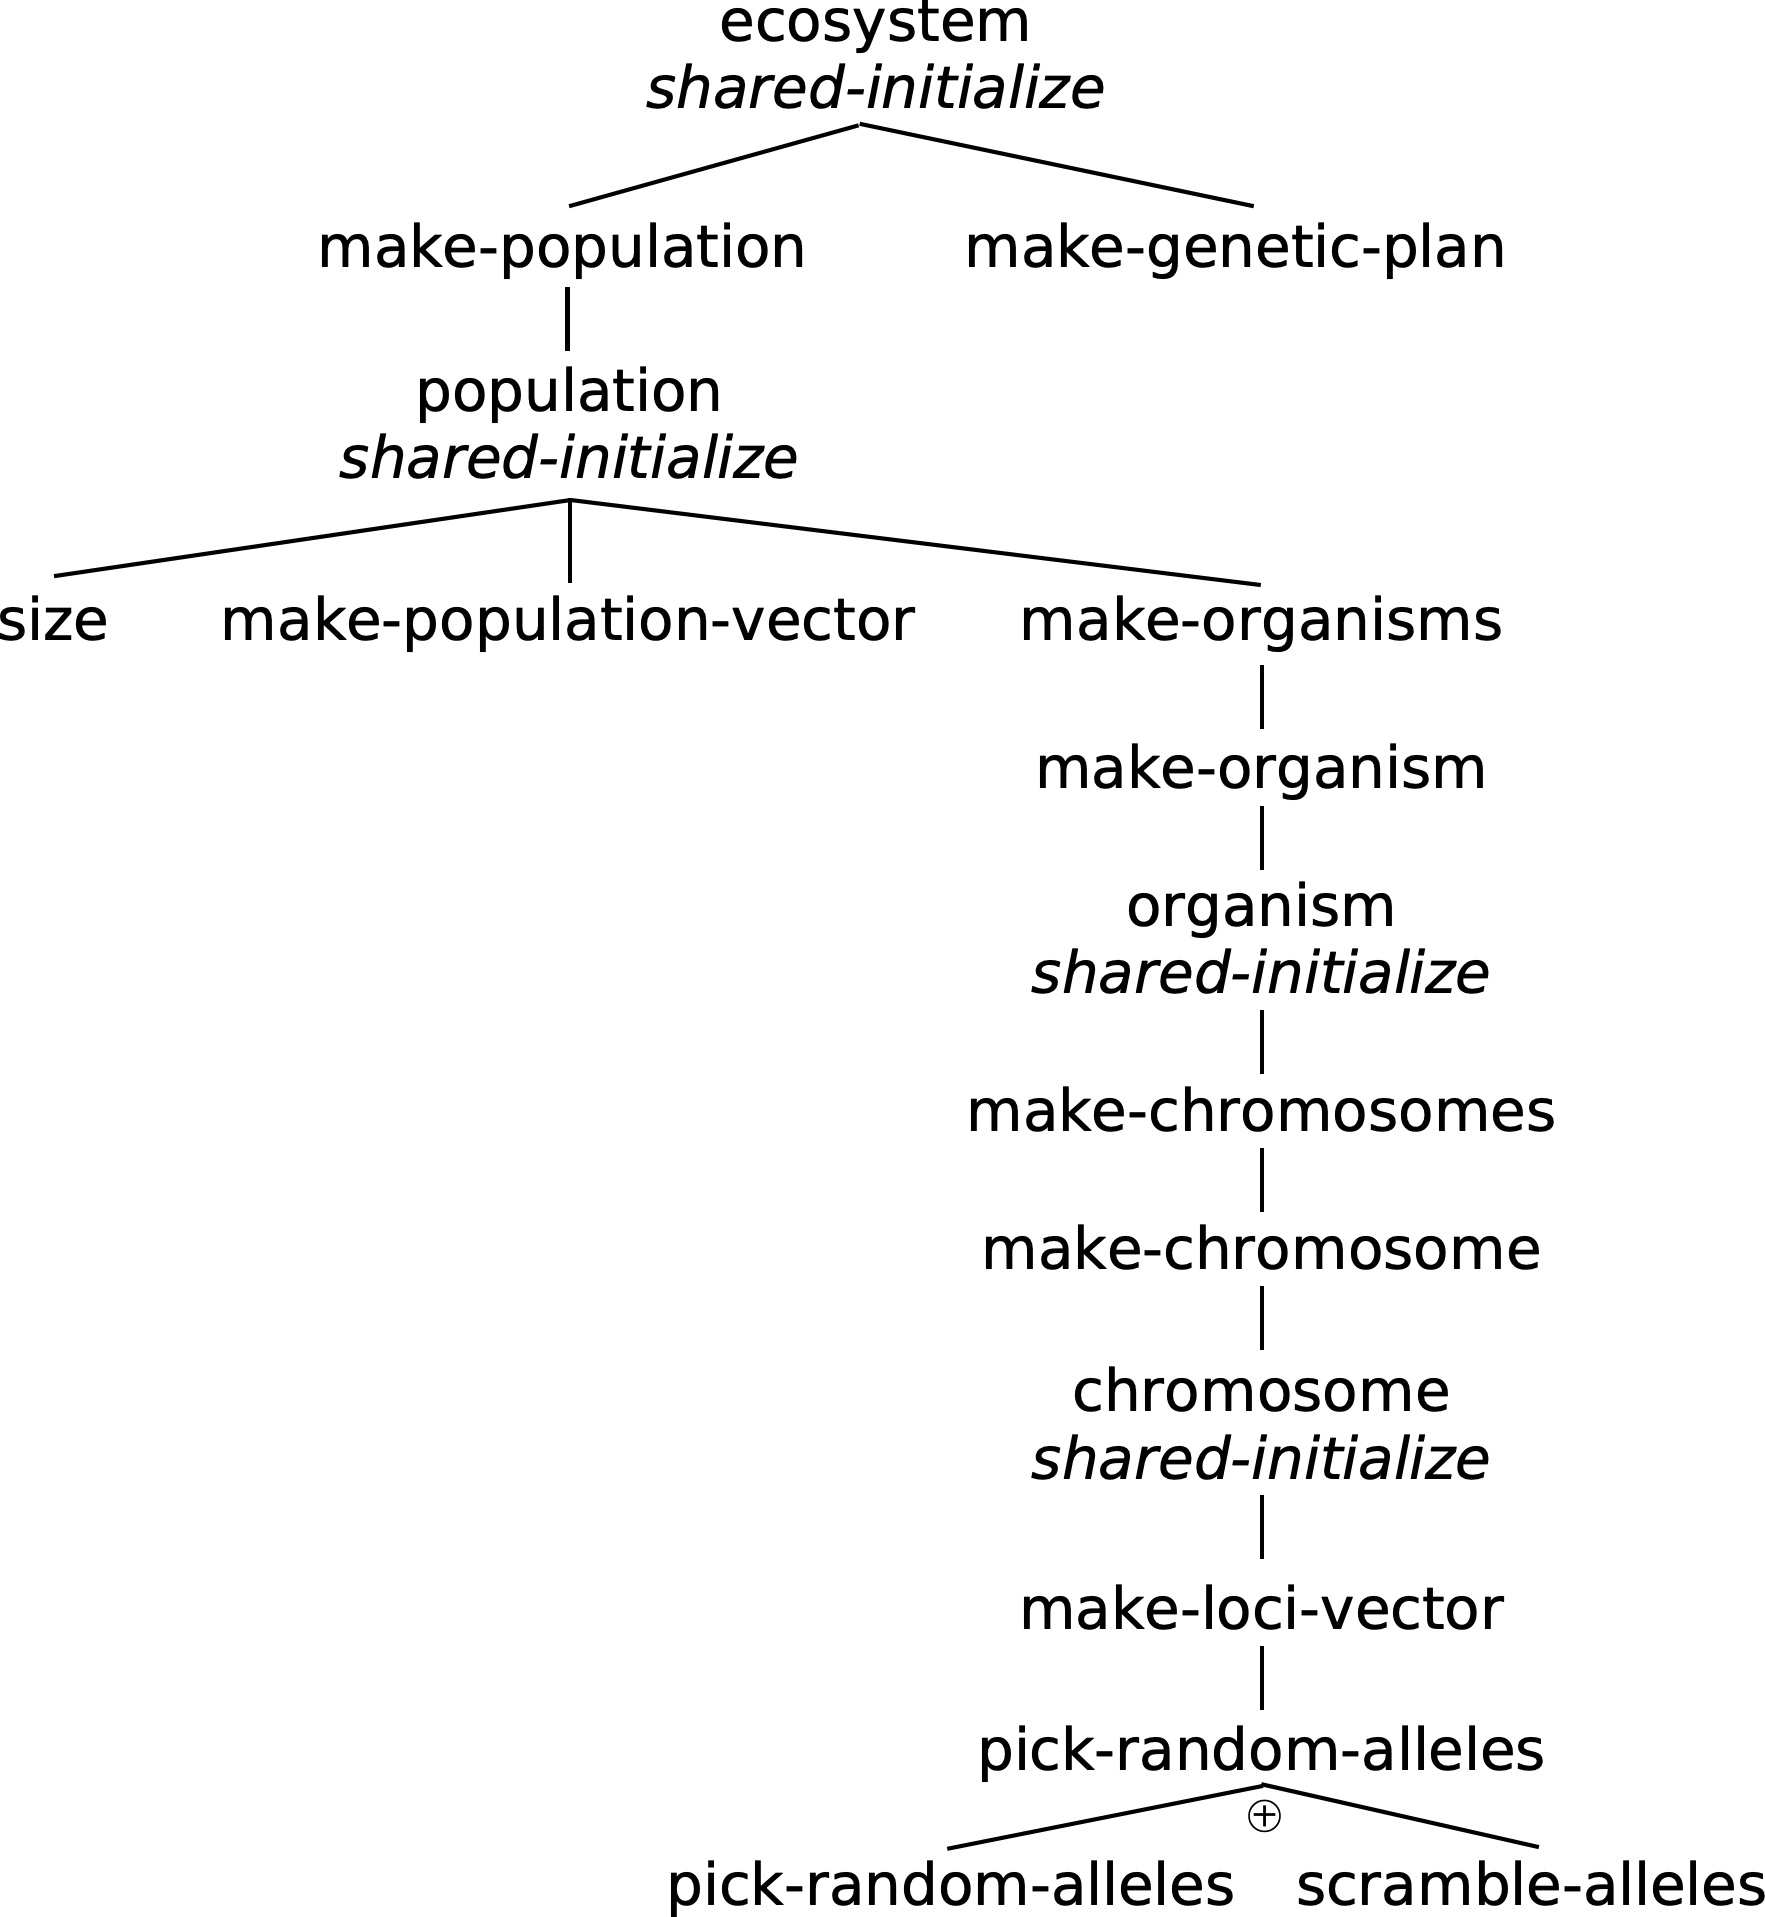
\includegraphics[width=\textwidth]{initialization-tree.eps}
  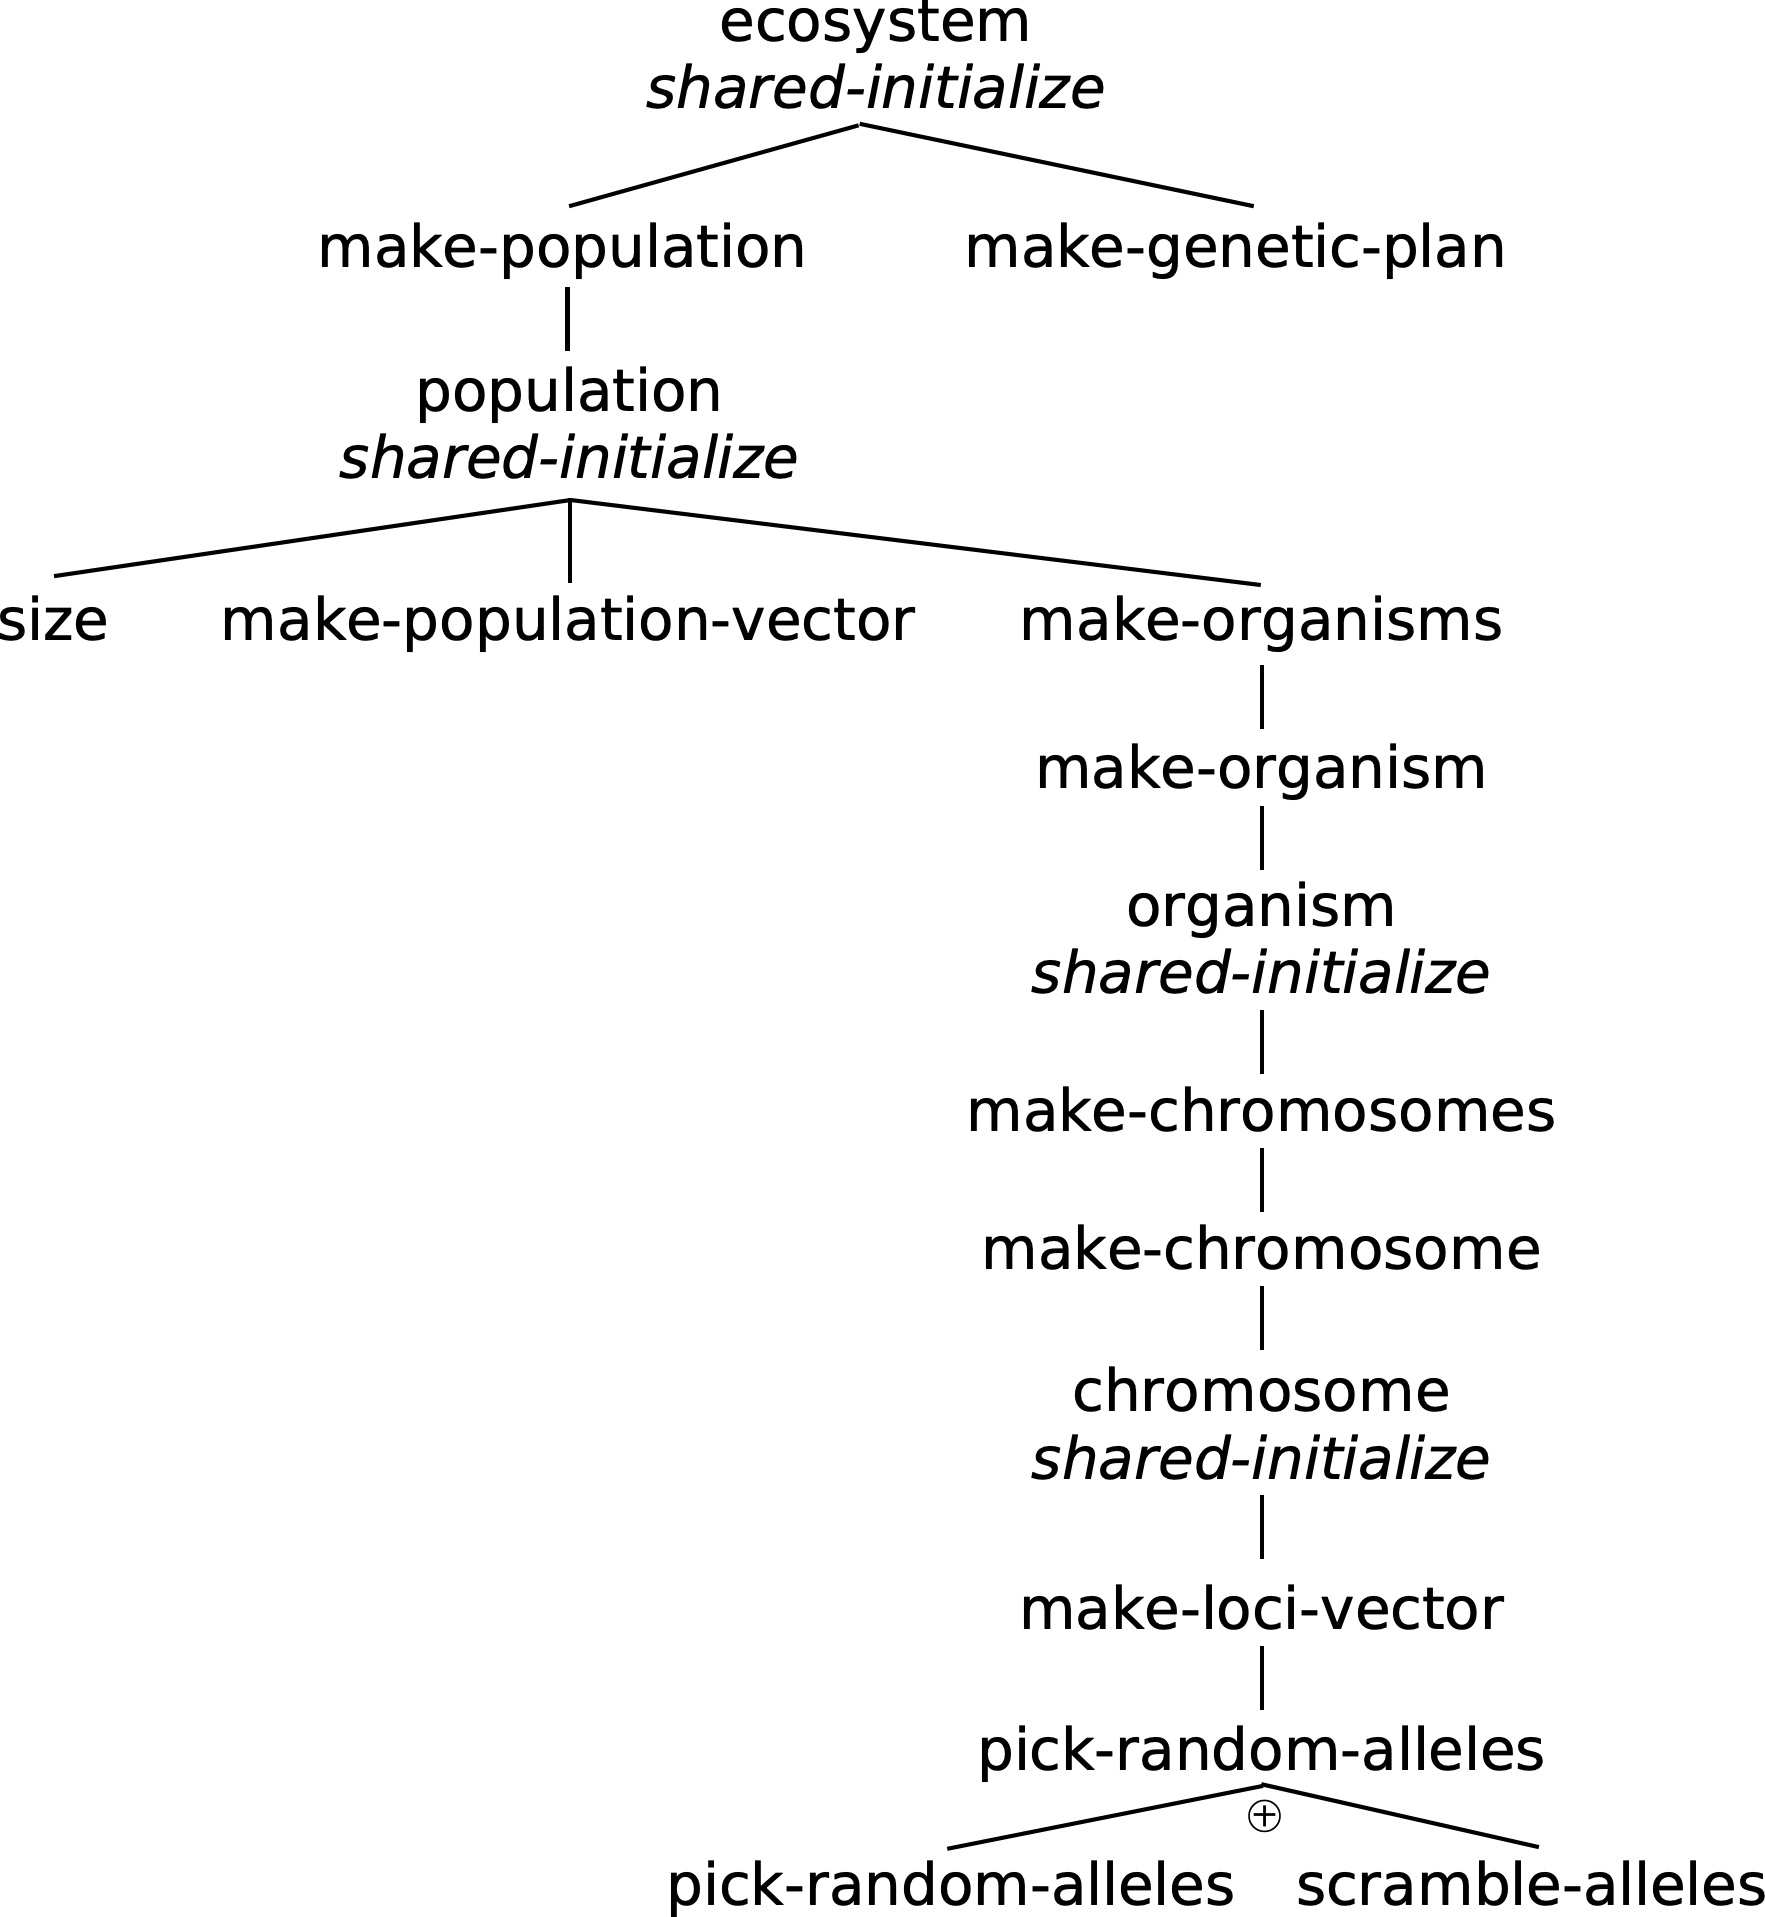
\includegraphics[width=0.6\textwidth]{initialization-tree.png}
  \caption{Call hierarchy for initialization of \Geco's principle structures}
  \label{fig:initialization-tree}
\end{figure}

\begin{figure}
  \centering
  % 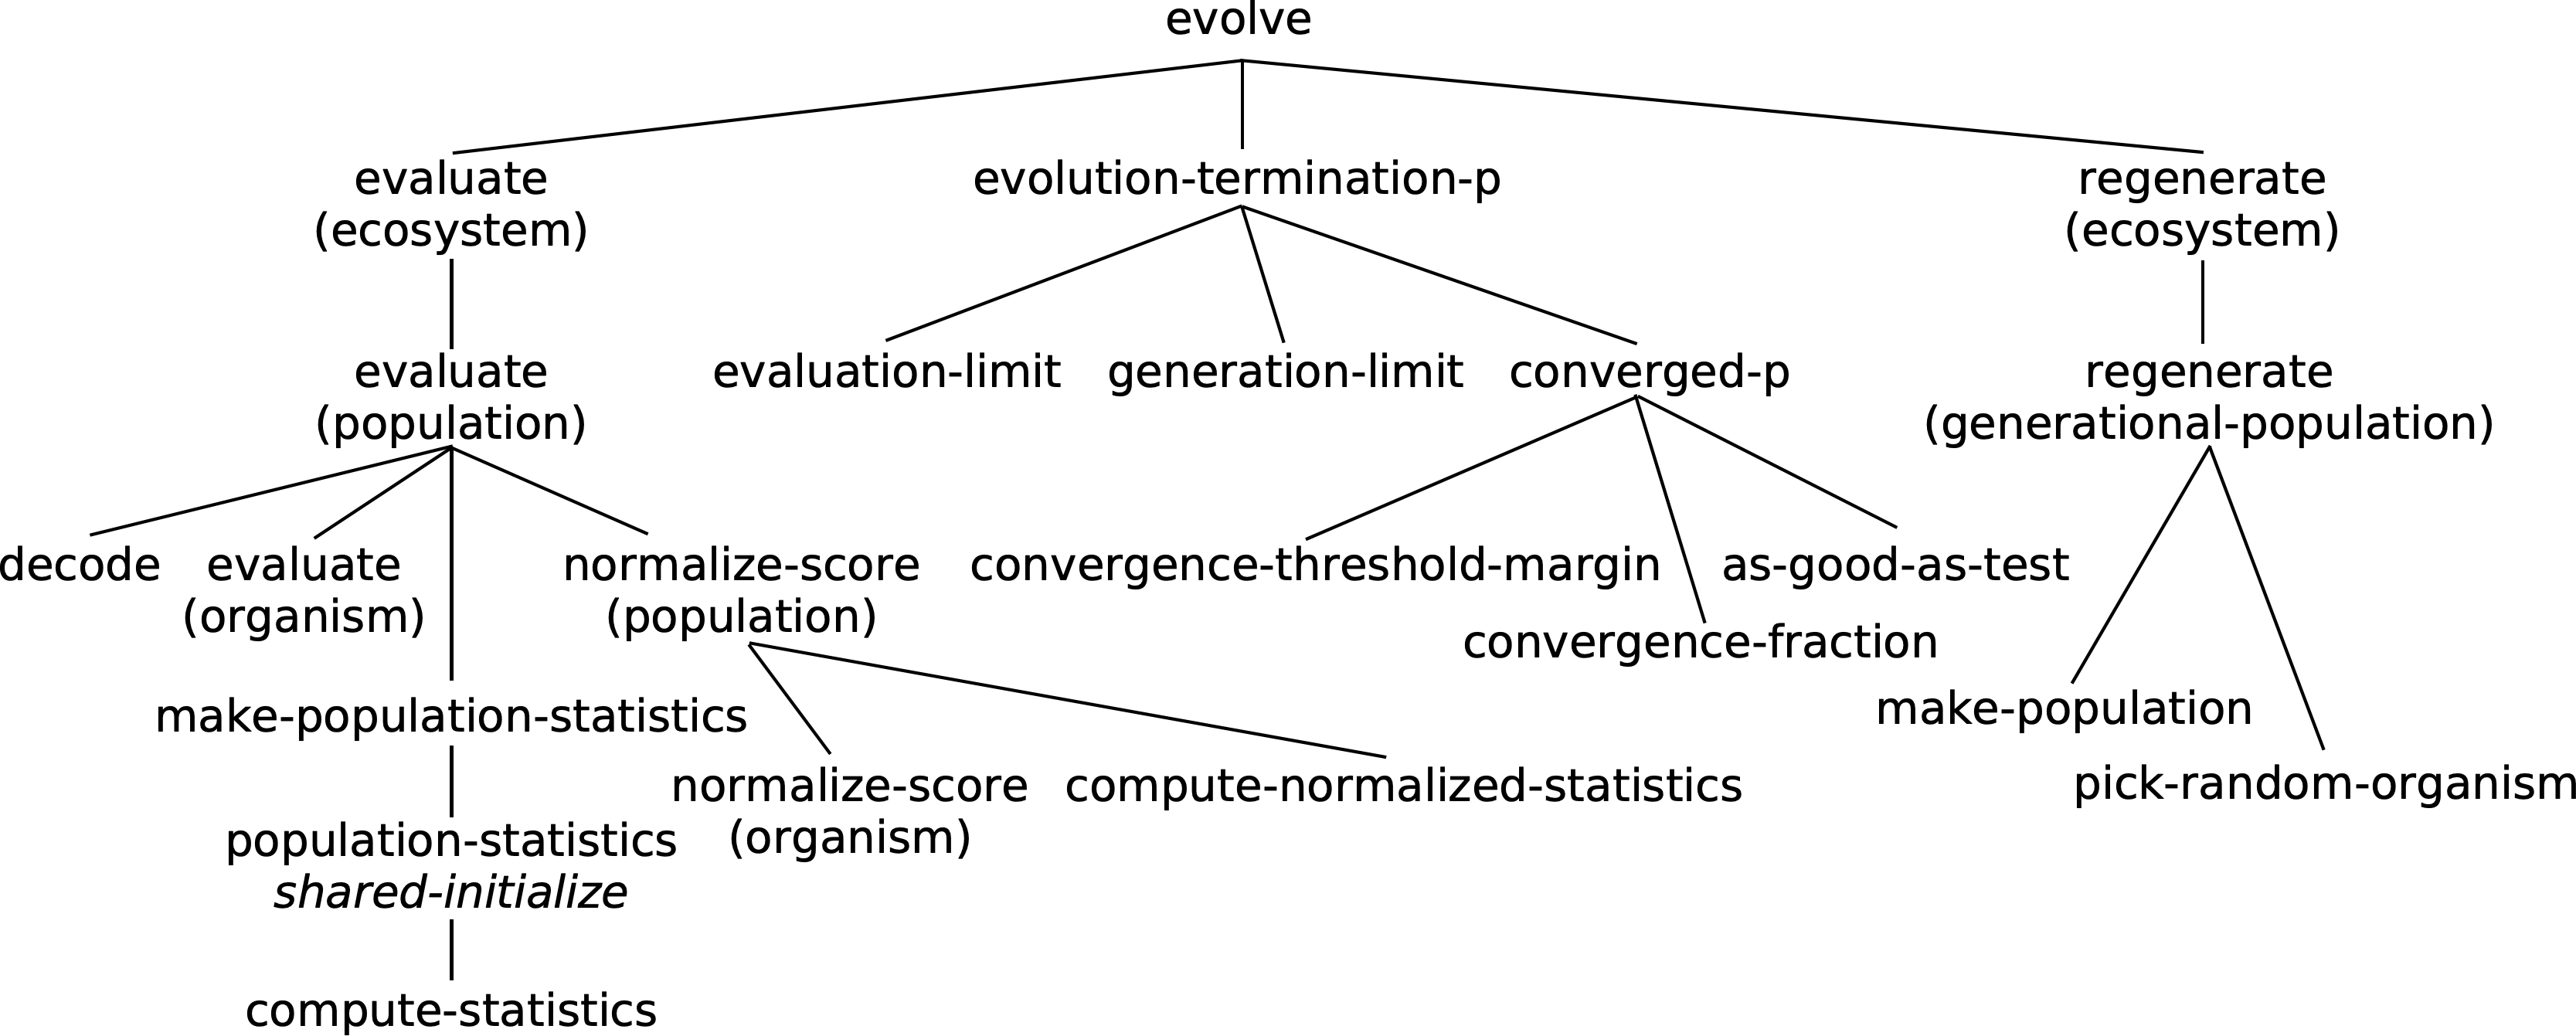
\includegraphics[width=\textwidth]{vert-evolve-tree.eps}
  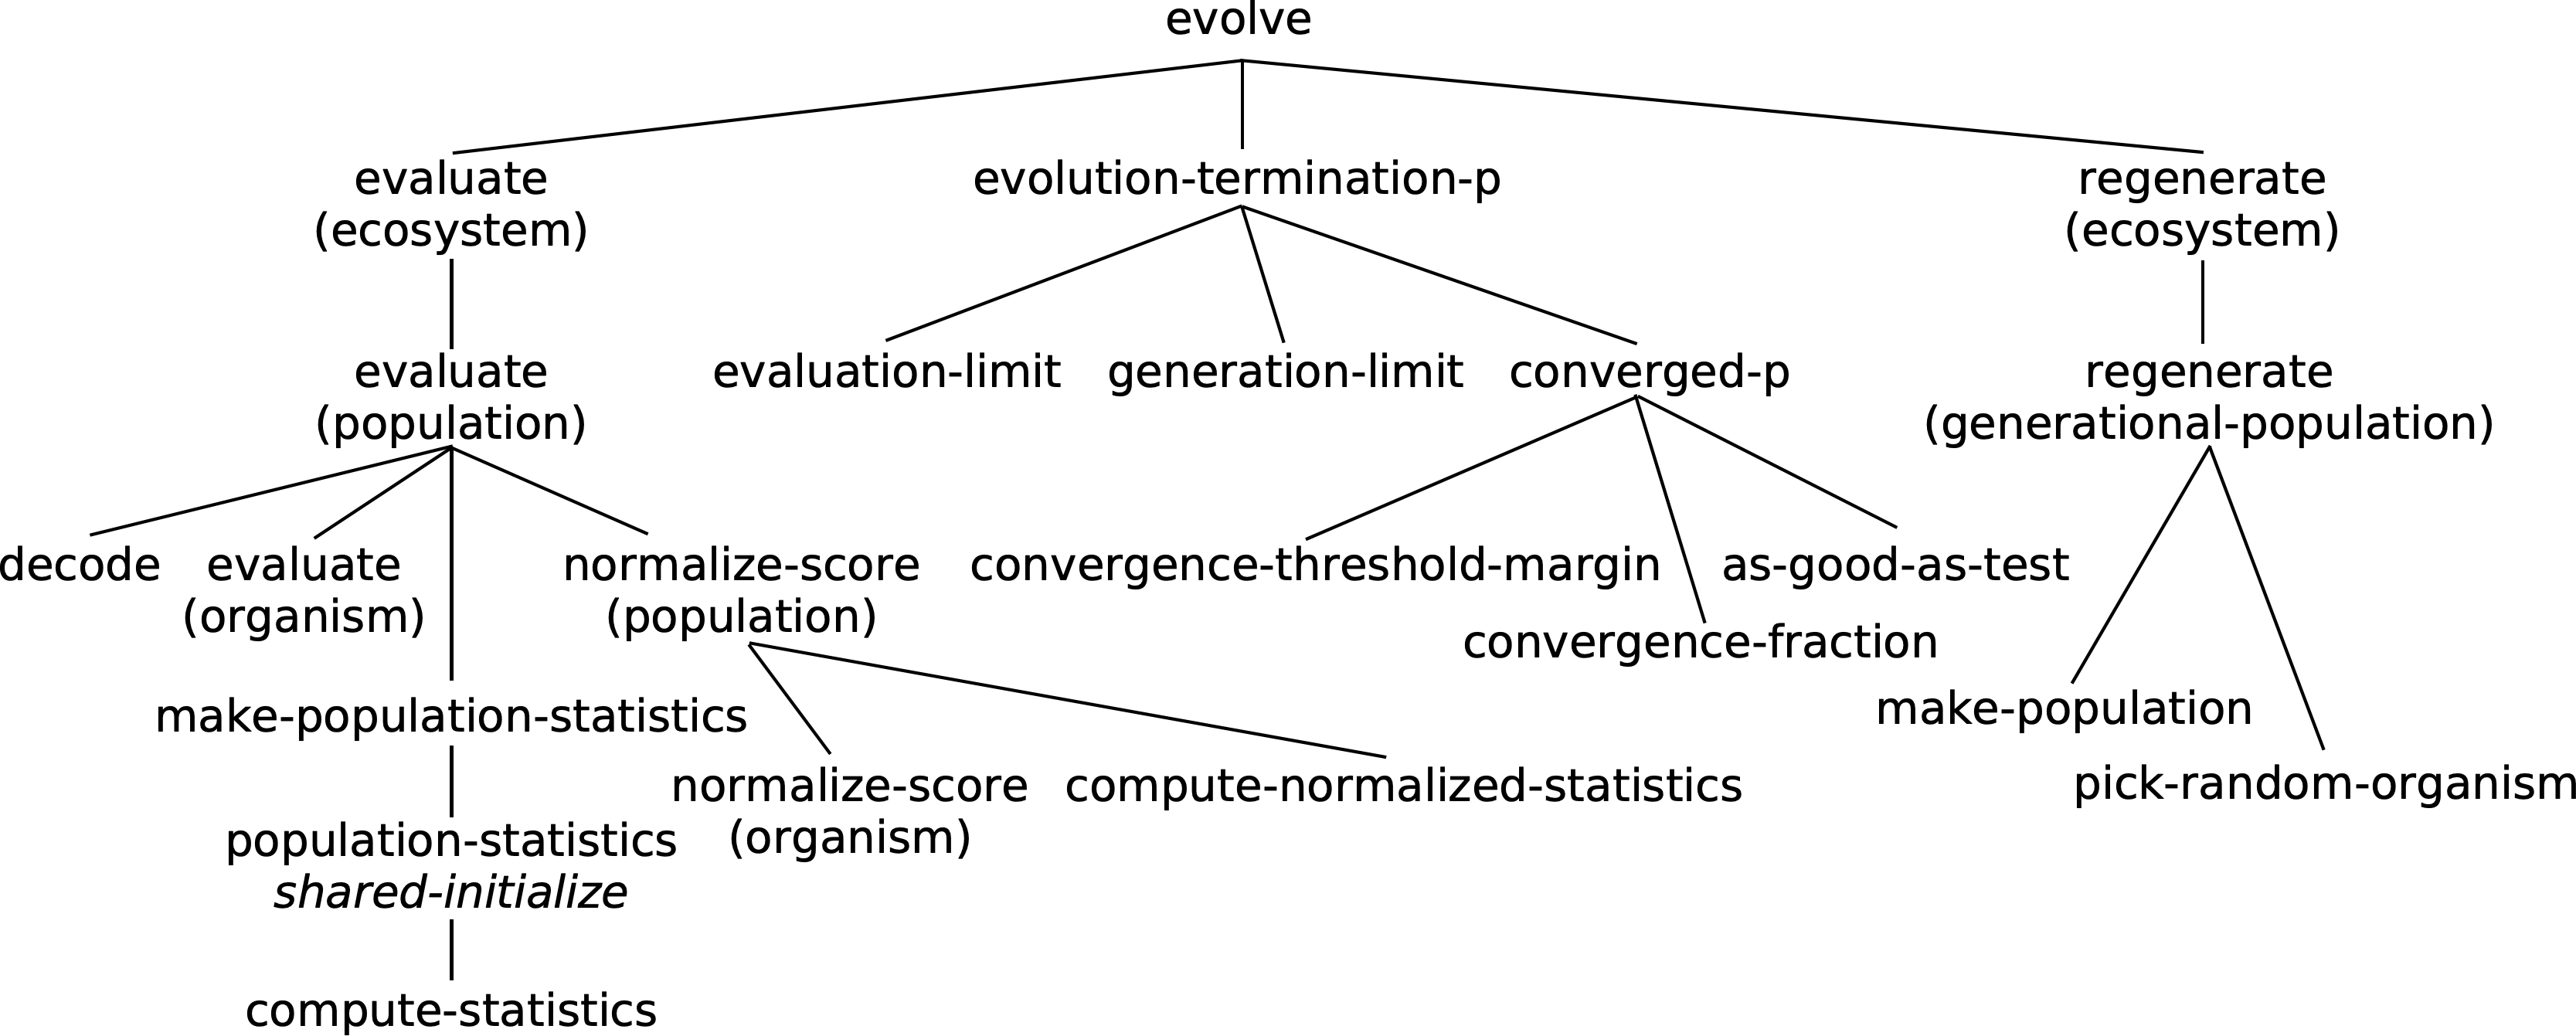
\includegraphics[width=\textwidth]{vert-evolve-tree.png}
  \caption{Call hierarchy for \Geco's evolutionary processing}
  \label{fig:evolve-tree}
\end{figure}

When supplied with the appropriate information, \geco\ can perform much of the
book-keeping, initialization, and control automatically.  This is made
possible by the built-in links between objects which are built upon the
\geco\ classes (see Figure~\ref{fig:class-interrelationships}).

\begin{figure}
  \centering	%% class-interrelationships.png is exported from class-interrelationships.pxd.pdf.cvd
  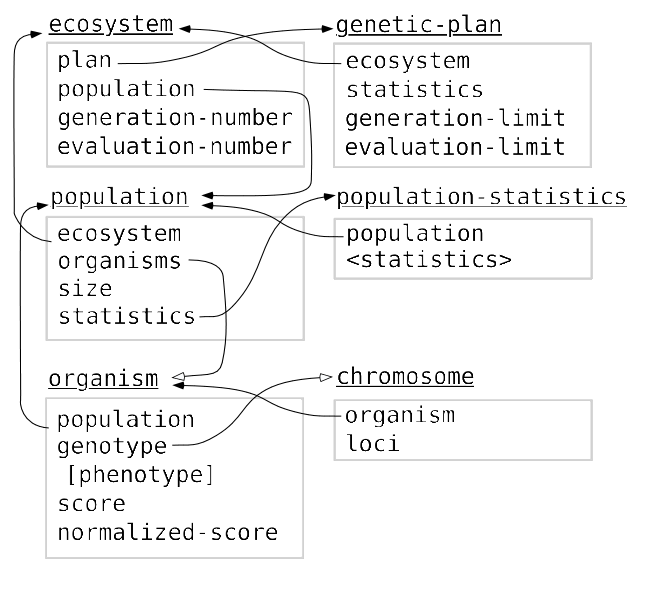
\includegraphics[width=0.75\textwidth]{class-interrelationships.png}
  % 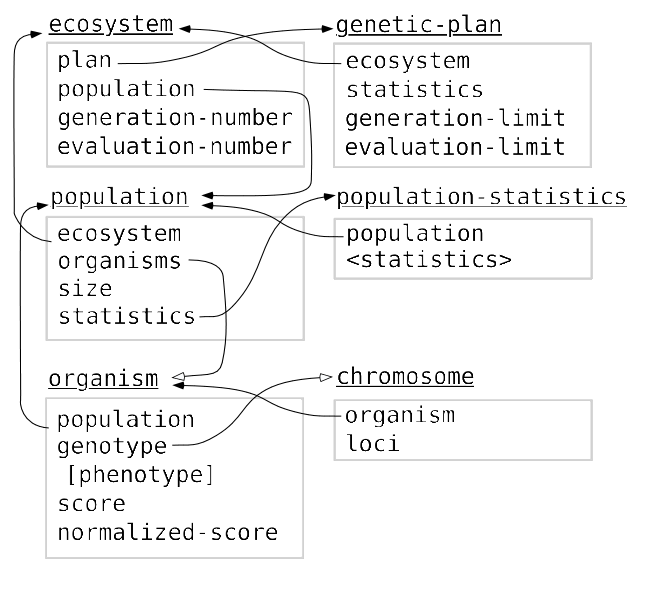
\includegraphics[]{class-interrelationships.png}
     \begin{center}
Solid head arrows indicate a one-to-one link;\\
hollow head arrows indicate a one-to-many link.
     \end{center}
  \caption{Interrelationships between \Geco\ objects}
  \label{fig:class-interrelationships}
\end{figure}



	% Copyright (C) 2020  George P. W. Williams, Jr.
\chapter{Details of GECO Classes and Functionality}

This chapter provides a more detailed discussion of each of \geco's 
classes, and the functionality implemented by their methods.   This functionality 
includes both the state retained by instances of each class (their {\em slots}),
and the functions (both generic and otherwise) which operate on those instances.

Even with all the functionality which \geco\ implements, it will still be
necessary to define some things which are specific to your application.
Generally this will be done by specializing \geco's classes (\ie, defining
some subclasses of \geco's builtin classes), and adding a few method
definitions to override and/or extend some of \geco's default behaviors.

Terminology Notes:

\begin{itemize}

\item In the material which follows, a statement which refers to `an instance of
\bold{a} {\it class-name} class' means that the instance is of the class
{\it class-name} or one of its subclasses. If the intent is to restrict the
instance to being of the named class, excluding subclasses, the wording will be
of the form `an instance of \bold{the} {\it class-name} class.'

\item In the descriptions of the methods, it will often be necessary to
distinguish between a generic function, a method for the generic function, and
the specific method supplied by \geco. A generic function and a method (as
specialized in the \term{flag line} above the description) are both parts of a
functional protocol which \geco\ expects to be honored.  A description
of a \geco-supplied method specifies that it
implements (fulfills) the requirements of this protocol.  \Geco\ may
define multiple methods (specialized for different classes) to implement
the generic function protocol for different classes.

\end{itemize}

For each class, the following sections will present the slots which 
are present in instances of the class (\ie, the values stored with each 
instance) and the functionality which has been defined for use with 
instances of the class (and its subclasses).
Generally, GAs implemented with \geco\ will not instantiate these classes.  
Instead, it will be more common to define subclasses which extend these 
classes (via added slots and methods) and specialize them (by overriding 
and/or extending inherited methods).


\section{The Ecosystem Class}

An \inxclass{ecosystem} is the highest level abstraction in a \geco\ implementation.
It is also the handle for manipulating a particular run of a GA. Since there may be
more than one instance of an \inxclass{ecosystem} in existence at one time, it is
possible to use \geco\ to create applications which use more than one GA at the same
time. The individual GAs could be competing, working on separate aspects of the same
problem, or they could be completely independent.
\filbreak
{\samepage

\Defclass {ecosystem}

\gap
\bold{Instance Allocated Slots}

  \Defslot {population}
  \defaccessor {population}

  An instance of a \inxclass{population} class.
  The population of an ecosystem is the set of organisms which are being 
  evolved.
\par}%end samepage

\filbreak

{\samepage
  \Defslotv {generation-number} {0}
  \defaccessor {generation-number}

  An integer, initially 0, which is 
  incremented each time the population enters a new {\em generation}.
  This happens each time the \inxgeneric{evolve}
  function is invoked on an \inxclass{ecosystem} instance (including
  \inxgeneric{evolve}'s recursive self-invocations). It should be noted
  that the actual creation of new members of the population (or creation
  of an entire new population) is expected to be handled by a \inxgeneric{regenerate}
  method specialized on a \inxclass{population} class, which
  is called by the default \geco-supplied \inxmethod{regenerate} method 
  specialized on \inxclass{ecosystem}.
\par}%end samepage

\filbreak

{\samepage
  \Defslotv {evaluation-number} {0}
  \defaccessor {evaluation-number}

  An integer, initially 0, which counts the number of times the 
  \inxgeneric{evaluate} function is applied to an \inxclass{organism} instance.
\par}%end samepage

\filbreak

{\samepage
  \Defslot {plan}
  \defaccessor {plan}

  An instance of a \inxclass{genetic-plan} class.
\par}%end samepage
\gap

\filbreak

The number of generations and evaluations are tracked by \geco\ so that the 
GA can be terminated based on the number of generations or evaluations 
exceeding some specific maximum limits, specified by the GA implementor.  
These limits are among the slots of the class \inxclass{genetic-plan}.

\filbreak
The \inxslot{population} and \inxslot{plan} are distinguished from the 
\inxclass{ecosystem} so that their classes may be specialized independently.  
Thus an instance of a single \inxclass{population} class may be manipulated 
using different \inxclass{plan}s, while instances of a single \inxclass{plan} may be 
used with different \inxclass{population}s.

\gap

\filbreak

{\samepage
	\bold{Instance Creation and Initialization}

The \inxclass{ecosystem} instance initialization has been extended by \geco\ by providing
a \cl{shared-initialize :AFTER} method for \inxclass{ecosystem}
to process the keyword arguments described below as follows:
\begin{itemize}
	\item If the call to \inxfun{make-instance}
	to create an instance of \inxclass{ecosystem} does not supply an initial population,
	then the \cl{:AFTER} method will initialize the \inxslot{population} slot using
	\inxgeneric{make-population}, with the values supplied via the \arg{:pop-class} and
	\arg{:pop-size} initargs.
	The call to \inxgeneric{make-population} also passes a value of \cl{t} for the \cl{:random}
	keyword argument, causing the initial population to be initialized to random organisms.
	(See Section~\ref{sec:population},
	page~\pageref{sec:population}.)
	
	\item Similarly, if a \inxclass{genetic-plan} instance is not supplied, then the \cl{:AFTER}
	method will initialize the \inxslot{plan} slot using \inxgeneric{make-genetic-plan}, with
	the value supplied via the \arg{:plan-class} initarg, and initializes the plan
	instance's \inxslot{generation-limit} and \inxslot{evaluation-limit} slots using the
	\arg{:gneration-limit} and \arg{:evaluation-limit} initargs. (See Section~\ref{sec:genetic-plan},
	page~\pageref{sec:genetic-plan}.)
\end{itemize}
The \inxgeneric{make-population} and \inxgeneric{make-genetic-plan} generic functions and
methods will be described subsequently, along with other \inxclass{ecosystem}-specialized
methods.
No special functions for the creation of \inxclass{ecosystem} instances have been defined,
since \inxgeneric{make-instance} and the standard \term{CLOS} protocol it follows provide all
the necessary functionality.

\par}%end samepage

\filbreak

{\samepage
\Definitarg {:plan-class}

  Provide the class for the \inxclass{genetic-plan} to be used by the
\inxclass{ecosystem}.
\par}%end samepage

\filbreak

{\samepage
\Definitarg {:pop-class}

  Provide the class for the \inxclass{population} instances to be created by
the \inxclass{ecosystem}.
\par}%end samepage

\filbreak

{\samepage
\Definitarg {:pop-size}

  Specifies the size to be used when the \inxclass{ecosystem} creates
\inxclass{population} instances.
\par}%end samepage

\filbreak

{\samepage
\Definitarg {:generation-limit}

This initarg is intended to specify the maximum number of generations which the ecosystem
will be allowed to evolve.
This limit is typically enforced by the \inxgeneric{evolution-termination-p} function
(see page~\pageref{evolution-termination-p}).
	
\par}%end samepage

\filbreak

{\samepage
\Definitarg {:evaluation-limit}

This initarg is intended to specify the maximum number of evaluations which the ecosystem
will be allowed to perform.
This limit is typically enforced by the \inxgeneric{evolution-termination-p} function
(see page~\pageref{evolution-termination-p}).

\par}%end samepage

\filbreak
\gap

{\samepage
\bold{Specialized Methods}

No special functions for the creation of \inxclass{ecosystem} instances have been defined
in \geco, since the \inxgeneric{make-instance} function and the standard \term{CLOS} protocol
it follows provide all the necessary functionality.
\par}% end \samepage

\filbreak

{\samepage

% use \Eggeneric so the CLOS generic isn't indexed
\Eggeneric shared-initialize {standard-object slot-names \rest initargs}
\defaftermethod shared-initialize {(ecosystem \inxclass{ecosystem}) slot-names \rest initargs
	\key :plan-class :pop-class :pop-size :generation-limit :evaluation-limit}

This method extends the initialization for \inxclass{ecosystem} instances to provide for the 
automatic creation and initialization of the \inxclass{population} and \inxclass{genetic-plan}
instances and slots.
The \inxgeneric{make-population} and \inxgeneric{make-genetic-plan} generic functions (described
next) are provided to support customization of these actions.
The call to \inxgeneric{make-population} in the default \geco-supplied method
passes a value of \cl{t} for the \cl{:random} keyword
argument, causing the initial population to be initialized to random organisms.
If \cl{:generation-limit} and \cl{evaluation-limit} are specified, the \inxslot{generation-limit}
and \inxslot{evaluation-limit} slots in the \inxclass{genetic-plan} instance are also initialized.
\par}% end \samepage

\filbreak

{\samepage

\Defgeneric make-population {ecosystem population-class \key :size :random}
\defmethod make-population {(ecosystem \inxclass{ecosystem}) population-class
	\key :size :random}
	\label{method:make-population}

This function provides an abstract interface to creation of a \inxclass{population} instance
to store in the \inxslot{population} slot of \arg{ecosystem}.
The primary \geco-supplied method
invokes \inxgeneric{make-instance} on the class \arg{population-class}, passing
the \arg{:size} argument, which determines the population size, and the
\arg{:random} argument, which if it is non-\cl{nil}, will cause the population to
be created with random organisms (intended for creation of the initial population).
It also returns the \inxclass{population} instance thus created.
\par}%end samepage

\filbreak

{\samepage
\Defgeneric make-genetic-plan {ecosystem genetic-plan-class}
\defmethod make-genetic-plan {(ecosystem \inxclass{ecosystem}) genetic-plan-class}
	\label{method:make-genetic-plan}

This function provides an abstract interface to creation of the \inxclass{genetic-plan}
instance for \arg{ecosystem}.  The \geco-supplied primary method invokes
\inxgeneric{make-instance} on \arg{genetic-plan-class}, and also supplies
\arg{ecosystem} so that the plan can be linked to the ecosystem (and vice-versa).
It also returns the \inxclass{genetic-plan} instance thus created.
\par}%end samepage

\filbreak

{\samepage
\Defgeneric evolve {ecosystem}
\defmethod evolve {(ecosystem \inxclass{ecosystem})}

This is the principle function which will be used by GA developers to invoke
their algorithm. The \geco-supplied primary method calls \inxmethod{evaluate} on
\arg{ecosystem}, and if the termination\index{termination} condition has not been
reached (see \inxgeneric{evolution-termination-p}), creates a new generation of
its \inxslot{population} via the \inxgeneric{regenerate} function, and
recurses to evolve some more\footnote{See the discussion in the footnote on
page~\pageref{recursive-vs-iterative-evolve}}.
The value returned by this function is not defined.
\par}%end samepage

\filbreak

{\samepage  
\Defgeneric evaluate {thing genetic-plan}
\defmethod evaluate {(ecosystem \cl{ecosystem}) genetic-plan}

The purpose of this function is to cause \arg{thing} to be evaluated according to
the specified \term{genetic plan}. The \geco-supplied primary method for
\inxclass{ecosystem} instances evaluates \arg{ecosystem} by calling
\inxgeneric{evaluate} on its \inxslot{population} with \arg{genetic-plan}. (Also
see the \inxmethod{evaluate} method specialized for the class \inxclass{population}, on
page~\pageref{evaluate-population}.)
The value returned by this function is not defined.
\par}%end samepage

\filbreak


\section{The Population Class} \label{sec:population}

A population is the most global structure upon which a GA operates. Although
\term{genetic operator}s are applied to the members (\term{organism}s in 
\geco's terminology, though they are often called
\ital{individuals}) of a population, it is at the level of the population that
the GA is really working.

\filbreak

{\samepage
\Defclass {population}

Instances of \inxclass{population} classes collect all the \inxclass{organism} 
instances of a generation.
\par}%end samepage

\gap

\filbreak

{\samepage
\bold{Instance Allocated Slots}

\Defslot {ecosystem}
\definitarg {:ecosystem}
\defaccessor {ecosystem}

Provides a link back to the \inxclass{ecosystem} instance to which the population belongs.
\par}%end samepage

\filbreak

{\samepage
\Defslot {organisms}
\defaccessor {organisms}

A vector, which contains all the \inxclass{organism} instances in the population.
\par}%end samepage

\filbreak

{\samepage
\Defslotv {size} {nil}
\definitarg {:size}
\defaccessor {size}

Either \cl{nil} or an integer, which indicates the size of the population, \ie,
the size of the vector in the \inxslot{organisms} slot. When \cl{nil}, the
organism vector will not be created automatically. \par}%end samepage

\filbreak

{\samepage
\Defslot {statistics}
\definitarg {:statistics}
\defaccessor {statistics}

An instance of a \inxclass{population-statistics} class, which holds statistics
\geco\ needs for the population. The \inxclass{population-statistics} class is
distinct from the \inxclass{population}class so that their sub-classes and methods may 
be specialized independently. 
\par}%end samepage

\gap
\filbreak

{\samepage

\bold{Instance Creation and Initialization}

The generic function \inxgeneric{make-population} (see page~\pageref{method:make-population})
is the \geco\ interface for creation of \inxclass{population} instances.

The initialization for instances of \inxclass{population} has been extended to
provide for automatic creation and initialization of the \inxslot{organisms}
vector. The functions \inxgeneric{make-organisms-vector} and
\inxgeneric{make-organisms} are used to permit customization of these
initialization actions; \inxgeneric{make-organisms-vector} is called when the
\inxslot{size} slot has a non-\cl{nil} value, and \inxgeneric{make-organisms} is
called only when both \inxslot{size} and \inxinitarg{:random} (below) have
non-\cl{nil} values. It is the responsibility of the \term{genetic plan} to
create the organisms after the initial generation.
\par}%end samepage

\filbreak

{\samepage
The \inxclass{population} instance initialization has been extended to support the following
additional initarg:

\Definitarg {:random}

The value of this keyword is passed to \inxgeneric{make-organisms}, and is intended
to support automatic initialization of the initial population to random organisms.
\par}%end samepage
\gap
  
\filbreak

{\samepage

\bold{Specialized Methods}

Note that most (if not all) of the generic functions in
Section~\ref{sec:selection-methods}, Selection Methods, have methods which
are specialized on the \inxclass{population} class.

\filbreak

{\samepage
	
% use \Eggeneric so the CLOS generic isn't indexed
\Eggeneric shared-initialize {standard-object slot-names \rest initargs}
\defaftermethod shared-initialize {(pop \inxclass{population}) slot-names \rest initargs
	\key :random}

This method extends the initialization for \inxclass{population} instances to provide for the 
automatic creation and initialization of the \inxclass{organism} instances for the population.
In the \geco-supplied default method, if the \inxslot{organisms} slot of 
\arg{pop} is unbound, the \inxgeneric{make-organisms-vector} generic function
(see below) is invoked to initialize the \inxslot{organisms}
slot; and then, if the \arg{:random} keyword argument is non-\cl{nil}, the
\inxgeneric{make-organisms} function (see below) is invoked to initialize
the population's organism vector to random organisms.
\par}% end \samepage

\filbreak

{\samepage
\Defgeneric make-organisms-vector {population size}
\defmethod make-organisms-vector {(population \inxclass{population}) size}

This function provides an abstract interface to creation of the population's
organisms vector (the vector which holds \arg{population}'s organisms). The
\arg{size} argument determines the size of the vector. The \geco-supplied primary
method uses the Common Lisp function \cl{make-array} to create an array of the
specified size.
It also returns the the array thus created.
\par}%end samepage

\filbreak

{\samepage
\Defgeneric make-organisms {population \key :random}
\defmethod make-organisms {(population \inxclass{population}) \key :random}

This function provides an abstract interface to creation of the organisms in
\arg{population}'s organisms vector. The \arg{:random} argument, when
non-\cl{nil}, causes all the new organisms to be random (\ie, have randomly
chosen chromosomes). The \geco-supplied primary method invokes
\inxgeneric{make-organism} for each position in the organisms vector. The
\arg{:random} argument is passed to each call to \inxgeneric{make-organism}.
The value returned by this function is not defined.
\par}%end samepage

\filbreak

{\samepage
\Defgeneric make-organism {population \key :random :no-chromosome}
\defmethod make-organism {(population \inxclass{population}) \key :random :no-chromosome}
	\label{method:make-organism}

This function provides an abstract interface to creation of a single organism
based on the \inxgeneric{organism-class} of \arg{population}. The \arg{:random}
argument, when non-\cl{nil}, causes the new organism to be random (\ie, have
randomly chosen chromosomes). The \arg{:no-chromosome} argument, when
non-\cl{nil}, causes the organism to be created without chromosomes, avoiding
wasted work when the chromosomes will be supplied by other mechanisms, \eg,
\term{genetic operator}s. The \geco-supplied primary method passes \arg{population} to
the call to \inxgeneric{make-instance} so that the organism can have a back-link
to the population to which it belongs. The \arg{:random} and
\arg{:no-chromosomes} arguments are passed to \inxgeneric{make-instance}.
It also returns the the \inxclass{organism} instance thus created.
\par}%end samepage

\filbreak

{\samepage
\Defgeneric organism-class {population}

This function returns the class to be used to create organisms which will become members
of \arg{population}. The GA developer {\em must implement the primary method} for all
subclasses of the class \inxclass{population}. \Geco\ does not provide a default primary method
specialized on the \inxclass{population} class.\footnote{There are comments at the beginning
of the {\tt generics.lisp} file which summarize the functions which should or must be
defined to implement a working GA using \geco.}
\par}%end samepage

\filbreak

{\samepage
\Defgeneric evaluate {thing genetic-plan}
\defmethod evaluate {(population \inxclass{population}) (genetic-plan \inxclass{genetic-plan})}
\label{evaluate-population}

This function evaluates \arg{thing} according to \arg{genetic-plan}. This method
assures that each organism in \arg{population} is evaluated. The \geco-supplied
primary method only calls \inxgeneric{evaluate} on an organism if the organism
doesn't already have a \term{score} in its \inxslot{score} slot. After
\arg{population} has been evaluated, \inxgeneric{normalize-score} and
\inxgeneric{make-population-statistics} are called to assure that normalized
scores and statistics have been computed for the population.
The value returned by this function is not defined.
\par}%end samepage

\filbreak

{\samepage
\Defgeneric make-population-statistics {population}
\defmethod make-population-statistics {(population \inxclass{population})}
	\label{method:make-population-statistics}

This function provides an abstract interface to creation of the
\inxclass{population-statistics} instance for \arg{population}, based on the
\inxgeneric{population-statistics-class} of \arg{population}. The \geco-supplied
primary method passes \arg{population} to \inxgeneric{make-instance} so that the instance can
have a back-link to the population to which it belongs.
It also returns the \inxclass{population-statistics} instance thus created.
\par}%end samepage

\filbreak

{\samepage
\Defgeneric compute-statistics {population}
\defmethod compute-statistics {(population \inxclass{population})}

This function provides an abstract interface for computing statistics for
\arg{population}. This method provieds a place for a population class to provide
for customization of statistics computation. The \geco-supplied primary method
simply calls \inxgeneric{compute-statistics} on the statistics instance of
\arg{population}. (Also see the description of \inxmethod{compute-statistics}
on page~\pageref{compute-population-statistics},
specialized on the class \inxclass{population-statistics}, and
Section~\ref{sec:pop-stats-class}, which details the statistics that are computed.)
The value returned by this function is not defined.
\par}%end samepage

\filbreak

{\samepage
\Defgeneric compute-binary-allele-statistics {population}
\defmethod compute-binary-allele-statistics {(population \inxclass{population})}

This function returns a list of vectors (one per binary chromosome in the
organisms of \arg{population}) of counts (\cl{fixnum}s), by locus, of non-zero
alleles. For example, if the organisms in a population contain $c$ binary
chromosome (and any number of non-binary chromosomes), and each binary chromosome
contains $b$ loci, then this function will return a list containing $c$ vectors
of $b$ fixnums. Each \cl{fixnum} in the returned vectors is a count of non-zero
alleles in the entire population at the locus whose index corresponds to the
index into the $c^{\rm th}$ vector of counts. \Eg, if the third count in the
first vector is 7, then the entire population contains 7 non-zero alleles in
locus 3 of the first binary chromosome of each organism.
\par}%end samepage

\filbreak

{\samepage
\Defgeneric normalize-score {thing plan}
\defmethod normalize-score {(population \inxclass{population})
                            \hbox{(genetic-plan \inxclass{genetic-plan})}}

This function computes the normalized
\term{score}(s)\index{score!normalization}\index{normalization} for \arg{thing}.
This method computes the normalized scores for all organisms in \arg{population}.
The \geco-supplied primary method for \inxclass{population} invokes
\inxgeneric{normalize-score} (see page \pageref{method:normalize-score:organism})
for each organism in \arg{population}, according to the \arg{genetic-plan}, and
updates \cl{(statistics \arg{population})} with normalized values using the function
\inxgeneric{compute-normalized-statistics}.
The value returned by this function is not defined.

[Note that \geco\ version 2.1 changed the calling sequence for this generic function and all its methods.]
\par}%end samepage

\filbreak

There are a number of different ways to normalize\index{normalization} the
scores. With some plans and evaluation functions, it may not even be necessary,
though beware that the score should always be $\ge 0$ (see Chapter 4 of
\cite{ga:goldberg}, under the sections on Scaling Mechanisms and Ranking
Procedures).

\filbreak

{\samepage
\Defgeneric population-statistics-class {population}
\defmethod population-statistics-class {(population \inxclass{population})}

This function returns the population-statistics class which will be used for
\arg{population.} The \geco-supplied primary method specialized for the
\inxclass{population} class returns \inxclass{population-statistics}.
\par}%end samepage

% This function could be performed by \cl{:allocation :per-class} slots 
% if and when they can be implemented portably in Common Lisp.

\filbreak

{\samepage
\Defgeneric converged-p {population}
\defmethod converged-p {(population \inxclass{population})}
	\label{population:converged-p}
This function is a predicate which indicates whether \arg{population} has
\concept{converged}, which is useful as a termination\index{termination}
condition. The \geco-supplied primary method defines convergence as
either of the following:
\par}%end samepage

\filbreak

{\samepage
  \begin{enumerate}
    \item All organisms in \arg{population} have the same \inxslot{score}; or
    \item At least a portion of \arg{population} (specified by the
        \inxgeneric{convergence-fraction} function) has a 
        \inxslot{normalized-score} which is {\em as good as} the value specified by the
        \inxgeneric{convergence-threshold-margin} function.
  \end{enumerate}
}%end samepage

\filbreak

Note that this allows \geco\ to either {\em maximize} or {\em minimize}
\term{scores}. The mechanism for determining whether \geco\ maximizes or minimizes,
and hence how it determines {\em as good as} or {\em better than}, is determined by
mixing one of two classes with the population class used by the GA. These
\term{mixin classes} are described below, in section
\ref{sec:population-mixin-classes}.

\filbreak

{\samepage
\subsection{Subclasses of Population}

\Defclassv {generational-population} {population}

This class is a subclass of \inxclass{population} which provides explicit support
for the `standard' generational style of GA. The class has no
slots, but methods described elsewhere specialize on this class (see
\inxmethod{regenerate}, page~\pageref{method:regenerate}).
\par}%end samepage
\filbreak

Eventually \geco\ may contain support for other styles of population handling,
possibly including parallel sub-populations, steady-state populations, \etc.

\gap
\filbreak

{\samepage
\bold{Instance Creation and Initialization}

The generic function \inxgeneric{make-population} (see
page~\pageref{method:make-population}) is the \geco\ interface for creation
of instances of \inxclass{population} and its subclasses.
\par}%end samepage

\filbreak

{\samepage
\subsection{Population Mixin Classes}	\label{sec:population-mixin-classes}

\Defclass {maximizing-score-mixin}
\defclass {minimizing-score-mixin}

Neither of these classes has any slots or has special provisions for
instance creation or initialization.
\par}%end samepage

\gap

\filbreak

{\samepage

\bold{Specialized Methods}

Both classes implement methods for the following generic functions:

\Defgeneric maximizing-p {population}
\defmethod maximizing-p {(population \inxclass{maximizing-score-mixin})}
\defmethod maximizing-p {(population \inxclass{minimizing-score-mixin})}
\Defgeneric minimizing-p {population}
\defmethod minimizing-p {(population \inxclass{maximizing-score-mixin})}
\defmethod minimizing-p {(population \inxclass{minimizing-score-mixin})}

These functions permit algorithms to efficiently determine whether the
\arg{population} is minimizing or maximizing.  The \geco-supplied methods
return either \cl{t} or \cl{nil} as appropriate for their class.
\par}%end samepage

%These functions could all be performed by \cl{:allocation :per-class} slots if
%and when they can be implemented portably in Common Lisp.

\filbreak

{\samepage
\Defgeneric convergence-fraction {population}
\defmethod convergence-fraction {(population \inxclass{maximizing-score-mixin})}
\defmethod convergence-fraction {(population \inxclass{minimizing-score-mixin})}

This function returns the convergence-fraction value which should be used for
\arg{population} by the \inxgeneric{converged-p} function. The \geco-supplied
primary methods for both the \inxclass{maximizing-score-mixin} and the
\inxclass{minimizing-score-mixin} classes return $0.95$. These values are not
necessarily the {\em right} numbers in any real sense, but they are probably
reasonable for many applications. Some applications may want to provide different
values, and possibly even adaptive methods for specialized subclasses.
\par}%end samepage

\filbreak

{\samepage
\Defgeneric convergence-threshold-margin {population}
\defmethod convergence-threshold-margin {(population \inxclass{maximizing-score-mixin})}
\defmethod convergence-threshold-margin {(population \inxclass{minimizing-score-mixin})}

This function returns the convergence-threshold-margin value which should be used
for \arg{population} by the \inxgeneric{converged-p} function. The \geco-supplied
primary method provided for the \inxclass{maximizing-score-mixin} class returns
$0.95$, and the method provided for the \inxclass{minimizing-score-mixin} class
returns $0.05$. These values are not necessarily the {\em right} numbers in any real
sense, but they are probably reasonable for many applications. Some applications may
want to provide different values, and possibly even adaptive methods for specialized
subclasses. 
\par}%end samepage

\filbreak

{\samepage
\Defgeneric as-good-as-test {population}
\defmethod as-good-as-test {(population \inxclass{maximizing-score-mixin})}
\defmethod as-good-as-test {(population \inxclass{minimizing-score-mixin})}

This function returns a function of two numeric arguments, which when applied to
\inxslot{score}s from organisms in \arg{population}, indicates whether or not the first
score is as good as the second. The \geco-supplied primary method for the
\inxclass{maximizing-score-mixin} class returns \cl{#'>=}, and the method provided
for the \inxclass{minimizing-score-mixin} class returns \cl{#'<=}.
\par}%end samepage

\filbreak

{\samepage
\Defgeneric better-than-test {population}
\defmethod better-than-test {(population \inxclass{maximizing-score-mixin})}
\defmethod better-than-test {(population \inxclass{minimizing-score-mixin})}

This function returns a function of two numeric arguments, which when applied to
\inxslot{scores} from organisms in \arg{population}, indicates whether or not the first
score is better than the second. The \geco-supplied primary method provided
for the \inxclass{maximizing-score-mixin} class returns \cl{#'>}, and the method
provided for the \inxclass{minimizing-score-mixin} class returns \cl{#'<}.
\par}%end samepage

\filbreak

{\samepage
\Defgeneric best-organism {population}
\defmethod best-organism {(population \inxclass{maximizing-score-mixin})}
\defmethod best-organism {(population \inxclass{minimizing-score-mixin})}

This function returns the best organism in the corresponding population from
population statistics of \arg{population}. The \geco-supplied primary method for the
\inxclass{maximizing-score-mixin} class uses \inxgeneric{max-organism}, and the method
provided for the \inxclass{minimizing-score-mixin} class uses \inxgeneric{min-organism}.
\par}%end samepage

\filbreak

{\samepage
\Defgeneric worst-organism {population}
\defmethod worst-organism {(population \inxclass{maximizing-score-mixin})}
\defmethod worst-organism {(population \inxclass{minimizing-score-mixin})}

This function returns the best organism in the corresponding population from
population statistics of \arg{population}. The \geco-supplied primary method for the
\inxclass{maximizing-score-mixin} class uses \inxgeneric{min-organism}, and the method
provided for the \inxclass{minimizing-score-mixin} class uses \inxgeneric{max-organism}.
\par}%end samepage

\filbreak

{\samepage
\Defgeneric best-organism-accessor {population}
\defmethod best-organism-accessor {(population \inxclass{maximizing-score-mixin})}
\defmethod best-organism-accessor {(population \inxclass{minimizing-score-mixin})}

This function returns a function which can be applied to an instance of the
\inxclass{population-statistics} class of \arg{population} to obtain the best organism in the
corresponding population. The \geco-supplied primary method for the
\inxclass{maximizing-score-mixin} class returns \cl{#'}\inxgeneric{max-organism},
and the method provided for the \inxclass{minimizing-score-mixin} class returns
\cl{#'}\inxgeneric{min-organism}.
\par}%end samepage \filbreak

\filbreak

{\samepage
\Defgeneric worst-organism-accessor {population}
\defmethod worst-organism-accessor {(population \inxclass{maximizing-score-mixin})}
\defmethod worst-organism-accessor {(population \inxclass{minimizing-score-mixin})}

This function returns a function which can be applied to an instance of the
\inxclass{population-statistics} class of \arg{population} to obtain the worst organism in
the corresponding population. The \geco-supplied primary method for the
\inxclass{maximizing-score-mixin} class returns \cl{#'}\inxgeneric{min-organism}, and the
method provided for the \inxclass{minimizing-score-mixin} class returns
\cl{#'}\inxgeneric{max-organism}. \par}%end samepage \filbreak


\section{The Organism Class}

An \concept{organism} is a member of the population which is being evolved by the GA. Typically
an organism represents a single distinct solution to the problem which the GA is set to
solve, although sometimes\footnote{%
%
In some kinds of Learning Classifier Systems \cite{gbml:holland-reitman,gbml:holland-induction},
the so-called `Michigan' approach (for the University of Michigan), each member of a
population represents a rule, and the entire population cooperatively evolves as a ruleset.
By way of contrast, in the `Pitt' approach (for the University of Pittsburg) each member of a
population represents an entire ruleset.
%
} an entire population of organisms cooperate to constitute a solution.
\filbreak

In \geco, an instance of an organism class is a collection of information related to
a population member. This may include an explicit representation of the population
member (the organism's \term{phenotype}), or a coded representation (the
\term{genotype}), or both. An evaluation of the organism (its \term{score}) is also
present, so that the GA can have some way to determine which organisms are better
than others, and to what extent.
\filbreak

Typically, during the operation of the GA, the \term{genetic operator}s
manipulate the organism's genotype, and then that is converted into the
phenotype, which is then evaluated to produce a score. The genotype typically
consists of one or more \term{chromosomes}, which encode the features of the
phenotype. In some GAs the genotype is bypassed, and the \term{genetic operator}s
manipulate the phenotype directly, in which case the genotype is empty. In other
GAs, the organism's score can be determined directly from the genotype, and the
conversion from genotype to phenotype is completely omitted. The phenotype is not
included in the basic \inxclass{organism} class, but as a mixin described later (see
\inxclass{organism-phenotype-mixin}, page~\pageref{class:organism-phenotype-mixin}).

\Defclass {organism}

\filbreak

{\samepage

\gap

\bold{Instance Allocated Slots}

  \Defslotv {population} {nil}
  \definitarg {:population}
  \defaccessor {population}

  Provides a link back to the population to which the organism belongs.
\par}%end samepage

\filbreak
{\samepage
  \Defslotv {genotype} {nil}
  \definitarg {:genotype}
  \defaccessor {genotype}

  A list of zero or more chromosomes, which form an encoded representation
  of the organism. 
\par}%end samepage

\filbreak
{\samepage
  \Defslotv {score} {nil}
  \definitarg {:score}
  \defaccessor {score}

  A (raw) numeric representation of the value of the organism to the GA,
  or (initially) \cl{nil}, indicating that the organism hasn't been evaluated.
\par}%end samepage

\filbreak
{\samepage
  \Defslotv {normalized-score} {nil}
  \definitarg {:normalized-score}
  \defaccessor {normalized-score}

  A normalized version of \inxslot{score}, with respect to the rest of the
population, or \cl{nil}, indicating that the organism either hasn't been
evaluated, or that the scores haven't been normalized.
\par}%end samepage

\gap

\filbreak
{\samepage

\bold{Instance Creation and Initialization}

The generic function \inxgeneric{make-organism} (see page~\pageref{method:make-organism})
is the \geco\ interface for creation of \inxclass{organism} instances.

The initialization for instances of \inxclass{organism} has been extended to
support the following additional initargs:

\Definitarg {:random}

The initialization for organism instances has also been extended to check the
\inxslot{genotype} slot, and if it is null it will create chromosomes for the
organism, using the \inxgeneric{make-chromosomes} function, passing the value of the
\arg{:random} keyword argument. This is intended to support automatic initialization
of the initial population. 
\par}%end samepage

\filbreak
{\samepage
\Definitarg {:no-chromosomes}

When non-\cl{nil}, this initarg suppresses creation of the new
organism's chromosomes.
\par}%end samepage

\gap

\filbreak
{\samepage

\bold{Specialized Methods}

{\samepage
	
% use \Eggeneric so the CLOS generic isn't indexed
\Eggeneric shared-initialize {standard-object slot-names \rest initargs}
\defaftermethod shared-initialize {(organism \inxclass{organism}) slot-names \rest initargs
	\key :random :no-chromosomes}

This method extends the initialization for \inxclass{organism} instances to provide for the 
automatic creation and initialization of the \inxclass{chromosome} instances for the organism.
In the \geco-supplied default method, the \inxgeneric{make-chromosomes} generic function
(see page~\pageref{method:make-chromosomes}) is invoked unless the \inxslot{genotype} slot of 
\arg{organism} has already been initialized, or the \arg{:no-chromosomes} argument is non-\cl{nil}.
If \inxgeneric{make-chromosomes} is called, the \arg{:random} value is passed to it as well.
\par}% end \samepage

% use \Eggeneric so the CLOS generic isn't indexed
\Eggeneric print-object {standard-object stream}
\defmethod print-object {(organism \inxclass{organism}) stream}

This method specializes the standard Common Lisp \inxfun{print-object} function for
organisms. It uses the standard Common Lisp function \inxfun{print-unreadable-object},
includes the type and identity of \arg{organism}, and also causes their
\inxslot{normalized-score} and genotype to be included in the printed
representation.
\par}%end samepage

\filbreak

{\samepage
\Defgeneric copy-organism {organism \key :new-population}	\label{copy-organism:organism}
\defmethod copy-organism {(organism \inxclass{organism})
                          \key (:new-population \cl{(\inxclass{population} \arg{organism})})}

Creates and returns a copy of \arg{organism}, modified to be in the
population specified by the \arg{:new-population} argument. The \term{scores}
(neither \inxslot{score} nor \inxslot{normalized-score}) of \arg{organism} are {\em
not} copied to the new organism (see \inxgeneric{copy-organism-with-score}). The
\geco-supplied primary method will always return an organism of the same class as
\arg{organism}, and uses \inxgeneric{copy-chromosome} to copy each chromosome in the
genotype of \arg{organism} to initialize the genotype of the returned organism.
\par}%end samepage

\filbreak

This function would generally be used to make a copy which will be modified (\eg, by
a \term{genetic operator}), thereby invalidating its score.

%\gap
\filbreak

When using \inxclass{organism-phenotype-mixin}, it is important to be sure that the
\inxslot{phenotype} slot is copied properly when copying an organism. Depending on
the representation of the phenotype, it may or may not be worthwhile to copy it whether
or not it will subsequently be modified by \term{genetic operator}s. In any case, copying
anything more complex than an atom requires consideration of application and
representation specific details.

\filbreak
It may be desirable to define an \cl{:around} method on either
\inxgeneric{copy-organism} or \inxgeneric{copy-organism-with-score} to copy the
phenotype (though it should only be necessary to specialize one of these functions,
not both). Alternatively, a specialized class's primary method (on one of these
functions) could use \cl{call-next-method} to invoke the primary method of class
\inxclass{organism}. If using an \cl{:around} method, don't forget to return the copy.

\filbreak

{\samepage
\Defgeneric copy-organism-with-score {organism \key :new-population}
\defmethod copy-organism-with-score {(organism \inxclass{organism})
                          \key (:new-population \cl{(\inxclass{population} \arg{organism})})}

Creates and returns a copy of the organism in the population specified by the
\arg{:new-population} argument, which defaults to the same population as
\arg{organism}. The \inxslot{score} {\em is} copied to the new organism (see
\inxgeneric{copy-organism}). The \inxslot{normalized-score} is not copied on the
assumption that the new organism will be part of a new population, and therefore the
\inxslot{normalized-score} will need to be recomputed within the context the rest of
the new population. The \geco-supplied primary method uses
\inxgeneric{copy-organism} to create the new organism.
\par}%end samepage

\filbreak
If \arg{organism} is an instance of a class which includes
\inxclass{organism-phenotype-mixin} as one of its superclasses, refer to the
discussion under \inxgeneric{copy-organism}, above, regarding copying the
\inxslot{phenotype} slot.

\filbreak
{\samepage
\Defgeneric make-chromosomes {organism \key :random}    \label{method:make-chromosomes}
\defmethod make-chromosomes {(organism \inxclass{organism}) \key :random}

Creates and returns a complete set of chromosomes for \arg{organism}. If
\arg{:random} is non-\cl{nil}, the chromosomes will have random alleles. The
\geco-supplied primary method makes each chromosome with
\inxgeneric{make-chromosome}, and passes it the \arg{:random} argument. The classes
of the chromosomes are obtained by calling the \inxgeneric{chromosome-classes}
function. The new chromosomes are collected into a list in the same order as the
classes returned from \inxfun{chromosome-classes}, and stored in the \inxslot{genotype}
slot of \arg{organism}, and also returned as the result of the function. This method
makes no attempt to determine the proper size for each chromosome, relying on lower
level methods to determine this (see page \pageref{chromosome:size.initarg}).
\par}%end samepage

\filbreak
{\samepage
\Defgeneric make-chromosome {organism chromosome-class \key :size :random}
\defmethod make-chromosome {(organism \inxclass{organism}) chromosome-class \key :size :random}
	\label{method:make-chromosome}

This function creates and returns an instance of \arg{chromosome-class},
which should be a subclass \inxclass{chromosome} (see Section~\ref{sec:chromosome-class}),
and which will become part of the genotype of \arg{organism}. If
\arg{:random} is non-\cl{nil}, the chromosomes will have random alleles. The
\arg{:size} argument may be used to control the size of the new chromosome, \ie, the
size of its \term{loci vector}. The \arg{organism} argument is present so that the
chromosome can have a back-link to \arg{organism}, and so that subclasses of
\arg{organism} can specialize the chromosome creation process based upon the
organism for which the chromosome is intended. The \geco-supplied primary method
passes the \arg{:size} and \arg{:random} arguments to \inxgeneric{make-instance}.
\par}%end samepage

\filbreak
{\samepage
\Defgeneric chromosome-classes {organism}

This function returns a list of classes to be used to create chromosomes for
instances of the class of of \arg{organism}. The list should contain one class for
each chromosome of \arg{organism}, and the order of the classes will determine the
order of the chromosomes in the organism instances. The GA developer {\em must
implement the primary method} for all subclasses of the class \inxclass{organism}.
\Geco\ does not provide a default primary method specialized on the \inxclass{organism}
class.\footnote{There are comments at the beginning of the {\tt generics.lisp} file
which summarize the functions which should or must be defined to implement a working
GA using \geco.}
\par}%end samepage

\filbreak
{\samepage
\Defgeneric randomize-chromosomes {organism}
\defmethod randomize-chromosomes {(organism \inxclass{organism})}

This function replaces all of the chromosomes belonging to \arg{organism} (if any)
with randomly chosen chromosomes of the appropriate classes for \arg{organism}. The
\geco-supplied primary method determines the appropriate classes for the chromosomes
by calling the function \inxgeneric{chromosome-classes}, and uses the
\inxgeneric{pick-random-alleles} function so that the chosen alleles will be valid
for each locus of each chromosome.
The value returned by this function is not defined.
\par}%end samepage

\filbreak
{\samepage
\Defgeneric genotype-printable-form {organism}
\defmethod genotype-printable-form {(organism \inxclass{organism})}

This function returns a single string which is composed of the printable forms of
each chromosome belonging to \arg{organism}. The \geco-supplied primary method
obtains the printable form of each chromosome using the \cl{~A} format directive
with \cl{format}, and concatenates them, with a space between each chromosome's
string. The chromosomes' strings are in the same order as the chromosomes in the
\inxslot{genotype} slot of \arg{organism}.
\par}%end samepage

\filbreak
{\samepage
\Defgeneric evaluate {thing genetic-plan}
\defaftermethod evaluate {(organism \inxclass{organism}) (plan \inxclass{genetic-plan})}
	\label{evaluate:organism}

This function evaluates \arg{organism} and returns its \term{score}, saving it in
\arg{organism}'s \inxslot{score} slot. Evaluating an organism is generally the most
expensive (computationally) operation a GA performs, therefore saving the
score to prevent future evaluations of the organisms is almost always
worthwhile. For the same reason, it behooves the GA developer to make the evaluation
process as efficient as possible.
\par}%end samepage

\filbreak
The GA developer {\em must implement the primary method} for all subclasses of the
class \inxclass{organism}. \Geco\ does not provide a default primary method specialized on
the \inxclass{organism} class.\footnote{There are comments at the beginning of the {\tt
generics.lisp} file which summarize the functions which should or must be defined to
implement a working GA using \geco.} It is the responsibility of this primary method
to perform the calculation of \arg{organism}'s \term{score}, to store it in
\arg{organism}'s \inxslot{score} slot, and to return it as the result of the
function.

\filbreak
The \geco-supplied \cl{:after} method on class \inxclass{organism} increments the
ecosystem's \inxslot{evaluation-number}.

\filbreak
{\samepage
\defgeneric normalize-score {thing genetic-plan}
	\label{method:normalize-score:organism}
\defmethod normalize-score {(organism \inxclass{organism})
                            \hbox{(genetic-plan \inxclass{genetic-plan})}}

This function computes and returns the normalized value of \arg{organism}'s \inxslot{score},
storing the result in the \inxslot{normalized-score} slot. The invocation of
functions responsible for collection of statistics and
normalization\index{normalization} of scores is handled automatically by
\geco. The \geco-supplied primary method uses values from
\cl{(statistics (population \arg{organism}))} to
calculate the normalized score as follows:

$$\frac{   {\tt score}_{{\sl organism}}
         - {\tt min\ttdash{}score}_{{\sl statistics}}
      }{   {\tt max\ttdash{}score}_{{\sl statistics}}
         - {\tt min\ttdash{}score}_{{\sl statistics}}}$$

}%end samepage

\filbreak

Note that this formula distributes the normalized scores over the interval
[0:1]. This results in normalized scores which are (in general) {\em
not} proportional to fitness, since all organisms with the minimum
fitness will have normalized scores of zero.

\gap

\filbreak
{\samepage
\Defgeneric eidetic {thing-1 thing-2}
\defmethod eidetic {(organism-1 \inxclass{organism}) (organism-2 \inxclass{organism})}

This function is a predicate, returning true if the organism arguments are 
of the same class and have equal chromosomes. The \geco-supplied primary method
determines equality of chromosomes by calling the function \inxgeneric{eidetic} on
each of the chromosomes of the argument organisms.\footnote{I have been questioned
regarding the use of the term \concept{eidetic}, above. From Webster's Third New
International Dictionary of the English Language, Unabridged: ``\ital{eidetic}: of,
relating to, or having the characteristics of eide, essences, forms, or images.
Further: \ital{eide}: plural of eidos, and \ital{eidos}: something that is seen or
intuited: a) in Platonism: idea, b) in Aristotelianism (1): form, essence (2):
species.'' Thus, eidetic can be used to indicate `of the same species,' which is the
essence of my original intent.}
\par}%end samepage

\filbreak
{\samepage
\Defgeneric pick-random-chromosome {organism}
\defmethod pick-random-chromosome {(organism \inxclass{organism})}

This function returns a random chromosome from \arg{organism}. The \geco-supplied
primary method uses \inxgeneric{pick-random-chromosome-index} to pick the chromosome
to return.
\par}%end samepage

\filbreak
{\samepage
\Defgeneric pick-random-chromosome-index {organism}
\defmethod pick-random-chromosome-index {(organism \inxclass{organism})}

This function returns a random index into the list of chromosomes belonging to
\arg{organism}. The \geco-supplied primary method biases the selection by the
relative sizes of each chromosome.
\par}%end samepage

\filbreak
{\samepage
\subsection{Basic Genetic Operators}
	\index{genetic operators!basic organism level}

\Defgeneric mutate-organism {organism \key :chromosome-index :chromosome :locus-index}
\defmethod mutate-organism {(organism \inxclass{organism}) \key
    \hbox{(:chromosome-index \cl{(\inxfun{pick-random-chromosome-index} \arg{organism})})}
    \hbox{(:chromosome \cl{(nth \arg{chromosome-index} (genotype \arg{organism}))})}
    \hbox{(:locus-index \cl{(\inxfun{pick-random-locus-index} \arg{chromosome})})}}

This function \term{mutate}s \arg{organism} randomly. The keyword arguments
can be used to control which particular chromosome to \term{mutate}, and where it should be
\term{mutate}d. The \geco-supplied primary method \term{mutate}s the chromosome of \arg{organism}
indicated by either the \arg{:chromosome-index} argument or the \arg{:chromosome}
argument, picking it randomly otherwise, as shown above. The locus to \term{mutate} is
specified by the \arg{:locus-index} argument, which is otherwise chosen randomly, as
shown above. The actual mutation of the chromosomes is performed by calling the
function \inxgeneric{mutate-chromosome}.
The value returned by this function is not defined.
\par}%end samepage

\filbreak
{\samepage 
\Defgeneric cross-organisms {\hbox{parent-1 parent-2} \hbox{child-1 child-2}
                             \key :chromosome-index :locus-index}
\defmethod cross-organisms {\hbox{(parent-1 \inxclass{organism})} \hbox{(parent-2 \inxclass{organism})}
                            \hbox{(child-1 \inxclass{organism})} \hbox{(child-2 \inxclass{organism})}
    \key
    \hbox{(:chromosome-index \cl{(\inxfun{pick-random-chromosome-index} \arg{parent-1})})}
    \hbox{(:locus-index \cl{(\inxfun{pick-random-locus-index} (nth \arg{chromosome-index}
                                              (\inxfun{genotype} \arg{parent-1})))})}}

This function performs a simple \term{crossover} between the two parent
organisms \arg{parent-1} and \arg{parent-2}, storing the results in the two child
organisms \arg{child-1} and \arg{child-2}. The keyword arguments can be used to
control which particular chromosomes to affect and where. The \geco-supplied primary
method performs the crossover on the chromosome from both parents indicated by
\arg{:chromosome-index} at the locus indicated by \arg{:locus-index}, choosing them
randomly otherwise, as shown above. The actual \term{crossover} of the chromosomes is
performed by calling the function \inxgeneric{cross-chromosomes}.
The value returned by this function is not defined.
\par}%end samepage

\filbreak
{\samepage
\Defgeneric uniform-cross-organisms {\hbox{parent-1 parent-2} \hbox{child-1 child-2}
                             \key :chromosome-index}
\defmethod uniform-cross-organisms {\hbox{(parent-1 \inxclass{organism})} \hbox{(parent-2 \inxclass{organism})}
                                    \hbox{(child-1 \inxclass{organism})} \hbox{(child-2 \inxclass{organism})} \key
    \hbox{(:chromosome-index \cl{(\inxfun{pick-random-chromosome-index} \arg{parent-1})})}
    \hbox{(:bias \cl{0.5})}}

This function performs a uniform \term{crossover}
\cite{ga:uniform-xover,ga:parameterized-uniform-xover,ga:davis-handbook} between the
two parent organisms \arg{parent-1} and \arg{parent-2}, storing the result in the
two child organisms \arg{child-1} and \arg{child-2}. The keyword arguments can be
used to control which particular chromosomes to affect and where. The \geco-supplied
primary method performs the \term{crossover} on the chromosome from both parents indicated
by \arg{:chromosome-index}, choosing it randomly otherwise, as shown above, and
using a bias as indicated \arg{:bias} argument, defaulting as shown above if it is
not specified. The actual \term{crossover} is performed by calling
\inxgeneric{uniform-cross-chromosomes}.
The value returned by this function is not defined.
\par}%end samepage

\filbreak
{\samepage
\Defgeneric 2x-cross-organisms {\hbox{parent-1 parent-2} \hbox{child-1 child-2}
                             \key :chromosome-index :locus-index1 :locus-index2}
\defmethod 2x-cross-organisms {\hbox{(parent-1 \inxclass{organism})} \hbox{(parent-2 \inxclass{organism})}
                                    \hbox{(child-1 \inxclass{organism})} \hbox{(child-2 \inxclass{organism})}
 \key
    \hbox{(:chromosome-index \cl{(\inxfun{pick-random-chromosome-index} \arg{parent-1})})}
    \hbox{(:locus-index1 \cl{(\inxfun{pick-random-locus-index}
                              (nth \arg{chromosome-index} (\inxfun{genotype} \arg{parent-1})))})}
    \hbox{(:locus-index2 \cl{(\inxfun{pick-random-locus-index}
                              (nth \arg{chromosome-index} (\inxfun{genotype} \arg{parent-1})))})}}
 
This function performs a two-point \term{crossover} between the two
parent organisms \arg{parent-1} and \arg{parent-2}, storing the result in the two
child organisms \arg{child-1} and \arg{child-2}. The keyword arguments can be used
to control which particular chromosomes to affect and where. The \geco-supplied
primary method performs the \term{crossover} on the chromosome from both parents indicated
by \arg{:chromosome-index}, choosing it randomly otherwise, as shown above. The
actual \term{crossover} of chromosomes is performed between the two sites specified by
\arg{:locus-index1} and \arg{:locus-index2} (which default as shown above, to
randomly chosen sites) by calling the function \inxgeneric{2x-cross-chromosomes}.
The value returned by this function is not defined.
\par}%end samepage

\filbreak
{\samepage
\Defgeneric r3-cross-organisms {\hbox{parent-1 parent-2} \hbox{child-1 child-2}
                             \key :chromosome-index :allele-test}
\label{method:r3-cross-organisms}
\defmethod r3-cross-organisms {\hbox{(parent-1 \inxclass{organism})} \hbox{(parent-2 \inxclass{organism})}
                               \hbox{(child-1 \inxclass{organism})} \hbox{(child-2 \inxclass{organism})}
    \key \hbox{(:chromosome-index \cl{(\inxfun{pick-random-chromosome-index} \arg{parent-1})})}
         \hbox{(:allele-test \cl{\#'eql})}}

This function performs a random respectful recombination \term{crossover}
\cite{ga:radcliffe92-11,ga:radcliffe92-04} between the two parent organisms
\arg{parent-1} and \arg{parent-2}, storing the result in the two child organisms
\arg{child-1} and \arg{child-2}. The keyword arguments can be used to control which
particular chromosomes to affect and where. The \geco-supplied primary method
performs the \term{crossover} on the chromosome from both parents indicated by
\arg{:chromosome-index}, choosing it randomly otherwise, as shown above, and using
the \arg{:allele-test} argument to specify a function to tell when two alleles are
the same, defaulting as shown above if unspecified. The actual \term{crossover} of
chromosomes is performed by calling the function \inxgeneric{r3-cross-chromosomes}.
The value returned by this function is not defined.
\par}%end samepage

\filbreak
{\samepage
\Defgeneric pmx-cross-organisms {\hbox{parent-1 parent-2} \hbox{child-1 child-2}
                         \key :allele-test :chromosome-index :locus-index1 :locus-index2}
\defmethod pmx-cross-organisms {\hbox{(parent-1 \inxclass{organism})}
                                \hbox{(parent-2 \inxclass{organism})}
                                \hbox{(child-1 \inxclass{organism})}
                                \hbox{(child-2 \inxclass{organism})}
    \key \hbox{(:allele-test \cl{\#'eql})}
         \hbox{(:chromosome-index \cl{(\inxfun{pick-random-chromosome-index} \arg{parent-1})})}
         \hbox{(:locus-index1 \cl{(\inxfun{pick-random-locus-index}
                                   (nth \arg{chromosome-index} (\inxfun{genotype} \arg{parent-1})))})}
         \hbox{(:locus-index2 \cl{(pick-random-locus-index
                                   (nth \arg{chromosome-index} (\inxfun{genotype} \arg{parent-1})))})}}

This function performs a partially mapped \term{crossover} (PMX)
\cite{ga:goldberg} between the two parent organisms \arg{parent-1} and
\arg{parent-2}, storing the result in the two child organisms \arg{child-1} and
\arg{child-2}. The keyword arguments can be used to control which particular
chromosomes to affect and where. The \geco-supplied primary method performs the
\term{crossover} on the chromosome from both parents indicated by \arg{:chromosome-index},
which should indicate a \inxclass{sequence-chromosome}, choosing it randomly
otherwise as shown above, and using the \arg{:allele-test} argument to specify a
function to tell when two alleles are the same, defaulting as shown above if
unspecified. Note that if \arg{:chromosome-index} is not specified, all the
chromosomes should be sequence chromosomes, since PMX is only defined for sequence
chromosomes, and the chromosome will be chosen randomly. The actual \term{crossover} of
chromosomes is performed between the two sites specified by \arg{:locus-index1} and
\arg{:locus-index2} (which default as shown above, to randomly chosen sites) by
calling the function \inxgeneric{pmx-cross-chromosomes}.
The value returned by this function is not defined.
\par}%end samepage

\subsection{Organism Mixin Classes}	\label{sec:organism-mixin-classes}

Presently, there is only one mixin class intended to be used with organism classes.

\filbreak
{\samepage
\Defclass {organism-phenotype-mixin} \label{class:organism-phenotype-mixin}

This class is intended to be mixed with organism classes which need to have a
\term{phenotype}\index{phenotype} represented for each \term{organism}. It is an
abstract (non-instantiable) class.
\par}%end samepage

\filbreak
Often it is necessary to decode the \term{genotype} into a phenotype before the
organism can be evaluated and assigned a score. Also, some GAs bypass the encoded
genotype and use only the phenotype, requiring specially crafted \term{genetic operator}s which
manipulate the phenotype directly.

\filbreak
Note that users of this class should review the discussion regarding copying the
\inxslot{phenotype} slot included in the description of
\inxgeneric{copy-organism} (page \pageref{copy-organism:organism}).

\gap
  
\filbreak
{\samepage

\bold{Instance Allocated Slots}

  \Defslot {phenotype}
  \definitarg {:phenotype}
  \defaccessor {phenotype}

  An explicit representation of the organism, \ie, its realization.
\par}%end samepage

\gap

\filbreak
{\samepage

\bold{Specialized Methods}

\Defgeneric decode {organism}

This function converts \arg{organism}'s \inxslot{genotype} to its \term{phenotype},
and stores it in the \inxslot{phenotype} slot. \Geco{} automatically invokes
\inxgeneric{decode}, when appropriate, for instances of
\inxclass{organism-phenotype-mixin} subclasses (see \inxgeneric{evaluate}, above).
The value returned by this function is not defined.
\par}%end samepage

\filbreak
The GA developer {\em must implement the primary method} for all subclasses of the
class \inxclass{organism-phenotype-mixin} which performs the decoding operation
required by the GA application. \Geco\ does not provide a default primary method
specialized on the \inxclass{organism-phenotype-mixin} class.\footnote{There are comments
at the beginning of the {\tt generics.lisp} file which summarize the functions which
should or must be defined to implement a working GA using \geco.}

\filbreak

{\samepage
\Defgeneric evaluate {thing genetic-plan}
\defbeforemethod evaluate {(organism \inxclass{organism-phenotype-mixin}) (plan \inxclass{genetic-plan})}

This function evaluates \arg{organism} and returns its \inxslot{score}. \Geco\
provides a \cl{:before} method on class \inxclass{organism-phenotype-mixin}, which
invokes the generic function \inxgeneric{decode} on \arg{organism}, so that the
genotype will be decoded into a phenotype which can be used by the primary method of
\inxgeneric{evaluate} (see page \pageref{evaluate:organism}).
\par}%end samepage

\filbreak


\section{The Chromosome Class} \label{sec:chromosome-class}

An organism's \term{genotype}\index{genotype} is made up of one or more
\term{chromosomes}, which contain the encoded genetic representation of what makes the
organism different from other organisms. The actual encoding scheme used may vary between
different types of organisms, and even between chromosomes of a single type of organism.
\Geco{} implements much of the functionality of chromosomes independently of the type of
encoding used by the chromosome, but also provides some explicit support for some
of the most common kinds of chromosomes via subclasses of the class \inxclass{chromosome} (see
Section~\ref{sec:subclasses-of-chromosome}).

\filbreak
{\samepage
\Defclass {chromosome}

This class is the basic class upon which all chromosome classes are
based.  It is an abstract (non-instantiable) class.
\par}%end samepage

\gap

\filbreak
{\samepage

\bold{Instance Allocated Slots}

\Defslotv {organism} {nil}
\definitarg {:organism}
\defaccessor {organism}

This slot points back to the organism to which the chromosome belongs.
\par}%end samepage

\filbreak
{\samepage
\Defslot {loci}
\definitarg {:loci}
\defaccessor {loci}

This slot contains the \concept{loci-vector}, which is generally a simple,
one-dimensional array, whose elements jointly encode the genetic information of the
chromosome. Note that the individual loci need not all be of the same type, though
they usually are.
\par}%end samepage

\gap

\filbreak
{\samepage

\bold{Instance Creation and Initialization}

The generic function \inxgeneric{make-chromosome} (see
page~\pageref{method:make-chromosome}) is the \geco\ interface for creation
of \inxclass{chromosome} instances.

The initialization for chromosome instances has been extended to support the following
additional initargs:

\Definitarg {:random}

A non-\cl{nil} value for this initarg indicates that each locus should be
initialized to a random allele. The value of this keyword is passed to the
\inxgeneric{make-loci-vector} function, and is intended to support automatic
generation of the initial population\index{population!initialization}, and/or
creation of random organisms which could be added to a population to increase or
restore its diversity.
\par}%end samepage

\filbreak
{\samepage
\Definitarg {:size}	\label{chromosome:size.initarg}

The value of this keyword determines the size of the chromosome, \ie, the size of
the \term{loci vector} of the chromosome. If its value is \cl{nil}, or it is
unspecified, the function \inxgeneric{size} is invoked on the new instance.
Specialization of the \inxfun{size} function for the instantiable chromosome class is
the normal way to control the size of chromosome instances.
\par}%end samepage

\gap
  
\filbreak
{\samepage
	

\bold{Specialized Methods}

% use \Eggeneric so the CLOS generic isn't indexed
\Eggeneric shared-initialize {standard-object slot-names \rest initargs}
\defaftermethod shared-initialize {(self \inxclass{chromosome}) slot-names \rest initargs
	\key :size :organism :random}

This method extends the initialization for \inxclass{chromosome} instances to provide for the 
automatic linking of the \inxclass{chromosome} \arg{self} back to it's \inxclass{organism} instance,
and, if the \inxslot{loci} is unbound, creation and initialization of the loci vector via
\inxgeneric{make-loci-vector} (see below).
If it is necessary to invoke \inxgeneric{make-loci-vector}, and the \arg{:size} argument is
specified, then that is the size used, otherwise, the \inxslot{size} slot of the \inxclass{organism}
instance is used; also, the value of the \arg{:random} keyword is passed (which defaults to \cl{nil} if
it is not specified).\
\par}% end \samepage

\filbreak

{\samepage

\Defgeneric make-loci-vector {chromosome size \key :random}
\defmethod make-loci-vector {(chromosome \inxclass{chromosome}) size \key \allow}
\defaroundmethod make-loci-vector {(chromosome \inxclass{chromosome}) size
                                   \key :random}
	\label{chromosome:make-loci-vector}
This function creates and returns a \term{loci-vector} for \arg{chromosome} of size \arg{size}
and puts it into the \inxslot{loci} slot of \arg{chromosome}. The \geco-supplied
primary method creates an array whose element-type is \cl{fixnum}, with all the
elements initialized to zero (0). The \geco-supplied \cl{:around} method examines
the value of the \arg{:random} argument, and if it is non-\cl{nil} passes
\arg{chromosome} to \inxgeneric{pick-random-alleles}. Since the \cl{:around} method
processes the \arg{:random} argument, the primary method uses the \key \allow
sequence to avoid processing it.
\par}%end samepage

\filbreak
{\samepage
\Defgeneric locus-arity {chromosome locus-index}

This function returns the number of allele values which are allowed at the locus
indicated by \arg{locus-index} in \arg{chromosome}. No primary method is predefined
for the general class \arg{chromosome}, but one {\em must be implemented} for any
instantiable chromosome class.\footnote{There are comments at the beginning of the
{\tt generics.lisp} file which summarize the functions which should or must be
defined to implement a working GA using \geco.} Note that locus arity may be a
function of \arg{locus-index}, though this is relatively uncommon.
\par}%end samepage

\filbreak
{\samepage
\Defgeneric copy-chromosome {chromosome owner-organism}
\defmethod copy-chromosome {(chromosome \inxclass{chromosome}) owner-organism}

This function returns a copy of \arg{chromosome}, setting the \inxslot{organism}
slot of the new chromosome to \arg{owner-organism}. The \geco-supplied primary
method makes the copy using \inxgeneric{make-chromosome}, passing it the class of
\arg{chromosome}, and initializes the \term{loci vector} by assigning each locus the
same value as the corresponding locus of \arg{chromosome}. Note that this method of
copying the alleles may not be appropriate for some chromosome classes, \eg, ones
whose loci vectors are not atomic, and which may be manipulated (changed) in ways
which might affect more than one organism.
\par}%end samepage

\filbreak
{\samepage
% use \Eggeneric so the CLOS generic isn't indexed
\Eggeneric print-object {standard-object stream}
\defmethod print-object {(chromosome \inxclass{chromosome}) stream}

This method specializes the standard Common Lisp \inxfun{print-object} function for
chromosomes. It uses the standard Common Lisp function \inxfun{print-unreadable-object},
includes the type and identity of \arg{chromosome}, and also uses
\inxgeneric{loci-printable-form} to include a representation of the alleles of
\arg{chromosome}.
\par}%end samepage

\filbreak
{\samepage
\Defgeneric eidetic {thing-1 thing-2}
\defmethod eidetic {(chromosome-1 \inxclass{chromosome}) (chromosome-2 \inxclass{chromosome})}

This function is a predicate, returning true (non-\cl{nil}) if the arguments are the
same. In the case of instances of chromosome classes, being the same means that they
are of the same class, have the same size, and the same alleles at corresponding
loci in their \term{loci vectors}. The \geco-supplied primary method compares the
alleles (which are expected to be \term{allele codes}, see 
Section~\ref{allele-coding}, page~\pageref{allele-coding}) using \cl{#'=}.
\par}%end samepage

\filbreak
{\samepage
\Defgeneric size {thing}
\defmethod size {(chromosome \inxclass{chromosome})}

This function returns the size of its argument in whatever units are appropriate. The
\geco-supplied primary method for \inxclass{chromosome} returns the size of the
\term{loci vector} belonging to \arg{chromosome}.
\par}%end samepage

\filbreak
{\samepage
\Defgeneric pick-random-locus-index {chromosome}
\defmethod pick-random-locus-index {(chromosome \inxclass{chromosome})}

This function returns a random index into the \term{loci vector} of
\arg{chromosome}. The \geco-supplied primary method calls
\inxfun{geco-random-integer} with the size of \arg{chromosome}.
\par}%end samepage

\filbreak
{\samepage
\Defgeneric hamming-distance {chromosome-1 chromosome-2}
\defmethod hamming-distance {(chromosome-1 \inxclass{chromosome}) (chromosome-2 \inxclass{chromosome})}

This function returns the count of the number of loci in the two arguments
which have different alleles at corresponding loci. The \geco-supplied
primary method compares the number of loci which are in \arg{chromosome-1},
and uses \cl{#'=} to compare the \term{allele codes} (see
Section~\ref{allele-coding}, below). It is an error
if the entire part of \arg{chromosome-2} designated is not within its
\term{loci vector}, \ie, if an invalid locus index is implied by the
arguments.
\par}%end samepage


\subsection{Allele Coding: Codes vs.\ Values}	\label{allele-coding}
	\index{allele values}\index{allele codes}

Fixnums are chosen as the default type for \term{loci-vector} elements because they
can frequently be stored more efficiently than general lisp values, particularly
when there are only a small number of alleles per locus. To make this choice more
generally useful, \geco\ interprets the values stored in loci-vector elements as
\concept{allele codes}, as opposed to \concept{allele values}. This allows a
straightforward conversion between these fixnums and the actual alleles via simple
table lookups, \ie, the table contains the allele values and is indexed by the
allele code. \Geco\ supports this translation directly via the generic functions
\inxgeneric{allele-values} and \inxgeneric{allele-code-to-value}. \Geco\ also
supports conversion of the allele codes to printable form via the generic functions
\inxgeneric{printable-allele-values}, \inxgeneric{loci-printable-form} and
\inxgeneric{locus-printable-form}. These functions are describe below. Note that the
descriptions of some functions may gloss over the distinction between allele codes
and allele values, referring to either of them simply as alleles, but it should be
clear from context which is being manipulated.

\filbreak
{\samepage
\Defgeneric pick-random-alleles {chromosome}
\defmethod pick-random-alleles {(chromosome \inxclass{chromosome})}

This function initializes the loci of \arg{chromosome}'s \inxslot{loci-vector} to
random alleles. The \geco-supplied primary method calls \inxfun{pick-random-allele} for
each locus to obtain its new allele.
\par}%end samepage

\filbreak
{\samepage
\Defgeneric pick-random-allele {chromosome locus-index}
\defmethod pick-random-allele {(chromosome \inxclass{chromosome}) locus-index}

This function returns a random \term{allele code} for the indicated locus of
\arg{chromosome}. The \geco-supplied primary method selects a random number in the
proper range by calling \inxfun{geco-random-integer} with the value returned by the
\inxgeneric{locus-arity} function for the indicated chromosome and locus-index.
\par}%end samepage

\filbreak
{\samepage
\Defgeneric allele-code-to-value {chromosome locus-index allele-code}
\defmethod allele-code-to-value {(chromosome \inxclass{chromosome}) locus-index allele-code}

This function converts \arg{allele-code} to an \term{allele value} (see
page~\pageref{allele-coding}), returning the \term{allele value}.
The \arg{chromosome} and \arg{locus-index} arguments
permit different loci of different chromosomes to have different mappings (codings)
between allele codes and allele values. In particular, this permits different
chromosomes/loci to have different arity. The \geco-supplied primary method uses
\cl{aref} to index into the array returned by \inxgeneric{allele-values}.
\par}%end samepage

\filbreak
{\samepage
\Defgeneric allele-values {chromosome locus-index}

This function returns a vector of \term{allele values}, which may be used to convert the
\term{allele codes} used in \term{loci vectors}. \Geco\ {\em does not} implement a
primary method for this function for the \inxclass{chromosome} class. Instantiable chromosome
classes should implement this method based on the genetic representation they
use.\footnote{There are comments at the beginning of the {\tt generics.lisp} file which
summarize the functions which should or must be defined to implement a working GA using
\geco.}
\par}%end samepage

\filbreak
Note that it is generally preferable to use the function
\inxgeneric{allele-code-to-value}, rather than indexing into the vector returned by
this function, since the implementation may permit a more efficient implementation
than is supported by this general mechanism (\eg, for subclasses of
\inxclass{binary-chromosome}).

\filbreak
{\samepage
\Defgeneric printable-allele-values {chromosome locus-index}

This function returns a vector of characters indexed by \term{allele code} to
generate a printable representation for a chromosome. \Geco\ \ital{does not}
implement a primary method for this function for the \inxclass{chromosome} class.
Instantiable chromosome classes should implement this method based on the genetic
representation they use.\footnote{There are comments at the beginning of the {\tt
generics.lisp} file which summarize the functions which should or must be defined to
implement a working GA using \geco.}
\par}%end samepage

\filbreak
Note that it is generally preferable to call one of the functions
\inxgeneric{loci-printable-form} or \inxgeneric{locus-printable-form}, rather than
indexing into the vector returned by this function, since their implementation may
permit a more efficient implementation than is supported by this general mechanism
(\eg, for subclasses of \inxclass{binary-chromosome}).

\filbreak
{\samepage
\Defgeneric loci-printable-form {chromosome}
\defmethod loci-printable-form {(chromosome \inxclass{chromosome})}

This function returns a string which is a printable representation of the
\inxslot{loci-vector} of \arg{chromosome}. The \geco-supplied primary method
constructs a string whose length is the size of \arg{chromosome}, and whose
characters represent the alleles of the chromosome on a one-for-one basis, with the
first character corresponding to the first locus' allele, \etc. The characters
representing each locus' allele are determined by calling
\inxgeneric{locus-printable-form}.
\par}%end samepage

\filbreak
{\samepage
\Defgeneric locus-printable-form {chromosome locus-index}
\defmethod locus-printable-form {(chromosome \inxclass{chromosome}) locus-index}

This function returns the character which represents the allele at \arg{locus-index}
in \arg{chromosome}. The \geco-supplied primary method uses \cl{aref} to index into
the vector returned by \inxgeneric{printable-allele-values} with the \term{allele
code} found at \arg{locus-index} in \arg{chromosome}. If the allele code is not a
valid index for \inxfun{printable-allele-values}, return \cl{#\\?}.
\par}%end samepage

\filbreak
{\samepage
\Defgeneric locus {chromosome locus-index}
\defmethod locus {(chromosome \inxclass{chromosome}) locus-index}

This function returns the \term{allele code} at \arg{locus-index} in the
\inxslot{loci} of \arg{chromosome}.
\par}%end samepage

\filbreak
{\samepage
\Defgeneric {(setf locus)} {allele-code chromosome locus-index}
\defmethod {(setf locus)} {allele-code (chromosome \inxclass{chromosome}) locus-index}

This function stores the \arg{allele-code} into the locus indicated by \arg{locus-index} in
the \term{loci vector} of \arg{chromosome}.
\par}%end samepage

\filbreak
Note that Common Lisp has rather non-intuitive ordering for the
arguments for \cl{setf} functions and methods.  An example of proper
invocation is: \begin{clcode}(setf (locus chromosome locus#) allele-code)\end{clcode}

\filbreak
{\samepage
\Defgeneric count-allele-codes {chromosome from-index loci-to-count allele-code}
\defmethod count-allele-codes {(chromosome \inxclass{chromosome}) from-index loci-to-count allele-code}

This function returns the count of the number of loci in part of the
\arg{chromosome} which have \arg{allele-code} in them. The part of \arg{chromosome}
in which the count is conducted are specified as starting at the locus whose index
is \arg{from-index} and which is \arg{loci-to-count} long. The \geco-supplied
primary method compares the alleles to \arg{allele-code} using \cl{#'=}. It is an
error if the entire part of \arg{chromosome} designated is not within the \term{loci
vector}, \ie, if an invalid locus index is implied by the arguments \arg{from-index}
and \arg{loci-to-count}.
\par}%end samepage

\filbreak
{\samepage
\subsection{Basic Chromosomal Genetic Operators}\index{genetic operators!basic chromosomes}

\Defgeneric mutate-chromosome {chromosome locus-index}
\defmethod mutate-chromosome {(chromosome \inxclass{chromosome}) locus-index}

This function \term{mutate}s \arg{chromosome} at the locus \arg{locus-index}.
The \geco-supplied primary method uses \inxgeneric{pick-random-allele} to choose
the new \term{allele code} for the locus.

Note that for instances of subclasses of \inxclass{binary-chromosome},
this implementation will produce on average one mutation for every two
invocations of this function, since half the time the randomly chosen
allele will be the same as the current allele at the indicated locus.
The value returned by this function is not defined.
\par}%end samepage

\filbreak
{\samepage
\Defgeneric cross-chromosomes {\hbox{parent-1 parent-2}
                               \hbox{child-1 child-2}
                               locus-index}
\defmethod cross-chromosomes {\hbox{(parent-1 \inxclass{chromosome})}
                              \hbox{(parent-2 \inxclass{chromosome})}
                              \hbox{(child-1 \inxclass{chromosome})}
                              \hbox{(child-2 \inxclass{chromosome})}
                              locus-index}

This function performs a simple \term{crossover} operation between the two
parent chromosomes, storing the results in the two child chromosomes, using
\arg{locus-index} as a control parameter for the \term{crossover}. The \geco-supplied
primary method performs a conventional one-point \term{crossover}, assumes all the
chromosomes are the same size and of compatible classes, the \arg{child-1} receives
\arg{locus-index} alleles from \arg{parent-1}, and the remaining alleles from
\arg{parent-2}; \arg{child-2} gets its alleles in an analogous manner.
The value returned by this function is not defined.
\par}%end samepage

\filbreak
{\samepage
\Defgeneric uniform-cross-chromosomes {\hbox{parent-1 parent-2}
                               \hbox{child-1 child-2}
                               \key :bias}
\defmethod uniform-cross-chromosomes {\hbox{(parent-1 \inxclass{chromosome})}
                              \hbox{(parent-2 \inxclass{chromosome})}
                              \hbox{(child-1 \inxclass{chromosome})}
                              \hbox{(child-2 \inxclass{chromosome})}
                              \key (:bias \cl{0.5})}

This function performs a uniform \term{crossover}
\cite{ga:uniform-xover,ga:parameterized-uniform-xover,ga:davis-handbook} operation
between the two parent chromosomes, storing the results in the two child
chromosomes, using the \arg{:bias} argument as a control parameter for the
\term{crossover}. The \geco-supplied primary method performs a conventional uniform
\term{crossover}, assumes all the chromosomes are the same size and of compatible classes,
\arg{child-1} statistically receives a fraction of the alleles specified by
\arg{:bias} from \arg{parent-1}, and the remaining alleles from \arg{parent-2};
\arg{child-2} gets its alleles in an analogous manner.
The value returned by this function is not defined.
\par}%end samepage

\filbreak
{\samepage
\Defgeneric 2x-cross-chromosomes {\hbox{parent-1 parent-2}
                               \hbox{child-1 child-2}
                               \hbox{locus-index1 locus-index2}}
\defmethod 2x-cross-chromosomes {\hbox{(parent-1 \inxclass{chromosome})}
                              \hbox{(parent-2 \inxclass{chromosome})}
                              \hbox{(child-1 \inxclass{chromosome})}
                              \hbox{(child-2 \inxclass{chromosome})}
                              \hbox{locus-index1 locus-index2}}

This function performs a two-point \term{crossover} operation between the
two parent chromosomes, storing the results in the two child chromosomes. The
\geco-supplied primary method performs a conventional two-point \term{crossover}, assumes
all the chromosomes are the same size and of compatible classes. Alleles between
\arg{locus-1} and \arg{locus-2} are copied from from \arg{parent-1} to
\arg{child-2}, and the remaining alleles from \arg{parent-2}; \arg{child-1} gets
its alleles in an analogous manner. If \arg{locus-1} is greater than \arg{locus-2},
the copy operation wraps around from the end of the chromosome back to its
beginning, then copies from the beginning to \arg{locus-2}.
The value returned by this function is not defined.
\par}%end samepage

\filbreak
{\samepage
\Defgeneric swap-alleles {chromosome \key :locus-index :locus-index2}
\label{method:swap-alleles}
\defmethod swap-alleles {(chromosome \inxclass{chromosome}) \key
                         \hbox{(:locus-index \cl{(\inxfun{pick-random-locus-index} \arg{chromosome})})}
                         \hbox{(:locus-index2 \cl{(mod (1+ \arg{locus-index})
                                                 (size \arg{chromosome}))})}}

This function swaps alleles between two loci of \arg{chromosome}. The two loci to
swap are indicated by the arguments \arg{:locus-index} and \arg{:locus-index2}. The
\geco-supplied primary method allows the keyword arguments to default as shown
above.
The value returned by this function is not defined.
\par}%end samepage

\filbreak
{\samepage
\Defgeneric scramble-alleles {chromosome}
\defmethod scramble-alleles {(chromosome \inxclass{chromosome})}

This function randomly rearranges the alleles of \arg{chromosome}. The
\arg{chromosome} will have the same set of \term{allele codes} both before and after
the operation, but they will appear in a different permutation on the loci. Note
that this operator should not be applied to chromosomes for which the arity of all
loci is not the same.
The value returned by this function is not defined.
\par}%end samepage
\filbreak


\subsection{Subclasses of Chromosome}
	\label{sec:subclasses-of-chromosome}

\Geco\ provides some support for some of the more common kinds of
chromosomes.  Presently, this includes:
\begin{itemize}
  \item Binary chromosomes
  \item Sequence chromosomes
\end{itemize}

This section also describes some support provided for decoding binary
coded chromosomes.

\filbreak
{\samepage
\subsubsection{Binary Chromosomes}

\Defclassv {binary-chromosome} {chromosome}

Binary chromosomes are a subclass of \inxclass{chromosome} whose alleles are always
chosen from the set \{0, 1\}. This restriction allows them to be represented
more efficiently, and specialized methods can be provided which process them
somewhat more efficiently than the more general case.
\par}%end samepage

\filbreak
Note that \inxclass{binary-chromosome} is still an abstract (non-instantiable)
class, since the size of the chromosome is left unspecified.

\gap\filbreak

This class has no additional slots beyond those defined for the
\inxclass{chromosome} class.

\gap\filbreak
{\samepage

\bold{Instance Creation and Initialization}

The generic function \inxgeneric{make-chromosome} (see
page~\pageref{method:make-chromosome}) is the \geco\ interface for creation
of \inxclass{chromosome} instances.
\par}%end samepage

\gap\filbreak
{\samepage

\bold{Specialized Methods}

\Defgeneric locus-arity {chromosome locus-index}
\defmethod locus-arity {(chromosome \inxclass{binary-chromosome}) locus-index}

This function returns the number of \term{allele values} which are allowed at
the locus indicated by \arg{locus-index} in \arg{chromosome}.  The
\geco-supplied primary method always returns $2$, regardless of the
value of \arg{locus-index}.
\par}%end samepage

\filbreak
{\samepage
\Defgeneric allele-code-to-value {chromosome locus-index allele-index}
\defmethod allele-code-to-value {(chromosome \inxclass{binary-chromosome}) locus-index allele-index}

This function converts \arg{allele-code} to an \term{allele value} (see the
discussion on allele coding in Section~\ref{allele-coding}). The \geco-supplied
primary method simply returns the \term{allele code}, since the value and the code
are the same.
\par}%end samepage

\filbreak
{\samepage
\Defgeneric allele-values {chromosome locus-index}
\defmethod allele-values {(chromosome \inxclass{binary-chromosome}) locus-index}

This function returns a vector of \term{allele values}, which may be used to convert the
\term{allele codes} used in \term{loci-vector}s. The \geco-supplied primary method for
\inxclass{binary-chromosome} always returns the vector \cl{#(0 1)}, regardless of the
value of \arg{locus-index}.
\par}%end samepage

\filbreak
{\samepage
\Defgeneric printable-allele-values {chromosome locus-index}
\defmethod printable-allele-values {(chromosome \inxclass{binary-chromosome}) locus-index}

This function returns a vector of characters which may be indexed by \term{allele code}
to generate a printable representation of \arg{chromosome}. The \geco-supplied primary
method for \inxclass{binary-chromosome} always returns the vector \cl{#(#\\0 #\\1)},
regardless of the value of \arg{locus-index}.
\par}%end samepage

\filbreak
{\samepage
\Defgeneric make-loci-vector {chromosome size \key :random}
\defmethod make-loci-vector {(chromosome \inxclass{binary-chromosome}) size \key \allow}

This function creates and returns a \term{loci vector} for \arg{chromosome} of size \arg{size}
and puts it into the \inxslot{loci} slot of \arg{chromosome}. The \geco-supplied
primary method creates an array whose element-type is \cl{bit}, and with all the
elements initialized to zero (0). Since the inherited \cl{:around} method
(page~\pageref{chromosome:make-loci-vector}) processes the \arg{:random} argument,
the primary method uses the \key \allow sequence to avoid processing it.
\par}%end samepage

\filbreak
{\samepage
\subsubsection{Binary Chromosome Decoding}

\Defgeneric decode-binary-loci-value {chromosome from-index loci-to-decode}
\defmethod decode-binary-loci-value {(chromosome \inxclass{binary-chromosome})
                                     from-index loci-to-decode}

This function returns the numeric value encoded by the loci of \arg{chromosome}
which start at the locus indexed by \arg{from-index} and are \arg{loci-to-decode} in
length. The \geco-supplied primary method treats the loci as an unsigned binary
coded bit string, with the most significant bits having the lower indices in the
\term{loci vector}.
\par}%end samepage
\filbreak


\subsubsection{Gray Code Translation}\index{gray code translation}
	\label{section:gray-code-translation}

Sometimes it is advantageous to treat a binary coded value as if it were encoded
using a gray code scheme\cite{ga:gray-code-bias}. \Geco\ provides a special class
whose instances can be used for quickly decoding (or encoding) gray coded binary
values.

The conversion scheme implemented by \geco\ is based on an implementation in \cl{C} by
Larry Yaeger \verb|<larryy@apple.com>|, which was published in the GA-List Digest v6n5
\hbox{(\verb|GA-List@AIC.NRL.Navy.Mil|).}

\filbreak
{\samepage
\Defclass {gray-code-translation}

A class whose instances support translation between standard binary and gray
coded integer values for a specified number of bits.
\par}%end samepage

\gap

\filbreak
{\samepage

\bold{Instance Allocated Slots}

\Defslot {number-of-bits}
\definitarg {:number-of-bits}
\defaccessor {number-of-bits}

This slot specifies the number of bits in the bit string which will be encoded or
decoded. This initarg should be specified when an instance of
\inxclass{gray-code-translation} is created for proper initialization of the
instance.
\par}%end samepage

\filbreak
{\samepage
\Defslot {b2g-map}
\defaccessor {b2g-map}

\Defslot {g2b-map}
\defaccessor {g2b-map}

When the \inxinitarg{:number-of-bits} initarg is specified at instance creation time,
these two slots will be initialized to bit maps which are used by the conversion methods
described below.
\par}%end samepage

\gap\filbreak

{\samepage
\bold{Instance Creation and Initialization}

No special functions for the creation of \inxclass{gray-code-translation} instances have been defined,
since \inxgeneric{make-instance} and the standard \term{CLOS} protocol it follows provide all
the necessary functionality.

Note that the \inxinitarg{:number-of-bits} initarg should be specified when an instance of
\inxclass{gray-code-translation} is created for proper initialization of the instance.
\par}%end samepage

\gap

\filbreak
{\samepage


\bold{Specialized Methods}

% use \Eggeneric so the CLOS generic isn't indexed
\Eggeneric shared-initialize {standard-object slot-names \rest initargs}
\defaftermethod shared-initialize {(self \inxclass{gray-code-translation}) slot-names \rest initargs
	\key :number-of-bits :number-of-bits-supplied-p}

This method extends the initialization for \inxclass{gray-code-translation} instances to provide for
proper initialization of the \inxclass{gray-code-translation} class-specific slots.
If the \arg{:number-of-bits} initarg is specified, it is a number, and either \inxslot{b2g-map} or
\inxslot{g2b-map} is unbound, then the instance \arg{self} will be initialized; otherwise, the map slots
will be marked as unbound.
\par}% end \samepage

\filbreak

{\samepage

\Defgeneric gray2bin {translation-instance gray-coded-value}
\defmethod gray2bin {(translation-instance \inxclass{gray-code-translation}) value}

This function uses \arg{translation-instance} to convert the gray coded
\arg{value} to its binary coded equivalent, which it returns.
\par}%end samepage

\filbreak
{\samepage
\Defgeneric bin2gray {translation-instance gray-coded-value}
\defmethod bin2gray {(translation-instance \inxclass{gray-code-translation}) value}

This function uses \arg{translation-instance} to convert the binary coded
\arg{value} to its gray coded equivalent, which it returns.
\par}%end samepage

\gap

\filbreak
{\samepage
The following example illustrates the use of these functions.\footnote{The code for
this example is included in a comment in the \cl{chromosome-methods.lisp} file.}
\begin{clcode}
(let ((gct (make-instance 'gray-code-translation
             :number-of-bits 5)))
  (format t "~&Int ~7TBinary ~19TGray ~23TGrayInt  RecoveredInt")
  (dotimes (i (expt 2 (number-of-bits gct)))
    (let ((g (bin2gray gct i)))
      (format t "~%~3D  ~8B  ~8B  ~4D  ~8D"
              i i g g (gray2bin gct g))))
  (format t "~2%GrayInt Int")
  (dotimes (i (expt 2 (number-of-bits gct)))
    (format t "~% ~6D ~3D" i (gray2bin gct i))))
\end{clcode}
}%end samepage


\filbreak
{\samepage
\subsubsection{Sequence Chromosomes} \label{sec:sequence-chromosomes}

\Defclassv {sequence-chromosome} {chromosome}

Sequence chromosomes are a subclass of \inxclass{chromosome} whose alleles are always
chosen such that every locus of a chromosome has an allele which does not occur at any
other locus of the chromosome. This requires that several operations which manipulate
these chromosomes be handled differently in order to maintain this property of uniqueness
of alleles within the chromosome.
\par}%end samepage

\filbreak
Note that \inxclass{sequence-chromosome} is still an abstract (non-instantiable) class,
since the size of the chromosome and the number of alleles (usually, but not necessarily
the same) are left unspecified.

\gap\filbreak

This class has no additional slots beyond those defined for the
\inxclass{chromosome} class.

\gap\filbreak
{\samepage


\bold{Instance Creation and Initialization}

The generic function \inxgeneric{make-chromosome} (see
page~\pageref{method:make-chromosome}) is the \geco\ interface for creation
of \inxclass{chromosome} instances.
\par}%end samepage

\gap

\filbreak
{\samepage


\bold{Specialized Methods}

\Defgeneric pick-random-alleles {chromosome}
\defmethod pick-random-alleles {(chromosome \inxclass{sequence-chromosome})}

This function initializes the loci of \arg{chromosome} to random alleles. The
\geco-supplied primary method assigns \term{allele codes} to each locus in
\arg{chromosome} corresponding to the locus' index into the \term{loci vector}, and the
calls \inxgeneric{scramble-alleles} on \arg{chromosome}.
The value returned by this function is not defined.
\par}%end samepage

\filbreak


{\samepage
\subsubsection{Sequence Genetic Operators}\index{genetic operators!sequence chromosomes}

\Defgeneric pmx-cross-chromosomes {\hbox{parent-1 parent-2}
                               \hbox{child-1 child-2}
                               \key :allele-test :locus-index1 :locus-index2}
\defmethod pmx-cross-chromosomes {\hbox{(parent-1 \inxclass{sequence-chromosome})}
                              \hbox{(parent-2 \inxclass{sequence-chromosome})}
                              \hbox{(child-1 \inxclass{sequence-chromosome})}
                              \hbox{(child-2 \inxclass{sequence-chromosome})}
    \key \hbox{(:allele-test \cl{\#'eql})}
         \hbox{(:locus-index1 \cl{(\inxfun{pick-random-locus-index} \arg{parent-1})})}
         \hbox{(:locus-index2 \cl{(\inxfun{pick-random-locus-index} \arg{parent-1})})}}

This function performs a partially mapped \term{crossover}
\cite{ga:goldberg} between the two parent chromosomes \arg{parent-1} and
\arg{parent-2}, storing the result in the two child chromosomes \arg{child-1} and
\arg{child-2}. The two arguments \arg{:locus-index1} and \arg{locus-index2} specify
the boundaries of the segment of \arg{parent-1} which is to be crossed with
\arg{parent-2}, defaulting as shown above. The \arg{:allele-test} argument specifies
a predicate to determine equality of two alleles, defaulting as shown above. The
\geco-supplied primary method treats the chromosome as circular when
\arg{:locus-index1} $>$ \arg{:locus-index2}. If \arg{:locus-index1} $=$
\arg{:locus-index2}, or if one is 0 and the other $=$ the length of the
parent chromosomes, then the children are simply copies of the parents.
The value returned by this function is not defined.
\par}%end samepage

\filbreak
{\samepage
\Defgeneric r3-cross-chromosomes {\hbox{parent-1 parent-2} \hbox{child-1 child-2}
                                  \key :allele-test}
\defmethod r3-cross-chromosomes {\hbox{(parent-1 \inxclass{sequence-chromosome})}
                                 \hbox{(parent-2 \inxclass{sequence-chromosome})}
                                 \hbox{(child-1 \inxclass{sequence-chromosome})}
                                 \hbox{(child-2 \inxclass{sequence-chromosome})}
                                 \key \hbox{(:allele-test \cl{\#'eql})}}

This function performs a random respectful recombination \term{crossover}
\cite{ga:radcliffe92-11,ga:radcliffe92-04}) between the two parent chromosomes
\arg{parent-1} and \arg{parent-2}, storing the result in the two child chromosomes
\arg{child-1} and \arg{child-2}. The \arg{:allele-test} argument specifies a
predicate to determine equality of two alleles, defaulting as shown above.
The value returned by this function is not defined.
\par}%end samepage
\filbreak


\section{The Genetic Plan Class} \label{sec:genetic-plan}

A \term{genetic plan} controls the overall strategy which
determines how an ecosystem \term{regenerate}s\index{regenerate}, \ie, how new
organisms are created from older organisms. This generally includes the overall
scheme for selection\index{selection} of organisms for reproduction and application
of \term{genetic operator}s. The actual selection methods\index{selection} provided by
\geco\ are described in Section~\ref{sec:selection-methods}, since they are
typically not specialized on the class of the \term{genetic plan}.

\gap

\filbreak
{\samepage
	\Defclass {genetic-plan}
	
	\gap
	
	\bold{Instance Allocated Slots}
	
	\Defslot {ecosystem}
	\definitarg {:ecosystem}
	\defaccessor {ecosystem}
	
	This slot records the \term{ecosystem} which is using the \term{genetic plan}.
	\par}%end samepage

\filbreak
{\samepage
	\Defslotv {generation-limit} {nil}
	\definitarg {:generation-limit}
	\defaccessor {generation-limit}
	
	\Defslotv {evaluation-limit} {nil}
	\definitarg {:evaluation-limit}
	\defaccessor {evaluation-limit}
	
	These slots (which default to \cl{nil}) can be used to establish
	termination\index{termination} criteria for the evolutionary process. They are used by
	the \geco-supplied primary method for \inxgeneric{evolution-termination-p} (see 
	page~\pageref{evolution-termination-p}).	
	\par}%end samepage
	
	\gap\filbreak
	
	{\samepage
		\bold{Instance Creation and Initialization}
		
		The generic function \inxgeneric{make-genetic-plan} (see page~\pageref{method:make-genetic-plan})
		is the \geco\ interface for creation of \inxclass{genetic-plan} instances.
	\par}%end samepage
	
	\gap
	
	\filbreak
	{\samepage
		
		\bold{Specialized Methods}
		
		\Defgeneric regenerate {plan thing}
		\defmethod regenerate {(plan \inxclass{genetic-plan}) (ecosystem \inxclass{ecosystem})}
		\defmethod regenerate {(plan \inxclass{genetic-plan}) (old-population \inxclass{generational-population})}
		\label{method:regenerate}
		
		This function creates a new version of \arg{thing} which is more evolved according
		to the \term{genetic plan} \arg{plan}. The \geco-supplied version of \inxmethod{regenerate} which
		is specialized to the class \inxclass{ecosystem} invokes \inxfun{regenerate} on
		\arg{ecosystem}'s population, and saves the result in \arg{ecosystem}'s
		\inxslot{population} slot.
		\par}%end samepage
	
	\gap
	
	\filbreak
	Note that \inxclass{generational-population} is currently the only
	population class for which \hbox{\inxgeneric{regenerate}} is defined.
	
	\filbreak
	The \geco-supplied version of \inxmethod{regenerate} which is specialized to the class
	\inxclass{generational-population} is not intended to be used for real GAs, but to serve
	as a template to illustrate the responsibilities of \inxgeneric{regenerate}. Therefore a
	specialized method should be implemented for all subclasses of \inxclass{population},
	including \inxclass{generational-population}.\footnote{There are comments at the
		beginning of the {\tt generics.lisp} file which summarize the functions which should or
		must be defined to implement a working GA using \geco.} For generational
	GAs, the responsibilities of \inxgeneric{regenerate} include:
	\filbreak
	{\samepage
		\begin{itemize}
			
			\item Create a new population of the same class as
			\arg{old-population}, and whose size is {\em based on} the size
			of \arg{old-population}.  
			Note that the new population need not necessarily be the same
			size as \arg{old-population} unless that is consistent with the
			\term{genetic plan}. Note also that this size is the size of the
			\inxslot{organisms} vector.
			
			\item Assure that the \inxslot{ecosystem} slot of the new population is the
			same as that of \arg{old-population}.
			
			\item Install organisms in the \term{organisms vector} of the new population, 
			based on the organisms of \arg{old-population}.  This typically involves:
			\begin{itemize}
				\item Selecting\index{selection} some of the organisms from
				\arg{old-population} to participate in creation of the new
				population.  This selection process is typically based on
				their \concept{score}s (fitness or penalty), and may be performed using
				one or more selection methods (see Section~\ref{sec:selection-methods}), 
				or similar methods.
				\item Copying some of the selected organisms from \arg{old-population}, and
				\item Creating new organisms to include in the new population.
				Some organism may simply be copied to the new population, but many new
				organisms are created by applying \term{genetic operator}s, such as
				\term{mutate} or \term{crossover} on members of \arg{old-population}.
			\end{itemize}
			\item Returns the new \inxclass{population} instance.
		\end{itemize}
	}%end samepage
	
	\filbreak
	{\samepage
		\Defgeneric evolution-termination-p {plan}  \label{evolution-termination-p}
		\defmethod evolution-termination-p {(plan \inxclass{genetic-plan})}
		
		This function is a predicate used by the \geco-supplied method \inxmethod{evolve} to
		determine when to terminate\index{termination} the evolutionary process. The
		\geco-supplied primary method returns true (non-\cl{nil}) when either an evaluation
		limit or a generation limit has been established (by putting a number in the
		\inxslot{evaluation-limit} or the \inxslot{generation-limit} slot of \arg{plan}) and
		either of those limits has been exceeded, or when \inxgeneric{converged-p}
		(page~\pageref{population:converged-p}) returns true.
		\par}%end samepage
	\filbreak
	
	\section{Selection Methods}
	\label{sec:selection-methods}
	
	\Geco\ provides a sampling of selection\index{selection} methods. None of them are
	guaranteed to be the best in the world, but some of them may prove useful as examples, or
	as a base upon which to build your own.
	
	\filbreak
	{\samepage
		\Defgeneric pick-random-organism-index {population}
		\defmethod pick-random-organism-index {(population \inxclass{population})}
		
		This function returns the index of a random organism from \arg{population}. The
		\geco-supplied primary method simply calls \inxfun{geco-random-integer} with the
		argument \cl{(size \arg{population})}.
		\par}%end samepage
	
	\filbreak
	{\samepage
		\Defgeneric pick-random-organism {population}
		\defmethod pick-random-organism {(population \inxclass{population})}
		
		This function returns a random organism from \arg{population}.  The
		\geco-supplied primary method returns the organism from \arg{population}
		indexed by the value returned from \inxgeneric{pick-random-organism-index}.
		\par}%end samepage
	
	\filbreak
	{\samepage
		\Defun roulette-pick-random-weight-index {weights-table \key :invert-p}
		
		This function selects and returns a random index into an array of weights \arg{weights-table}, using
		the roulette wheel approach \cite{ga:goldberg}. An entry in \arg{weights-table}
		indicates the probability that the corresponding index should be returned. The
		\arg{:invert-p} argument when non-\cl{nil} causes the selection to be inversely
		proportional to \arg{weights-table} entries. The \geco-supplied primary method assumes
		that \arg{weights-table} has been normalized to sum to $1.0$.
		\par}%end samepage
	
	\filbreak
	{\samepage
		\Defmethod roulette-pick-random-organism-index {population}
		\defgeneric roulette-pick-random-organism-index {(population \inxclass{population})}
		
		This function selects and returns a random organism index from \arg{population}, weighted by
		\term{score}, using the roulette wheel approach \cite{ga:goldberg}, as used in
		DeJong's R1 \cite{ga:dejong-thesis}; it is also referred to by Brindle as stochastic
		sampling with replacement \cite{ga:brindle}.
		\par}%end samepage
	
	\filbreak
	{\samepage
		\Defmethod roulette-pick-random-organism {population}
		\defgeneric roulette-pick-random-organism {(population \inxclass{population})}
		
		This function selects and returns a random organism from \arg{population}, weighted by
		\term{score}, using the roulette wheel approach \cite{ga:goldberg}, as used in
		DeJong's R1 \cite{ga:dejong-thesis}; also referred to by Brindle as stochastic
		sampling with replacement \cite{ga:brindle}.
		\par}%end samepage
	
	\filbreak
	{\samepage
		\Defmethod stochastic-remainder-preselect {population \key :multiplier}
		\defgeneric stochastic-remainder-preselect {(population \inxclass{population})
			\key (:multiplier \cl{1})}
		\label{population:stochastic-remainder-preselect}
		This function prepares and returns a function (actually a closure) of no arguments which will
		select and return random organisms from \arg{population}, weighted by \term{score}, using a
		technique referred to by Brindle as stochastic remainder selection without replacement
		\cite{ga:brindle}. Each call to the returned function will return an organism member of
		\arg{population} until the appropriate number of organisms have been selected, then the
		function will return \cl{nil}. The \arg{:multiplier} keyword argument can be supplied to
		indicate the number of organisms to be selected, in terms of the size of \arg{population}.
		For instance, if it is desired that the returned function return twice as many organisms as
		are in \arg{population}, a \arg{:multiplier} value of $2$ should be used.
		\par}%end samepage
	
	\filbreak
	{\samepage
		The following code fragment illustrates the intended use:
		\begin{clcode}(let ((selector (stochastic-remainder-preselect some-population)))
  (do ((organism (funcall selector) (funcall selector)))
      ((null organism))
    (do-something-with organism)))\end{clcode}
	}%end samepage
	
	\filbreak
	
	{\samepage
		\Defmethod ranking-preselect {population \key :multiplier :max}
		\label{method:ranking-preselect}
		\defgeneric ranking-preselect {(population \inxclass{population})
			\key (:multiplier \cl{1}) (:max \cl{2.0})}
		
		This function prepares and returns a function (actually a closure) of no arguments which will
		select and return random organisms from \arg{population}, weighted by the rank of each
		organism's \term{score} wthin \arg{population}, without replacement.
		\cite{ga:baker-rank-selection} Each call to the function returned from this method will
		return an organism member of \arg{population} until the appropriate number of organisms have
		been selected, then the function will return \cl{nil}. The \arg{:multiplier} keyword argument
		can be supplied to indicate the number of organisms to be selected, in terms of the size of
		\arg{population}. For instance, if it is desired that the returned function return twice as
		many organisms as are in \arg{population}, a \arg{:multiplier} value of $2$ should be used.
	\par}%end samepage

	\filbreak
	
	{\samepage
		The main idea of rank selection (as implemented here) is as follows: Sort the population by
		score from best to worst, assigning a linearly decreasing number of copies to each organism,
		starting with \arg{:max} copies of the most fit organism. The number of copies of the least
		fit organism is determined according to the following formula:
		
		%   $$\arg{:max} - 2.0 (\arg{:max} - 1.0)$$
		%   $$\mathord{\arg{:max}} - 2.0 (\mathord{\arg{:max}} - 1.0)$$
		
		\def\KWmaxArg{\mbox{\arg{:max}}}%
		$$\mathord{\KWmaxArg} - 2.0\ (\mathord{\KWmaxArg} - 1.0)$$
	}%end samepage

\filbreak

{\samepage
		where fractional remainders are used as probabilities, and negative values are equivalent to
		zero. Note that values for \arg{:max} greater than $2.0$ will result in some fraction of the
		less fit organisms in \arg{population} not being selected at all.
		
		\par}%end samepage
	
	\filbreak
	
	{\samepage
		\Defgeneric pick-some-random-organism-indices {population number-to-pick}
		\defmethod pick-some-random-organism-indices {(population \inxclass{population}) number-to-pick}
		
		This function returns \arg{number-to-pick} random organism indices for \arg{population}.
		The indices will each be unique, \ie, there will be no duplicates for any given call to
		this function.
		\par}%end samepage
	
	\filbreak
	{\samepage
		\Defgeneric tournament-select-organism {population tournament-size}
		\defmethod tournament-select-organism {(population \inxclass{population}) tournament-size}
		
		This function picks \arg{tournament-size} organisms from \arg{population} at random, and
		returns the best (most fit) one. The \geco-supplied method calls
		\inxgeneric{pick-some-random-organism-indices} to establish the members of the
		tournament, and uses \inxgeneric{better-than-test} to compare the organisms.
		\par}%end samepage
	\filbreak
	
	
	\section{The Population Statistics Class} \label{sec:pop-stats-class}
	
	This class supports accumulation of information about (at least) the \term{scores}
	of the members of a population. This information can be used for
	normalizing\index{normalization} the scores across the population, \etc.
	
	Instances are created automatically by \geco{} at the end of evaluating
	a new population, after all the organisms have been created and evaluated.
	
	\filbreak
	{\samepage
		\Defclass {population-statistics}
		
		\gap
		
		\bold{Instance Allocated Slots}
		
		\Defslot {population}
		\definitarg {:population}
		\defaccessor {population}
		
		This slot indicates the population to which this population-statistics
		instance applies.  The \cl{:population} initarg should be specified when
		a \inxclass{population-statistics} instance is created.
		\par}%end samepage
	
	\filbreak
	{\samepage
		\Defslot {sum-score}
		\definitarg {:sum-score}
		\defaccessor {sum-score}
		\par}%end samepage
	
	\filbreak
	{\samepage
		\Defslot {avg-score}
		\definitarg {:avg-score}
		\defaccessor {avg-score}
		\par}%end samepage
	
	\filbreak
	{\samepage
		\Defslot {max-score}
		\definitarg {:max-score}
		\defaccessor {max-score}
		\par}%end samepage
	
	\filbreak
	{\samepage
		\Defslot {min-score}
		\definitarg {:min-score}
		\defaccessor {min-score}
		\par}%end samepage
	
	\filbreak
	{\samepage
		\Defslot {max-organism}
		\definitarg {:max-organism}
		\defaccessor {max-organism}
		\par}%end samepage
	
	\filbreak
	{\samepage
		\Defslot {min-organism}
		\definitarg {:min-organism}
		\defaccessor {min-organism}
		\par}%end samepage
	
	\medskip
	
	
	
	\filbreak
	{\samepage
		These slots hold the calculated values, respectively, for:
		\begin{itemize}
			\item the sum of the \inxslot{score}s of all the organisms in the \inxslot{population}
			\item the average (statistical mean) of the \inxslot{score}s of all the
			organisms in the \inxslot{population}
			\item the maximum of the \inxslot{score}s of all the organisms in the \inxslot{population}
			\item the minimum of the \inxslot{score}s of all the organisms in the \inxslot{population}
			\item an organism in \inxslot{population} which had a score of \inxslot{max-score}
			\item an organism in \inxslot{population} which had a score of \inxslot{min-score}
		\end{itemize}
	}%end samepage
	
	The above values are calculated by \inxgeneric{compute-statistics},
	which is invoked automatically at the end of initialization
	of an instance of a \inxclass{population-statistics} class.
	
	\filbreak
	{\samepage
		\Defslot {sum-normalized-score}
		\definitarg {:sum-normalized-score}
		\defaccessor {sum-normalized-score}
		
		\Defslot {avg-normalized-score}
		\definitarg {:avg-normalized-score}
		\defaccessor {avg-normalized-score}
		
		These slots hold the calculated values, respectively, for:
		\begin{itemize}
			\item the sum of the normalized\index{normalization} \inxslot{score}s of all the
			organisms in the \inxslot{population}
			\item the average (statistical mean) of the normalized \inxslot{score}s of all the
			organisms in the \inxslot{population}
		\end{itemize}
	}%end samepage
	
	The above values are calculated by \inxgeneric{compute-normalized-statistics}, which
	\geco{} invokes automatically as part of evaluatiing a population (see
	figure~\ref{fig:initialization-tree}, page~\pageref{fig:initialization-tree}).
	
	\gap
	
	\filbreak
	
	{\samepage
		\bold{Instance Creation and Initialization}
		
		The generic function \inxgeneric{make-population-statistics} (see
		page~\pageref{method:make-population-statistics}) is the \geco\ interface for creation of
		\inxclass{population-statistics} instances.
	\par}%end samepage
		
	\gap
	
	\filbreak

	{\samepage

		\bold{Specialized Methods}
	
		% use \Eggeneric so the CLOS generic isn't indexed
		\Eggeneric shared-initialize {standard-object slot-names \rest initargs}
		\defaftermethod shared-initialize {(pop-stats \inxclass{population-statistics}) slot-names \rest initargs}
	
		This method extends the initialization for \inxclass{population-statistics} instances.
		In the \geco-supplied default method, if the \inxslot{sum-score} slot of 
		\arg{pop-stats} is unbound, the \inxgeneric{compute-statistics} generic function
		(see below) is invoked to calculate the non-normalized statistics slots of 
		\arg{pop-stats}.
		The slots initialized include: \inxslot{sum-score}, \inxslot{avg-score}, \inxslot{max-score},
		\inxslot{min-score}, \inxslot{max-organism}, and \inxslot{min-organism}.
	\par}% end \samepage
	
	\filbreak
	{\samepage
		% use \Eggeneric so the CLOS generic isn't indexed
		\Eggeneric print-object {standard-object stream}
		\defmethod print-object {(self \inxclass{population-statistics}) stream}
		
		This method specializes the standard Common Lisp \inxfun{print-object} generic function for
		instances of the \inxclass{population-statistics} class. It uses the standard Common Lisp
		function \inxfun{print-unreadable-object}, includes the type and identity of \arg{self}, and
		also includes one of the following:
		\begin{itemize}
			\item If the population is converged, the \inxslot{avg-score} of
			\arg{self}, which is the value to which all the organisms have
			converged, else
			\item Both the \inxslot{avg-score} and \inxslot{avg-normalized-score} of 
			\arg{self}.
		\end{itemize}
	\par}%end samepage
	
	\filbreak
	{\samepage
		\Defgeneric compute-statistics {population-statistics}
		\defmethod compute-statistics {(population-statistics
			\inxclass{population-statistics})}
		
		\label{compute-population-statistics}
		
		This function calculates and stores whatever statistics of the population are necessary for
		the \term{genetic plan} to calculate normalized scores of the organisms of the population indicated
		by the \inxslot{population} slot. The function is called by a \geco-supplied initialization
		method on the \inxclass{population-statistics} class. The \geco-supplied primary method
		calculates the sum of all the scores of the organisms in the \inxslot{population}, and the
		minimum, maximum, and average scores for the \inxslot{population}, and retains (pointers to)
		organisms in \inxslot{population} which have the minimum and maximum scores. These values are
		stored in the appropriate slots of \arg{population-statistics}.
		The value returned by this function is not defined.
		\par}%end samepage
	
	\filbreak
	{\samepage
		\Defgeneric compute-normalized-statistics {population-statistics}
		\defmethod compute-normalized-statistics {(population-statistics \inxclass{population-statistics})}
		
		This function calculates and stores whatever statistics of the
		normalized\index{normalization} scores of the \inxslot{population} are necessary for
		the \term{genetic plan} to control the evolution of the ecosystem at
		the current time. The function is automatically called by a \geco-supplied
		\inxmethod{normalize-score} method which is specialized to the
		\inxclass{population}, \inxclass{population-statistics}, and \inxclass{genetic-plan}
		classes. The \geco-supplied primary method calculates the sum of all the normalized
		scores of the organisms in the \inxslot{population}, and the average normalized
		score for the \inxslot{population}. These values are stored in the appropriate slots
		of \arg{population-statistics}.
		The value returned by this function is not defined.
		\par}%end samepage
	\filbreak

	% Copyright (C) 2020  George P. W. Williams, Jr.
\chapter{A Simple Binary Example} \label{chap:simple-binary-example}

An example of how to customize \geco\ is provided in the file \path|sb-test.lisp|,
which presents two alternative GAs to solve a simple problem often called the {\em
count ones}\index{count ones problem} or {\em onemax}\index{onemax problem}
\cite{ga:ackley87}, which tries to maximize the number of one-bits in a binary
chromosome. The following material provides an overview of the definitions in this file
which implement the first example GA, providing some discussion of each, why it is necessary and/or
what it does, and how it fits into the \geco\ framework.

The code for this example is in the file \path|sb-test.lisp|. It should be noted that
this example also uses functionality in the file \path|allele-counts.lisp|, which must 
be loaded before \path|sb-test.lisp| to avoid compilation problems.

\filbreak

\section{Using \Geco\ with Packages} \label{sec:using-geco-packages}

The \path|packages.lisp| file defines the \cl{geco} package, which
contains all the \geco{} definitions.  Normally, a GA application will
be defined in its own package or packages.  All the examples provided
with \geco{} are defined in the \cl{geco-user} package, which is also
defined in \path|packages.lisp|, as follows:
\begin{clcode}(defpackage GECO-USER
    (:use "COMMON-LISP"
          #+:ccl-2 "CCL"
          "GECO")
    (:nicknames "GU"))\end{clcode}

\filbreak

Then, near the beginning of each file containing code in this package, a
line should appear which tells lisp that the following code is in the
appropriate package, so that it has access to all the \geco{}
definitions.  \eg,
\begin{clcode}(in-package :GECO-USER)\end{clcode}

%\filbreak

{\samepage
\section{Defining the Genetic Structures}

First, let's define the class of chromosome we'll need. The most common chromosomes
used by GAs are typically bit vectors, \ie, each locus on the chromosome has a binary
value. \Geco\ has a predefined subclass of chromosome for just this purpose,
\inxclass{binary-chromosome}, which though it doesn't have any additional slots, does
have some specialized methods which support displaying binary chromosomes, and
decoding values encoded in them. But \inxclass{binary-chromosome} is still too general
for instantiation, so we define the class \inxclass{binary-chromosome-10} to add a
method \inxmethod{size} which returns $10$, the number of bits in the chromosome. Now
when \geco\ instantiates a chromosome of this class, it can determine the size of the
chromosome's \term{loci vector} by simply using the standard protocol to inquire from
the chromosome instance its size. This allows \geco\ to allocate the loci vector
automatically as part of chromosome instantiation.
\begin{clcode}(defclass BINARY-CHROMOSOME-10 (binary-chromosome)
  ()
  (:documentation
   {\sf "A 10-bit binary chromosome."}))

(defmethod SIZE ((self binary-chromosome-10))
  {\sf "So \geco\ will know how large to make the chromosome."}
  10)\end{clcode}
}%end \samepage

\filbreak

{\samepage
{\samepage
Next, we define \inxclass{simple-binary-10-organism} as a subclass of \inxclass{organism}. This
class will hold a single chromosome of the class we just defined in its
\inxslot{genotype} slot. And using the same technique as in the previous paragraph, we define
a method \inxmethod{chromosome-classes} for this class to give \geco\ a list of classes
for the chromosomes which will be held by instances of this subclass of organism.
Specifically, this method returns a list of length one (since we only need one
chromosome), and the sole list element is the name of our application specific
chromosome class, \inxclass{binary-chromosome-10}.
\begin{clcode}(defclass SIMPLE-BINARY-10-ORGANISM (organism)
  ()
  (:documentation
   {\sf "An organism with only a 10-bit binary chromosome."}))

(defmethod CHROMOSOME-CLASSES ((self simple-binary-10-organism))
  {\sf "So \geco\ will know what chromosomes to make."}
  '(binary-chromosome-10))\end{clcode}
}%end \samepage

\filbreak


The next class definition is a specialization of the \geco\ class
\inxclass{population-statistics}. Instances of this class are used by \geco\ to record
statistical information about the current population to simplify certain operations
like normalizing\index{normalization} scores and determining whether the population
has converged\index{converged}. By specializing this class, we'll be able to
piggy-back some of the calculations we want performed on the functions which \geco\
will already be invoking.

We also make this new class a subclass of the mixin class
\inxclass{allele-statistics-mixin}, which is defined in a separate file
\path|allele-counts.lisp|, which must be loaded before \path|sb-test.lisp|
to avoid compilation problems.

To record the additional information we want, we add a slot
\inxslot{allele-counts} and name the new specialized class
\inxclass{binary-population-statistics}. (This allele-count data isn't really useful
for solving this particular problem. Adding it to the population's statistics was done
here only to illustrate the use of an \cl{:after} method to extend \geco's builtin
functionality.)
\begin{clcode}(defclass BINARY-POPULATION-STATISTICS (population-statistics
                                        allele-statistics-mixin)
  ()
  (:documentation
   {\sf "The allele-statistics-mixin adds several methods, plus a slot: allele-counts."}))\end{clcode}

\filbreak

The \inxclass{binary-population-statistics} class-specific computation is performed
by adding an \cl{:after} method to the
\inxgeneric{compute-statistics} generic function, specialized on our class.
This method sets the \inxslot{allele-counts} slot to the result returned by invoking another
\geco\ builtin function, \inxgeneric{compute-binary-allele-statistics}, which returns a list of
vectors (one per chromosome in the organisms of the population). Each vector contains
counts of non-zero alleles, one count per locus. Since our organism only has one
chromosome, we'll get a single vector of counts.
\begin{clcode}(defmethod COMPUTE-STATISTICS :AFTER
           ((pop-stats binary-population-statistics))
  {\sf "Compute the allele statistics for the population and save them."}
  (setf (allele-counts pop-stats)
        (compute-binary-allele-statistics (population pop-stats))))\end{clcode}

\filbreak

The next class definition is a specialization of the class
\inxclass{generational-population}, which is itself a specialization of the class
\inxclass{population}. We also add the \inxclass{maximizing-score-mixin} so that
\inxmethod{converged-p} will have the information it needs to determine whether the
population has \term{converged}.

The principle noteworthy feature of this subclass,
\inxclass{simple-binary-population}, is that it provides two additional methods. These
methods provide information to \geco\ so that it can perform its duties
automatically. Specifically, the \inxmethod{organism-class} method tells \geco\ what
class the organism instances are to be, and the
\inxmethod{population-statistics-class} method tells \geco\ what class the population
statistics instances are to be.
\begin{clcode}(defclass SIMPLE-BINARY-POPULATION
          (generational-population maximizing-score-mixin)
  ()
  (:documentation
   {\sf "Our populations are generational, and the scores are maximized."}))

(defmethod ORGANISM-CLASS ((self simple-binary-population))
  {\sf "So \geco\ knows how to make the organisms in our population."}
  'simple-binary-10-organism)

(defmethod POPULATION-STATISTICS-CLASS
           ((self simple-binary-population))
  {\sf "So \geco\ knows how to make our population statistics instances."}
  'binary-population-statistics)\end{clcode}

\filbreak


At this point please notice that telling \geco\ to create an instance of the class
\inxclass{simple-binary-population} is sufficient, and that \geco\ can then create a
complete population of organisms of the proper class, and that each organism will
contain chromosomes of the proper class, and each chromosome will have a \term{loci
vector} of the proper size and type, initialized\index{initialization} to random
alleles. Thus, the structures (at this level) which will be manipulated by our GA are
completely specified. Next, we need to specify the plan which controls
the GA.

\filbreak

\section{Defining a Genetic Plan}

Next we introduce a class definition that is a specialization of the class \inxclass{genetic-plan}.
As mentioned earlier, the \term{genetic plan} provides a strategy which determines how an ecosystem
regenerates, \ie, how new organisms are created from older organisms. This is the
heart of the genetic algorithm. Subclasses of the class \inxclass{genetic-plan} are
primarily used to specialize methods which perform the actual processing of the GA,
but we define one additional slot, \inxslot{statistics}, which will allow us to record
statistics about each generation in a list as the population evolves under the plan.
Alternatively, we could have used a file, or a vector which was large enough to hold
the maximum number of generations, but simplicity will be the guiding principle for
our example. Also, since we will have two different \term{genetic plan}s, for the two
examples illustrated in the file \path|sb-test.lisp|, we define an intermediate abstract
class \inxclass{simple-plan} to allow us to share some of the functionality between
the two \term{genetic plan}s.
\begin{clcode}(defclass SIMPLE-PLAN (genetic-plan)
  ((STATISTICS
    :accessor statistics
    :initarg :statistics
    :initform nil      ; so we can push instances
    :documentation {\sf "A stack of population-statistics for all past populations.}"))
  (:documentation
   {\sf "Abstract class to allow method sharing for initialization & regeneration."}))\end{clcode}

\filbreak

Next is an \inxmethod{evaluate} method specialized on both the \inxclass{simple-plan}
and \inxclass{simple-binary-10-organism} classes. This is the method which calculates the
raw (unnormalized) score of each organism which our plan evolves. In our specific
problem, score is proportional to the number of set bits in the chromosome, and there
just happens to be a \geco\ utility which we can use: \inxgeneric{count-allele-codes}.
Inspecting the code for this method in \path|chromosome-methods.lisp| reveals that it can
be used to return the number of loci in the chromosome which have allele codes of \cl{1}.
\begin{clcode}(defmethod EVALUATE ((self simple-binary-10-organism)
                     (plan simple-plan)
                     &AUX (chromosome (first (genotype self))))
  {\sf "The score for our organisms is the number of non-zero alleles."}
  #+:mcl (declare (ignore plan))
  (setf (score self)
        (count-allele-codes chromosome 0 (size chromosome) 1)))\end{clcode}

\filbreak

{\samepage
A few additional points worth noting about \inxgeneric{evaluate}:
\begin{itemize}
  \item This is the only place in our example GA which needs 
	to interpret the genetic content of our application-specific organism.
  \item Often it is necessary to \term{decode} the genetic content of an 
	organism, converting the \term{genotype} into an instance of the
	\term{phenotype} represented by the genotype.  \Geco\ provides for this by 
	including the following:
    \begin{itemize}
	\item A \inxslot{genotype} slot is defined in the \inxclass{organism} class.
	\item A \inxslot{phenotype} slot is defined in the
		\inxclass{organism-phenotype-mixin} class.
	\item A \inxgeneric{decode} generic function is called in a \cl{:before} method 
		of \inxgeneric{evaluate} specialized on the
       	\inxclass{organism-phenotype-mixin} and  
		\inxclass{genetic-plan} classes.
	\item Since \geco\ cannot predefine a method for \inxgeneric{decode}, any GAs
		using phenotypes must be sure to implement one for the application
		specific subclass of \inxclass{organism} and
		\inxclass{organism-phenotype-mixin}.
    \end{itemize}
  \item Generally there is little reason for the plan to be an argument to
	this particular method, but it is part of the protocol for the
	\inxgeneric{evaluate} generic function, which is also used at the 
	\inxclass{ecosystem} and \inxclass{population} levels of our class hierarchy, and
        at these higher levels it may well be appropriate for the
        \term{genetic plan} to discriminate between alternate methods.  
\end{itemize}
}%end samepage

\filbreak

The next method defined in our example is \inxmethod{regenerate}, which is specialized
on both the \inxclass{simple-plan} and the \inxclass{simple-binary-population}
classes. The purpose of this method is to create a new (or revised) population based
on the current one, using whatever strategy is specific to the \term{genetic plan}.
There is a default method provided by \geco\ in
\path|genetic-plan-methods.lisp| for subclasses of \inxclass{generational-population},
but it is provided as a template, not a realistic example, since it simply copies
random organisms from one generation to the next (plus some simple bookkeeping). Our
specialized version of \inxmethod{regenerate} replaces the random copying with a call
to a new generic function \inxgeneric{operate-on-population} which takes the current
and new (but empty) populations as input, and updates the new population. The example
will define two versions of \inxmethod{operate-on-population}, discriminated by
subclasses of our \inxclass{simple-plan}. The \inxmethod{regenerate} method also
records the current population's statistics in the list in the plan's
\inxslot{statistics} slot. As mentioned earlier, it could have written some of the
statistical information to a file for later analysis, or possibly used them to support
the \term{genetic plan}.
\begin{clcode}(defmethod REGENERATE ((plan simple-plan)
                       (old-pop simple-binary-population)
                       &AUX
                       (new-pop (make-population (ecosystem old-pop)
                                                 (class-of old-pop)
                                                 :size (size old-pop))))
  {\sf "Create a new generation from the previous one, and record statistics."}
  (setf (ecosystem new-pop) (ecosystem old-pop))
  ;;{\sf selectively reproduce, crossover, and mutate}
  (operate-on-population plan old-pop new-pop)
  ;;{\sf record old-pop's statistics}
  (push (statistics old-pop)    ;{\sf impractical for real-world problems}
        (statistics plan))
  new-pop)\end{clcode}


\filbreak

Now we are almost ready to define our alternate versions of
\inxmethod{operate-on-population} which contain the distinguishing features of our two
example GAs. To keep them separate, we define two subclasses of our
\inxclass{simple-plan}: \inxclass{simple-plan-1} and \inxclass{simple-plan-2} (we'll only
examine \inxclass{simple-plan-1} here). We also give these classes separate specialized methods
to supply the probabilities with which we should apply the \term{mutate} and
\term{crossover} operators, since these values may need to be different for the
two plans.
\begin{clcode}(defclass SIMPLE-PLAN-1 (simple-plan)
  ())

(defmethod PROB-MUTATE ((self SIMPLE-PLAN-1))
  {\sf "This is the probability of mutating an organism, not a single locus as is often used."}
  0.03)

(defmethod PROB-CROSS ((self SIMPLE-PLAN-1))
  {\sf "The probability of crossover for an organism."}
  0.7)\end{clcode}

\filbreak

The method \inxmethod{operate-on-population} for \inxclass{simple-plan-1} uses a
selection technique referred to by Brindle \cite{ga:brindle,ga:goldberg} as ``stochastic
remainder selection without replacement''
(See \inxgeneric{stochastic-remainder-preselect},
page~\pageref{population:stochastic-remainder-preselect}) to select one organism at a
time from the old (current) population, then based on a random draw applies either a
uniform \term{crossover} operator
\cite{ga:uniform-xover,ga:parameterized-uniform-xover,ga:davis-handbook} with another
member of the old population (selected randomly), a simple bit mutation\index{mutate}
operator, or simple reproduction, to supply members of the new population. The
principle difference found in the \inxmethod{operate-on-population} for
\inxclass{simple-plan-2} is that the second organism used in \term{crossover} is also
selected based on fitness, in stead of randomly.

It is worth noting that the use of the stochastic
remainder selection method is a bit more complicated to use than some other methods.
It requires using a ``preselect'' method, which actually returns a function (often referred
to as a \term{generator}), which must
then be \cl{funcall}ed each time we want to select a new organism.

\filbreak
\begin{clcode}(defmethod OPERATE-ON-POPULATION
           ((plan simple-plan-1) old-population new-population &AUX
            (new-organisms (organisms new-population))
            (p-cross (prob-cross plan))
            (p-mutate (+ p-cross (prob-mutate plan)))
            (orphan (make-instance (organism-class old-population))))
  {\sf "Apply the genetic operators on selected organisms from the old population."}
  (let ((selector (stochastic-remainder-preselect old-population)))
    (do ((org1 (funcall selector) (funcall selector))
         org2
         (random# (geco-random 1.0) (geco-random 1.0))
         (i 0 (1+ i)))
        ((null org1))
      (cond
       ((> p-cross random#)
        (if (< 1 (hamming-distance
                  (first (genotype org1))
                  (first (genotype (setf org2 (pick-random-organism
                                               old-population))))))
            (uniform-cross-organisms
             org1 org2
             (setf (aref new-organisms i)
                   (copy-organism
                    org1 :new-population new-population))
             orphan) ;;{\sf a throw-away, not in any population so it can be GC'd}
          ;;{\sf\cdmath hamming distances $<$2 will produce eidetic offspring anyway,}
          ;;{\sf so bypass crossover \& evaluation}
          (setf (aref new-organisms i)
                (copy-organism-with-score
                 org1 :new-population new-population))))
       ((> p-mutate random#)
        (mutate-organism
         (setf (aref new-organisms i)
               (copy-organism
                org1 :new-population new-population))))
       (T ;;{\sf copying the score bypasses the need for a redundant evaluate}
        (setf (aref new-organisms i)
              (copy-organism-with-score
               org1 :new-population new-population)))))))\end{clcode}
\filbreak

The remaining code in \verb|sb-test.lisp| simply provides a test harness 
to repeatedly invoke the GAs, and accumulate performance information over 
a specified number of runs.

\filbreak

	% Copyright (C) 2020  George P. W. Williams, Jr.
\chapter{A Simple Sequence Example} \label{chap:simple-sequence-example}

An example of how to customize \geco\ is provided in the file \path|ss-test.lisp|,
which presents an example GA to solve a simple problem for optimizing a sequence of things.
Sequence optimization is often used to solve problems such as the Traveling Salesman
Problem.\footnote{See \href{https://en.wikipedia.org/wiki/Travelling\_salesman\_problem}{https://en.wikipedia.org/wiki/Travelling\_salesman\_problem}}
The following material provides an overview of the definitions in this file,
providing some discussion of each, why it is necessary and/or
what it does, and how it fits into the \geco\ framework.

\filbreak

\section{Using \Geco\ with Packages}

See section \ref{sec:using-geco-packages}.

\filbreak

\section{Defining the Genetic Structures}

{\samepage
The file starts with the definition of some special (dynamically bound) variables,
most of which are used to simplify testing.
\begin{clcode}(defvar *SSE* nil {\sl "a simple sequence ecosystem"})
(defvar *SSE-STATISTICS-FILE-COUNTER* 0)
(defvar *SSE-STATISTICS-FILE-NAME* "sse-stats")
(defvar *SSE-STATISTICS-STREAM*) ; {\sl should probably be a slot on ecosystem}
(defvar *SSE-DEFAULT-POP-SIZE* 40)
(defvar *SSE-DEFAULT-EVAL-LIMIT* 3000)
(defvar *SSE-PROB-MUTATE* 0.025)
(defvar *SSE-PROB-CROSS* 0.8)\end{clcode}
}%end \samepage

\filbreak

{\samepage

Next, there is a \cl{let*}-form which allows generalizing the definition of the
\term{chromosome} class and some of its methods to simplify changing the sequence length.
This form could be used to generalize many of the other definitions in the file, but that
is left as an exercise... The effect of this \cl{let*} form is to create the following
definitions:
\begin{clcode}(defclass SSE-CHROMOSOME-10 (sequence-chromosome)
  ())

(defmethod SIZE ((self sse-chromosome-10))
  10))

(defmethod LOCUS-ARITY ((self sse-chromosome-10) locus-index)
  (declare (ignore locus-index))
  10)

(defmethod PRINTABLE-ALLELE-VALUES ((self sse-chromosome-10) locus-index)
  (declare (ignore locus-index))
  #(#\\0 #\\1 #\\2 #\\3 #\\4 #\\5 #\\6 #\\7 #\\8 #\\9))\end{clcode}
}%end \samepage

\filbreak

Our new class is a specialized version of \inxclass{sequence-chromosome}
(see Section \ref{sec:sequence-chromosomes}), and the above method definitions proviide
\geco\ with information it needs to implement some of its functionality, just as
we did in the previous chapter's example.

Next is the definition of a specialized form of crossover that works on \inxclass{sse-chromosome-10}
instances.
This method is actually a slightly modified version of the \inxmethod{r3-cross-organisms} that is
built into \geco\ for all instances of the \inxclass{sequence-chromosome} class (and its subclasses),
but the method here illustrates how the standard \geco-supplied method can be copied and
modified. This method adds a heuristic aspect to the original method (which is not necessarily better).


{\samepage
Next, we define \inxclass{sse-10-organism} as a subclass of \inxclass{organism}.
This class will hold a single chromosome of the class we just defined in its
\inxslot{genotype} slot. And using the same technique as in the previous paragraph, we define
a method \inxmethod{chromosome-classes} for this class to give \geco\ a list of classes
for the chromosomes which will be held by instances of this subclass of organism.
Specifically, this method returns a list of length one (since we only need one
chromosome), and the sole list element is the name of our application specific
chromosome class, \inxclass{sse-chromosome-10}.
\begin{clcode}(defclass SSE-ORGANISM-10 (organism)
  ())

(defmethod CHROMOSOME-CLASSES ((self sse-organism-10))
  '(sse-chromosome-10))\end{clcode}
}%end \samepage

\filbreak

{\samepage
The next class definition is a specialization of the \geco\ class
\inxclass{population-statistics}. Instances of this class are used by \geco\ to record
statistical information about the current population to simplify certain operations
like normalizing\index{normalization} scores and determining whether the population
has \term{converged}. By specializing this class, we'll be able to
piggy-back some of the calculations we want performed on the functions which \geco\
will already be invoking. To record the additional information we want, we add a couple
of slots to the class.
\begin{clcode}(defclass SSE-POPULATION-STATISTICS-10 (population-statistics)
  (;; {\sf the following slots are set by class specific compute-statistics{\tt :after} method }
   (SUM-SQUARES
    :accessor sum-squares
    :initarg :sum-squares
    :type number)
   (STD-DEVIATION
    :accessor std-deviation
    :initarg :std-deviation
    :type number)))\end{clcode}
}%end \samepage

\filbreak

{\samepage
To fill in these additional slots, we define a shorthand function \cl{SQR}, and an \cl{:after}
method on \geco's builtin \inxmethod{compute-statistics} method:
\begin{code}(defun SQR (n)
  (* n n))

(defmethod COMPUTE-STATISTICS :AFTER ((self sse-population-statistics-10))
  (with-accessors ((size size)
                   (orgs organisms))
                  (population self)
    (with-accessors ((sum sum-score)
                     (sum-sq sum-squares)
                     (stdev std-deviation))
                    self
      (setq sum-sq 0.0)
      (dotimes (i size)
        (incf sum-sq (sqr (score (aref orgs i)))))
      (setq stdev (sqrt (/ (- sum-sq (float (/ (sqr sum) size)))
                           (1- size)))))))\end{code}
}%end \samepage

\filbreak

{\samepage

We then also provide a method to pretty-print objects of this new class:
\begin{code}(defmethod PRINT-OBJECT ((self sse-population-statistics-10) stream &AUX
                         (sse (ecosystem (population self))))
  (print-unreadable-object (self stream :type t :identity t)
    (if (slot-boundp self 'max-score)
        (format stream "Max=~F, Avg=~,2F, StdDev=~,2F, #Gens=~D, #Evals=~D"
                (max-score self)
                (avg-score self)
                (std-deviation self)
                (generation-number sse)
                (evaluation-number sse))
      (princ "#unbound#" stream))))\end{code}

}%end \samepage

\filbreak

The next class definition is a specialization of the class
\inxclass{generational-population}, which is itself a specialization of the class
\inxclass{population}. We also add the \inxclass{maximizing-score-mixin} so that
\inxmethod{converged-p} will have the information it needs to determine whether the
population has \term{converged}.

\filbreak

{\samepage

The principle noteworthy feature of this subclass,
\inxclass{sse-population-10}, is that it provides some additional methods to
provide information to \geco\ so that it can perform its duties
automatically. Specifically, the \inxmethod{organism-class} method tells \geco\ what
class the organism instances are to be, and the
\inxmethod{population-statistics-class} method tells \geco\ what class the population
statistics instances are to be, while the other methods provide
\begin{clcode}(defclass SSE-POPULATION-10 (generational-population maximizing-score-mixin)
  ())

(defmethod ORGANISM-CLASS ((self sse-population-10))
  'sse-organism-10)

(defmethod POPULATION-STATISTICS-CLASS ((self sse-population-10))
  'sse-population-statistics-10)\end{clcode}

}%end \samepage

\filbreak

{\samepage

At this point please notice that telling \geco\ to create an instance of the class
\inxclass{sse-population-10} is sufficient, and that \geco\ can then create a
complete population of organisms of the proper class, and that each organism will
contain chromosomes of the proper class, and each chromosome will have a \term{loci
vector} of the proper size and type, initialized\index{initialization} to random
alleles that are unique to the chromosome; \ie, a sequence, albiet not necessarily in order.
Thus, the structures (at this level) which will be manipulated by our GA are
completely specified. Next, we need to specify the plan which controls
the GA.

}%end \samepage

\filbreak


\section{Defining a Genetic Plan}

{\samepage
	
Next we introduce a class definition that is a specialization of the class \inxclass{genetic-plan}.
As mentioned earlier, the \term{genetic plan} provides a strategy which determines how an ecosystem
regenerates, \ie, how new organisms are created from older organisms. This is the
heart of the genetic algorithm. Subclasses of the class \inxclass{genetic-plan} are
primarily used to specialize methods which perform the actual processing of the GA. To start with,
that includes some methods to supply probabilities for applying the \term{genetic operator}s.
\begin{clcode}(defclass SSE-PLAN (genetic-plan)
  ())

(defmethod PROB-MUTATE ((self sse-plan))
  *sse-prob-mutate*)

(defmethod PROB-CROSS ((self sse-plan))
  *sse-prob-cross*)\end{clcode}

}%end \samepage

\filbreak


Next is an \inxmethod{evaluate} method specialized on both the \inxclass{sse-plan}
and \inxclass{sse-organism-10} classes. This is the method which calculates the
raw (unnormalized) score of each organism which our plan evolves. In our specific
problem, score is the sum of the absolute values of the difference between a loci's
value and the value it should be.

\filbreak

{\samepage

Note that in most applications, this kind of knowledge
is unlikely to be available. If it were, why would we need a GA? In general,
\inxmethod{evaluate} algorithms will need to incorporate heuristics, and the
heuristics chosen by the developer will have a critical impact on guiding the
search.
\begin{clcode}(defmethod EVALUATE ((self sse-organism-10) (plan sse-plan) &AUX
                     (chromosome (first (genotype self)))
                     (chromosome-size (size chromosome)))
  (declare (ignore plan))
  (setf (score self)
  (do* ((locus# 0 (1+ locus#))
        (result 0))
       ((>= locus# chromosome-size)
        result)
    (incf result (- 10 (abs (- locus# (locus chromosome locus#))))))))\end{clcode}

}%end \samepage

\filbreak

{\samepage
As in the previous chapter, a few additional points worth noting about \inxgeneric{evaluate}:
\begin{itemize}
  \item This is the only place in our example GA which needs 
	to interpret the genetic content of our application-specific organism.
  \item Often it is necessary to \term{decode} the genetic content of an 
	organism, converting the \term{genotype} into an instance of the
	\term{phenotype} represented by the genotype.  \Geco\ provides for this by 
	including the following:
    \begin{itemize}
	\item A \inxslot{genotype} slot is defined in the \inxclass{organism} class.
	\item A \inxslot{phenotype} slot is defined in the
		\inxclass{organism-phenotype-mixin} class.
	\item A \inxgeneric{decode} generic function is called in a \cl{:before} method 
		of \inxgeneric{evaluate} specialized on the
       	\inxclass{organism-phenotype-mixin} and  
		\inxclass{genetic-plan} classes.
	\item Since \geco\ cannot predefine a method for \inxgeneric{decode}, any GAs
		using phenotypes must be sure to implement one for the application
		specific subclass of \inxclass{organism} and
		\inxclass{organism-phenotype-mixin}.
    \end{itemize}
  \item Generally there is little reason for the plan to be an argument to
	this particular method, but it is part of the protocol for the
	\inxgeneric{evaluate} generic function, which is also used at the 
	\inxclass{ecosystem} and \inxclass{population} levels of our class hierarchy, and
        at these higher levels it may well be appropriate for the
        \term{genetic plan} to discriminate between alternate methods.  
\end{itemize}
}%end samepage

\filbreak

{\samepage

The next method defined in our example is \inxmethod{regenerate}, which is specialized
on both the \inxclass{sse-plan} and the \inxclass{sse-population-10}
classes. The purpose of this method is to create a new (or revised) population based
on the current one, using whatever strategy is specific to the \term{genetic plan}.
There is a default method provided by \geco\ in
\path|genetic-plan-methods.lisp| for subclasses of \inxclass{generational-population},
but it is provided as a template, not a realistic example, since it simply copies
random organisms from one generation to the next (plus some simple bookkeeping). Our
specialized version of \inxmethod{regenerate} replaces the random copying with a call
to a new generic function \inxgeneric{operate-on-population} which takes the current
and new (but empty) populations as input, and updates the new population.
\begin{clcode}
(defmethod REGENERATE ((plan sse-plan)
                       (old-pop sse-population-10) &AUX
                       (new-pop (make-population (ecosystem old-pop)
                                                 (class-of old-pop)
                                                 :size (size old-pop))))
  ;; {\sf selectively reproduce, crossover, and mutate}
  (operate-on-population plan old-pop new-pop)
  ;; {\sf record old-pop's statistics}
  (print (statistics old-pop) *sse-statistics-stream*)
  new-pop)\end{clcode}
}%end \samepage

\filbreak

The method \inxmethod{operate-on-population} for \inxclass{sse-plan} uses a
selection technique referred to as ranking selection (see Section~\ref{sec:selection-methods},
page~\pageref{method:ranking-preselect}) to select one organism at a
time from the old (current) population, then based on a random draw applies either a
random respectful recombination \term{crossover} (see Section~\ref{method:r3-cross-organisms},
page~\pageref{method:r3-cross-organisms}) with another
member of the old population (selected randomly), a \inxmethod{swap-alleles} \term{mutate}
operator (see Section~\ref{method:swap-alleles}, page~\pageref{method:swap-alleles}),
or simple reproduction, to supply members of the new population.

\filbreak
\begin{clcode}(defvar *SSE-POP-SUBSET-SIZE* 0.6
  {\sf "Subset of the old population from which ranking selection will be drawn."})

(defmethod OPERATE-ON-POPULATION ((plan sse-plan) old-pop new-pop &AUX
                                  (new-orgs (organisms new-pop))
                                  (p-cross (prob-cross plan))
                                  (p-mutate (+ p-cross (prob-mutate plan)))
                                  (pop-size (size new-pop))
                                  (orphan (make-instance
                                           (organism-class old-pop))))
  (do* ((generator (ranking-preselect old-pop
                                      :multiplier *sse-pop-subset-size*)
                   (ranking-preselect old-pop
                                      :multiplier *sse-pop-subset-size*))
        (org1 (funcall generator)
              (funcall generator))
        org2
        (random# (geco-random-float 1.0) (geco-random-float 1.0))
        (i 0 (1+ i)))
       ((>= i pop-size))
    (cond
     ((> p-cross random#)
      (if (< (hamming-distance
              (first (genotype org1))
              (first (genotype (setf org2 (funcall generator))))))
          (r3-cross-organisms
           org1 org2
           (setf (aref new-orgs i) (make-organism new-pop))
           orphan ;a throw-away
           :allele-test #'=)
        ;; {\sf hamming distances less than 2 will produce eidetic offspring anyway,}
        ;; {\sf so bypass crossover}
        (setf (aref new-orgs i)
              (copy-organism-with-score org1 :new-population new-pop))))
     ((> p-mutate random#)
      (swap-alleles (setf (aref new-orgs i)
                          (copy-organism org1 :new-population new-pop))))
     (T ;; {\sf copying the score bypasses the need for a redundant evaluation}
      (setf (aref new-orgs i)
            (copy-organism-with-score org1 :new-population new-pop))))))\end{clcode}
\filbreak

The remaining code in \verb|ss-test.lisp| simply provides a test harness 
to repeatedly invoke the GAs, and accumulate performance information over 
a specified number of runs.


	% Copyright (C) 2020  George P. W. Williams, Jr.
\chapter{The GECO Files}\label{ch:geco-files}

This section provides a brief overview of the \geco\ files.  The files are 
discussed in groups, based on related type or content.

The first group of files provide documentation.
\begin{itemize}

  \item \path|README|\\
  An overview of the \geco\ distribution, including abstract, copyright and 
  authorship information, installation instructions, version history.

  \item \path|COPYING.LIB-2.0|\\
  A copy of the GNU Library General Public License, version 2.0, which describes the 
  terms under which \geco\ is distributed.
  This document is a product of the Free Software Foundation, Inc., of 
  Cambridge, Mass.

  \item \path|geco.pdf|\\
  A copy of the \geco\ documentation (this document), in Portable Document Format form.

\end{itemize}

The next file describes the structure and files provided with the \geco\ system for purposes
of compiling and loading it into a lisp environment.

\begin{itemize}

\item \path|geco.asd|\\ 
The system definition file. It contains the \cl{defsystem} form for creating \geco\ using {\sc asdf}.
{\sc Asdf}, which stands for {\em Another System Definition Facility} is the most common
mechanism for specifying system definitions for Common Lisp systems.
Please see \href{https://common-lisp.net/project/asdf/}{https://common-lisp.net/project/asdf/}
for information on how to install and use {\sc asdf}.

It is also worth noting here that some of the \geco\ source code files are in
subdirectories to facilitate the specification of {\em modules} in the {\sc asdf} \cl{defsystem}
form in this file. These {\em modules} facilitate the expression of dependencies among the files.
Where files are in subdirectories, relative path-names have been used below.


\end{itemize}

The next group of files contain definitions which must be loaded/compiled 
before the rest of the \geco\ source code. Such dependencies and ordering is 
handled automatically by {\sc asdf} using the \path|geco.asd| file.
\begin{itemize}
	
	\item \path|packages.lisp|\label{file:packages.lisp}\\
	This file defines the \geco\ packages, of which there are two:
	\begin{enumerate}
		\item \cl{GECO}\\
		This package contains all of the code that implements \geco.
		Most of the definitions of classes, functions, methods, etc., are exported from this package.
		
		\item \cl{GECO-USER}\\
		This is the package that is typically used for user-defined code that uses \geco. It \cl{use}s
		the \cl{GECO} package.
	\end{enumerate}
	
	In addition, this file has a small amount of code that uses some conditional compilation features
	to configure \geco\ to use one of two
	random number generators, and to handle implementations that do not support tail-recursion optimization.
	You should look at this code to determine if you need to change it for your system.	

  \item \path|definitions/generics.lisp|\\
  This file contains \cl{defgeneric} forms defining some (but not all)
  of the generic function 
  {\em protocol} established by \geco, \ie, the set of generic
  functions and their arguments which must be honored by all \geco-based
  applications. Each of the \cl{defgeneric} forms contains a
  \cl{:documentation} string for the function describing its intended purpose
  (these documentation strings are easily retrieved in most interactive lisp
  programming environments). Comments in the file also indicate which of the
  generic functions should/must have methods defined for your
  application-specific classes when you implement a GA with \geco.

  \item \path|definitions/classes.lisp|\\
  This file contains the \cl{defclass} forms defining each of the \geco\ 
  classes.

\filbreak
  \item \path|utilities/dbg.lisp|\\
  This file contains the definitions for a simple debugging facility used 
  in the development of \geco, and which may be useful for instrumenting user-developed
  code as well. It should be obvious how it works, so you might want to take a look.

\filbreak
  \item \path|utilities/random.lisp|\\
  This file contains the definition of the random number generators used by \geco,
  \inxfun{geco-random-integer} and \inxfun{geco-random-float}.  In addition, it
  includes the definition of an alternate set of random number generators, provided
  with permission from John Koza from his implementation Simple Genetic
  Programming in Lisp. Conditional compilation options (in \path|packages.lisp|, as mentioned above)
  control which random number generator is used.

\end{itemize}

Most of the remaining files contain the method definitions for the guts of 
\geco.  An attempt has been made to organize them by the principle class 
to which the methods apply, however, due to the use of multiple-dispatch 
methods, this has not always been possible.

\filbreak
In general, the files have been named using a standard pattern:
{\it class-name}\path|-methods.lisp|. Presently, the single exception is 
the file \path|selection-methods.lisp|, which I decided to separate from 
the other \inxclass{population} methods.

\filbreak

\begin{itemize}

  \item \path|methods/ecosystem-methods.lisp|\\
  This file contains methods which perform the following general categories 
  of operations:
	\begin{itemize}
	 \item initialize\index{initialization} ecosystems
	 \item make instances of \inxclass{population} and \inxclass{genetic-plan} 
		appropriate for an ecosystem
	 \item evolve and evaluate ecosystems
	\end{itemize}

  \item \path|methods/genetic-plan-methods.lisp|\\
  This file contains methods which perform the following general categories 
  of operations:
	\begin{itemize}
	 \item regenerate instances of \inxclass{ecosystem} and \inxclass{population}
	 \item determine when evolution should be terminated\index{termination}
	\end{itemize}

\filbreak
  \item \path|methods/population-methods.lisp|\\
  This file contains methods which perform the following general categories 
  of operations:
	\begin{itemize}
	 \item initialize\index{initialization} and print instances of \inxclass{population}
	 \item create \inxclass{organism} and \inxclass{population-statistics}
               instances for a population 
	 \item evaluate populations, and compute statistics over them
	 \item compute normalized\index{normalization} scores over populations
	 \item determine if a population has converged
	\end{itemize}

\filbreak
  \item \path|methods/pop-stats-methods.lisp|\\
  This file contains methods which perform the following general categories 
  of operations:
	\begin{itemize}
	 \item initialize, and print instances of \cl{population-statistics}
	 \item compute and normalize\index{normalization} population statistics
	\end{itemize}

\filbreak
  \item \path|methods/selection-methods.lisp|\\
  A fairly broad sampling of techniques for selecting \index{selection}
  organisms from populations.  Techniques include:
	\begin{itemize}
	 \item random selection
	 \item weighted roulette-wheel selection
	 \item stochastic remainder selection
	 \item tournament selection
	\end{itemize}
  A version of the roulette-wheel selection routine has also been generalized
  to select an index from a table of weights. I expect this to be
  useful for performing weighted \term{genetic operator} selection.

\filbreak
  \item \path|methods/organism-methods.lisp|\\
  This file contains methods which perform the following general categories 
  of operations:
	\begin{itemize}
	 \item initialize\index{initialization}, copy, and print instances of \inxclass{organism}
	 \item create chromosomes for an organism
	 \item evaluate and decode organisms
	 \item compute normalized\index{normalization} scores of organisms
	 \item determine if two organisms are the same
	 \item choose random chromosomes, and random locations on chromosomes
	 \item apply \term{genetic operator}s, such as \term{mutate} or \term{crossover} on organisms
	\end{itemize}

\filbreak
  \item \path|methods/chromosome-methods.lisp|\\
  This file contains methods which perform the following general categories 
  of operations:
	\begin{itemize}
	 \item initialize\index{initialization}, copy, and print instances of \inxclass{chromosome}
	 \item create and print \term{loci vectors}
	 \item access individual loci
	 \item pick random loci and allele values
	 \item count allele values
	 \item convert (internal) \term{allele codes} to (printable)
               \term{allele values} 
	 \item decode binary chromosomes
	 \item gray-coded representations
	 \item determine if two chromosomes are the same
	 \item determine the Hamming distance between two chromosomes
	 \item \term{genetic operator}s, such as \term{mutate} or \term{crossover} on organisms
	\end{itemize}

\end{itemize}

There are also some files containing example GAs and related code.
These files aren't intended to show impressive solutions to tough problems;
rather they are intended to show how one might go about building a GA using \geco.
They can also be useful for testing \geco\ in new lisp environments.

\begin{itemize}
	\item \path|sb-test.lisp|\\
	This is the simple binary example discussed in
	Chapter~\ref{chap:simple-binary-example}.

	\item \path|allele-counts.lisp|\\
	This file provides some utilities for counting alleles. It is fairly general, but has
	not been tested enough yet to be included in \geco-proper.
	
	This file is required by \path|sb-test.lisp|

  \item \path|ss-test.lisp|\\
  This is the simple sequence example discussed in
  Chapter~\ref{chap:simple-sequence-example}
\end{itemize}

Finally, there are also some files containing some templates for initialization files
for Common Lisp implementations that are intended to illustrate how to configure a lisp
environment to use \geco.

\begin{itemize}
	\item \path|cl-init-templates/dot-ccl-init.lisp|\\
	This is a template for code that might be included in a \path|.ccl-init.lisp| for use
	with Clozure Common Lisp (CCL).
	
	\item \path|cl-init-templates/dot-sbclrc|\\
	This is a template for code that might be included in a \path|.sblclrc| for use
	with Steel Bank Common Lisp (SBCL).
\end{itemize}




\clearpage
%	\addcontentsline{toc}{chapter}{Bibliography}  %% NOT biblatex
%	\bibliographystyle{alpha}                     %% NOT biblatex
\vfill
	\printbibliography[heading=bibintoc,title=Bibliography]  %% biblatex

\clearpage	% run MacMakeIndex geco.idx -> geco.ind
	\addcontentsline{toc}{chapter}{Index}
	% Copyright (C) 2020  George P. W. Williams, Jr.

\documentclass[11pt,letterpaper]{report}

\usepackage{sphack}		% six wierd spacing around commands (like \index) that should be invisible
\usepackage{path}		% for control line-breaking in file paths, etc
	% The following lists where discretionary breaks are allowed in \path
	% default: \discretionaries |~!@$%^&*()_+`-=#{"}[]:;'<>,.?\/|
	\discretionaries |_&+-=.\/|		%% must have a "\" before "/" in the pattern
\usepackage{graphicx}	% add support for including graphics files
\graphicspath{{figs/}}
\usepackage[backend=bibtex,style=alphabetic,sorting=nyt]{biblatex}
\addbibresource{geco}


%\usepackage{hyperref}	% add hyperlinks in PdfLatex for things where it would be convenient
	% if not using hyperref, uncomment the following line to define a substitute for \href:
	\def\href#1#2{\path|#1|}
	% if using hyperref, comment out the line above
	%
	% !!! whenever changing between using/not using hyperref, rebuild the index
	% !!! assure that the \usepackage{path} line precedes all this


\def\gecoversion{$2.1.1$}

\title{GECO: A CLOS-based Framework for\\ Prototyping Genetic Algorithms
	\vskip \medskipamount%
	\normalsize --- Version \gecoversion{} ---}
	\author{George P. W. Williams, Jr.\\
	\normalsize\tt george.p.williams@pobox.com}

%
%  File:	ITALIC.TEX
%
%  Author:	Hunter Goatley
%		goathunter@goatley.com
%
%  Date:	August 21, 1991
%
%  Abstract:
%
%	The macros \ital and \slant are defined to typeset tex in italic
%	(\it) and slanted (\sl) fonts, automatically inserting the italic
%	correction (\/) if necessary.  The correction is not inserted if
%	the token following the parameter is a period or a comma, as
%	suggested on page 14 of _The TeXbook_.
%
%	Based on the \predict macro presented in _TeX for the Impatient_,
%	p. 233.
%
%	These macros use \toks0 as a temporary.
%
%	The \futurelet\it@next in \ital and \slant defines \it@next to be
%	whatever the character following the parameter is.  \d@slant checks
%	to see if \it@next is a comma or period; if it is neither, the
%	italic correction (\/) is included.
%
\catcode`\@=11				% Temporarily make @ a letter
\def\ital#1{\toks0={#1}\let\slf@nt=\it\futurelet\it@next\d@slant}
\def\slant#1{\toks0={#1}\let\slf@nt=\sl\futurelet\it@next\d@slant}
\def\d@slant{{\slf@nt\the\toks0}%
	\ifx\it@next,%			% If \it@next is not a comma
	\else\ifx\it@next.%		% ... and is not a period
	\else\/%			% ... insert the correction (\/)
	\fi\fi%				% ...
	\let\it@next=\relax%		% "Undefine" \it@next
	}
\catcode`\@=12				% Reset @ as other
		%%%% \import{/usr/local/texlive/2020/texmf-dist/doc/plain/newsletr/}{italic.tex} %% doesn't work

% Copyright (C) 2020  George P. W. Williams, Jr.
% Page style parameters
\addtolength{\oddsidemargin}{-.5in}
\addtolength{\evensidemargin}{-.5in}
\addtolength{\textwidth}{1in}
\addtolength{\topmargin}{-.5in}
\addtolength{\textheight}{1.0in}
\setlength{\headheight}{20pt}
\setlength{\headsep}{20pt}
\raggedbottom
\clubpenalty=8000 \widowpenalty=8000 % I hate orphans & widows

\makeatletter  %force abstract to appear on the same page as the title
	\def\titlepage{\@restonecolfalse\thispagestyle{empty}\c@page\z@}
	\def\endtitlepage{}
\makeatother

% Section numbering & TOC style parameters
\setcounter{secnumdepth}{4}
\setcounter{tocdepth}{3}

% Paragraph style parameters
\setlength{\parindent}{0pt}
\setlength{\parskip}{1.5ex}
\newskip  \normalparskip        
\normalparskip = 1.5ex

%\tracingall

%%
%% Basic macros
%%

	\makeatletter	% allow @-sign to be considered as a letter; for special definitions

%%% The following \cl macros are based on a version lifted from the CLIM 2 spec.
%% This allows hyphenation of CL symbols at the hyphens that exist in
%% the symbol name, but noplace else, e.g., \cl{standard-region-union}.
%% Hyphens are active characters, so we don't break Tags Search.
%% This version of \cl has additional smarts to allow TeX's special characters
%% (except braces and "\"), based on LaTeX's verbatim.
%% When you supply a default value for optional or keyword arguments,
%% use this idiom:  \key (filled \cl{t})

% The \doclspecials is a modified version of \dospecials from plain.tex
\def\doclspecials{\do\$\do\&\do\#\do\^\do\_\do\%\do\~}
% (not counting ascii null, tab, linefeed, formfeed, return, delete).
% For \cl we also removed the space, \, {, }, ^^A, and ^^K.
% Each symbol in the list is preceded by \do, which can be defined
% if you want to do something to every item in the list.

% The clhyphen definitions are necessary to support the automatic cl indexing macros.
% \index does strange things to its args, and the hyphen mustn't get expanded.
\def\cl@normalhyphen{-}
\def\cl@breakinghyphen{{\tt \char`\-}\penalty\exhyphenpenalty}
\def\cl@hyphen{\cl@normalhyphen}
\def\setclnormalhyphen{\let\cl@hyphen=\cl@normalhyphen}
\def\setclbreakinghyphen{\let\cl@hyphen=\cl@breakinghyphen}

{\catcode`\-=\active%
\gdef\setclspecials{\catcode``=\active\@noligs\frenchspacing\@vobeyspaces%
\setclbreakinghyphen\catcode`\-=\active\def-{\cl@hyphen}\def\\{\char`\\}%
\let\do=\@makeother\doclspecials}
\gdef\arg{\begingroup\setclspecials%
\def-{{\sl\char`\-}\penalty\exhyphenpenalty}%
\@xarg}}
\def\@xarg#1{{\sl#1}\endgroup}
\def\cl{\begingroup\setclspecials\@xcl}
\def\@xcl#1{{\tt#1}\endgroup}

%%% \begin{\clcode} ... \end{clcode} environment, based on LaTeX's verbatim.
\usepackage{code-os}
\def\clcode{\codeaux{}}
\let\endclcode=\endcodeaux

\def\ttdash{\mbox{{\tt -}}}	%for use in math mode

%\begingroup
%  \catcode`|=0 \catcode`[= 1 \catcode`]=2 \catcode`\{=12 \catcode`\}=12 \catcode`\\=12
%  |gdef|@xclcode#1\end{clcode}[#1|end[clcode]]
%|endgroup
%\def\clcode{\trivlist \item[]\if@minipage\else\vskip\parskip\fi
%  \leftskip\@totalleftmargin\rightskip\z@
%  \parindent\z@\parfillskip\@flushglue\parskip\z@
%  \@tempswafalse \def\par{\if@tempswa\hbox{}\fi\@tempswatrue\@@par}
%  \obeylines \tt \catcode``=\active \@noligs \frenchspacing\@vobeyspaces
%  \let\do=\@makeother \doclspecials \@xclcode}
%\let\endclcode=\endtrivlist

%%
%% Special indexing macros
%%

%\def\dowithonearg#1{\def\argone{#1}\do}
%\def\dowithtwoargs#1#2{\def\argone{#1}\def\argtwo{#2}\do}

%% inline references that are indexed

% singly indexed
% common lisp
\def\clinx{\begingroup\setclspecials\@xclinx}
	\def\@xclinx#1{\@xcl{#1}\@bsphack\setclnormalhyphen\index{{\tt#1}}\@esphack}

% ...d variants are doubly indexed
\def\cldinx{\begingroup\setclspecials\@xcldinx}
	\def\@xcldinx#1#2{\@xcl{#1}\ttdblinx{#1}{#2}}

	\def\ttdblinx#1#2{\@bsphack\begingroup\setclspecials\setclnormalhyphen%
	\index{{\tt#1}!#2}\index{#2!{\tt#1}}\endgroup\@esphack}

% macros, functions, ...
\def\inxmac{\begingroup\setclspecials\@xinxmac}
	\def\@xinxmac#1{\@xcldinx{#1}{Macro}}

\def\inxfun{\begingroup\setclspecials\@xinxfun}
	\def\@xinxfun#1{\@xcldinx{#1}{Function}}

\def\inxgeneric{\begingroup\setclspecials\@xinxgeneric}
	\def\@xinxgeneric#1{\@xcldinx{#1}{Generic Function}}

\def\inxmethod{\begingroup\setclspecials\@xinxmethod}
	\def\@xinxmethod#1{\@xcldinx{#1}{Primary Method}}

\def\inxbeforemethod{\begingroup\setclspecials\@xinxbeforemethod}
	\def\@xinxbeforemethod#1{\@xcldinx{#1}{:Before Method}}

\def\inxaftermethod{\begingroup\setclspecials\@xinxaftermethod}
	\def\@xinxaftermethod#1{\@xcldinx{#1}{:After Method}}

\def\inxaroundmethod{\begingroup\setclspecials\@xinxaroundmethod}
	\def\@xinxaroundmethod#1{\@xcldinx{#1}{:Around Method}}

\def\inxvar{\begingroup\setclspecials\@xinxvar}
	\def\@xinxvar#1{\@xcldinx{#1}{Variable}}

\def\inxconst{\begingroup\setclspecials\@xinxconst}
	\def\@xinxconst#1{\@xcldinx{#1}{Constant}}

\def\inxclass{\begingroup\setclspecials\@xinxclass}
	\def\@xinxclass#1{\@xcldinx{#1}{Class}}

\def\inxslot{\begingroup\setclspecials\@xinxslot}
	\def\@xinxslot#1{\@xcldinx{#1}{Slot}}

\def\inxinitarg{\begingroup\setclspecials\@xinxinitarg}
	\def\@xinxinitarg#1{\@xcldinx{#1}{Initarg}}

\def\inxtype{\begingroup\setclspecials\@xinxtype}
	\def\@xinxtype#1{\@xcldinx{#1}{Type}}

%%
%% Miscellaneous
%%


\long\def\issue#1#2{{\sl Issue: #2 ---~#1}}
\def\bold#1{{\bf #1}}  % italic.sty also defines \ital{} and \slant{}


% \comment<some-char>...text...<same-char> comments out TeX source
% analogous to \verb<some-char>...text...<same-char>
% sp. case: \comment{...text...} == \comment}...text...}
\def\comment{%   Stolen from slatex.sty
\begingroup \let\do\@makeother \dospecials \@comm}
\def\word@nd{\hskip-.35em\penalty\@M\null}
\begingroup\catcode`\<1\catcode`\>2
\catcode`\{12\catcode`\}12
\long\gdef\@comm#1<%
\if#1{\long\def\@tempa ##1}<\endgroup\word@nd>\else
	\long\def\@tempa ##1#1<\endgroup\word@nd>\fi
\@tempa>
\endgroup

%% Use \concept when you are introducing a term for the first time, and
%% want it in the index.  Use \term after that.
\def\concept#1{{\sf#1}\@bsphack\index{#1|ital}\@esphack}
\def\term#1{{\sf#1}}

	\makeatother	% reverses the effect of \makeatletter

%%
%% Definition types
%%

\def\removedepth{\ifdim \prevdepth>-1000pt \vskip -\prevdepth\fi}
\def\Vskip #1!{\endgraf\removedepth     
               \ifdim \lastskip<#1 \ifdim \lastskip>0pc
               \removelastskip\fi 
               \vskip#1\fi}

\def\outdent#1{\noindent\hbox to 0pc{\hskip -1.5pc #1\hss}\ignorespaces}
\def\brac#1{\rm[{\it #1\/}]}

%% Use these when you want to leave vertical whitespace above
\def\Dodoc#1#2{\Vskip \bigskipamount!%
	\outdent{$\Rightarrow$}\index{{\tt #1}!#2|ital}\index{#2!{\tt #1}|ital}%
	{\tt #1\hfill\hbox{\brac{\it #2\/}}%
		\Vskip .1pt!}}
\def\Dodocf#1#2#3{\Vskip \bigskipamount!%
	\outdent{$\Rightarrow$}\index{{\tt #1}!#3|ital}\index{#3!{\tt #1}|ital}%
	{\hangindent=1cm\hangafter=1%
		\tt #1\hfill\hbox{\brac{\it #3\/}}\linebreak%
		{\raggedright{\sl #2}\hfill\Vskip .1pt!}}}
%\def\Dodocv#1#2#3{\vbox spread -10pt {\Vskip \bigskipamount!%
\def\Dodocv#1#2#3{\vbox spread -2pt {\Vskip \bigskipamount!%
	\outdent{$\Rightarrow$}\index{{\tt #1}!#3|ital}\index{#3!{\tt #1}|ital}%
	{\hangindent=1cm\hangafter=1%
		\tt #1\hfill\hbox{\brac{\it #3\/}}\linebreak%
		{\raggedright{\tt #2}\hfill\Vskip .1pt!}}\vss}}

%% Use these when you want to leave some vertical whitespace above
\def\Defmacro #1 #2 {\Dodocf {#1} {#2} {Macro}}
\def\Defun #1 #2 {\Dodocf {#1} {#2} {Function}}
\def\Defgeneric #1 #2 {\Dodocf {#1} {#2} {Generic Function}}
\def\Defmethod #1 #2 {\Dodocf {#1} {#2} {Primary Method}}
\def\Defbeforemethod #1 #2 {\Dodocf {#1} {#2} {:Before Method}}
\def\Defaftermethod #1 #2 {\Dodocf {#1} {#2} {:After Method}}
\def\Defaroundmethod #1 #2 {\Dodocf {#1} {#2} {:Around Method}}
\def\Defvar #1 {\Dodoc {#1} {Variable}}
\def\Defvarv #1 #2 {\Dodocv {#1} {#2} {Variable}}
\def\Defconst #1 {\Dodoc {#1} {Constant}}
\def\Defconstv #1 #2 {\Dodocv {#1} {#2} {Constant}}
\def\Defclass #1 {\Dodoc {#1} {Class}}
\def\Defclassv #1 #2 {\Dodocf {#1} {#2} {Class}}
\def\Defslot #1 {\Dodoc {#1} {Slot}}
\def\Defslotv #1 #2 {\Dodocv {#1} {#2} {Slot}}
\def\Definitarg #1 {\Dodoc {#1} {Initarg}}
\def\Deftype #1 {\Dodoc {#1} {Type}}
\def\Defoption #1 {\Dodoc {#1} {Option}}
\def\Defcondition #1 {\Dodoc {#1} {Condition}}
\def\Defrestart #1 {\Dodoc {#1} {Restart}}

%% Use these when you don't want to leave any vertical whitespace above
\def\dodoc#1#2{\Vskip .1pt!%
	\outdent{$\Rightarrow$}\index{{\tt #1}!#2|ital}\index{#2!{\tt #1}|ital}%
	{\tt #1\hfill\hbox{\brac{\it #2\/}}%
		\Vskip .1pt!}}
\def\dodocf#1#2#3{\Vskip .1pt!%
	\outdent{$\Rightarrow$}\index{{\tt #1}!#3|ital}\index{#3!{\tt #1}|ital}%
	{\hangindent=1cm\hangafter=1%
		\tt #1\hfill\hbox{\brac{\it #3\/}}\linebreak%
		{\raggedright{\sl #2}\hfill\Vskip .1pt!}}}
%\def\dodocv#1#2#3{\vbox spread -10pt {\Vskip .1pt!%
\def\dodocv#1#2#3{\vbox spread -2pt {\Vskip .1pt!%
	\outdent{$\Rightarrow$}\index{{\tt #1}!#3|ital}\index{#3!{\tt #1}|ital}%
	{\hangindent=1cm\hangafter=1%
		\tt #1\hfill\hbox{\brac{\it #3\/}}\linebreak%
		{\raggedright{\tt #2}\hfill\Vskip .1pt!}}\vss}}

%% Use these when you don't want to leave any vertical whitespace above
\def\defmacro #1 #2 {\dodocf {#1} {#2} {Macro}}
\def\defun #1 #2 {\dodocf {#1} {#2} {Function}}
\def\defgeneric #1 #2 {\dodocf {#1} {#2} {Generic Function}}
\def\defmethod #1 #2 {\dodocf {#1} {#2} {Primary Method}}
\def\defbeforemethod #1 #2 {\dodocf {#1} {#2} {:Before Method}}
\def\defaftermethod #1 #2 {\dodocf {#1} {#2} {:After Method}}
\def\defaroundmethod #1 #2 {\dodocf {#1} {#2} {:Around Method}}
\def\defvar #1 {\dodoc {#1} {Variable}}
\def\defvarv #1 #2 {\dodocv {#1} {#2} {Variable}}
\def\defconst #1 {\dodoc {#1} {Constant}}
\def\defconstv #1 #2 {\dodocv {#1} {#2} {Constant}}
\def\defclass #1 {\dodoc {#1} {Class}}
\def\defclassv #1 {\dodocf {#1} {Class}}
\def\defslot #1 {\dodoc {#1} {Slot}}
\def\defslotv #1 #2 {\dodocv {#1} {#2} {Slot}}
\def\defaccessor #1 {\dodoc {#1} {Accessor}}
\def\definitarg #1 {\dodoc {#1} {Initarg}}
\def\defoption #1 {\dodoc {#1} {Option}}

%% for creating examples:   (no indexing)
\def\egdoc#1#2{\Vskip .1pt!%
	\outdent{$\Rightarrow$}%
	{\tt #1\hfill\hbox{\brac{\it #2\/}}%
		\Vskip .1pt!}}
\def\egdocf#1#2#3{\Vskip .1pt!%
	\outdent{$\Rightarrow$}%
	{\hangindent=1cm\hangafter=1%
		\tt #1\hfill\hbox{\brac{\it #3\/}}\linebreak%
		{\raggedright{\sl #2}\hfill\Vskip .1pt!}}}
\def\Egdocf#1#2#3{\Vskip \bigskipamount!%
	\outdent{$\Rightarrow$}%
	{\hangindent=1cm\hangafter=1%
		\tt #1\hfill\hbox{\brac{\it #3\/}}\linebreak%
		{\raggedright{\sl #2}\hfill\Vskip .1pt!}}}
\def\egdocv#1#2#3{\Vskip .1pt!%
	\outdent{$\Rightarrow$}%
	{\hangindent=1cm\hangafter=1%
		\tt #1\hfill\hbox{\brac{\it #3\/}}\linebreak%
		{\raggedright{\tt #2}\hfill\Vskip .1pt!}}}

\def\egvar #1 {\egdoc {#1} {Variable}}
\def\eggeneric #1 #2 {\egdocf {#1} {#2} {Generic Function}}
\def\Eggeneric #1 #2 {\Egdocf {#1} {#2} {Generic Function}}
\def\egmethod #1 #2 {\egdocf {#1} {#2} {Primary Method}}
\def\egslotv #1 #2 {\egdocv {#1} {#2} {Slot}}
\def\egaccessor #1 {\egdoc {#1} {Accessor}}
\def\eginitarg #1 {\egdoc {#1} {Initarg}}

\def\optional{{\tt\&optional}\ }
\def\rest{{\tt\&rest}\ }
\def\key{{\tt\&key}\ }
\def\allow{{\tt\&allow-other-keys}\ }
\def\body{{\tt\&body}\ }

\def\gap{\bigskip}

%% Common words and phrases
\def\geco{\mbox{{\sc geco}}}
\def\Geco{\mbox{{\sc Geco}}}
\def\ie{{\it i.e.}}
\def\Ie{{\it I.e.}}
\def\eg{{\it e.g.}}
\def\Eg{{\it E.g.}}
\def\etc.{{\it etc.}}

	\makeindex

% fancyhdr (was fancyheadings) stuff
\usepackage{fancyhdr}
\pagestyle{fancy}   %%%% \pagestyle{fancy}	%for fancyheadings.sty.  Must be after any changes to \textwidth
\renewcommand{\sectionmark}[1]{\markboth{\thesection\ #1}{\thesection\ #1}}
\renewcommand{\subsectionmark}[1]{\markboth{\thesubsection\ #1}{\thesubsection\ #1}}
\fancyhead[EOL]{\bf GECO \gecoversion}	%%%% \lhead{\bf GECO \gecoversion}
\fancyhead[EOR]{\bf\thepage}					%%%% \rhead{\bf\thepage}
\fancyfoot[EOL]{\today}								%%%% \lfoot{\today}
\fancyfoot[EOR]{\bf\leftmark}					%%%% \rfoot{\bf\leftmark}
\fancyfoot[EOC]{}									%%%% \cfoot{}  %defaults to page number
\renewcommand{\headrulewidth}{0.4pt}
\renewcommand{\footrulewidth}{0.4pt}

	%includes begin{doc}, maketitle

\begin{document}
	
	\nocite{*}	% include only items that are cited
	\maketitle

	\begin{abstract}
	
\Geco\ (Genetic Evolution through Combination of Objects) is an extensible, object-oriented
framework for prototyping genetic algorithms in Common Lisp. \Geco\ makes extensive use of
CLOS, the Common Lisp Object System, to implement its functionality. The abstractions
provided by the classes have been chosen with the intent both of being easily understandable
to anyone familiar with the paradigm of genetic algorithms, and of providing the algorithm
developer with the ability to customize all aspects of its operation. This paper provides a
description of \geco\, including its internal structure, and presents some simple example
genetic algorithms implemented on top of \geco. The author has made the implementation freely
available via the Internet.

	\end{abstract}
	%\thispagestyle{empty}  %\thispagestyle must come after \end{abstract}
	\vfill

% \clearpage starts new page iff current is non-empty;
% \newpage starts new page unconditionally

\clearpage
	% \setcounter{tocdepth}{2}  % we could control the depth of the TOC, if necessary
	\tableofcontents

\clearpage
	\addcontentsline{toc}{chapter}{List of Figures}
	\listoffigures

\clearpage
	%%\raggedright
	\chapter{Introduction}

\section{Purpose}

Genetic algorithms (GAs) \cite{ga:holland92,ga:goldberg} cover a broad
category of robust adaptive techniques. They have been used to solve an
increasingly large variety of difficult problems, including parameter
optimization, combinatorial optimization, rule learning, pattern recognition,
automatic programming, adaptive control, \etc.

The GA research community has produced a number of reusable GA implementations, \eg, 
\cite{ga:genesis,ga:genesis-ug,ga:sga,ga:genitor:Whitley-Kauth-88,ga:gal} and many more,
but many of them implement a specific approach to GAs which their authors
prefer, or which reflects their research orientations. Though these
implementations can be adapted to solving different problems, the amount
of effort required to customize them generally increases dramatically as
the proposed changes vary from the original visions of their
implementors.

Developing a GA-based application often requires a great deal of 
experimenting --- trying variations on the genetic operators, the selection 
algorithm, establishing various parameter settings, \etc.  Regardless of 
what language is used for implementing the final system, it often makes a 
great deal of sense to develop a prototype first, establishing the best 
kind of GA for the application and gaining a good understanding of the 
effects of varying each of the parameters, before proceeding to create 
the production implementation.

\Geco\index{GECO} (Genetic Evolution through Combination of Objects) is an
attempt to construct a more flexible framework for prototyping GAs. It makes
extensive use of object-oriented implementation techniques to
provide this flexibility, and it was designed from the outset with the goal of
being easily customized and extended.

Although \geco\ is intended for developing more-or-less classical GAs, it 
appears to be sufficiently flexible to be used for prototyping some related 
classes of algorithms: Learning Classifier Systems (LCSs) 
\cite{gbml:holland-reitman,gbml:holland-induction}, Genetic Programming 
(GP) \cite{gp:koza}, Evolution Strategies (ESs) \cite{es:survey}, and 
Evolutionary Programming (EP) \cite{ep:ds+go=ep}.

\section{State of the System}

\Geco\ was initially developed in the early 1990s, and used in some of the author's
research around that time. But since then it has been mostly ignored
until just recently. The author is now retired, and
has decided to dust it off and update it for compatability with contemporary lisp
development tools.
It is still does not provide
all the features required for it to be considered a complete GA toolkit. But
where it lacks functionality, the author has attempted to make its structure sufficiently 
robust and flexible that it can be easily extended to implement new
capabilities. Much like other evolutionary
processes, I hope to improve \geco\ as I learn through feedback from its
community of users.

\Geco\ is copyrighted free software. The complete source code is available
directly from the author, and I will endeavor to make it available from online archives on
the Internet.\index{\geco!availability}

This version of the \geco\ documentation refers to version
\gecoversion\index{\geco!version} of the software.

\section{Why Lisp?}

Since GAs are computationally expensive, most implementations are in
`conventional' programming languages such as {\tt C} ``for efficiency.'' Lisp is
a much more convenient language for prototyping, since almost all
implementations are highly interactive and provide a great deal of support for
the development process. Common Lisp has become the standard industrial
strength dialect in the United States, and it has many high quality
implementations on a wide variety of platforms. Furthermore, the compilers are
capable of producing code which often rivals `conventional' language
implementations for speed and efficiency. Common Lisp is also one of the most
portable languages available today --- in many ways more portable than {\tt C}
or Ada. The addition of the Common Lisp Object System
(\concept{CLOS}) to the Common Lisp language \cite{cl:steele2,cl:keene} has
provided a full-featured object-oriented extension to the language, which
greatly enhances its capability for prototyping and writing extensible
libraries.


\section {Notational Conventions}

This document follows several notational conventions for the sake of
conciseness, and to assist the reader in understanding usage in context.

\subsection {Terms and Concepts}

Most new (and some common) terms and concepts which are used in this document
are set in a {\sf sans serif} font when they are introduced and/or defined, or when
it seems important to emphasize that the word or phrase has a specific meaning
in context.

\subsection {Source Code}

All source code is set in a {\tt typewriter} style font, whether it
appears in the body of the text, or set off from the body of the text as
an example.  This includes names of Common Lisp or \geco-defined
entities, such as names of functions, classes, \etc., which will also be
set in {\tt typewriter} style font.

\subsection {File Names, Network Paths, \ldots}

All such references will be set in a {\tt typewriter} style font.

\subsection {Descriptions of \Geco-defined Entities}

The syntactic descriptions of functions, methods, variables, classes, and other
definitions are presented in a distinctive format, similar to that used in Guy
Steele's \ital{Common Lisp: The Language} \cite{cl:steele2}, and many other
similar documents since. This stylized description is generally followed by
narrative body text explaining the intended usage and semantics. References in
the body text to components of the syntactic description will appear in the same
type style in which the component appears in the syntactic description.

The first line of one of these syntactic descriptions is always signalled by a
$\Rightarrow$ symbol appearing in the left margin; this line is referred to
below as a \concept{flag line}, since the symbol in the margin helps to
{\em flag} the readers attention. This flag line specifies the name of the
definition against the left margin, with the type of definition in italics and
brackets against the right margin. For example:

\egvar {example-variable}

For functions, generic functions, and macros, any arguments appear on indented
lines immediately following the flag line, with the argument names set in
\slant{slanted} type. Common Lisp lambda-list keywords (\eg, 
\verb_&optional_, \verb_&key_) are set in {\tt typewriter} style type,
since they are literal language constructs in the definition (though they
do not appear when the form is used). In addition, any \verb_&optional_,
\verb_&key_, or \verb_&rest_ arguments which have default values are shown
parenthesized, with the default value specification shown in {\tt
typewriter} style type, since it is a Common Lisp literal.

\eggeneric {example-function} {(arg1 arg2 \optional arg3)}

For functions and methods, the second and subsequent lines specify the argument list, but also
shows the specialization of arguments. \Ie, specialized arguments are shown in
parentheses, with the specializing class following the argument, and in {\tt
typewriter} style font, since it is a literal reference to a class.

\egmethod {example-function} {((arg1 \cl{class1}) arg2
                               \optional (arg3 \cl{'default-value}))}

Variables, constants, and slots are specified in a similar manner. However since
these entities may have default or initial values, such values are shown on
indented lines immediately following the flag line. Similarly, class description
flag lines may be followed by indented lines identifying any superclasses of the
class.

\egslotv {example-slot} {default-slot-value}

Slot descriptions always follow the description of the class on which they are
directly defined (descriptions of inherited slots are not repeated).
Accessor functions and initargs for slots (if any) are specified on flag
lines immediately following the descriptions of their slots.

\egaccessor {example-slot-accessor}
\eginitarg {:example-initarg}

\subsection {The Index}

All of \geco's definitions are doubly indexed, by both name and type of
definition (\eg, function, class, slot, \etc.). In addition, all references to
\geco-defined entities in the body of the text are indexed.  To aid the
user in finding the definition in a potential forest of references, the
page number of the definition(s) appears in \ital{italics}. 
Note that in some cases, there may be more than one definition of a
method, and the generic function definition is generally repeated in
these cases as well.


\section {Acknowledgments}

I want to thank Randy Fennel and Al Underbrink for their help in beta-testing
the software, and for their comments on early drafts of this documentation. Of
course I am solely responsible for any errors which surely remain. I also want
to thank John Koza for kindly permitting the reproduction of his implementation
of the Park-Miller randomizer, Kate Juliff for inspiring the multi-chromosome
features, and Larry Yaeger for publishing the \cl{C} implementation of gray code
translation after which my implementation
(section~\ref{section:gray-code-translation}) is patterned. 

	% Copyright (C) 2020  George P. W. Williams, Jr.
\chapter{GECO Concepts and Structure}

This section discusses 
\geco's approach to implementing GAs through a discussion of the classes, 
methods, and related functions it implements.

\section{Overview of \Geco\ Classes}

\Geco\ is an object-oriented library which implements an
environment primarily in the form of classes and methods. \Geco's classes are based
on the natural concepts which are part of the genetic evolutionary paradigm. The
principle classes form a hierarchy of {\em abstractions\index{\geco!abstraction
hierarchy}} ({\em not} a {\em class} hierarchy) which parallel the natural concepts
of genetic evolution. Objects which are higher in this abstraction hierarchy
`contain' objects which are lower in the hierarchy (see
Figure~\ref{fig:class-hierarchy}). We (GA developers) build on these classes and
methods to describe and implement our GAs. The terminology\index{\geco!terminology}
and concepts\index{\geco!concepts} used within \geco\ may differ slightly from other
conventional usage, but they hopefully are internally consistent, and should be
intuitive to a reader who is conversant with the concepts employed by GAs.

\begin{figure}[!htbp]
  \centering
  
\includegraphics[width=0.75\textwidth]{class-hierarchy.png}
  %
\includegraphics[]{class-hierarchy.png}
  \caption{\Geco's classes form an abstraction hierarchy}
  \label{fig:class-hierarchy}
\end{figure}

%% Note:
%% Using a .jpg image above without the width option causes the pagebreaking
%% algorithm to get busted by the big \samepage group below.
%% Using a .jpg above with the width option scales the image larger so much that
%% the pixelation of the image is objectionable. But the .pdf looks good!

Here are the principle classes in the \geco\ hierarchy of genetic 
abstractions, starting from the top:
{\samepage
\begin{description}
	\item [\inxclass{ecosystem}]\ hfill \break
	A combination of the population
	undergoing evolution, and the \term{genetic plan} which controls the evolution.

	\item [\inxclass{population}] \hfill \break
	GAs evolve populations of
	organisms.  The current population at any time is the set of organisms
	which can interact with one another to produce new organisms.
	
    \item [\inxclass{organism}] \hfill \break
    An organism combines all the related information
    about a single structure in the search space being explored by the
    GA. An organism is a member of a population, generally has a
    coded genetic description (its \concept{genotype}), and interacts with
    its environment as the individual (its \concept{phenotype}) coded by
    its genotype. Each organism also has a \concept{score}, which is used to
    establish an organism's relative value toward solving the specific
    problem posed for solution by the GA.

	\item [\inxclass{chromosome}] \hfill \break
	A structured component of an
	organism's genotype, which generally is the unit which is operated upon
	by \concept{genetic operator}s. Many GAs 
	use only a single chromosome per organism, but sometimes there are reasons to
	use more than one. Each chromosome is generally composed of a vector of
	\concept{loci} (sites), each of which may take on one of a set of values (the
	\concept{alleles} for that locus). The arity of each locus is typically the
	same for all loci of a single chromosome, but \geco is sufficiently general
	that arity may be a function of locus. Genetic interpretation is normally (but not
	necessarily) a function of position on the chromosome. 
   \begin{quote}
		Terminological aside:
		a \concept{gene} might be defined as a functional or operational unit by which
		genetic information is transferred from parent to offspring, which may
		consist of one or more alleles from one or more loci, which may or may not be
		contiguous on a chromosome. The exact definitions of genes and alleles in the context
		of GAs has historically been rather vague, but some attempts have been
		made to define them formally; see \cite{ga:radcliffe92-11,ga:radcliffe92-04}.
   \end{quote}
\end{description}
}%end \samepage

There are also some other important classes which, though they aren't part of the
gen\-et\-ic\-ly-based abstraction hierarchy, play important roles in \geco's operation.

\begin{description}

	\item[\inxclass{genetic-plan}] \hfill \break
	The overall strategy which determines how an
	ecosystem \term{regenerates}\index{regenerate}, \ie, how new organisms are created
	from older organisms. This generally includes the overall scheme for selection of
	organisms for reproduction, replacement, and manipulation by \term{genetic operator}s.
	Methods defined on this class will generally
	determine how a particular GA implementation differs from the canonical GA described
	by Holland. An instance of this class is a component of each ecosystem.
	
	\item [\inxclass{population-statistics}] \hfill \break
	Information accumulated about
	(at least) the \term{score}s of the members of a population, used for normalizing the scores
	across the population, \etc. An instance of this class is a component of each population.

\end{description}

{\samepage
In addition, there are other classes in \geco.  Some of these classes 
specialize on the classes above, while others serve auxiliary purposes.  

\begin{description}

\item [Organism Phenotype Mixin]
\ttdblinx{organism-phenotype-mixin}{Class}\index{phenotype} An \concept{abstract
class} (one not intended to be instantiated), which may be included as a parent
class in a subclass of the \inxclass{organism} class.\footnote{A \concept{mixin
class} is a class which is {\em mixed in} with other classes to collectively form
the set of parent classes of a new class. A mixin class is almost always an
\term{abstract class}.} This class adds a \inxslot{phenotype} slot to the subclass,
along with relevant behavior, when a phenotype must actually be generated from the
genotype. Since this is not always necessary, the \cl{phenotype} slot has been
abstracted out of the \cl{organism} class.

\item [Maximizing \& Minimizing Score Mixins] Two abstract classes, one of which
should be included as one of the superclasses of an application's population class.
That is, an instantiable subclass of \inxclass{population} must also be a subclass of
one of these classes (using multiple inheritance). The mixin you choose to include in
your population class will determine whether GECO tries to maximize or minimize the
organisms' scores in the population being evolved.

\item [Generational Population] A subclass of \inxclass{population} which provides
explicit support for the standard generational style of GA. Eventually \geco\ may
contains support for other styles of GA, possibly including parallel populations,
steady-state populations, \etc. This class (or a future alternative) should be included as
one of the superclasses of an application's population class.

\item [Binary Chromosome] A special kind of chromosome --- When each locus of a
chromosome may only take on one of two alleles, then each of the loci are binary, and the
chromosome which they compose is binary. It is very common for a GA to require only
binary chromosomes, and so \geco\ provides support for this special case.

\item [Sequence Chromosome] Another special kind of chromosome --- When each locus of the
chromosome is treated as a unique item of a sequence, and the chromosome itself specifies
a permutation of the sequence. This is another common kind of chromosome, used for
applications such as the Traveling Sales-rep Problem (TSP\index{TSP}).
	
\item [Gray Code Translation] \index{gray code} A special translation table for
converting to and from gray coded representations of a specific number of bits. Some
applications of GAs using binary chromosomes work better if the genetic coding scheme for
some parameters is a gray code.

\end{description}
}%end \samepage


\section{Basic Flow of Control}

Assuming that the appropriate definitions have been made to extend \geco\ 
for a specific GA implementation,  the basic operation of a typical GA is 
as follows:
{\samepage
\begin{description}
  \item[Initialization:] Make an instance of the ecosystem class or 
  subclass which will be used for the GA.  \Geco\ then automatically
  creates instances of the appropriate classes for the \term{genetic plan}
  and the \term{population}.  
  Creating the initial \inxclass{population} instance in turn causes the creation of 
  the initial \inxclass{organism} instances which belong to the population, each of 
  which is initialized with random chromosomes of the appropriate classes
  (see Figure~\ref{fig:initialization-tree}).
  \nopagebreak
  \item[Evolution:] Invoking \inxgeneric{evolve} on the ecosystem causes \geco\ to 
  evolve the population (see Figure~\ref{fig:evolve-tree}).
  This consists of repeating the following steps:
  \nopagebreak
  \begin{itemize}
    \nopagebreak
    \item \term{Evaluate}\index{evaluate} each of the organisms in the current population, recording 
    a \term{score} for each one.
    \item Calculate population statistics, normalized \term{score}s
    for each organism, and normalized population statistics.
    \nopagebreak
    \item Determine if the GAs termination condition has been met.  If 
    it has, then terminate.  Otherwise:
    \nopagebreak
    \begin{itemize}
      \nopagebreak
      \item \term{Regenerate}\index{regenerate} the population.  This is where most of the 
      customizing is done for a new GA in \geco.  This typically includes 
      selecting members of the previous population to participate in 
      creating the members of the new population.  \Geco\ provides a number 
      of predefined functions for performing the selection and for 
      creating the new population based on members of the previous one, 
      \eg, via reproduction, and various kinds of
      \concept{crossover} and \concept{mutate}.
      \nopagebreak
      \item Recursively\footnote{This recursive invocation could lead to 
                        `stack overflow' or similar error conditions in
                        many languages.  In Lisp, this particular kind
                        of recursion (called \concept{tail recursion})
                        is a special case which can be recognized by the
                        compiler and implemented (very efficiently) as
                        simple iteration. The result is an
						implementation which is concise, clear, and
						efficient. For those implementations which do not provide this
						optimization, an equivalent iterative definition is provided, which
						can be selected using conditional compilation
                        options specified in the \path|packages.lisp| file. See the
                        comments in that file for details, and also see Chapter~\ref{ch:geco-files}, page~\pageref{file:packages.lisp}}\label{recursive-vs-iterative-evolve}
      evolve the result. 
    \end{itemize}
  \end{itemize}
\end{description}
}%end \samepage

\begin{figure}
  \centering
  % 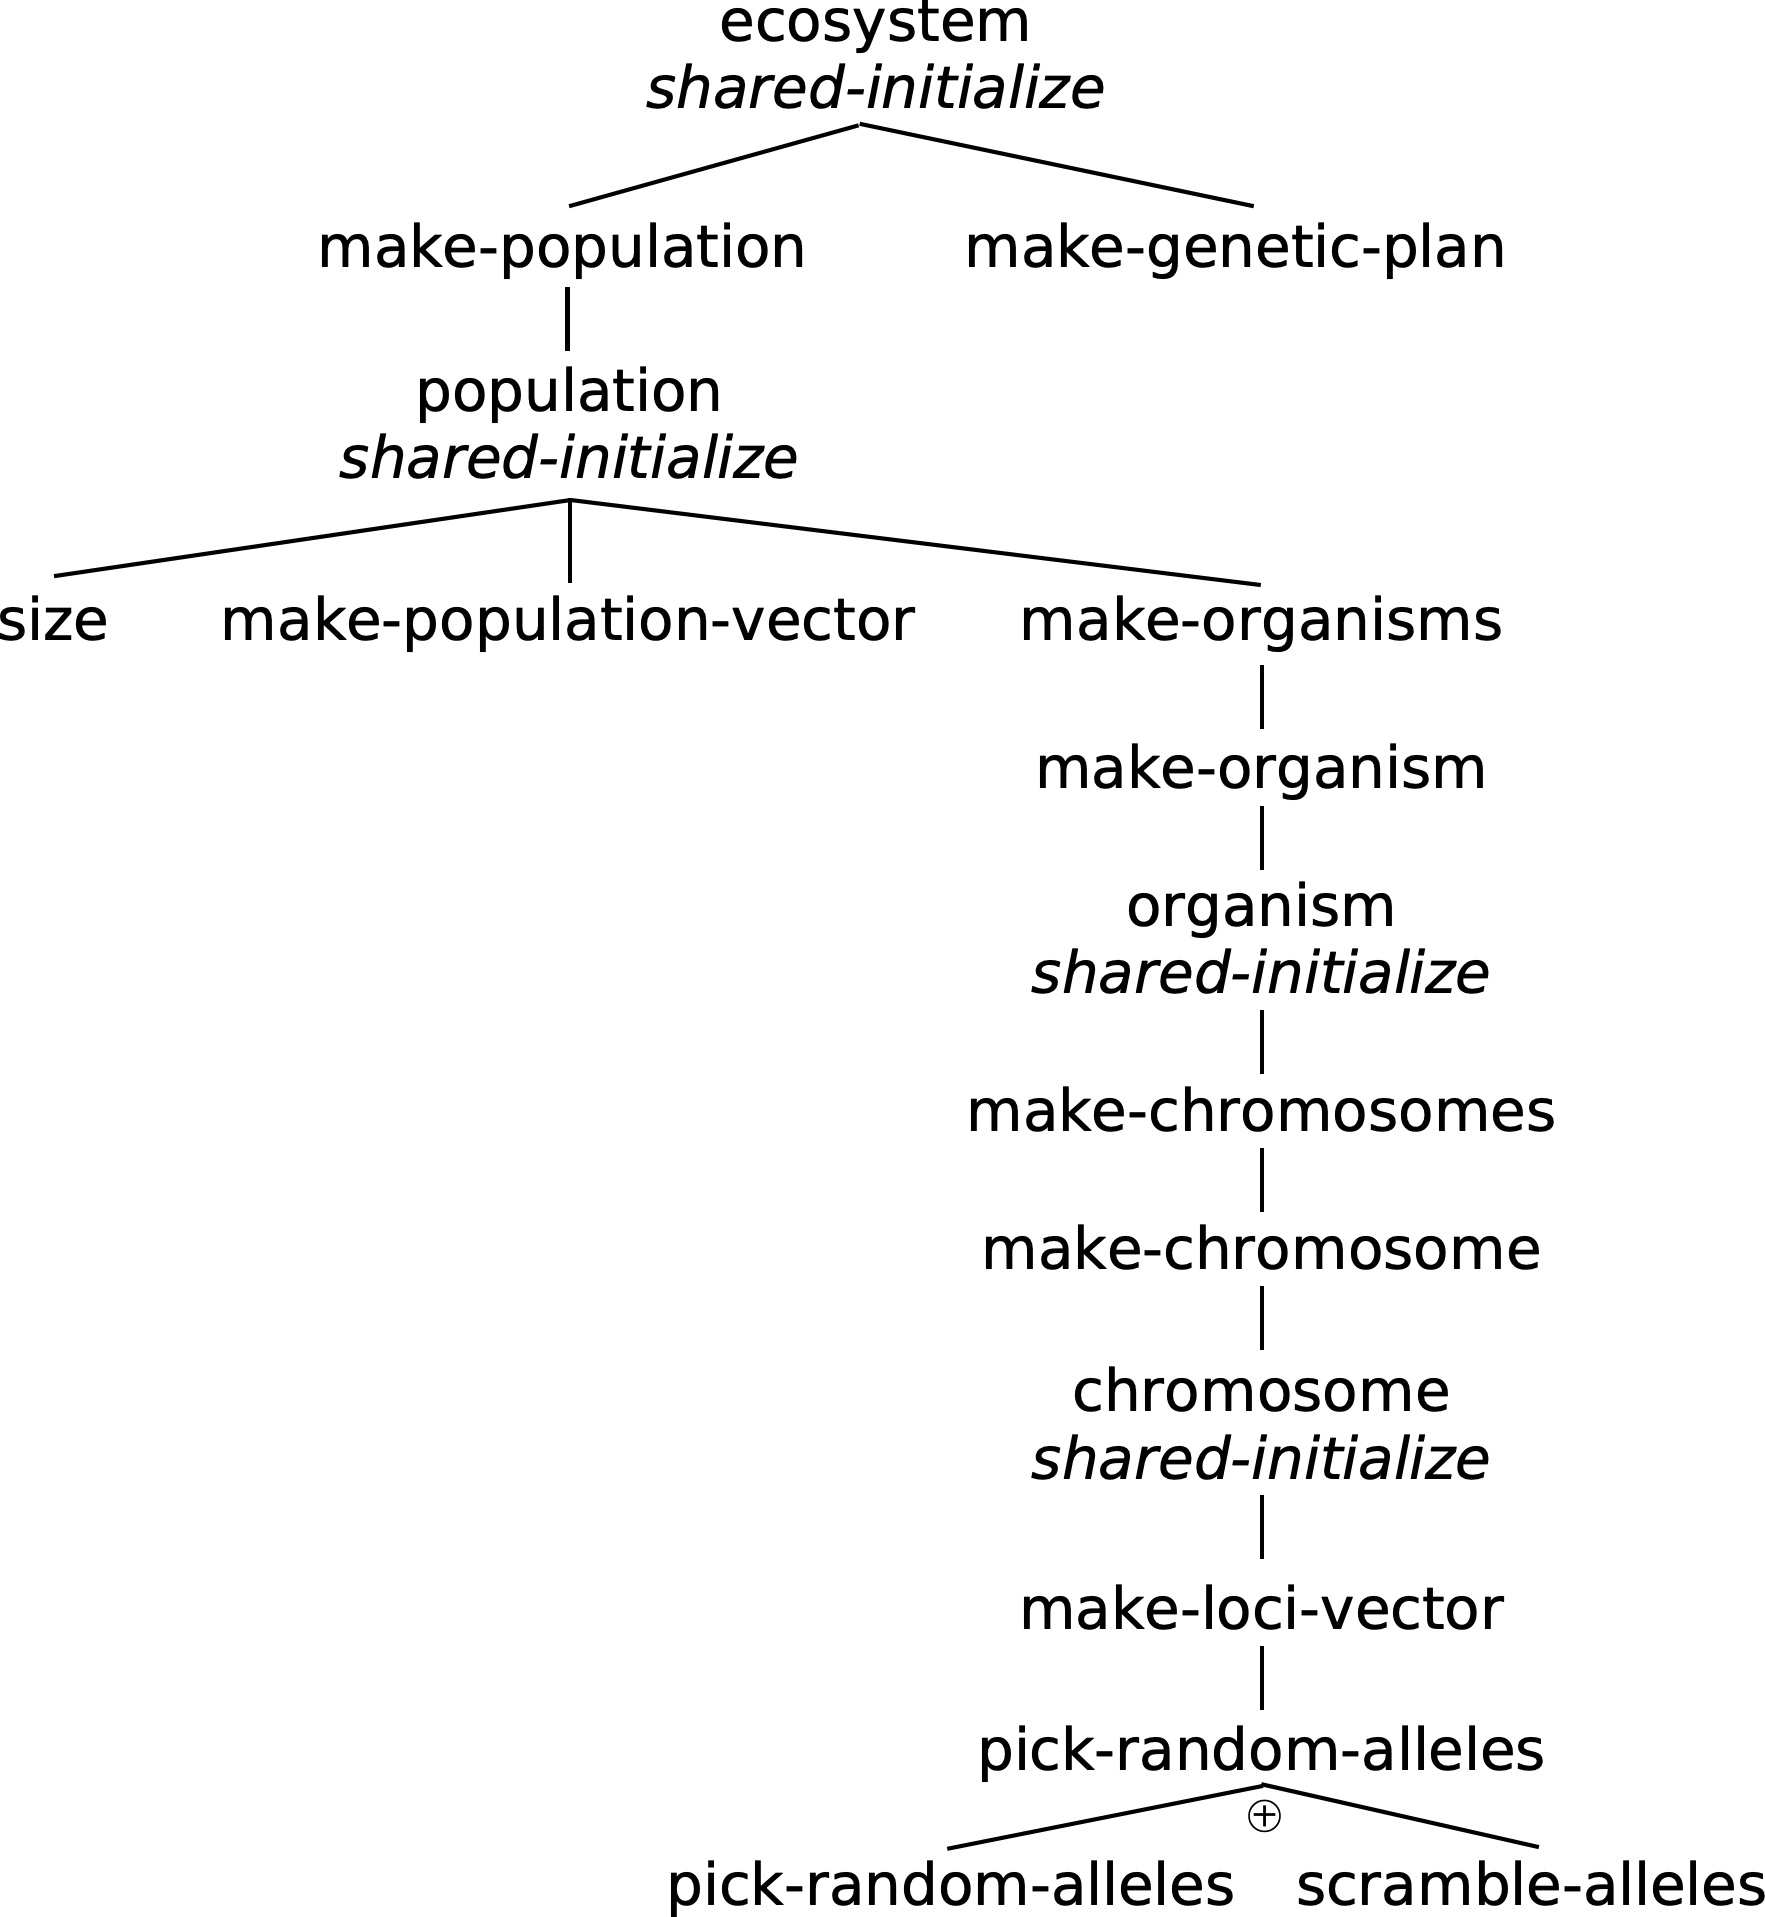
\includegraphics[width=\textwidth]{initialization-tree.eps}
  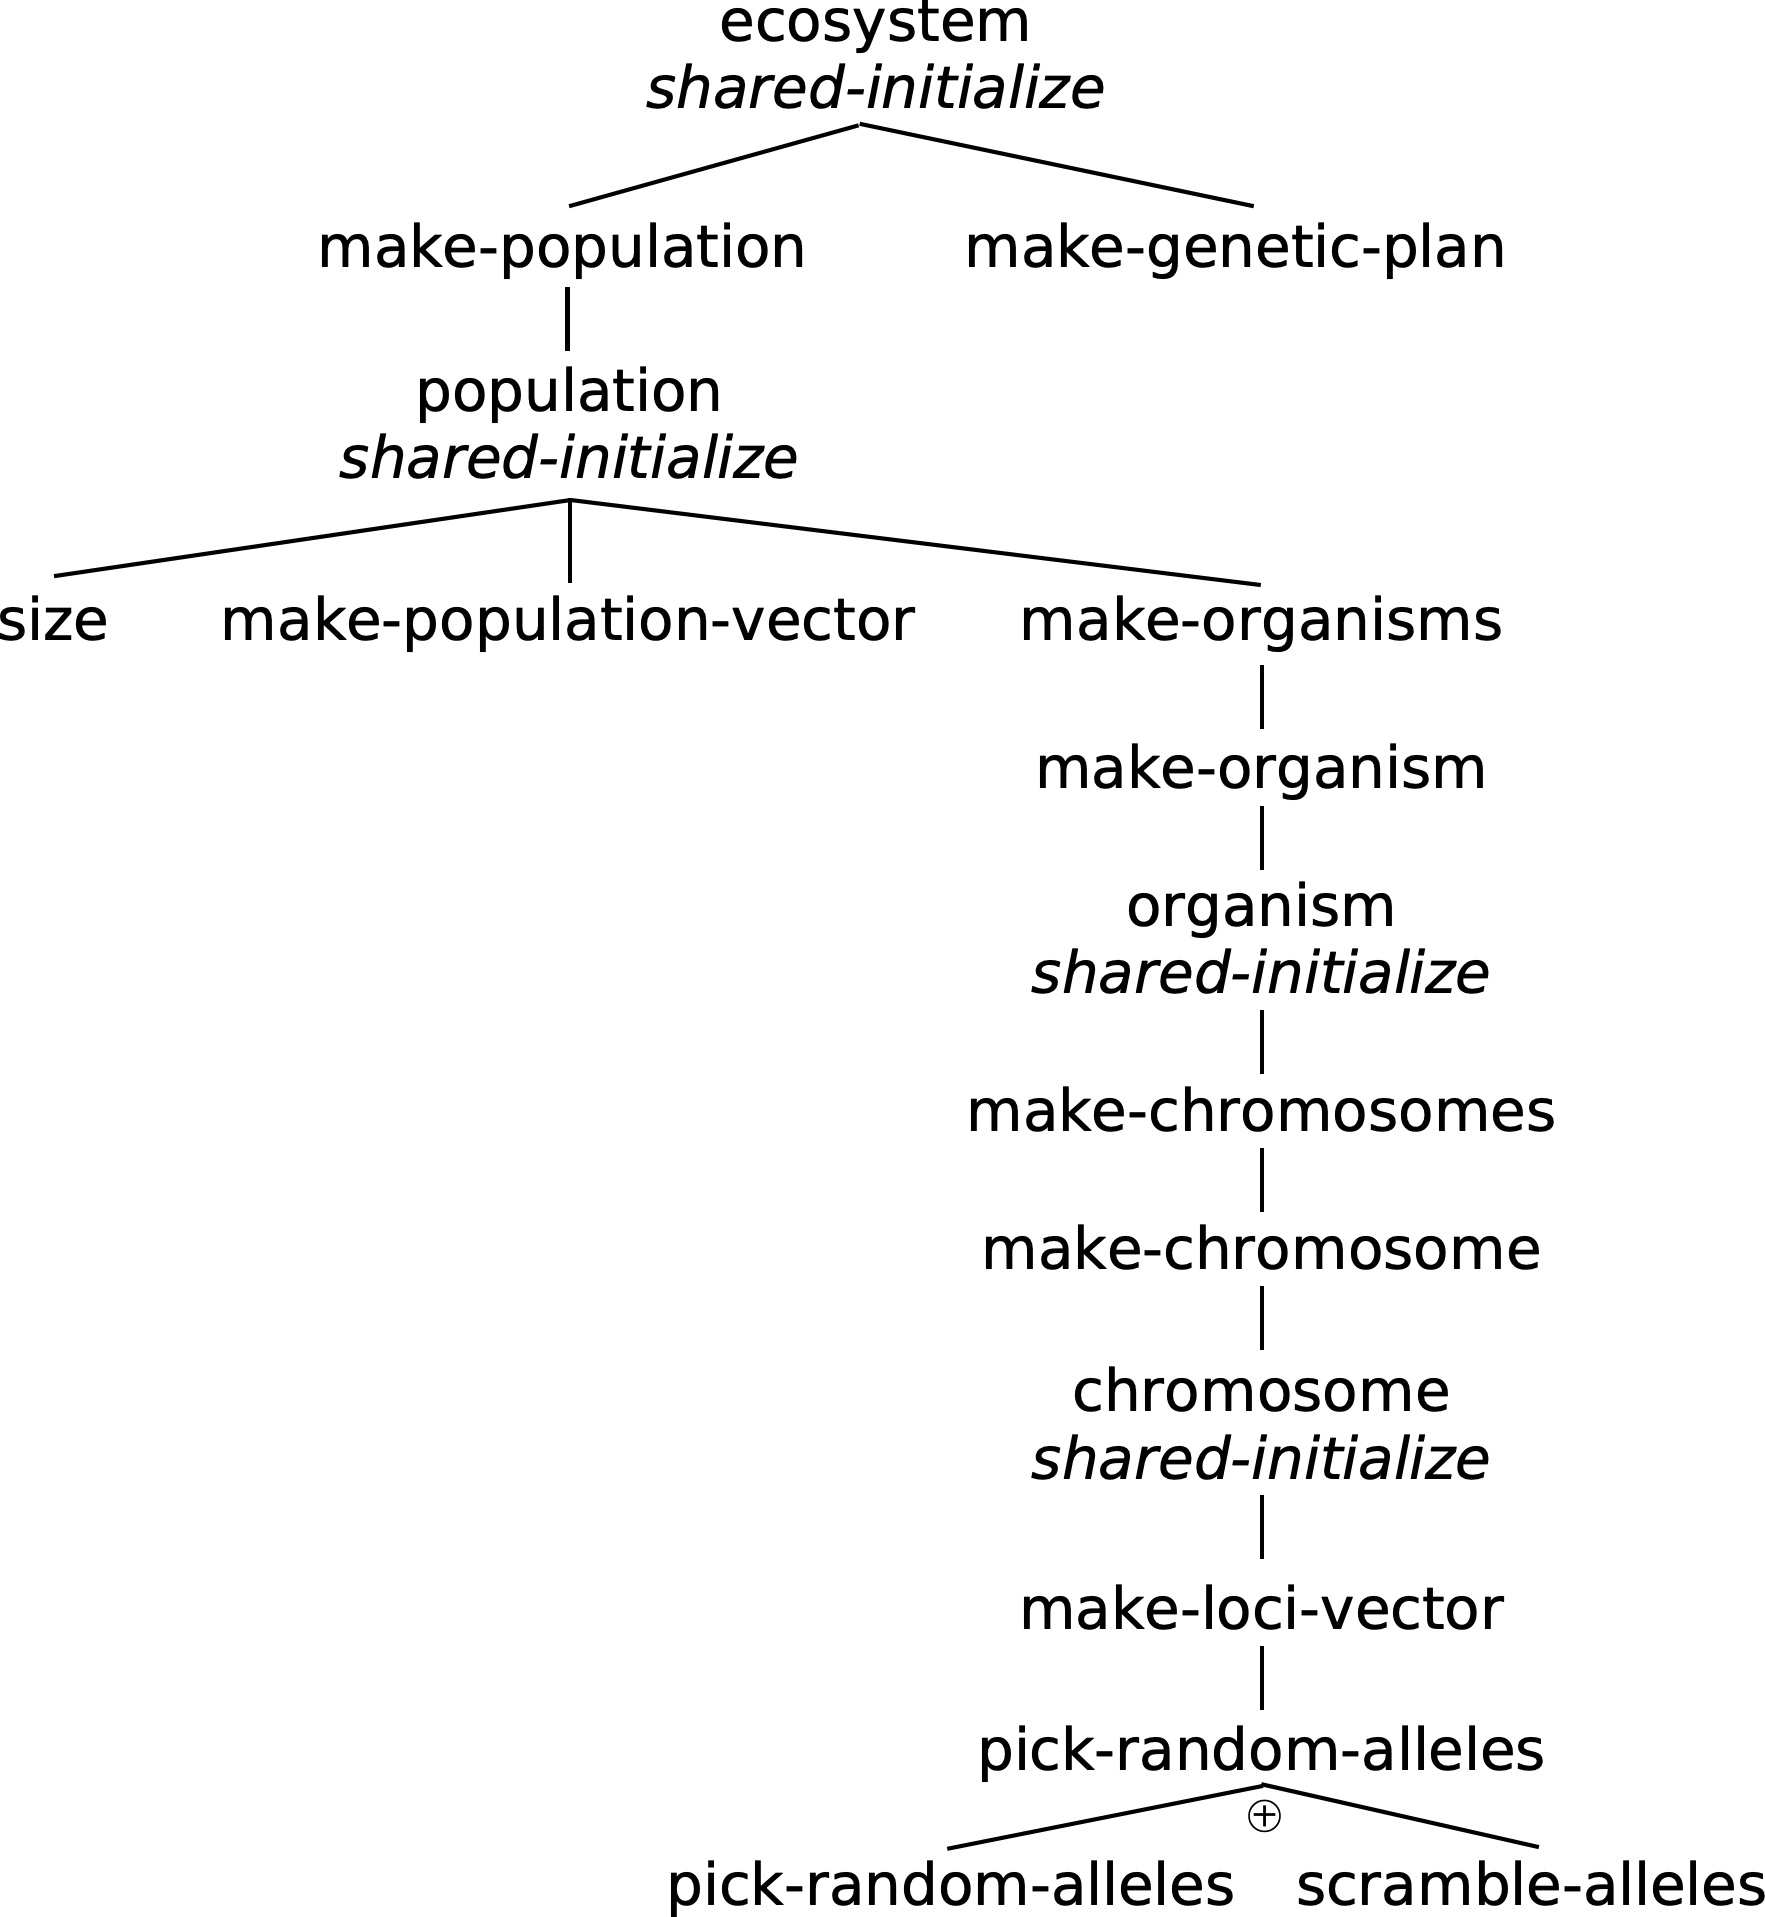
\includegraphics[width=0.6\textwidth]{initialization-tree.png}
  \caption{Call hierarchy for initialization of \Geco's principle structures}
  \label{fig:initialization-tree}
\end{figure}

\begin{figure}
  \centering
  % 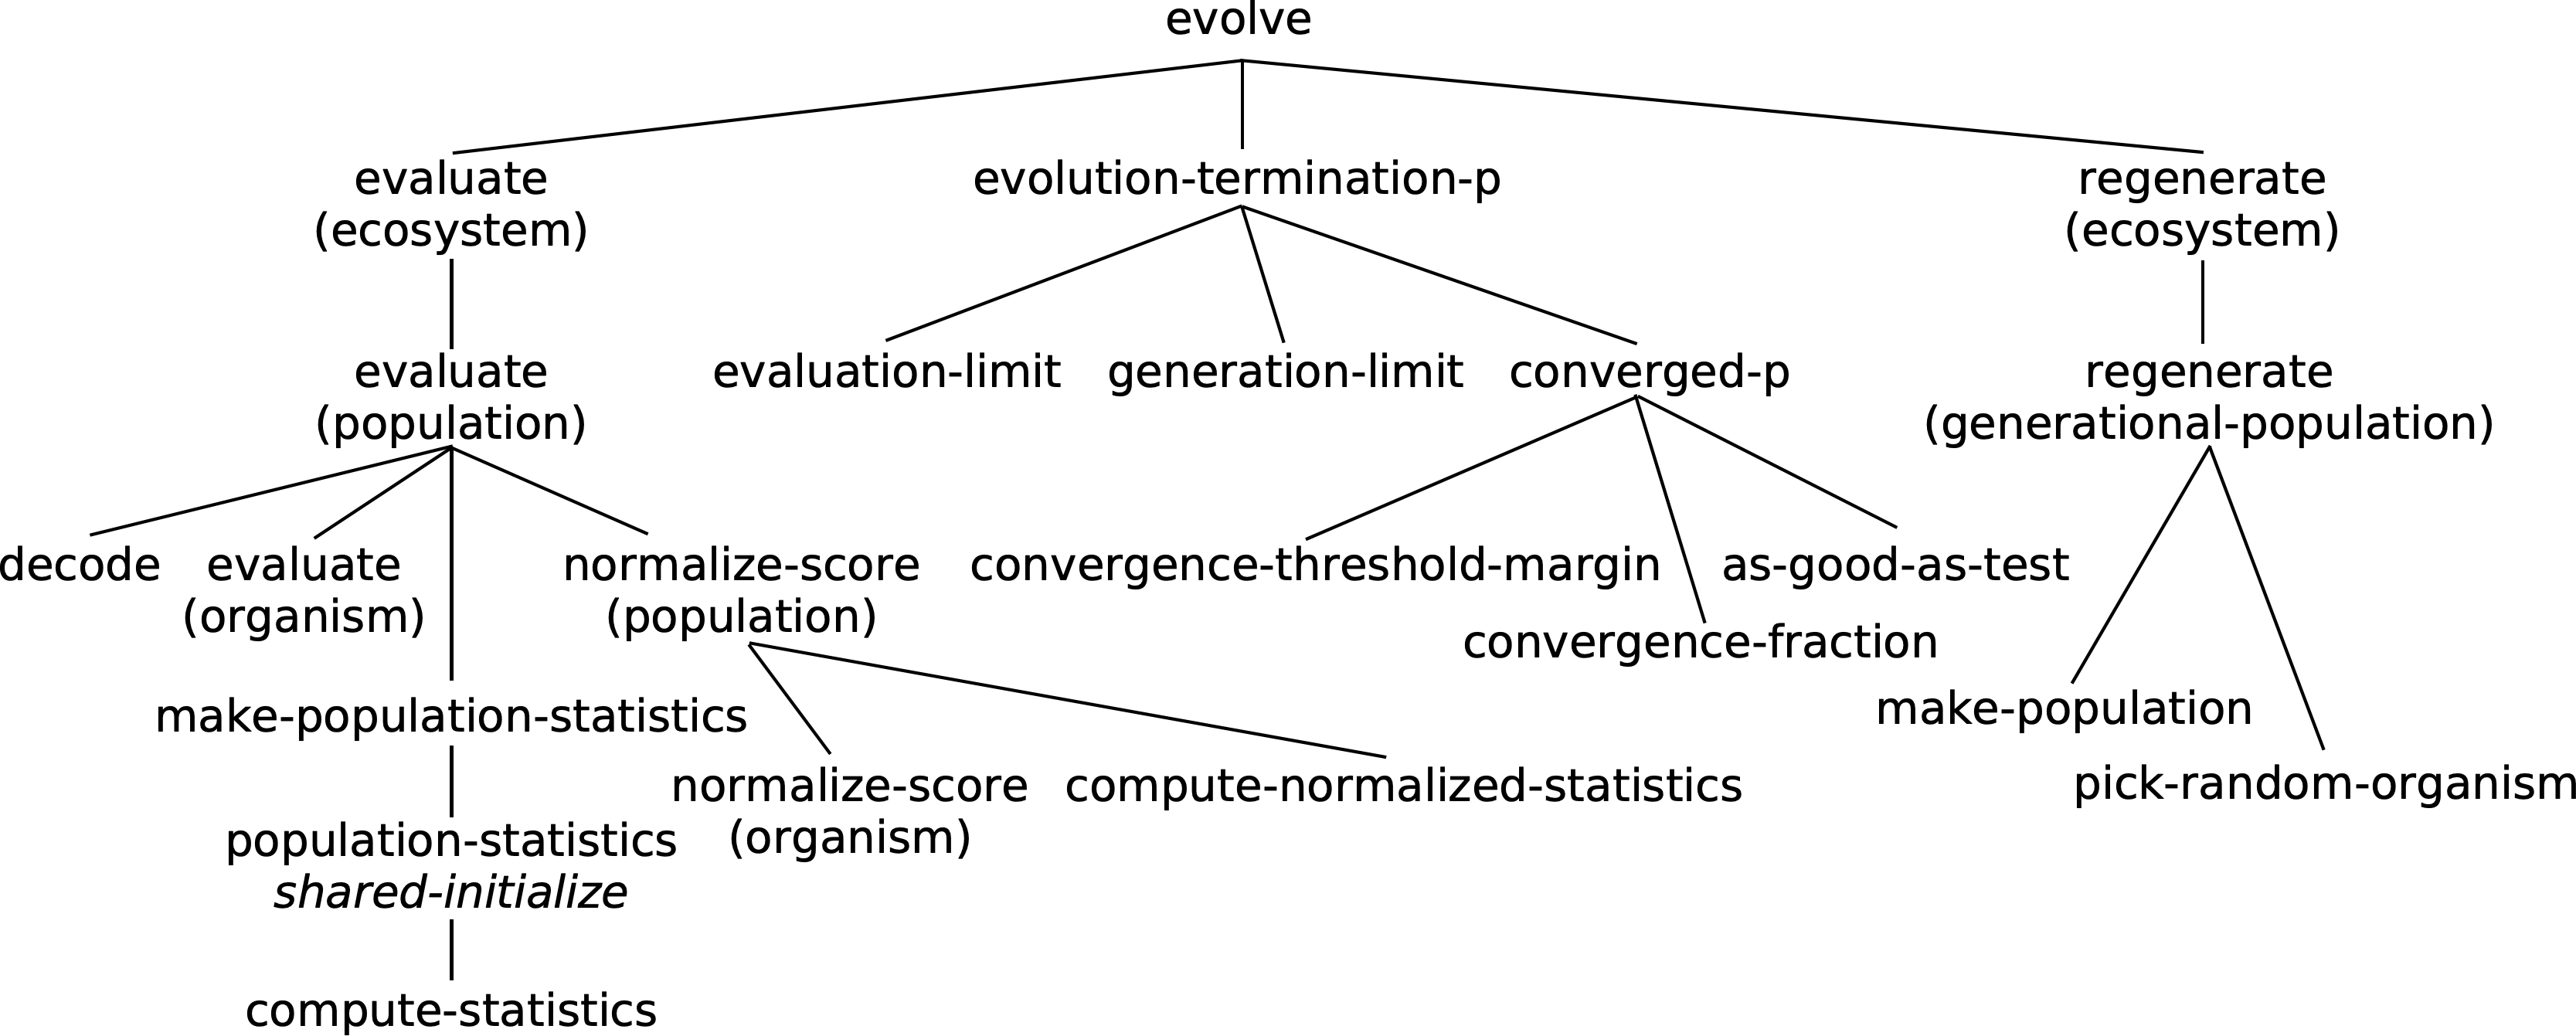
\includegraphics[width=\textwidth]{vert-evolve-tree.eps}
  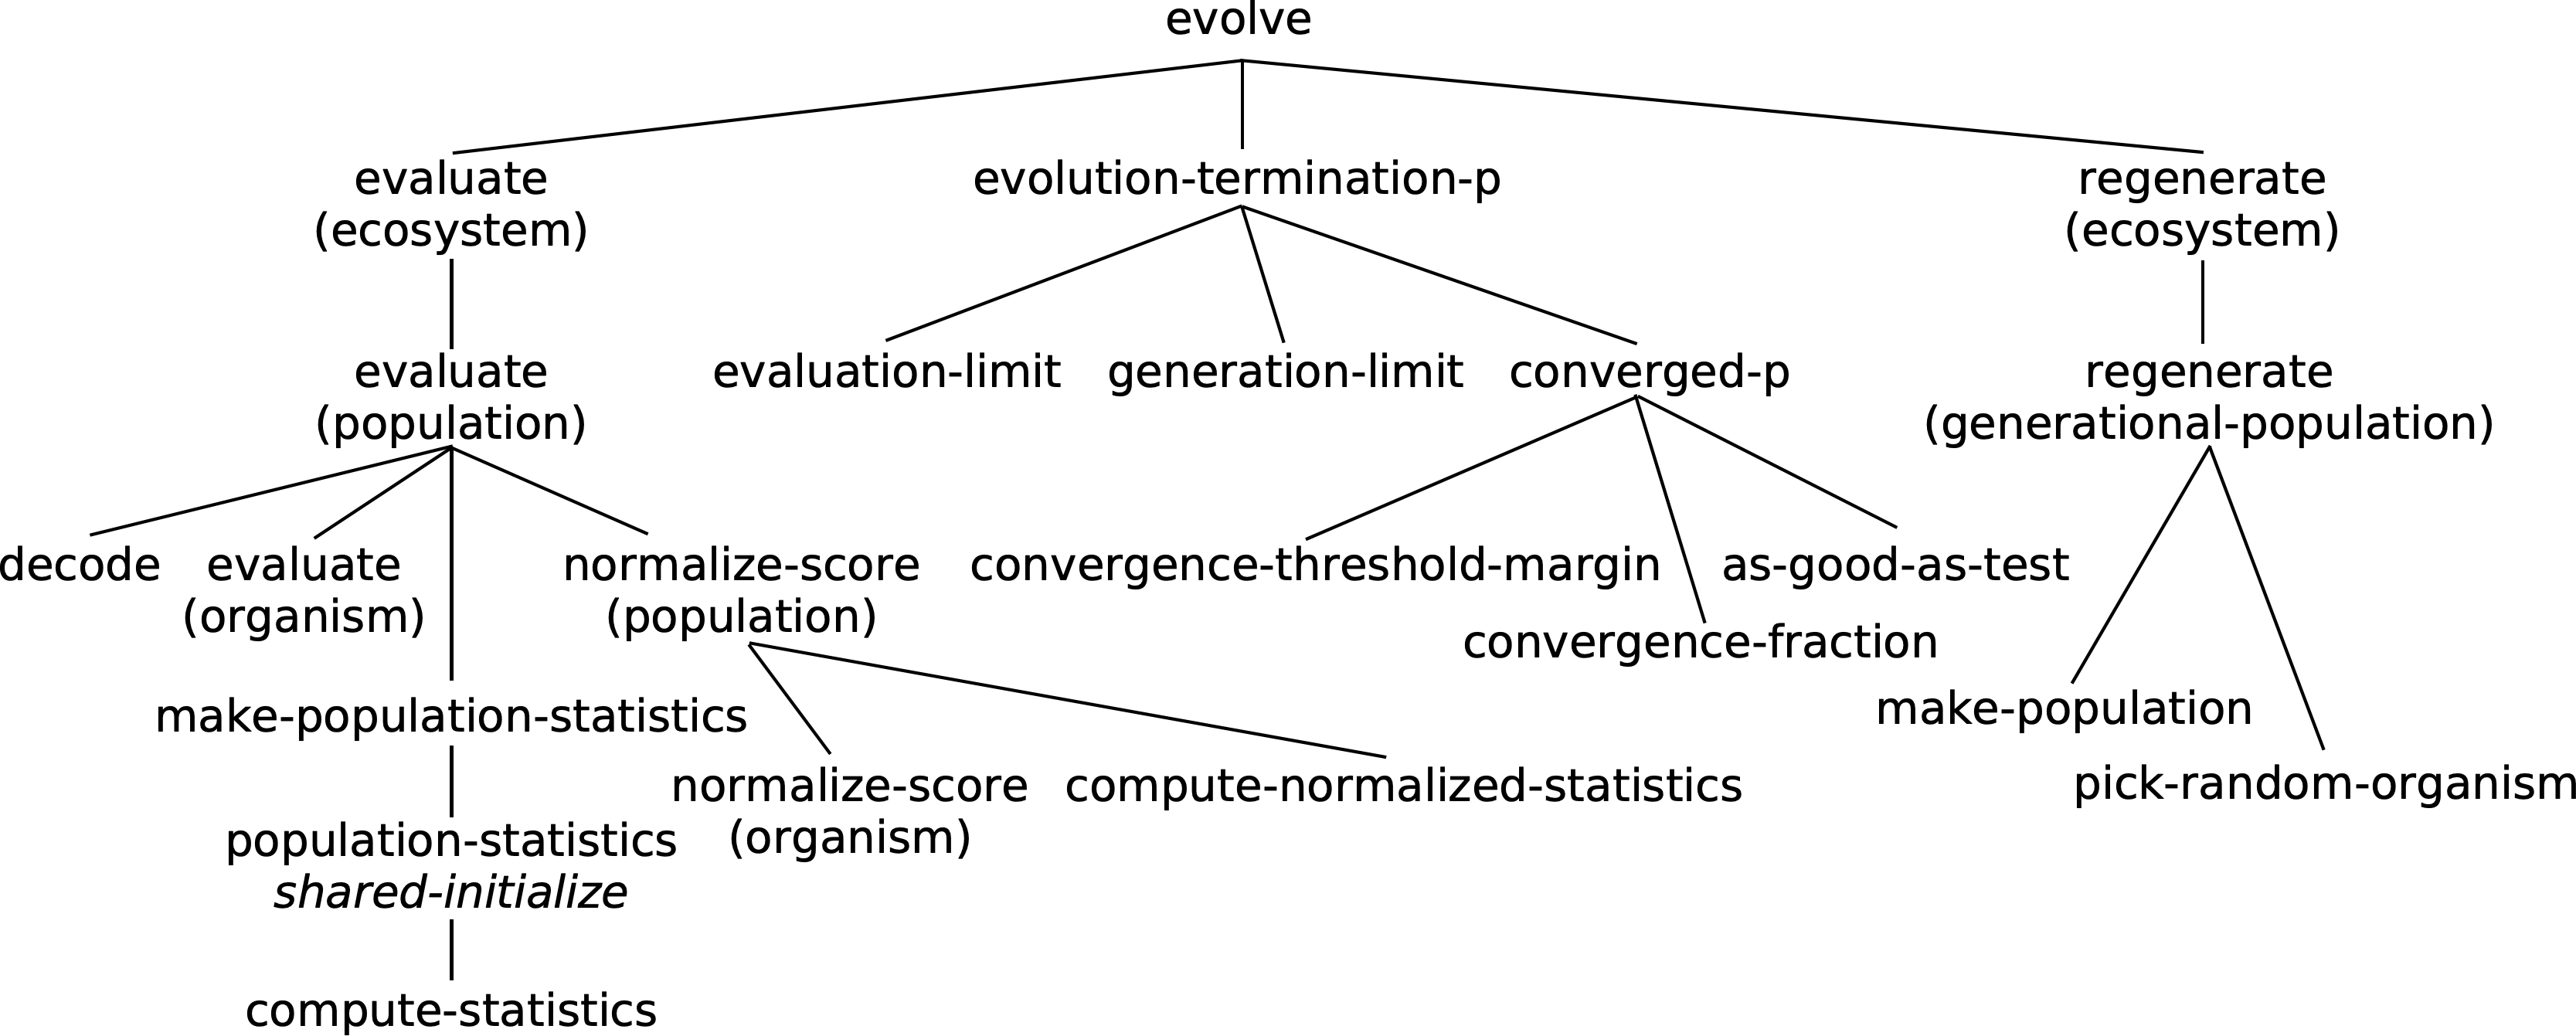
\includegraphics[width=\textwidth]{vert-evolve-tree.png}
  \caption{Call hierarchy for \Geco's evolutionary processing}
  \label{fig:evolve-tree}
\end{figure}

When supplied with the appropriate information, \geco\ can perform much of the
book-keeping, initialization, and control automatically.  This is made
possible by the built-in links between objects which are built upon the
\geco\ classes (see Figure~\ref{fig:class-interrelationships}).

\begin{figure}
  \centering	%% class-interrelationships.png is exported from class-interrelationships.pxd.pdf.cvd
  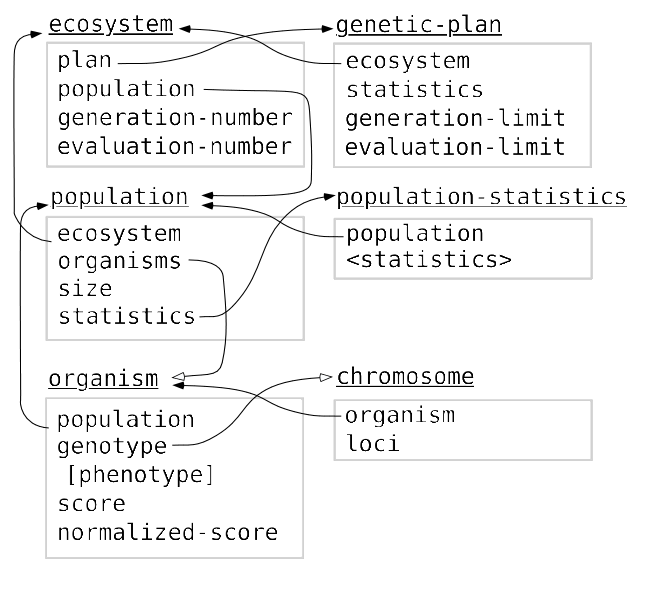
\includegraphics[width=0.75\textwidth]{class-interrelationships.png}
  % 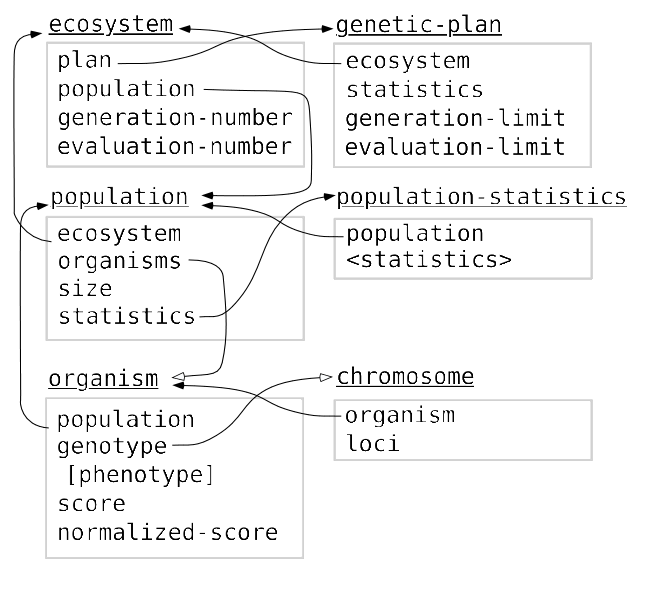
\includegraphics[]{class-interrelationships.png}
     \begin{center}
Solid head arrows indicate a one-to-one link;\\
hollow head arrows indicate a one-to-many link.
     \end{center}
  \caption{Interrelationships between \Geco\ objects}
  \label{fig:class-interrelationships}
\end{figure}



	% Copyright (C) 2020  George P. W. Williams, Jr.
\chapter{Details of GECO Classes and Functionality}

This chapter provides a more detailed discussion of each of \geco's 
classes, and the functionality implemented by their methods.   This functionality 
includes both the state retained by instances of each class (their {\em slots}),
and the functions (both generic and otherwise) which operate on those instances.

Even with all the functionality which \geco\ implements, it will still be
necessary to define some things which are specific to your application.
Generally this will be done by specializing \geco's classes (\ie, defining
some subclasses of \geco's builtin classes), and adding a few method
definitions to override and/or extend some of \geco's default behaviors.

Terminology Notes:

\begin{itemize}

\item In the material which follows, a statement which refers to `an instance of
\bold{a} {\it class-name} class' means that the instance is of the class
{\it class-name} or one of its subclasses. If the intent is to restrict the
instance to being of the named class, excluding subclasses, the wording will be
of the form `an instance of \bold{the} {\it class-name} class.'

\item In the descriptions of the methods, it will often be necessary to
distinguish between a generic function, a method for the generic function, and
the specific method supplied by \geco. A generic function and a method (as
specialized in the \term{flag line} above the description) are both parts of a
functional protocol which \geco\ expects to be honored.  A description
of a \geco-supplied method specifies that it
implements (fulfills) the requirements of this protocol.  \Geco\ may
define multiple methods (specialized for different classes) to implement
the generic function protocol for different classes.

\end{itemize}

For each class, the following sections will present the slots which 
are present in instances of the class (\ie, the values stored with each 
instance) and the functionality which has been defined for use with 
instances of the class (and its subclasses).
Generally, GAs implemented with \geco\ will not instantiate these classes.  
Instead, it will be more common to define subclasses which extend these 
classes (via added slots and methods) and specialize them (by overriding 
and/or extending inherited methods).


\section{The Ecosystem Class}

An \inxclass{ecosystem} is the highest level abstraction in a \geco\ implementation.
It is also the handle for manipulating a particular run of a GA. Since there may be
more than one instance of an \inxclass{ecosystem} in existence at one time, it is
possible to use \geco\ to create applications which use more than one GA at the same
time. The individual GAs could be competing, working on separate aspects of the same
problem, or they could be completely independent.
\filbreak
{\samepage

\Defclass {ecosystem}

\gap
\bold{Instance Allocated Slots}

  \Defslot {population}
  \defaccessor {population}

  An instance of a \inxclass{population} class.
  The population of an ecosystem is the set of organisms which are being 
  evolved.
\par}%end samepage

\filbreak

{\samepage
  \Defslotv {generation-number} {0}
  \defaccessor {generation-number}

  An integer, initially 0, which is 
  incremented each time the population enters a new {\em generation}.
  This happens each time the \inxgeneric{evolve}
  function is invoked on an \inxclass{ecosystem} instance (including
  \inxgeneric{evolve}'s recursive self-invocations). It should be noted
  that the actual creation of new members of the population (or creation
  of an entire new population) is expected to be handled by a \inxgeneric{regenerate}
  method specialized on a \inxclass{population} class, which
  is called by the default \geco-supplied \inxmethod{regenerate} method 
  specialized on \inxclass{ecosystem}.
\par}%end samepage

\filbreak

{\samepage
  \Defslotv {evaluation-number} {0}
  \defaccessor {evaluation-number}

  An integer, initially 0, which counts the number of times the 
  \inxgeneric{evaluate} function is applied to an \inxclass{organism} instance.
\par}%end samepage

\filbreak

{\samepage
  \Defslot {plan}
  \defaccessor {plan}

  An instance of a \inxclass{genetic-plan} class.
\par}%end samepage
\gap

\filbreak

The number of generations and evaluations are tracked by \geco\ so that the 
GA can be terminated based on the number of generations or evaluations 
exceeding some specific maximum limits, specified by the GA implementor.  
These limits are among the slots of the class \inxclass{genetic-plan}.

\filbreak
The \inxslot{population} and \inxslot{plan} are distinguished from the 
\inxclass{ecosystem} so that their classes may be specialized independently.  
Thus an instance of a single \inxclass{population} class may be manipulated 
using different \inxclass{plan}s, while instances of a single \inxclass{plan} may be 
used with different \inxclass{population}s.

\gap

\filbreak

{\samepage
	\bold{Instance Creation and Initialization}

The \inxclass{ecosystem} instance initialization has been extended by \geco\ by providing
a \cl{shared-initialize :AFTER} method for \inxclass{ecosystem}
to process the keyword arguments described below as follows:
\begin{itemize}
	\item If the call to \inxfun{make-instance}
	to create an instance of \inxclass{ecosystem} does not supply an initial population,
	then the \cl{:AFTER} method will initialize the \inxslot{population} slot using
	\inxgeneric{make-population}, with the values supplied via the \arg{:pop-class} and
	\arg{:pop-size} initargs.
	The call to \inxgeneric{make-population} also passes a value of \cl{t} for the \cl{:random}
	keyword argument, causing the initial population to be initialized to random organisms.
	(See Section~\ref{sec:population},
	page~\pageref{sec:population}.)
	
	\item Similarly, if a \inxclass{genetic-plan} instance is not supplied, then the \cl{:AFTER}
	method will initialize the \inxslot{plan} slot using \inxgeneric{make-genetic-plan}, with
	the value supplied via the \arg{:plan-class} initarg, and initializes the plan
	instance's \inxslot{generation-limit} and \inxslot{evaluation-limit} slots using the
	\arg{:gneration-limit} and \arg{:evaluation-limit} initargs. (See Section~\ref{sec:genetic-plan},
	page~\pageref{sec:genetic-plan}.)
\end{itemize}
The \inxgeneric{make-population} and \inxgeneric{make-genetic-plan} generic functions and
methods will be described subsequently, along with other \inxclass{ecosystem}-specialized
methods.
No special functions for the creation of \inxclass{ecosystem} instances have been defined,
since \inxgeneric{make-instance} and the standard \term{CLOS} protocol it follows provide all
the necessary functionality.

\par}%end samepage

\filbreak

{\samepage
\Definitarg {:plan-class}

  Provide the class for the \inxclass{genetic-plan} to be used by the
\inxclass{ecosystem}.
\par}%end samepage

\filbreak

{\samepage
\Definitarg {:pop-class}

  Provide the class for the \inxclass{population} instances to be created by
the \inxclass{ecosystem}.
\par}%end samepage

\filbreak

{\samepage
\Definitarg {:pop-size}

  Specifies the size to be used when the \inxclass{ecosystem} creates
\inxclass{population} instances.
\par}%end samepage

\filbreak

{\samepage
\Definitarg {:generation-limit}

This initarg is intended to specify the maximum number of generations which the ecosystem
will be allowed to evolve.
This limit is typically enforced by the \inxgeneric{evolution-termination-p} function
(see page~\pageref{evolution-termination-p}).
	
\par}%end samepage

\filbreak

{\samepage
\Definitarg {:evaluation-limit}

This initarg is intended to specify the maximum number of evaluations which the ecosystem
will be allowed to perform.
This limit is typically enforced by the \inxgeneric{evolution-termination-p} function
(see page~\pageref{evolution-termination-p}).

\par}%end samepage

\filbreak
\gap

{\samepage
\bold{Specialized Methods}

No special functions for the creation of \inxclass{ecosystem} instances have been defined
in \geco, since the \inxgeneric{make-instance} function and the standard \term{CLOS} protocol
it follows provide all the necessary functionality.
\par}% end \samepage

\filbreak

{\samepage

% use \Eggeneric so the CLOS generic isn't indexed
\Eggeneric shared-initialize {standard-object slot-names \rest initargs}
\defaftermethod shared-initialize {(ecosystem \inxclass{ecosystem}) slot-names \rest initargs
	\key :plan-class :pop-class :pop-size :generation-limit :evaluation-limit}

This method extends the initialization for \inxclass{ecosystem} instances to provide for the 
automatic creation and initialization of the \inxclass{population} and \inxclass{genetic-plan}
instances and slots.
The \inxgeneric{make-population} and \inxgeneric{make-genetic-plan} generic functions (described
next) are provided to support customization of these actions.
The call to \inxgeneric{make-population} in the default \geco-supplied method
passes a value of \cl{t} for the \cl{:random} keyword
argument, causing the initial population to be initialized to random organisms.
If \cl{:generation-limit} and \cl{evaluation-limit} are specified, the \inxslot{generation-limit}
and \inxslot{evaluation-limit} slots in the \inxclass{genetic-plan} instance are also initialized.
\par}% end \samepage

\filbreak

{\samepage

\Defgeneric make-population {ecosystem population-class \key :size :random}
\defmethod make-population {(ecosystem \inxclass{ecosystem}) population-class
	\key :size :random}
	\label{method:make-population}

This function provides an abstract interface to creation of a \inxclass{population} instance
to store in the \inxslot{population} slot of \arg{ecosystem}.
The primary \geco-supplied method
invokes \inxgeneric{make-instance} on the class \arg{population-class}, passing
the \arg{:size} argument, which determines the population size, and the
\arg{:random} argument, which if it is non-\cl{nil}, will cause the population to
be created with random organisms (intended for creation of the initial population).
It also returns the \inxclass{population} instance thus created.
\par}%end samepage

\filbreak

{\samepage
\Defgeneric make-genetic-plan {ecosystem genetic-plan-class}
\defmethod make-genetic-plan {(ecosystem \inxclass{ecosystem}) genetic-plan-class}
	\label{method:make-genetic-plan}

This function provides an abstract interface to creation of the \inxclass{genetic-plan}
instance for \arg{ecosystem}.  The \geco-supplied primary method invokes
\inxgeneric{make-instance} on \arg{genetic-plan-class}, and also supplies
\arg{ecosystem} so that the plan can be linked to the ecosystem (and vice-versa).
It also returns the \inxclass{genetic-plan} instance thus created.
\par}%end samepage

\filbreak

{\samepage
\Defgeneric evolve {ecosystem}
\defmethod evolve {(ecosystem \inxclass{ecosystem})}

This is the principle function which will be used by GA developers to invoke
their algorithm. The \geco-supplied primary method calls \inxmethod{evaluate} on
\arg{ecosystem}, and if the termination\index{termination} condition has not been
reached (see \inxgeneric{evolution-termination-p}), creates a new generation of
its \inxslot{population} via the \inxgeneric{regenerate} function, and
recurses to evolve some more\footnote{See the discussion in the footnote on
page~\pageref{recursive-vs-iterative-evolve}}.
The value returned by this function is not defined.
\par}%end samepage

\filbreak

{\samepage  
\Defgeneric evaluate {thing genetic-plan}
\defmethod evaluate {(ecosystem \cl{ecosystem}) genetic-plan}

The purpose of this function is to cause \arg{thing} to be evaluated according to
the specified \term{genetic plan}. The \geco-supplied primary method for
\inxclass{ecosystem} instances evaluates \arg{ecosystem} by calling
\inxgeneric{evaluate} on its \inxslot{population} with \arg{genetic-plan}. (Also
see the \inxmethod{evaluate} method specialized for the class \inxclass{population}, on
page~\pageref{evaluate-population}.)
The value returned by this function is not defined.
\par}%end samepage

\filbreak


\section{The Population Class} \label{sec:population}

A population is the most global structure upon which a GA operates. Although
\term{genetic operator}s are applied to the members (\term{organism}s in 
\geco's terminology, though they are often called
\ital{individuals}) of a population, it is at the level of the population that
the GA is really working.

\filbreak

{\samepage
\Defclass {population}

Instances of \inxclass{population} classes collect all the \inxclass{organism} 
instances of a generation.
\par}%end samepage

\gap

\filbreak

{\samepage
\bold{Instance Allocated Slots}

\Defslot {ecosystem}
\definitarg {:ecosystem}
\defaccessor {ecosystem}

Provides a link back to the \inxclass{ecosystem} instance to which the population belongs.
\par}%end samepage

\filbreak

{\samepage
\Defslot {organisms}
\defaccessor {organisms}

A vector, which contains all the \inxclass{organism} instances in the population.
\par}%end samepage

\filbreak

{\samepage
\Defslotv {size} {nil}
\definitarg {:size}
\defaccessor {size}

Either \cl{nil} or an integer, which indicates the size of the population, \ie,
the size of the vector in the \inxslot{organisms} slot. When \cl{nil}, the
organism vector will not be created automatically. \par}%end samepage

\filbreak

{\samepage
\Defslot {statistics}
\definitarg {:statistics}
\defaccessor {statistics}

An instance of a \inxclass{population-statistics} class, which holds statistics
\geco\ needs for the population. The \inxclass{population-statistics} class is
distinct from the \inxclass{population}class so that their sub-classes and methods may 
be specialized independently. 
\par}%end samepage

\gap
\filbreak

{\samepage

\bold{Instance Creation and Initialization}

The generic function \inxgeneric{make-population} (see page~\pageref{method:make-population})
is the \geco\ interface for creation of \inxclass{population} instances.

The initialization for instances of \inxclass{population} has been extended to
provide for automatic creation and initialization of the \inxslot{organisms}
vector. The functions \inxgeneric{make-organisms-vector} and
\inxgeneric{make-organisms} are used to permit customization of these
initialization actions; \inxgeneric{make-organisms-vector} is called when the
\inxslot{size} slot has a non-\cl{nil} value, and \inxgeneric{make-organisms} is
called only when both \inxslot{size} and \inxinitarg{:random} (below) have
non-\cl{nil} values. It is the responsibility of the \term{genetic plan} to
create the organisms after the initial generation.
\par}%end samepage

\filbreak

{\samepage
The \inxclass{population} instance initialization has been extended to support the following
additional initarg:

\Definitarg {:random}

The value of this keyword is passed to \inxgeneric{make-organisms}, and is intended
to support automatic initialization of the initial population to random organisms.
\par}%end samepage
\gap
  
\filbreak

{\samepage

\bold{Specialized Methods}

Note that most (if not all) of the generic functions in
Section~\ref{sec:selection-methods}, Selection Methods, have methods which
are specialized on the \inxclass{population} class.

\filbreak

{\samepage
	
% use \Eggeneric so the CLOS generic isn't indexed
\Eggeneric shared-initialize {standard-object slot-names \rest initargs}
\defaftermethod shared-initialize {(pop \inxclass{population}) slot-names \rest initargs
	\key :random}

This method extends the initialization for \inxclass{population} instances to provide for the 
automatic creation and initialization of the \inxclass{organism} instances for the population.
In the \geco-supplied default method, if the \inxslot{organisms} slot of 
\arg{pop} is unbound, the \inxgeneric{make-organisms-vector} generic function
(see below) is invoked to initialize the \inxslot{organisms}
slot; and then, if the \arg{:random} keyword argument is non-\cl{nil}, the
\inxgeneric{make-organisms} function (see below) is invoked to initialize
the population's organism vector to random organisms.
\par}% end \samepage

\filbreak

{\samepage
\Defgeneric make-organisms-vector {population size}
\defmethod make-organisms-vector {(population \inxclass{population}) size}

This function provides an abstract interface to creation of the population's
organisms vector (the vector which holds \arg{population}'s organisms). The
\arg{size} argument determines the size of the vector. The \geco-supplied primary
method uses the Common Lisp function \cl{make-array} to create an array of the
specified size.
It also returns the the array thus created.
\par}%end samepage

\filbreak

{\samepage
\Defgeneric make-organisms {population \key :random}
\defmethod make-organisms {(population \inxclass{population}) \key :random}

This function provides an abstract interface to creation of the organisms in
\arg{population}'s organisms vector. The \arg{:random} argument, when
non-\cl{nil}, causes all the new organisms to be random (\ie, have randomly
chosen chromosomes). The \geco-supplied primary method invokes
\inxgeneric{make-organism} for each position in the organisms vector. The
\arg{:random} argument is passed to each call to \inxgeneric{make-organism}.
The value returned by this function is not defined.
\par}%end samepage

\filbreak

{\samepage
\Defgeneric make-organism {population \key :random :no-chromosome}
\defmethod make-organism {(population \inxclass{population}) \key :random :no-chromosome}
	\label{method:make-organism}

This function provides an abstract interface to creation of a single organism
based on the \inxgeneric{organism-class} of \arg{population}. The \arg{:random}
argument, when non-\cl{nil}, causes the new organism to be random (\ie, have
randomly chosen chromosomes). The \arg{:no-chromosome} argument, when
non-\cl{nil}, causes the organism to be created without chromosomes, avoiding
wasted work when the chromosomes will be supplied by other mechanisms, \eg,
\term{genetic operator}s. The \geco-supplied primary method passes \arg{population} to
the call to \inxgeneric{make-instance} so that the organism can have a back-link
to the population to which it belongs. The \arg{:random} and
\arg{:no-chromosomes} arguments are passed to \inxgeneric{make-instance}.
It also returns the the \inxclass{organism} instance thus created.
\par}%end samepage

\filbreak

{\samepage
\Defgeneric organism-class {population}

This function returns the class to be used to create organisms which will become members
of \arg{population}. The GA developer {\em must implement the primary method} for all
subclasses of the class \inxclass{population}. \Geco\ does not provide a default primary method
specialized on the \inxclass{population} class.\footnote{There are comments at the beginning
of the {\tt generics.lisp} file which summarize the functions which should or must be
defined to implement a working GA using \geco.}
\par}%end samepage

\filbreak

{\samepage
\Defgeneric evaluate {thing genetic-plan}
\defmethod evaluate {(population \inxclass{population}) (genetic-plan \inxclass{genetic-plan})}
\label{evaluate-population}

This function evaluates \arg{thing} according to \arg{genetic-plan}. This method
assures that each organism in \arg{population} is evaluated. The \geco-supplied
primary method only calls \inxgeneric{evaluate} on an organism if the organism
doesn't already have a \term{score} in its \inxslot{score} slot. After
\arg{population} has been evaluated, \inxgeneric{normalize-score} and
\inxgeneric{make-population-statistics} are called to assure that normalized
scores and statistics have been computed for the population.
The value returned by this function is not defined.
\par}%end samepage

\filbreak

{\samepage
\Defgeneric make-population-statistics {population}
\defmethod make-population-statistics {(population \inxclass{population})}
	\label{method:make-population-statistics}

This function provides an abstract interface to creation of the
\inxclass{population-statistics} instance for \arg{population}, based on the
\inxgeneric{population-statistics-class} of \arg{population}. The \geco-supplied
primary method passes \arg{population} to \inxgeneric{make-instance} so that the instance can
have a back-link to the population to which it belongs.
It also returns the \inxclass{population-statistics} instance thus created.
\par}%end samepage

\filbreak

{\samepage
\Defgeneric compute-statistics {population}
\defmethod compute-statistics {(population \inxclass{population})}

This function provides an abstract interface for computing statistics for
\arg{population}. This method provieds a place for a population class to provide
for customization of statistics computation. The \geco-supplied primary method
simply calls \inxgeneric{compute-statistics} on the statistics instance of
\arg{population}. (Also see the description of \inxmethod{compute-statistics}
on page~\pageref{compute-population-statistics},
specialized on the class \inxclass{population-statistics}, and
Section~\ref{sec:pop-stats-class}, which details the statistics that are computed.)
The value returned by this function is not defined.
\par}%end samepage

\filbreak

{\samepage
\Defgeneric compute-binary-allele-statistics {population}
\defmethod compute-binary-allele-statistics {(population \inxclass{population})}

This function returns a list of vectors (one per binary chromosome in the
organisms of \arg{population}) of counts (\cl{fixnum}s), by locus, of non-zero
alleles. For example, if the organisms in a population contain $c$ binary
chromosome (and any number of non-binary chromosomes), and each binary chromosome
contains $b$ loci, then this function will return a list containing $c$ vectors
of $b$ fixnums. Each \cl{fixnum} in the returned vectors is a count of non-zero
alleles in the entire population at the locus whose index corresponds to the
index into the $c^{\rm th}$ vector of counts. \Eg, if the third count in the
first vector is 7, then the entire population contains 7 non-zero alleles in
locus 3 of the first binary chromosome of each organism.
\par}%end samepage

\filbreak

{\samepage
\Defgeneric normalize-score {thing plan}
\defmethod normalize-score {(population \inxclass{population})
                            \hbox{(genetic-plan \inxclass{genetic-plan})}}

This function computes the normalized
\term{score}(s)\index{score!normalization}\index{normalization} for \arg{thing}.
This method computes the normalized scores for all organisms in \arg{population}.
The \geco-supplied primary method for \inxclass{population} invokes
\inxgeneric{normalize-score} (see page \pageref{method:normalize-score:organism})
for each organism in \arg{population}, according to the \arg{genetic-plan}, and
updates \cl{(statistics \arg{population})} with normalized values using the function
\inxgeneric{compute-normalized-statistics}.
The value returned by this function is not defined.

[Note that \geco\ version 2.1 changed the calling sequence for this generic function and all its methods.]
\par}%end samepage

\filbreak

There are a number of different ways to normalize\index{normalization} the
scores. With some plans and evaluation functions, it may not even be necessary,
though beware that the score should always be $\ge 0$ (see Chapter 4 of
\cite{ga:goldberg}, under the sections on Scaling Mechanisms and Ranking
Procedures).

\filbreak

{\samepage
\Defgeneric population-statistics-class {population}
\defmethod population-statistics-class {(population \inxclass{population})}

This function returns the population-statistics class which will be used for
\arg{population.} The \geco-supplied primary method specialized for the
\inxclass{population} class returns \inxclass{population-statistics}.
\par}%end samepage

% This function could be performed by \cl{:allocation :per-class} slots 
% if and when they can be implemented portably in Common Lisp.

\filbreak

{\samepage
\Defgeneric converged-p {population}
\defmethod converged-p {(population \inxclass{population})}
	\label{population:converged-p}
This function is a predicate which indicates whether \arg{population} has
\concept{converged}, which is useful as a termination\index{termination}
condition. The \geco-supplied primary method defines convergence as
either of the following:
\par}%end samepage

\filbreak

{\samepage
  \begin{enumerate}
    \item All organisms in \arg{population} have the same \inxslot{score}; or
    \item At least a portion of \arg{population} (specified by the
        \inxgeneric{convergence-fraction} function) has a 
        \inxslot{normalized-score} which is {\em as good as} the value specified by the
        \inxgeneric{convergence-threshold-margin} function.
  \end{enumerate}
}%end samepage

\filbreak

Note that this allows \geco\ to either {\em maximize} or {\em minimize}
\term{scores}. The mechanism for determining whether \geco\ maximizes or minimizes,
and hence how it determines {\em as good as} or {\em better than}, is determined by
mixing one of two classes with the population class used by the GA. These
\term{mixin classes} are described below, in section
\ref{sec:population-mixin-classes}.

\filbreak

{\samepage
\subsection{Subclasses of Population}

\Defclassv {generational-population} {population}

This class is a subclass of \inxclass{population} which provides explicit support
for the `standard' generational style of GA. The class has no
slots, but methods described elsewhere specialize on this class (see
\inxmethod{regenerate}, page~\pageref{method:regenerate}).
\par}%end samepage
\filbreak

Eventually \geco\ may contain support for other styles of population handling,
possibly including parallel sub-populations, steady-state populations, \etc.

\gap
\filbreak

{\samepage
\bold{Instance Creation and Initialization}

The generic function \inxgeneric{make-population} (see
page~\pageref{method:make-population}) is the \geco\ interface for creation
of instances of \inxclass{population} and its subclasses.
\par}%end samepage

\filbreak

{\samepage
\subsection{Population Mixin Classes}	\label{sec:population-mixin-classes}

\Defclass {maximizing-score-mixin}
\defclass {minimizing-score-mixin}

Neither of these classes has any slots or has special provisions for
instance creation or initialization.
\par}%end samepage

\gap

\filbreak

{\samepage

\bold{Specialized Methods}

Both classes implement methods for the following generic functions:

\Defgeneric maximizing-p {population}
\defmethod maximizing-p {(population \inxclass{maximizing-score-mixin})}
\defmethod maximizing-p {(population \inxclass{minimizing-score-mixin})}
\Defgeneric minimizing-p {population}
\defmethod minimizing-p {(population \inxclass{maximizing-score-mixin})}
\defmethod minimizing-p {(population \inxclass{minimizing-score-mixin})}

These functions permit algorithms to efficiently determine whether the
\arg{population} is minimizing or maximizing.  The \geco-supplied methods
return either \cl{t} or \cl{nil} as appropriate for their class.
\par}%end samepage

%These functions could all be performed by \cl{:allocation :per-class} slots if
%and when they can be implemented portably in Common Lisp.

\filbreak

{\samepage
\Defgeneric convergence-fraction {population}
\defmethod convergence-fraction {(population \inxclass{maximizing-score-mixin})}
\defmethod convergence-fraction {(population \inxclass{minimizing-score-mixin})}

This function returns the convergence-fraction value which should be used for
\arg{population} by the \inxgeneric{converged-p} function. The \geco-supplied
primary methods for both the \inxclass{maximizing-score-mixin} and the
\inxclass{minimizing-score-mixin} classes return $0.95$. These values are not
necessarily the {\em right} numbers in any real sense, but they are probably
reasonable for many applications. Some applications may want to provide different
values, and possibly even adaptive methods for specialized subclasses.
\par}%end samepage

\filbreak

{\samepage
\Defgeneric convergence-threshold-margin {population}
\defmethod convergence-threshold-margin {(population \inxclass{maximizing-score-mixin})}
\defmethod convergence-threshold-margin {(population \inxclass{minimizing-score-mixin})}

This function returns the convergence-threshold-margin value which should be used
for \arg{population} by the \inxgeneric{converged-p} function. The \geco-supplied
primary method provided for the \inxclass{maximizing-score-mixin} class returns
$0.95$, and the method provided for the \inxclass{minimizing-score-mixin} class
returns $0.05$. These values are not necessarily the {\em right} numbers in any real
sense, but they are probably reasonable for many applications. Some applications may
want to provide different values, and possibly even adaptive methods for specialized
subclasses. 
\par}%end samepage

\filbreak

{\samepage
\Defgeneric as-good-as-test {population}
\defmethod as-good-as-test {(population \inxclass{maximizing-score-mixin})}
\defmethod as-good-as-test {(population \inxclass{minimizing-score-mixin})}

This function returns a function of two numeric arguments, which when applied to
\inxslot{score}s from organisms in \arg{population}, indicates whether or not the first
score is as good as the second. The \geco-supplied primary method for the
\inxclass{maximizing-score-mixin} class returns \cl{#'>=}, and the method provided
for the \inxclass{minimizing-score-mixin} class returns \cl{#'<=}.
\par}%end samepage

\filbreak

{\samepage
\Defgeneric better-than-test {population}
\defmethod better-than-test {(population \inxclass{maximizing-score-mixin})}
\defmethod better-than-test {(population \inxclass{minimizing-score-mixin})}

This function returns a function of two numeric arguments, which when applied to
\inxslot{scores} from organisms in \arg{population}, indicates whether or not the first
score is better than the second. The \geco-supplied primary method provided
for the \inxclass{maximizing-score-mixin} class returns \cl{#'>}, and the method
provided for the \inxclass{minimizing-score-mixin} class returns \cl{#'<}.
\par}%end samepage

\filbreak

{\samepage
\Defgeneric best-organism {population}
\defmethod best-organism {(population \inxclass{maximizing-score-mixin})}
\defmethod best-organism {(population \inxclass{minimizing-score-mixin})}

This function returns the best organism in the corresponding population from
population statistics of \arg{population}. The \geco-supplied primary method for the
\inxclass{maximizing-score-mixin} class uses \inxgeneric{max-organism}, and the method
provided for the \inxclass{minimizing-score-mixin} class uses \inxgeneric{min-organism}.
\par}%end samepage

\filbreak

{\samepage
\Defgeneric worst-organism {population}
\defmethod worst-organism {(population \inxclass{maximizing-score-mixin})}
\defmethod worst-organism {(population \inxclass{minimizing-score-mixin})}

This function returns the best organism in the corresponding population from
population statistics of \arg{population}. The \geco-supplied primary method for the
\inxclass{maximizing-score-mixin} class uses \inxgeneric{min-organism}, and the method
provided for the \inxclass{minimizing-score-mixin} class uses \inxgeneric{max-organism}.
\par}%end samepage

\filbreak

{\samepage
\Defgeneric best-organism-accessor {population}
\defmethod best-organism-accessor {(population \inxclass{maximizing-score-mixin})}
\defmethod best-organism-accessor {(population \inxclass{minimizing-score-mixin})}

This function returns a function which can be applied to an instance of the
\inxclass{population-statistics} class of \arg{population} to obtain the best organism in the
corresponding population. The \geco-supplied primary method for the
\inxclass{maximizing-score-mixin} class returns \cl{#'}\inxgeneric{max-organism},
and the method provided for the \inxclass{minimizing-score-mixin} class returns
\cl{#'}\inxgeneric{min-organism}.
\par}%end samepage \filbreak

\filbreak

{\samepage
\Defgeneric worst-organism-accessor {population}
\defmethod worst-organism-accessor {(population \inxclass{maximizing-score-mixin})}
\defmethod worst-organism-accessor {(population \inxclass{minimizing-score-mixin})}

This function returns a function which can be applied to an instance of the
\inxclass{population-statistics} class of \arg{population} to obtain the worst organism in
the corresponding population. The \geco-supplied primary method for the
\inxclass{maximizing-score-mixin} class returns \cl{#'}\inxgeneric{min-organism}, and the
method provided for the \inxclass{minimizing-score-mixin} class returns
\cl{#'}\inxgeneric{max-organism}. \par}%end samepage \filbreak


\section{The Organism Class}

An \concept{organism} is a member of the population which is being evolved by the GA. Typically
an organism represents a single distinct solution to the problem which the GA is set to
solve, although sometimes\footnote{%
%
In some kinds of Learning Classifier Systems \cite{gbml:holland-reitman,gbml:holland-induction},
the so-called `Michigan' approach (for the University of Michigan), each member of a
population represents a rule, and the entire population cooperatively evolves as a ruleset.
By way of contrast, in the `Pitt' approach (for the University of Pittsburg) each member of a
population represents an entire ruleset.
%
} an entire population of organisms cooperate to constitute a solution.
\filbreak

In \geco, an instance of an organism class is a collection of information related to
a population member. This may include an explicit representation of the population
member (the organism's \term{phenotype}), or a coded representation (the
\term{genotype}), or both. An evaluation of the organism (its \term{score}) is also
present, so that the GA can have some way to determine which organisms are better
than others, and to what extent.
\filbreak

Typically, during the operation of the GA, the \term{genetic operator}s
manipulate the organism's genotype, and then that is converted into the
phenotype, which is then evaluated to produce a score. The genotype typically
consists of one or more \term{chromosomes}, which encode the features of the
phenotype. In some GAs the genotype is bypassed, and the \term{genetic operator}s
manipulate the phenotype directly, in which case the genotype is empty. In other
GAs, the organism's score can be determined directly from the genotype, and the
conversion from genotype to phenotype is completely omitted. The phenotype is not
included in the basic \inxclass{organism} class, but as a mixin described later (see
\inxclass{organism-phenotype-mixin}, page~\pageref{class:organism-phenotype-mixin}).

\Defclass {organism}

\filbreak

{\samepage

\gap

\bold{Instance Allocated Slots}

  \Defslotv {population} {nil}
  \definitarg {:population}
  \defaccessor {population}

  Provides a link back to the population to which the organism belongs.
\par}%end samepage

\filbreak
{\samepage
  \Defslotv {genotype} {nil}
  \definitarg {:genotype}
  \defaccessor {genotype}

  A list of zero or more chromosomes, which form an encoded representation
  of the organism. 
\par}%end samepage

\filbreak
{\samepage
  \Defslotv {score} {nil}
  \definitarg {:score}
  \defaccessor {score}

  A (raw) numeric representation of the value of the organism to the GA,
  or (initially) \cl{nil}, indicating that the organism hasn't been evaluated.
\par}%end samepage

\filbreak
{\samepage
  \Defslotv {normalized-score} {nil}
  \definitarg {:normalized-score}
  \defaccessor {normalized-score}

  A normalized version of \inxslot{score}, with respect to the rest of the
population, or \cl{nil}, indicating that the organism either hasn't been
evaluated, or that the scores haven't been normalized.
\par}%end samepage

\gap

\filbreak
{\samepage

\bold{Instance Creation and Initialization}

The generic function \inxgeneric{make-organism} (see page~\pageref{method:make-organism})
is the \geco\ interface for creation of \inxclass{organism} instances.

The initialization for instances of \inxclass{organism} has been extended to
support the following additional initargs:

\Definitarg {:random}

The initialization for organism instances has also been extended to check the
\inxslot{genotype} slot, and if it is null it will create chromosomes for the
organism, using the \inxgeneric{make-chromosomes} function, passing the value of the
\arg{:random} keyword argument. This is intended to support automatic initialization
of the initial population. 
\par}%end samepage

\filbreak
{\samepage
\Definitarg {:no-chromosomes}

When non-\cl{nil}, this initarg suppresses creation of the new
organism's chromosomes.
\par}%end samepage

\gap

\filbreak
{\samepage

\bold{Specialized Methods}

{\samepage
	
% use \Eggeneric so the CLOS generic isn't indexed
\Eggeneric shared-initialize {standard-object slot-names \rest initargs}
\defaftermethod shared-initialize {(organism \inxclass{organism}) slot-names \rest initargs
	\key :random :no-chromosomes}

This method extends the initialization for \inxclass{organism} instances to provide for the 
automatic creation and initialization of the \inxclass{chromosome} instances for the organism.
In the \geco-supplied default method, the \inxgeneric{make-chromosomes} generic function
(see page~\pageref{method:make-chromosomes}) is invoked unless the \inxslot{genotype} slot of 
\arg{organism} has already been initialized, or the \arg{:no-chromosomes} argument is non-\cl{nil}.
If \inxgeneric{make-chromosomes} is called, the \arg{:random} value is passed to it as well.
\par}% end \samepage

% use \Eggeneric so the CLOS generic isn't indexed
\Eggeneric print-object {standard-object stream}
\defmethod print-object {(organism \inxclass{organism}) stream}

This method specializes the standard Common Lisp \inxfun{print-object} function for
organisms. It uses the standard Common Lisp function \inxfun{print-unreadable-object},
includes the type and identity of \arg{organism}, and also causes their
\inxslot{normalized-score} and genotype to be included in the printed
representation.
\par}%end samepage

\filbreak

{\samepage
\Defgeneric copy-organism {organism \key :new-population}	\label{copy-organism:organism}
\defmethod copy-organism {(organism \inxclass{organism})
                          \key (:new-population \cl{(\inxclass{population} \arg{organism})})}

Creates and returns a copy of \arg{organism}, modified to be in the
population specified by the \arg{:new-population} argument. The \term{scores}
(neither \inxslot{score} nor \inxslot{normalized-score}) of \arg{organism} are {\em
not} copied to the new organism (see \inxgeneric{copy-organism-with-score}). The
\geco-supplied primary method will always return an organism of the same class as
\arg{organism}, and uses \inxgeneric{copy-chromosome} to copy each chromosome in the
genotype of \arg{organism} to initialize the genotype of the returned organism.
\par}%end samepage

\filbreak

This function would generally be used to make a copy which will be modified (\eg, by
a \term{genetic operator}), thereby invalidating its score.

%\gap
\filbreak

When using \inxclass{organism-phenotype-mixin}, it is important to be sure that the
\inxslot{phenotype} slot is copied properly when copying an organism. Depending on
the representation of the phenotype, it may or may not be worthwhile to copy it whether
or not it will subsequently be modified by \term{genetic operator}s. In any case, copying
anything more complex than an atom requires consideration of application and
representation specific details.

\filbreak
It may be desirable to define an \cl{:around} method on either
\inxgeneric{copy-organism} or \inxgeneric{copy-organism-with-score} to copy the
phenotype (though it should only be necessary to specialize one of these functions,
not both). Alternatively, a specialized class's primary method (on one of these
functions) could use \cl{call-next-method} to invoke the primary method of class
\inxclass{organism}. If using an \cl{:around} method, don't forget to return the copy.

\filbreak

{\samepage
\Defgeneric copy-organism-with-score {organism \key :new-population}
\defmethod copy-organism-with-score {(organism \inxclass{organism})
                          \key (:new-population \cl{(\inxclass{population} \arg{organism})})}

Creates and returns a copy of the organism in the population specified by the
\arg{:new-population} argument, which defaults to the same population as
\arg{organism}. The \inxslot{score} {\em is} copied to the new organism (see
\inxgeneric{copy-organism}). The \inxslot{normalized-score} is not copied on the
assumption that the new organism will be part of a new population, and therefore the
\inxslot{normalized-score} will need to be recomputed within the context the rest of
the new population. The \geco-supplied primary method uses
\inxgeneric{copy-organism} to create the new organism.
\par}%end samepage

\filbreak
If \arg{organism} is an instance of a class which includes
\inxclass{organism-phenotype-mixin} as one of its superclasses, refer to the
discussion under \inxgeneric{copy-organism}, above, regarding copying the
\inxslot{phenotype} slot.

\filbreak
{\samepage
\Defgeneric make-chromosomes {organism \key :random}    \label{method:make-chromosomes}
\defmethod make-chromosomes {(organism \inxclass{organism}) \key :random}

Creates and returns a complete set of chromosomes for \arg{organism}. If
\arg{:random} is non-\cl{nil}, the chromosomes will have random alleles. The
\geco-supplied primary method makes each chromosome with
\inxgeneric{make-chromosome}, and passes it the \arg{:random} argument. The classes
of the chromosomes are obtained by calling the \inxgeneric{chromosome-classes}
function. The new chromosomes are collected into a list in the same order as the
classes returned from \inxfun{chromosome-classes}, and stored in the \inxslot{genotype}
slot of \arg{organism}, and also returned as the result of the function. This method
makes no attempt to determine the proper size for each chromosome, relying on lower
level methods to determine this (see page \pageref{chromosome:size.initarg}).
\par}%end samepage

\filbreak
{\samepage
\Defgeneric make-chromosome {organism chromosome-class \key :size :random}
\defmethod make-chromosome {(organism \inxclass{organism}) chromosome-class \key :size :random}
	\label{method:make-chromosome}

This function creates and returns an instance of \arg{chromosome-class},
which should be a subclass \inxclass{chromosome} (see Section~\ref{sec:chromosome-class}),
and which will become part of the genotype of \arg{organism}. If
\arg{:random} is non-\cl{nil}, the chromosomes will have random alleles. The
\arg{:size} argument may be used to control the size of the new chromosome, \ie, the
size of its \term{loci vector}. The \arg{organism} argument is present so that the
chromosome can have a back-link to \arg{organism}, and so that subclasses of
\arg{organism} can specialize the chromosome creation process based upon the
organism for which the chromosome is intended. The \geco-supplied primary method
passes the \arg{:size} and \arg{:random} arguments to \inxgeneric{make-instance}.
\par}%end samepage

\filbreak
{\samepage
\Defgeneric chromosome-classes {organism}

This function returns a list of classes to be used to create chromosomes for
instances of the class of of \arg{organism}. The list should contain one class for
each chromosome of \arg{organism}, and the order of the classes will determine the
order of the chromosomes in the organism instances. The GA developer {\em must
implement the primary method} for all subclasses of the class \inxclass{organism}.
\Geco\ does not provide a default primary method specialized on the \inxclass{organism}
class.\footnote{There are comments at the beginning of the {\tt generics.lisp} file
which summarize the functions which should or must be defined to implement a working
GA using \geco.}
\par}%end samepage

\filbreak
{\samepage
\Defgeneric randomize-chromosomes {organism}
\defmethod randomize-chromosomes {(organism \inxclass{organism})}

This function replaces all of the chromosomes belonging to \arg{organism} (if any)
with randomly chosen chromosomes of the appropriate classes for \arg{organism}. The
\geco-supplied primary method determines the appropriate classes for the chromosomes
by calling the function \inxgeneric{chromosome-classes}, and uses the
\inxgeneric{pick-random-alleles} function so that the chosen alleles will be valid
for each locus of each chromosome.
The value returned by this function is not defined.
\par}%end samepage

\filbreak
{\samepage
\Defgeneric genotype-printable-form {organism}
\defmethod genotype-printable-form {(organism \inxclass{organism})}

This function returns a single string which is composed of the printable forms of
each chromosome belonging to \arg{organism}. The \geco-supplied primary method
obtains the printable form of each chromosome using the \cl{~A} format directive
with \cl{format}, and concatenates them, with a space between each chromosome's
string. The chromosomes' strings are in the same order as the chromosomes in the
\inxslot{genotype} slot of \arg{organism}.
\par}%end samepage

\filbreak
{\samepage
\Defgeneric evaluate {thing genetic-plan}
\defaftermethod evaluate {(organism \inxclass{organism}) (plan \inxclass{genetic-plan})}
	\label{evaluate:organism}

This function evaluates \arg{organism} and returns its \term{score}, saving it in
\arg{organism}'s \inxslot{score} slot. Evaluating an organism is generally the most
expensive (computationally) operation a GA performs, therefore saving the
score to prevent future evaluations of the organisms is almost always
worthwhile. For the same reason, it behooves the GA developer to make the evaluation
process as efficient as possible.
\par}%end samepage

\filbreak
The GA developer {\em must implement the primary method} for all subclasses of the
class \inxclass{organism}. \Geco\ does not provide a default primary method specialized on
the \inxclass{organism} class.\footnote{There are comments at the beginning of the {\tt
generics.lisp} file which summarize the functions which should or must be defined to
implement a working GA using \geco.} It is the responsibility of this primary method
to perform the calculation of \arg{organism}'s \term{score}, to store it in
\arg{organism}'s \inxslot{score} slot, and to return it as the result of the
function.

\filbreak
The \geco-supplied \cl{:after} method on class \inxclass{organism} increments the
ecosystem's \inxslot{evaluation-number}.

\filbreak
{\samepage
\defgeneric normalize-score {thing genetic-plan}
	\label{method:normalize-score:organism}
\defmethod normalize-score {(organism \inxclass{organism})
                            \hbox{(genetic-plan \inxclass{genetic-plan})}}

This function computes and returns the normalized value of \arg{organism}'s \inxslot{score},
storing the result in the \inxslot{normalized-score} slot. The invocation of
functions responsible for collection of statistics and
normalization\index{normalization} of scores is handled automatically by
\geco. The \geco-supplied primary method uses values from
\cl{(statistics (population \arg{organism}))} to
calculate the normalized score as follows:

$$\frac{   {\tt score}_{{\sl organism}}
         - {\tt min\ttdash{}score}_{{\sl statistics}}
      }{   {\tt max\ttdash{}score}_{{\sl statistics}}
         - {\tt min\ttdash{}score}_{{\sl statistics}}}$$

}%end samepage

\filbreak

Note that this formula distributes the normalized scores over the interval
[0:1]. This results in normalized scores which are (in general) {\em
not} proportional to fitness, since all organisms with the minimum
fitness will have normalized scores of zero.

\gap

\filbreak
{\samepage
\Defgeneric eidetic {thing-1 thing-2}
\defmethod eidetic {(organism-1 \inxclass{organism}) (organism-2 \inxclass{organism})}

This function is a predicate, returning true if the organism arguments are 
of the same class and have equal chromosomes. The \geco-supplied primary method
determines equality of chromosomes by calling the function \inxgeneric{eidetic} on
each of the chromosomes of the argument organisms.\footnote{I have been questioned
regarding the use of the term \concept{eidetic}, above. From Webster's Third New
International Dictionary of the English Language, Unabridged: ``\ital{eidetic}: of,
relating to, or having the characteristics of eide, essences, forms, or images.
Further: \ital{eide}: plural of eidos, and \ital{eidos}: something that is seen or
intuited: a) in Platonism: idea, b) in Aristotelianism (1): form, essence (2):
species.'' Thus, eidetic can be used to indicate `of the same species,' which is the
essence of my original intent.}
\par}%end samepage

\filbreak
{\samepage
\Defgeneric pick-random-chromosome {organism}
\defmethod pick-random-chromosome {(organism \inxclass{organism})}

This function returns a random chromosome from \arg{organism}. The \geco-supplied
primary method uses \inxgeneric{pick-random-chromosome-index} to pick the chromosome
to return.
\par}%end samepage

\filbreak
{\samepage
\Defgeneric pick-random-chromosome-index {organism}
\defmethod pick-random-chromosome-index {(organism \inxclass{organism})}

This function returns a random index into the list of chromosomes belonging to
\arg{organism}. The \geco-supplied primary method biases the selection by the
relative sizes of each chromosome.
\par}%end samepage

\filbreak
{\samepage
\subsection{Basic Genetic Operators}
	\index{genetic operators!basic organism level}

\Defgeneric mutate-organism {organism \key :chromosome-index :chromosome :locus-index}
\defmethod mutate-organism {(organism \inxclass{organism}) \key
    \hbox{(:chromosome-index \cl{(\inxfun{pick-random-chromosome-index} \arg{organism})})}
    \hbox{(:chromosome \cl{(nth \arg{chromosome-index} (genotype \arg{organism}))})}
    \hbox{(:locus-index \cl{(\inxfun{pick-random-locus-index} \arg{chromosome})})}}

This function \term{mutate}s \arg{organism} randomly. The keyword arguments
can be used to control which particular chromosome to \term{mutate}, and where it should be
\term{mutate}d. The \geco-supplied primary method \term{mutate}s the chromosome of \arg{organism}
indicated by either the \arg{:chromosome-index} argument or the \arg{:chromosome}
argument, picking it randomly otherwise, as shown above. The locus to \term{mutate} is
specified by the \arg{:locus-index} argument, which is otherwise chosen randomly, as
shown above. The actual mutation of the chromosomes is performed by calling the
function \inxgeneric{mutate-chromosome}.
The value returned by this function is not defined.
\par}%end samepage

\filbreak
{\samepage 
\Defgeneric cross-organisms {\hbox{parent-1 parent-2} \hbox{child-1 child-2}
                             \key :chromosome-index :locus-index}
\defmethod cross-organisms {\hbox{(parent-1 \inxclass{organism})} \hbox{(parent-2 \inxclass{organism})}
                            \hbox{(child-1 \inxclass{organism})} \hbox{(child-2 \inxclass{organism})}
    \key
    \hbox{(:chromosome-index \cl{(\inxfun{pick-random-chromosome-index} \arg{parent-1})})}
    \hbox{(:locus-index \cl{(\inxfun{pick-random-locus-index} (nth \arg{chromosome-index}
                                              (\inxfun{genotype} \arg{parent-1})))})}}

This function performs a simple \term{crossover} between the two parent
organisms \arg{parent-1} and \arg{parent-2}, storing the results in the two child
organisms \arg{child-1} and \arg{child-2}. The keyword arguments can be used to
control which particular chromosomes to affect and where. The \geco-supplied primary
method performs the crossover on the chromosome from both parents indicated by
\arg{:chromosome-index} at the locus indicated by \arg{:locus-index}, choosing them
randomly otherwise, as shown above. The actual \term{crossover} of the chromosomes is
performed by calling the function \inxgeneric{cross-chromosomes}.
The value returned by this function is not defined.
\par}%end samepage

\filbreak
{\samepage
\Defgeneric uniform-cross-organisms {\hbox{parent-1 parent-2} \hbox{child-1 child-2}
                             \key :chromosome-index}
\defmethod uniform-cross-organisms {\hbox{(parent-1 \inxclass{organism})} \hbox{(parent-2 \inxclass{organism})}
                                    \hbox{(child-1 \inxclass{organism})} \hbox{(child-2 \inxclass{organism})} \key
    \hbox{(:chromosome-index \cl{(\inxfun{pick-random-chromosome-index} \arg{parent-1})})}
    \hbox{(:bias \cl{0.5})}}

This function performs a uniform \term{crossover}
\cite{ga:uniform-xover,ga:parameterized-uniform-xover,ga:davis-handbook} between the
two parent organisms \arg{parent-1} and \arg{parent-2}, storing the result in the
two child organisms \arg{child-1} and \arg{child-2}. The keyword arguments can be
used to control which particular chromosomes to affect and where. The \geco-supplied
primary method performs the \term{crossover} on the chromosome from both parents indicated
by \arg{:chromosome-index}, choosing it randomly otherwise, as shown above, and
using a bias as indicated \arg{:bias} argument, defaulting as shown above if it is
not specified. The actual \term{crossover} is performed by calling
\inxgeneric{uniform-cross-chromosomes}.
The value returned by this function is not defined.
\par}%end samepage

\filbreak
{\samepage
\Defgeneric 2x-cross-organisms {\hbox{parent-1 parent-2} \hbox{child-1 child-2}
                             \key :chromosome-index :locus-index1 :locus-index2}
\defmethod 2x-cross-organisms {\hbox{(parent-1 \inxclass{organism})} \hbox{(parent-2 \inxclass{organism})}
                                    \hbox{(child-1 \inxclass{organism})} \hbox{(child-2 \inxclass{organism})}
 \key
    \hbox{(:chromosome-index \cl{(\inxfun{pick-random-chromosome-index} \arg{parent-1})})}
    \hbox{(:locus-index1 \cl{(\inxfun{pick-random-locus-index}
                              (nth \arg{chromosome-index} (\inxfun{genotype} \arg{parent-1})))})}
    \hbox{(:locus-index2 \cl{(\inxfun{pick-random-locus-index}
                              (nth \arg{chromosome-index} (\inxfun{genotype} \arg{parent-1})))})}}
 
This function performs a two-point \term{crossover} between the two
parent organisms \arg{parent-1} and \arg{parent-2}, storing the result in the two
child organisms \arg{child-1} and \arg{child-2}. The keyword arguments can be used
to control which particular chromosomes to affect and where. The \geco-supplied
primary method performs the \term{crossover} on the chromosome from both parents indicated
by \arg{:chromosome-index}, choosing it randomly otherwise, as shown above. The
actual \term{crossover} of chromosomes is performed between the two sites specified by
\arg{:locus-index1} and \arg{:locus-index2} (which default as shown above, to
randomly chosen sites) by calling the function \inxgeneric{2x-cross-chromosomes}.
The value returned by this function is not defined.
\par}%end samepage

\filbreak
{\samepage
\Defgeneric r3-cross-organisms {\hbox{parent-1 parent-2} \hbox{child-1 child-2}
                             \key :chromosome-index :allele-test}
\label{method:r3-cross-organisms}
\defmethod r3-cross-organisms {\hbox{(parent-1 \inxclass{organism})} \hbox{(parent-2 \inxclass{organism})}
                               \hbox{(child-1 \inxclass{organism})} \hbox{(child-2 \inxclass{organism})}
    \key \hbox{(:chromosome-index \cl{(\inxfun{pick-random-chromosome-index} \arg{parent-1})})}
         \hbox{(:allele-test \cl{\#'eql})}}

This function performs a random respectful recombination \term{crossover}
\cite{ga:radcliffe92-11,ga:radcliffe92-04} between the two parent organisms
\arg{parent-1} and \arg{parent-2}, storing the result in the two child organisms
\arg{child-1} and \arg{child-2}. The keyword arguments can be used to control which
particular chromosomes to affect and where. The \geco-supplied primary method
performs the \term{crossover} on the chromosome from both parents indicated by
\arg{:chromosome-index}, choosing it randomly otherwise, as shown above, and using
the \arg{:allele-test} argument to specify a function to tell when two alleles are
the same, defaulting as shown above if unspecified. The actual \term{crossover} of
chromosomes is performed by calling the function \inxgeneric{r3-cross-chromosomes}.
The value returned by this function is not defined.
\par}%end samepage

\filbreak
{\samepage
\Defgeneric pmx-cross-organisms {\hbox{parent-1 parent-2} \hbox{child-1 child-2}
                         \key :allele-test :chromosome-index :locus-index1 :locus-index2}
\defmethod pmx-cross-organisms {\hbox{(parent-1 \inxclass{organism})}
                                \hbox{(parent-2 \inxclass{organism})}
                                \hbox{(child-1 \inxclass{organism})}
                                \hbox{(child-2 \inxclass{organism})}
    \key \hbox{(:allele-test \cl{\#'eql})}
         \hbox{(:chromosome-index \cl{(\inxfun{pick-random-chromosome-index} \arg{parent-1})})}
         \hbox{(:locus-index1 \cl{(\inxfun{pick-random-locus-index}
                                   (nth \arg{chromosome-index} (\inxfun{genotype} \arg{parent-1})))})}
         \hbox{(:locus-index2 \cl{(pick-random-locus-index
                                   (nth \arg{chromosome-index} (\inxfun{genotype} \arg{parent-1})))})}}

This function performs a partially mapped \term{crossover} (PMX)
\cite{ga:goldberg} between the two parent organisms \arg{parent-1} and
\arg{parent-2}, storing the result in the two child organisms \arg{child-1} and
\arg{child-2}. The keyword arguments can be used to control which particular
chromosomes to affect and where. The \geco-supplied primary method performs the
\term{crossover} on the chromosome from both parents indicated by \arg{:chromosome-index},
which should indicate a \inxclass{sequence-chromosome}, choosing it randomly
otherwise as shown above, and using the \arg{:allele-test} argument to specify a
function to tell when two alleles are the same, defaulting as shown above if
unspecified. Note that if \arg{:chromosome-index} is not specified, all the
chromosomes should be sequence chromosomes, since PMX is only defined for sequence
chromosomes, and the chromosome will be chosen randomly. The actual \term{crossover} of
chromosomes is performed between the two sites specified by \arg{:locus-index1} and
\arg{:locus-index2} (which default as shown above, to randomly chosen sites) by
calling the function \inxgeneric{pmx-cross-chromosomes}.
The value returned by this function is not defined.
\par}%end samepage

\subsection{Organism Mixin Classes}	\label{sec:organism-mixin-classes}

Presently, there is only one mixin class intended to be used with organism classes.

\filbreak
{\samepage
\Defclass {organism-phenotype-mixin} \label{class:organism-phenotype-mixin}

This class is intended to be mixed with organism classes which need to have a
\term{phenotype}\index{phenotype} represented for each \term{organism}. It is an
abstract (non-instantiable) class.
\par}%end samepage

\filbreak
Often it is necessary to decode the \term{genotype} into a phenotype before the
organism can be evaluated and assigned a score. Also, some GAs bypass the encoded
genotype and use only the phenotype, requiring specially crafted \term{genetic operator}s which
manipulate the phenotype directly.

\filbreak
Note that users of this class should review the discussion regarding copying the
\inxslot{phenotype} slot included in the description of
\inxgeneric{copy-organism} (page \pageref{copy-organism:organism}).

\gap
  
\filbreak
{\samepage

\bold{Instance Allocated Slots}

  \Defslot {phenotype}
  \definitarg {:phenotype}
  \defaccessor {phenotype}

  An explicit representation of the organism, \ie, its realization.
\par}%end samepage

\gap

\filbreak
{\samepage

\bold{Specialized Methods}

\Defgeneric decode {organism}

This function converts \arg{organism}'s \inxslot{genotype} to its \term{phenotype},
and stores it in the \inxslot{phenotype} slot. \Geco{} automatically invokes
\inxgeneric{decode}, when appropriate, for instances of
\inxclass{organism-phenotype-mixin} subclasses (see \inxgeneric{evaluate}, above).
The value returned by this function is not defined.
\par}%end samepage

\filbreak
The GA developer {\em must implement the primary method} for all subclasses of the
class \inxclass{organism-phenotype-mixin} which performs the decoding operation
required by the GA application. \Geco\ does not provide a default primary method
specialized on the \inxclass{organism-phenotype-mixin} class.\footnote{There are comments
at the beginning of the {\tt generics.lisp} file which summarize the functions which
should or must be defined to implement a working GA using \geco.}

\filbreak

{\samepage
\Defgeneric evaluate {thing genetic-plan}
\defbeforemethod evaluate {(organism \inxclass{organism-phenotype-mixin}) (plan \inxclass{genetic-plan})}

This function evaluates \arg{organism} and returns its \inxslot{score}. \Geco\
provides a \cl{:before} method on class \inxclass{organism-phenotype-mixin}, which
invokes the generic function \inxgeneric{decode} on \arg{organism}, so that the
genotype will be decoded into a phenotype which can be used by the primary method of
\inxgeneric{evaluate} (see page \pageref{evaluate:organism}).
\par}%end samepage

\filbreak


\section{The Chromosome Class} \label{sec:chromosome-class}

An organism's \term{genotype}\index{genotype} is made up of one or more
\term{chromosomes}, which contain the encoded genetic representation of what makes the
organism different from other organisms. The actual encoding scheme used may vary between
different types of organisms, and even between chromosomes of a single type of organism.
\Geco{} implements much of the functionality of chromosomes independently of the type of
encoding used by the chromosome, but also provides some explicit support for some
of the most common kinds of chromosomes via subclasses of the class \inxclass{chromosome} (see
Section~\ref{sec:subclasses-of-chromosome}).

\filbreak
{\samepage
\Defclass {chromosome}

This class is the basic class upon which all chromosome classes are
based.  It is an abstract (non-instantiable) class.
\par}%end samepage

\gap

\filbreak
{\samepage

\bold{Instance Allocated Slots}

\Defslotv {organism} {nil}
\definitarg {:organism}
\defaccessor {organism}

This slot points back to the organism to which the chromosome belongs.
\par}%end samepage

\filbreak
{\samepage
\Defslot {loci}
\definitarg {:loci}
\defaccessor {loci}

This slot contains the \concept{loci-vector}, which is generally a simple,
one-dimensional array, whose elements jointly encode the genetic information of the
chromosome. Note that the individual loci need not all be of the same type, though
they usually are.
\par}%end samepage

\gap

\filbreak
{\samepage

\bold{Instance Creation and Initialization}

The generic function \inxgeneric{make-chromosome} (see
page~\pageref{method:make-chromosome}) is the \geco\ interface for creation
of \inxclass{chromosome} instances.

The initialization for chromosome instances has been extended to support the following
additional initargs:

\Definitarg {:random}

A non-\cl{nil} value for this initarg indicates that each locus should be
initialized to a random allele. The value of this keyword is passed to the
\inxgeneric{make-loci-vector} function, and is intended to support automatic
generation of the initial population\index{population!initialization}, and/or
creation of random organisms which could be added to a population to increase or
restore its diversity.
\par}%end samepage

\filbreak
{\samepage
\Definitarg {:size}	\label{chromosome:size.initarg}

The value of this keyword determines the size of the chromosome, \ie, the size of
the \term{loci vector} of the chromosome. If its value is \cl{nil}, or it is
unspecified, the function \inxgeneric{size} is invoked on the new instance.
Specialization of the \inxfun{size} function for the instantiable chromosome class is
the normal way to control the size of chromosome instances.
\par}%end samepage

\gap
  
\filbreak
{\samepage
	

\bold{Specialized Methods}

% use \Eggeneric so the CLOS generic isn't indexed
\Eggeneric shared-initialize {standard-object slot-names \rest initargs}
\defaftermethod shared-initialize {(self \inxclass{chromosome}) slot-names \rest initargs
	\key :size :organism :random}

This method extends the initialization for \inxclass{chromosome} instances to provide for the 
automatic linking of the \inxclass{chromosome} \arg{self} back to it's \inxclass{organism} instance,
and, if the \inxslot{loci} is unbound, creation and initialization of the loci vector via
\inxgeneric{make-loci-vector} (see below).
If it is necessary to invoke \inxgeneric{make-loci-vector}, and the \arg{:size} argument is
specified, then that is the size used, otherwise, the \inxslot{size} slot of the \inxclass{organism}
instance is used; also, the value of the \arg{:random} keyword is passed (which defaults to \cl{nil} if
it is not specified).\
\par}% end \samepage

\filbreak

{\samepage

\Defgeneric make-loci-vector {chromosome size \key :random}
\defmethod make-loci-vector {(chromosome \inxclass{chromosome}) size \key \allow}
\defaroundmethod make-loci-vector {(chromosome \inxclass{chromosome}) size
                                   \key :random}
	\label{chromosome:make-loci-vector}
This function creates and returns a \term{loci-vector} for \arg{chromosome} of size \arg{size}
and puts it into the \inxslot{loci} slot of \arg{chromosome}. The \geco-supplied
primary method creates an array whose element-type is \cl{fixnum}, with all the
elements initialized to zero (0). The \geco-supplied \cl{:around} method examines
the value of the \arg{:random} argument, and if it is non-\cl{nil} passes
\arg{chromosome} to \inxgeneric{pick-random-alleles}. Since the \cl{:around} method
processes the \arg{:random} argument, the primary method uses the \key \allow
sequence to avoid processing it.
\par}%end samepage

\filbreak
{\samepage
\Defgeneric locus-arity {chromosome locus-index}

This function returns the number of allele values which are allowed at the locus
indicated by \arg{locus-index} in \arg{chromosome}. No primary method is predefined
for the general class \arg{chromosome}, but one {\em must be implemented} for any
instantiable chromosome class.\footnote{There are comments at the beginning of the
{\tt generics.lisp} file which summarize the functions which should or must be
defined to implement a working GA using \geco.} Note that locus arity may be a
function of \arg{locus-index}, though this is relatively uncommon.
\par}%end samepage

\filbreak
{\samepage
\Defgeneric copy-chromosome {chromosome owner-organism}
\defmethod copy-chromosome {(chromosome \inxclass{chromosome}) owner-organism}

This function returns a copy of \arg{chromosome}, setting the \inxslot{organism}
slot of the new chromosome to \arg{owner-organism}. The \geco-supplied primary
method makes the copy using \inxgeneric{make-chromosome}, passing it the class of
\arg{chromosome}, and initializes the \term{loci vector} by assigning each locus the
same value as the corresponding locus of \arg{chromosome}. Note that this method of
copying the alleles may not be appropriate for some chromosome classes, \eg, ones
whose loci vectors are not atomic, and which may be manipulated (changed) in ways
which might affect more than one organism.
\par}%end samepage

\filbreak
{\samepage
% use \Eggeneric so the CLOS generic isn't indexed
\Eggeneric print-object {standard-object stream}
\defmethod print-object {(chromosome \inxclass{chromosome}) stream}

This method specializes the standard Common Lisp \inxfun{print-object} function for
chromosomes. It uses the standard Common Lisp function \inxfun{print-unreadable-object},
includes the type and identity of \arg{chromosome}, and also uses
\inxgeneric{loci-printable-form} to include a representation of the alleles of
\arg{chromosome}.
\par}%end samepage

\filbreak
{\samepage
\Defgeneric eidetic {thing-1 thing-2}
\defmethod eidetic {(chromosome-1 \inxclass{chromosome}) (chromosome-2 \inxclass{chromosome})}

This function is a predicate, returning true (non-\cl{nil}) if the arguments are the
same. In the case of instances of chromosome classes, being the same means that they
are of the same class, have the same size, and the same alleles at corresponding
loci in their \term{loci vectors}. The \geco-supplied primary method compares the
alleles (which are expected to be \term{allele codes}, see 
Section~\ref{allele-coding}, page~\pageref{allele-coding}) using \cl{#'=}.
\par}%end samepage

\filbreak
{\samepage
\Defgeneric size {thing}
\defmethod size {(chromosome \inxclass{chromosome})}

This function returns the size of its argument in whatever units are appropriate. The
\geco-supplied primary method for \inxclass{chromosome} returns the size of the
\term{loci vector} belonging to \arg{chromosome}.
\par}%end samepage

\filbreak
{\samepage
\Defgeneric pick-random-locus-index {chromosome}
\defmethod pick-random-locus-index {(chromosome \inxclass{chromosome})}

This function returns a random index into the \term{loci vector} of
\arg{chromosome}. The \geco-supplied primary method calls
\inxfun{geco-random-integer} with the size of \arg{chromosome}.
\par}%end samepage

\filbreak
{\samepage
\Defgeneric hamming-distance {chromosome-1 chromosome-2}
\defmethod hamming-distance {(chromosome-1 \inxclass{chromosome}) (chromosome-2 \inxclass{chromosome})}

This function returns the count of the number of loci in the two arguments
which have different alleles at corresponding loci. The \geco-supplied
primary method compares the number of loci which are in \arg{chromosome-1},
and uses \cl{#'=} to compare the \term{allele codes} (see
Section~\ref{allele-coding}, below). It is an error
if the entire part of \arg{chromosome-2} designated is not within its
\term{loci vector}, \ie, if an invalid locus index is implied by the
arguments.
\par}%end samepage


\subsection{Allele Coding: Codes vs.\ Values}	\label{allele-coding}
	\index{allele values}\index{allele codes}

Fixnums are chosen as the default type for \term{loci-vector} elements because they
can frequently be stored more efficiently than general lisp values, particularly
when there are only a small number of alleles per locus. To make this choice more
generally useful, \geco\ interprets the values stored in loci-vector elements as
\concept{allele codes}, as opposed to \concept{allele values}. This allows a
straightforward conversion between these fixnums and the actual alleles via simple
table lookups, \ie, the table contains the allele values and is indexed by the
allele code. \Geco\ supports this translation directly via the generic functions
\inxgeneric{allele-values} and \inxgeneric{allele-code-to-value}. \Geco\ also
supports conversion of the allele codes to printable form via the generic functions
\inxgeneric{printable-allele-values}, \inxgeneric{loci-printable-form} and
\inxgeneric{locus-printable-form}. These functions are describe below. Note that the
descriptions of some functions may gloss over the distinction between allele codes
and allele values, referring to either of them simply as alleles, but it should be
clear from context which is being manipulated.

\filbreak
{\samepage
\Defgeneric pick-random-alleles {chromosome}
\defmethod pick-random-alleles {(chromosome \inxclass{chromosome})}

This function initializes the loci of \arg{chromosome}'s \inxslot{loci-vector} to
random alleles. The \geco-supplied primary method calls \inxfun{pick-random-allele} for
each locus to obtain its new allele.
\par}%end samepage

\filbreak
{\samepage
\Defgeneric pick-random-allele {chromosome locus-index}
\defmethod pick-random-allele {(chromosome \inxclass{chromosome}) locus-index}

This function returns a random \term{allele code} for the indicated locus of
\arg{chromosome}. The \geco-supplied primary method selects a random number in the
proper range by calling \inxfun{geco-random-integer} with the value returned by the
\inxgeneric{locus-arity} function for the indicated chromosome and locus-index.
\par}%end samepage

\filbreak
{\samepage
\Defgeneric allele-code-to-value {chromosome locus-index allele-code}
\defmethod allele-code-to-value {(chromosome \inxclass{chromosome}) locus-index allele-code}

This function converts \arg{allele-code} to an \term{allele value} (see
page~\pageref{allele-coding}), returning the \term{allele value}.
The \arg{chromosome} and \arg{locus-index} arguments
permit different loci of different chromosomes to have different mappings (codings)
between allele codes and allele values. In particular, this permits different
chromosomes/loci to have different arity. The \geco-supplied primary method uses
\cl{aref} to index into the array returned by \inxgeneric{allele-values}.
\par}%end samepage

\filbreak
{\samepage
\Defgeneric allele-values {chromosome locus-index}

This function returns a vector of \term{allele values}, which may be used to convert the
\term{allele codes} used in \term{loci vectors}. \Geco\ {\em does not} implement a
primary method for this function for the \inxclass{chromosome} class. Instantiable chromosome
classes should implement this method based on the genetic representation they
use.\footnote{There are comments at the beginning of the {\tt generics.lisp} file which
summarize the functions which should or must be defined to implement a working GA using
\geco.}
\par}%end samepage

\filbreak
Note that it is generally preferable to use the function
\inxgeneric{allele-code-to-value}, rather than indexing into the vector returned by
this function, since the implementation may permit a more efficient implementation
than is supported by this general mechanism (\eg, for subclasses of
\inxclass{binary-chromosome}).

\filbreak
{\samepage
\Defgeneric printable-allele-values {chromosome locus-index}

This function returns a vector of characters indexed by \term{allele code} to
generate a printable representation for a chromosome. \Geco\ \ital{does not}
implement a primary method for this function for the \inxclass{chromosome} class.
Instantiable chromosome classes should implement this method based on the genetic
representation they use.\footnote{There are comments at the beginning of the {\tt
generics.lisp} file which summarize the functions which should or must be defined to
implement a working GA using \geco.}
\par}%end samepage

\filbreak
Note that it is generally preferable to call one of the functions
\inxgeneric{loci-printable-form} or \inxgeneric{locus-printable-form}, rather than
indexing into the vector returned by this function, since their implementation may
permit a more efficient implementation than is supported by this general mechanism
(\eg, for subclasses of \inxclass{binary-chromosome}).

\filbreak
{\samepage
\Defgeneric loci-printable-form {chromosome}
\defmethod loci-printable-form {(chromosome \inxclass{chromosome})}

This function returns a string which is a printable representation of the
\inxslot{loci-vector} of \arg{chromosome}. The \geco-supplied primary method
constructs a string whose length is the size of \arg{chromosome}, and whose
characters represent the alleles of the chromosome on a one-for-one basis, with the
first character corresponding to the first locus' allele, \etc. The characters
representing each locus' allele are determined by calling
\inxgeneric{locus-printable-form}.
\par}%end samepage

\filbreak
{\samepage
\Defgeneric locus-printable-form {chromosome locus-index}
\defmethod locus-printable-form {(chromosome \inxclass{chromosome}) locus-index}

This function returns the character which represents the allele at \arg{locus-index}
in \arg{chromosome}. The \geco-supplied primary method uses \cl{aref} to index into
the vector returned by \inxgeneric{printable-allele-values} with the \term{allele
code} found at \arg{locus-index} in \arg{chromosome}. If the allele code is not a
valid index for \inxfun{printable-allele-values}, return \cl{#\\?}.
\par}%end samepage

\filbreak
{\samepage
\Defgeneric locus {chromosome locus-index}
\defmethod locus {(chromosome \inxclass{chromosome}) locus-index}

This function returns the \term{allele code} at \arg{locus-index} in the
\inxslot{loci} of \arg{chromosome}.
\par}%end samepage

\filbreak
{\samepage
\Defgeneric {(setf locus)} {allele-code chromosome locus-index}
\defmethod {(setf locus)} {allele-code (chromosome \inxclass{chromosome}) locus-index}

This function stores the \arg{allele-code} into the locus indicated by \arg{locus-index} in
the \term{loci vector} of \arg{chromosome}.
\par}%end samepage

\filbreak
Note that Common Lisp has rather non-intuitive ordering for the
arguments for \cl{setf} functions and methods.  An example of proper
invocation is: \begin{clcode}(setf (locus chromosome locus#) allele-code)\end{clcode}

\filbreak
{\samepage
\Defgeneric count-allele-codes {chromosome from-index loci-to-count allele-code}
\defmethod count-allele-codes {(chromosome \inxclass{chromosome}) from-index loci-to-count allele-code}

This function returns the count of the number of loci in part of the
\arg{chromosome} which have \arg{allele-code} in them. The part of \arg{chromosome}
in which the count is conducted are specified as starting at the locus whose index
is \arg{from-index} and which is \arg{loci-to-count} long. The \geco-supplied
primary method compares the alleles to \arg{allele-code} using \cl{#'=}. It is an
error if the entire part of \arg{chromosome} designated is not within the \term{loci
vector}, \ie, if an invalid locus index is implied by the arguments \arg{from-index}
and \arg{loci-to-count}.
\par}%end samepage

\filbreak
{\samepage
\subsection{Basic Chromosomal Genetic Operators}\index{genetic operators!basic chromosomes}

\Defgeneric mutate-chromosome {chromosome locus-index}
\defmethod mutate-chromosome {(chromosome \inxclass{chromosome}) locus-index}

This function \term{mutate}s \arg{chromosome} at the locus \arg{locus-index}.
The \geco-supplied primary method uses \inxgeneric{pick-random-allele} to choose
the new \term{allele code} for the locus.

Note that for instances of subclasses of \inxclass{binary-chromosome},
this implementation will produce on average one mutation for every two
invocations of this function, since half the time the randomly chosen
allele will be the same as the current allele at the indicated locus.
The value returned by this function is not defined.
\par}%end samepage

\filbreak
{\samepage
\Defgeneric cross-chromosomes {\hbox{parent-1 parent-2}
                               \hbox{child-1 child-2}
                               locus-index}
\defmethod cross-chromosomes {\hbox{(parent-1 \inxclass{chromosome})}
                              \hbox{(parent-2 \inxclass{chromosome})}
                              \hbox{(child-1 \inxclass{chromosome})}
                              \hbox{(child-2 \inxclass{chromosome})}
                              locus-index}

This function performs a simple \term{crossover} operation between the two
parent chromosomes, storing the results in the two child chromosomes, using
\arg{locus-index} as a control parameter for the \term{crossover}. The \geco-supplied
primary method performs a conventional one-point \term{crossover}, assumes all the
chromosomes are the same size and of compatible classes, the \arg{child-1} receives
\arg{locus-index} alleles from \arg{parent-1}, and the remaining alleles from
\arg{parent-2}; \arg{child-2} gets its alleles in an analogous manner.
The value returned by this function is not defined.
\par}%end samepage

\filbreak
{\samepage
\Defgeneric uniform-cross-chromosomes {\hbox{parent-1 parent-2}
                               \hbox{child-1 child-2}
                               \key :bias}
\defmethod uniform-cross-chromosomes {\hbox{(parent-1 \inxclass{chromosome})}
                              \hbox{(parent-2 \inxclass{chromosome})}
                              \hbox{(child-1 \inxclass{chromosome})}
                              \hbox{(child-2 \inxclass{chromosome})}
                              \key (:bias \cl{0.5})}

This function performs a uniform \term{crossover}
\cite{ga:uniform-xover,ga:parameterized-uniform-xover,ga:davis-handbook} operation
between the two parent chromosomes, storing the results in the two child
chromosomes, using the \arg{:bias} argument as a control parameter for the
\term{crossover}. The \geco-supplied primary method performs a conventional uniform
\term{crossover}, assumes all the chromosomes are the same size and of compatible classes,
\arg{child-1} statistically receives a fraction of the alleles specified by
\arg{:bias} from \arg{parent-1}, and the remaining alleles from \arg{parent-2};
\arg{child-2} gets its alleles in an analogous manner.
The value returned by this function is not defined.
\par}%end samepage

\filbreak
{\samepage
\Defgeneric 2x-cross-chromosomes {\hbox{parent-1 parent-2}
                               \hbox{child-1 child-2}
                               \hbox{locus-index1 locus-index2}}
\defmethod 2x-cross-chromosomes {\hbox{(parent-1 \inxclass{chromosome})}
                              \hbox{(parent-2 \inxclass{chromosome})}
                              \hbox{(child-1 \inxclass{chromosome})}
                              \hbox{(child-2 \inxclass{chromosome})}
                              \hbox{locus-index1 locus-index2}}

This function performs a two-point \term{crossover} operation between the
two parent chromosomes, storing the results in the two child chromosomes. The
\geco-supplied primary method performs a conventional two-point \term{crossover}, assumes
all the chromosomes are the same size and of compatible classes. Alleles between
\arg{locus-1} and \arg{locus-2} are copied from from \arg{parent-1} to
\arg{child-2}, and the remaining alleles from \arg{parent-2}; \arg{child-1} gets
its alleles in an analogous manner. If \arg{locus-1} is greater than \arg{locus-2},
the copy operation wraps around from the end of the chromosome back to its
beginning, then copies from the beginning to \arg{locus-2}.
The value returned by this function is not defined.
\par}%end samepage

\filbreak
{\samepage
\Defgeneric swap-alleles {chromosome \key :locus-index :locus-index2}
\label{method:swap-alleles}
\defmethod swap-alleles {(chromosome \inxclass{chromosome}) \key
                         \hbox{(:locus-index \cl{(\inxfun{pick-random-locus-index} \arg{chromosome})})}
                         \hbox{(:locus-index2 \cl{(mod (1+ \arg{locus-index})
                                                 (size \arg{chromosome}))})}}

This function swaps alleles between two loci of \arg{chromosome}. The two loci to
swap are indicated by the arguments \arg{:locus-index} and \arg{:locus-index2}. The
\geco-supplied primary method allows the keyword arguments to default as shown
above.
The value returned by this function is not defined.
\par}%end samepage

\filbreak
{\samepage
\Defgeneric scramble-alleles {chromosome}
\defmethod scramble-alleles {(chromosome \inxclass{chromosome})}

This function randomly rearranges the alleles of \arg{chromosome}. The
\arg{chromosome} will have the same set of \term{allele codes} both before and after
the operation, but they will appear in a different permutation on the loci. Note
that this operator should not be applied to chromosomes for which the arity of all
loci is not the same.
The value returned by this function is not defined.
\par}%end samepage
\filbreak


\subsection{Subclasses of Chromosome}
	\label{sec:subclasses-of-chromosome}

\Geco\ provides some support for some of the more common kinds of
chromosomes.  Presently, this includes:
\begin{itemize}
  \item Binary chromosomes
  \item Sequence chromosomes
\end{itemize}

This section also describes some support provided for decoding binary
coded chromosomes.

\filbreak
{\samepage
\subsubsection{Binary Chromosomes}

\Defclassv {binary-chromosome} {chromosome}

Binary chromosomes are a subclass of \inxclass{chromosome} whose alleles are always
chosen from the set \{0, 1\}. This restriction allows them to be represented
more efficiently, and specialized methods can be provided which process them
somewhat more efficiently than the more general case.
\par}%end samepage

\filbreak
Note that \inxclass{binary-chromosome} is still an abstract (non-instantiable)
class, since the size of the chromosome is left unspecified.

\gap\filbreak

This class has no additional slots beyond those defined for the
\inxclass{chromosome} class.

\gap\filbreak
{\samepage

\bold{Instance Creation and Initialization}

The generic function \inxgeneric{make-chromosome} (see
page~\pageref{method:make-chromosome}) is the \geco\ interface for creation
of \inxclass{chromosome} instances.
\par}%end samepage

\gap\filbreak
{\samepage

\bold{Specialized Methods}

\Defgeneric locus-arity {chromosome locus-index}
\defmethod locus-arity {(chromosome \inxclass{binary-chromosome}) locus-index}

This function returns the number of \term{allele values} which are allowed at
the locus indicated by \arg{locus-index} in \arg{chromosome}.  The
\geco-supplied primary method always returns $2$, regardless of the
value of \arg{locus-index}.
\par}%end samepage

\filbreak
{\samepage
\Defgeneric allele-code-to-value {chromosome locus-index allele-index}
\defmethod allele-code-to-value {(chromosome \inxclass{binary-chromosome}) locus-index allele-index}

This function converts \arg{allele-code} to an \term{allele value} (see the
discussion on allele coding in Section~\ref{allele-coding}). The \geco-supplied
primary method simply returns the \term{allele code}, since the value and the code
are the same.
\par}%end samepage

\filbreak
{\samepage
\Defgeneric allele-values {chromosome locus-index}
\defmethod allele-values {(chromosome \inxclass{binary-chromosome}) locus-index}

This function returns a vector of \term{allele values}, which may be used to convert the
\term{allele codes} used in \term{loci-vector}s. The \geco-supplied primary method for
\inxclass{binary-chromosome} always returns the vector \cl{#(0 1)}, regardless of the
value of \arg{locus-index}.
\par}%end samepage

\filbreak
{\samepage
\Defgeneric printable-allele-values {chromosome locus-index}
\defmethod printable-allele-values {(chromosome \inxclass{binary-chromosome}) locus-index}

This function returns a vector of characters which may be indexed by \term{allele code}
to generate a printable representation of \arg{chromosome}. The \geco-supplied primary
method for \inxclass{binary-chromosome} always returns the vector \cl{#(#\\0 #\\1)},
regardless of the value of \arg{locus-index}.
\par}%end samepage

\filbreak
{\samepage
\Defgeneric make-loci-vector {chromosome size \key :random}
\defmethod make-loci-vector {(chromosome \inxclass{binary-chromosome}) size \key \allow}

This function creates and returns a \term{loci vector} for \arg{chromosome} of size \arg{size}
and puts it into the \inxslot{loci} slot of \arg{chromosome}. The \geco-supplied
primary method creates an array whose element-type is \cl{bit}, and with all the
elements initialized to zero (0). Since the inherited \cl{:around} method
(page~\pageref{chromosome:make-loci-vector}) processes the \arg{:random} argument,
the primary method uses the \key \allow sequence to avoid processing it.
\par}%end samepage

\filbreak
{\samepage
\subsubsection{Binary Chromosome Decoding}

\Defgeneric decode-binary-loci-value {chromosome from-index loci-to-decode}
\defmethod decode-binary-loci-value {(chromosome \inxclass{binary-chromosome})
                                     from-index loci-to-decode}

This function returns the numeric value encoded by the loci of \arg{chromosome}
which start at the locus indexed by \arg{from-index} and are \arg{loci-to-decode} in
length. The \geco-supplied primary method treats the loci as an unsigned binary
coded bit string, with the most significant bits having the lower indices in the
\term{loci vector}.
\par}%end samepage
\filbreak


\subsubsection{Gray Code Translation}\index{gray code translation}
	\label{section:gray-code-translation}

Sometimes it is advantageous to treat a binary coded value as if it were encoded
using a gray code scheme\cite{ga:gray-code-bias}. \Geco\ provides a special class
whose instances can be used for quickly decoding (or encoding) gray coded binary
values.

The conversion scheme implemented by \geco\ is based on an implementation in \cl{C} by
Larry Yaeger \verb|<larryy@apple.com>|, which was published in the GA-List Digest v6n5
\hbox{(\verb|GA-List@AIC.NRL.Navy.Mil|).}

\filbreak
{\samepage
\Defclass {gray-code-translation}

A class whose instances support translation between standard binary and gray
coded integer values for a specified number of bits.
\par}%end samepage

\gap

\filbreak
{\samepage

\bold{Instance Allocated Slots}

\Defslot {number-of-bits}
\definitarg {:number-of-bits}
\defaccessor {number-of-bits}

This slot specifies the number of bits in the bit string which will be encoded or
decoded. This initarg should be specified when an instance of
\inxclass{gray-code-translation} is created for proper initialization of the
instance.
\par}%end samepage

\filbreak
{\samepage
\Defslot {b2g-map}
\defaccessor {b2g-map}

\Defslot {g2b-map}
\defaccessor {g2b-map}

When the \inxinitarg{:number-of-bits} initarg is specified at instance creation time,
these two slots will be initialized to bit maps which are used by the conversion methods
described below.
\par}%end samepage

\gap\filbreak

{\samepage
\bold{Instance Creation and Initialization}

No special functions for the creation of \inxclass{gray-code-translation} instances have been defined,
since \inxgeneric{make-instance} and the standard \term{CLOS} protocol it follows provide all
the necessary functionality.

Note that the \inxinitarg{:number-of-bits} initarg should be specified when an instance of
\inxclass{gray-code-translation} is created for proper initialization of the instance.
\par}%end samepage

\gap

\filbreak
{\samepage


\bold{Specialized Methods}

% use \Eggeneric so the CLOS generic isn't indexed
\Eggeneric shared-initialize {standard-object slot-names \rest initargs}
\defaftermethod shared-initialize {(self \inxclass{gray-code-translation}) slot-names \rest initargs
	\key :number-of-bits :number-of-bits-supplied-p}

This method extends the initialization for \inxclass{gray-code-translation} instances to provide for
proper initialization of the \inxclass{gray-code-translation} class-specific slots.
If the \arg{:number-of-bits} initarg is specified, it is a number, and either \inxslot{b2g-map} or
\inxslot{g2b-map} is unbound, then the instance \arg{self} will be initialized; otherwise, the map slots
will be marked as unbound.
\par}% end \samepage

\filbreak

{\samepage

\Defgeneric gray2bin {translation-instance gray-coded-value}
\defmethod gray2bin {(translation-instance \inxclass{gray-code-translation}) value}

This function uses \arg{translation-instance} to convert the gray coded
\arg{value} to its binary coded equivalent, which it returns.
\par}%end samepage

\filbreak
{\samepage
\Defgeneric bin2gray {translation-instance gray-coded-value}
\defmethod bin2gray {(translation-instance \inxclass{gray-code-translation}) value}

This function uses \arg{translation-instance} to convert the binary coded
\arg{value} to its gray coded equivalent, which it returns.
\par}%end samepage

\gap

\filbreak
{\samepage
The following example illustrates the use of these functions.\footnote{The code for
this example is included in a comment in the \cl{chromosome-methods.lisp} file.}
\begin{clcode}
(let ((gct (make-instance 'gray-code-translation
             :number-of-bits 5)))
  (format t "~&Int ~7TBinary ~19TGray ~23TGrayInt  RecoveredInt")
  (dotimes (i (expt 2 (number-of-bits gct)))
    (let ((g (bin2gray gct i)))
      (format t "~%~3D  ~8B  ~8B  ~4D  ~8D"
              i i g g (gray2bin gct g))))
  (format t "~2%GrayInt Int")
  (dotimes (i (expt 2 (number-of-bits gct)))
    (format t "~% ~6D ~3D" i (gray2bin gct i))))
\end{clcode}
}%end samepage


\filbreak
{\samepage
\subsubsection{Sequence Chromosomes} \label{sec:sequence-chromosomes}

\Defclassv {sequence-chromosome} {chromosome}

Sequence chromosomes are a subclass of \inxclass{chromosome} whose alleles are always
chosen such that every locus of a chromosome has an allele which does not occur at any
other locus of the chromosome. This requires that several operations which manipulate
these chromosomes be handled differently in order to maintain this property of uniqueness
of alleles within the chromosome.
\par}%end samepage

\filbreak
Note that \inxclass{sequence-chromosome} is still an abstract (non-instantiable) class,
since the size of the chromosome and the number of alleles (usually, but not necessarily
the same) are left unspecified.

\gap\filbreak

This class has no additional slots beyond those defined for the
\inxclass{chromosome} class.

\gap\filbreak
{\samepage


\bold{Instance Creation and Initialization}

The generic function \inxgeneric{make-chromosome} (see
page~\pageref{method:make-chromosome}) is the \geco\ interface for creation
of \inxclass{chromosome} instances.
\par}%end samepage

\gap

\filbreak
{\samepage


\bold{Specialized Methods}

\Defgeneric pick-random-alleles {chromosome}
\defmethod pick-random-alleles {(chromosome \inxclass{sequence-chromosome})}

This function initializes the loci of \arg{chromosome} to random alleles. The
\geco-supplied primary method assigns \term{allele codes} to each locus in
\arg{chromosome} corresponding to the locus' index into the \term{loci vector}, and the
calls \inxgeneric{scramble-alleles} on \arg{chromosome}.
The value returned by this function is not defined.
\par}%end samepage

\filbreak


{\samepage
\subsubsection{Sequence Genetic Operators}\index{genetic operators!sequence chromosomes}

\Defgeneric pmx-cross-chromosomes {\hbox{parent-1 parent-2}
                               \hbox{child-1 child-2}
                               \key :allele-test :locus-index1 :locus-index2}
\defmethod pmx-cross-chromosomes {\hbox{(parent-1 \inxclass{sequence-chromosome})}
                              \hbox{(parent-2 \inxclass{sequence-chromosome})}
                              \hbox{(child-1 \inxclass{sequence-chromosome})}
                              \hbox{(child-2 \inxclass{sequence-chromosome})}
    \key \hbox{(:allele-test \cl{\#'eql})}
         \hbox{(:locus-index1 \cl{(\inxfun{pick-random-locus-index} \arg{parent-1})})}
         \hbox{(:locus-index2 \cl{(\inxfun{pick-random-locus-index} \arg{parent-1})})}}

This function performs a partially mapped \term{crossover}
\cite{ga:goldberg} between the two parent chromosomes \arg{parent-1} and
\arg{parent-2}, storing the result in the two child chromosomes \arg{child-1} and
\arg{child-2}. The two arguments \arg{:locus-index1} and \arg{locus-index2} specify
the boundaries of the segment of \arg{parent-1} which is to be crossed with
\arg{parent-2}, defaulting as shown above. The \arg{:allele-test} argument specifies
a predicate to determine equality of two alleles, defaulting as shown above. The
\geco-supplied primary method treats the chromosome as circular when
\arg{:locus-index1} $>$ \arg{:locus-index2}. If \arg{:locus-index1} $=$
\arg{:locus-index2}, or if one is 0 and the other $=$ the length of the
parent chromosomes, then the children are simply copies of the parents.
The value returned by this function is not defined.
\par}%end samepage

\filbreak
{\samepage
\Defgeneric r3-cross-chromosomes {\hbox{parent-1 parent-2} \hbox{child-1 child-2}
                                  \key :allele-test}
\defmethod r3-cross-chromosomes {\hbox{(parent-1 \inxclass{sequence-chromosome})}
                                 \hbox{(parent-2 \inxclass{sequence-chromosome})}
                                 \hbox{(child-1 \inxclass{sequence-chromosome})}
                                 \hbox{(child-2 \inxclass{sequence-chromosome})}
                                 \key \hbox{(:allele-test \cl{\#'eql})}}

This function performs a random respectful recombination \term{crossover}
\cite{ga:radcliffe92-11,ga:radcliffe92-04}) between the two parent chromosomes
\arg{parent-1} and \arg{parent-2}, storing the result in the two child chromosomes
\arg{child-1} and \arg{child-2}. The \arg{:allele-test} argument specifies a
predicate to determine equality of two alleles, defaulting as shown above.
The value returned by this function is not defined.
\par}%end samepage
\filbreak


\section{The Genetic Plan Class} \label{sec:genetic-plan}

A \term{genetic plan} controls the overall strategy which
determines how an ecosystem \term{regenerate}s\index{regenerate}, \ie, how new
organisms are created from older organisms. This generally includes the overall
scheme for selection\index{selection} of organisms for reproduction and application
of \term{genetic operator}s. The actual selection methods\index{selection} provided by
\geco\ are described in Section~\ref{sec:selection-methods}, since they are
typically not specialized on the class of the \term{genetic plan}.

\gap

\filbreak
{\samepage
	\Defclass {genetic-plan}
	
	\gap
	
	\bold{Instance Allocated Slots}
	
	\Defslot {ecosystem}
	\definitarg {:ecosystem}
	\defaccessor {ecosystem}
	
	This slot records the \term{ecosystem} which is using the \term{genetic plan}.
	\par}%end samepage

\filbreak
{\samepage
	\Defslotv {generation-limit} {nil}
	\definitarg {:generation-limit}
	\defaccessor {generation-limit}
	
	\Defslotv {evaluation-limit} {nil}
	\definitarg {:evaluation-limit}
	\defaccessor {evaluation-limit}
	
	These slots (which default to \cl{nil}) can be used to establish
	termination\index{termination} criteria for the evolutionary process. They are used by
	the \geco-supplied primary method for \inxgeneric{evolution-termination-p} (see 
	page~\pageref{evolution-termination-p}).	
	\par}%end samepage
	
	\gap\filbreak
	
	{\samepage
		\bold{Instance Creation and Initialization}
		
		The generic function \inxgeneric{make-genetic-plan} (see page~\pageref{method:make-genetic-plan})
		is the \geco\ interface for creation of \inxclass{genetic-plan} instances.
	\par}%end samepage
	
	\gap
	
	\filbreak
	{\samepage
		
		\bold{Specialized Methods}
		
		\Defgeneric regenerate {plan thing}
		\defmethod regenerate {(plan \inxclass{genetic-plan}) (ecosystem \inxclass{ecosystem})}
		\defmethod regenerate {(plan \inxclass{genetic-plan}) (old-population \inxclass{generational-population})}
		\label{method:regenerate}
		
		This function creates a new version of \arg{thing} which is more evolved according
		to the \term{genetic plan} \arg{plan}. The \geco-supplied version of \inxmethod{regenerate} which
		is specialized to the class \inxclass{ecosystem} invokes \inxfun{regenerate} on
		\arg{ecosystem}'s population, and saves the result in \arg{ecosystem}'s
		\inxslot{population} slot.
		\par}%end samepage
	
	\gap
	
	\filbreak
	Note that \inxclass{generational-population} is currently the only
	population class for which \hbox{\inxgeneric{regenerate}} is defined.
	
	\filbreak
	The \geco-supplied version of \inxmethod{regenerate} which is specialized to the class
	\inxclass{generational-population} is not intended to be used for real GAs, but to serve
	as a template to illustrate the responsibilities of \inxgeneric{regenerate}. Therefore a
	specialized method should be implemented for all subclasses of \inxclass{population},
	including \inxclass{generational-population}.\footnote{There are comments at the
		beginning of the {\tt generics.lisp} file which summarize the functions which should or
		must be defined to implement a working GA using \geco.} For generational
	GAs, the responsibilities of \inxgeneric{regenerate} include:
	\filbreak
	{\samepage
		\begin{itemize}
			
			\item Create a new population of the same class as
			\arg{old-population}, and whose size is {\em based on} the size
			of \arg{old-population}.  
			Note that the new population need not necessarily be the same
			size as \arg{old-population} unless that is consistent with the
			\term{genetic plan}. Note also that this size is the size of the
			\inxslot{organisms} vector.
			
			\item Assure that the \inxslot{ecosystem} slot of the new population is the
			same as that of \arg{old-population}.
			
			\item Install organisms in the \term{organisms vector} of the new population, 
			based on the organisms of \arg{old-population}.  This typically involves:
			\begin{itemize}
				\item Selecting\index{selection} some of the organisms from
				\arg{old-population} to participate in creation of the new
				population.  This selection process is typically based on
				their \concept{score}s (fitness or penalty), and may be performed using
				one or more selection methods (see Section~\ref{sec:selection-methods}), 
				or similar methods.
				\item Copying some of the selected organisms from \arg{old-population}, and
				\item Creating new organisms to include in the new population.
				Some organism may simply be copied to the new population, but many new
				organisms are created by applying \term{genetic operator}s, such as
				\term{mutate} or \term{crossover} on members of \arg{old-population}.
			\end{itemize}
			\item Returns the new \inxclass{population} instance.
		\end{itemize}
	}%end samepage
	
	\filbreak
	{\samepage
		\Defgeneric evolution-termination-p {plan}  \label{evolution-termination-p}
		\defmethod evolution-termination-p {(plan \inxclass{genetic-plan})}
		
		This function is a predicate used by the \geco-supplied method \inxmethod{evolve} to
		determine when to terminate\index{termination} the evolutionary process. The
		\geco-supplied primary method returns true (non-\cl{nil}) when either an evaluation
		limit or a generation limit has been established (by putting a number in the
		\inxslot{evaluation-limit} or the \inxslot{generation-limit} slot of \arg{plan}) and
		either of those limits has been exceeded, or when \inxgeneric{converged-p}
		(page~\pageref{population:converged-p}) returns true.
		\par}%end samepage
	\filbreak
	
	\section{Selection Methods}
	\label{sec:selection-methods}
	
	\Geco\ provides a sampling of selection\index{selection} methods. None of them are
	guaranteed to be the best in the world, but some of them may prove useful as examples, or
	as a base upon which to build your own.
	
	\filbreak
	{\samepage
		\Defgeneric pick-random-organism-index {population}
		\defmethod pick-random-organism-index {(population \inxclass{population})}
		
		This function returns the index of a random organism from \arg{population}. The
		\geco-supplied primary method simply calls \inxfun{geco-random-integer} with the
		argument \cl{(size \arg{population})}.
		\par}%end samepage
	
	\filbreak
	{\samepage
		\Defgeneric pick-random-organism {population}
		\defmethod pick-random-organism {(population \inxclass{population})}
		
		This function returns a random organism from \arg{population}.  The
		\geco-supplied primary method returns the organism from \arg{population}
		indexed by the value returned from \inxgeneric{pick-random-organism-index}.
		\par}%end samepage
	
	\filbreak
	{\samepage
		\Defun roulette-pick-random-weight-index {weights-table \key :invert-p}
		
		This function selects and returns a random index into an array of weights \arg{weights-table}, using
		the roulette wheel approach \cite{ga:goldberg}. An entry in \arg{weights-table}
		indicates the probability that the corresponding index should be returned. The
		\arg{:invert-p} argument when non-\cl{nil} causes the selection to be inversely
		proportional to \arg{weights-table} entries. The \geco-supplied primary method assumes
		that \arg{weights-table} has been normalized to sum to $1.0$.
		\par}%end samepage
	
	\filbreak
	{\samepage
		\Defmethod roulette-pick-random-organism-index {population}
		\defgeneric roulette-pick-random-organism-index {(population \inxclass{population})}
		
		This function selects and returns a random organism index from \arg{population}, weighted by
		\term{score}, using the roulette wheel approach \cite{ga:goldberg}, as used in
		DeJong's R1 \cite{ga:dejong-thesis}; it is also referred to by Brindle as stochastic
		sampling with replacement \cite{ga:brindle}.
		\par}%end samepage
	
	\filbreak
	{\samepage
		\Defmethod roulette-pick-random-organism {population}
		\defgeneric roulette-pick-random-organism {(population \inxclass{population})}
		
		This function selects and returns a random organism from \arg{population}, weighted by
		\term{score}, using the roulette wheel approach \cite{ga:goldberg}, as used in
		DeJong's R1 \cite{ga:dejong-thesis}; also referred to by Brindle as stochastic
		sampling with replacement \cite{ga:brindle}.
		\par}%end samepage
	
	\filbreak
	{\samepage
		\Defmethod stochastic-remainder-preselect {population \key :multiplier}
		\defgeneric stochastic-remainder-preselect {(population \inxclass{population})
			\key (:multiplier \cl{1})}
		\label{population:stochastic-remainder-preselect}
		This function prepares and returns a function (actually a closure) of no arguments which will
		select and return random organisms from \arg{population}, weighted by \term{score}, using a
		technique referred to by Brindle as stochastic remainder selection without replacement
		\cite{ga:brindle}. Each call to the returned function will return an organism member of
		\arg{population} until the appropriate number of organisms have been selected, then the
		function will return \cl{nil}. The \arg{:multiplier} keyword argument can be supplied to
		indicate the number of organisms to be selected, in terms of the size of \arg{population}.
		For instance, if it is desired that the returned function return twice as many organisms as
		are in \arg{population}, a \arg{:multiplier} value of $2$ should be used.
		\par}%end samepage
	
	\filbreak
	{\samepage
		The following code fragment illustrates the intended use:
		\begin{clcode}(let ((selector (stochastic-remainder-preselect some-population)))
  (do ((organism (funcall selector) (funcall selector)))
      ((null organism))
    (do-something-with organism)))\end{clcode}
	}%end samepage
	
	\filbreak
	
	{\samepage
		\Defmethod ranking-preselect {population \key :multiplier :max}
		\label{method:ranking-preselect}
		\defgeneric ranking-preselect {(population \inxclass{population})
			\key (:multiplier \cl{1}) (:max \cl{2.0})}
		
		This function prepares and returns a function (actually a closure) of no arguments which will
		select and return random organisms from \arg{population}, weighted by the rank of each
		organism's \term{score} wthin \arg{population}, without replacement.
		\cite{ga:baker-rank-selection} Each call to the function returned from this method will
		return an organism member of \arg{population} until the appropriate number of organisms have
		been selected, then the function will return \cl{nil}. The \arg{:multiplier} keyword argument
		can be supplied to indicate the number of organisms to be selected, in terms of the size of
		\arg{population}. For instance, if it is desired that the returned function return twice as
		many organisms as are in \arg{population}, a \arg{:multiplier} value of $2$ should be used.
	\par}%end samepage

	\filbreak
	
	{\samepage
		The main idea of rank selection (as implemented here) is as follows: Sort the population by
		score from best to worst, assigning a linearly decreasing number of copies to each organism,
		starting with \arg{:max} copies of the most fit organism. The number of copies of the least
		fit organism is determined according to the following formula:
		
		%   $$\arg{:max} - 2.0 (\arg{:max} - 1.0)$$
		%   $$\mathord{\arg{:max}} - 2.0 (\mathord{\arg{:max}} - 1.0)$$
		
		\def\KWmaxArg{\mbox{\arg{:max}}}%
		$$\mathord{\KWmaxArg} - 2.0\ (\mathord{\KWmaxArg} - 1.0)$$
	}%end samepage

\filbreak

{\samepage
		where fractional remainders are used as probabilities, and negative values are equivalent to
		zero. Note that values for \arg{:max} greater than $2.0$ will result in some fraction of the
		less fit organisms in \arg{population} not being selected at all.
		
		\par}%end samepage
	
	\filbreak
	
	{\samepage
		\Defgeneric pick-some-random-organism-indices {population number-to-pick}
		\defmethod pick-some-random-organism-indices {(population \inxclass{population}) number-to-pick}
		
		This function returns \arg{number-to-pick} random organism indices for \arg{population}.
		The indices will each be unique, \ie, there will be no duplicates for any given call to
		this function.
		\par}%end samepage
	
	\filbreak
	{\samepage
		\Defgeneric tournament-select-organism {population tournament-size}
		\defmethod tournament-select-organism {(population \inxclass{population}) tournament-size}
		
		This function picks \arg{tournament-size} organisms from \arg{population} at random, and
		returns the best (most fit) one. The \geco-supplied method calls
		\inxgeneric{pick-some-random-organism-indices} to establish the members of the
		tournament, and uses \inxgeneric{better-than-test} to compare the organisms.
		\par}%end samepage
	\filbreak
	
	
	\section{The Population Statistics Class} \label{sec:pop-stats-class}
	
	This class supports accumulation of information about (at least) the \term{scores}
	of the members of a population. This information can be used for
	normalizing\index{normalization} the scores across the population, \etc.
	
	Instances are created automatically by \geco{} at the end of evaluating
	a new population, after all the organisms have been created and evaluated.
	
	\filbreak
	{\samepage
		\Defclass {population-statistics}
		
		\gap
		
		\bold{Instance Allocated Slots}
		
		\Defslot {population}
		\definitarg {:population}
		\defaccessor {population}
		
		This slot indicates the population to which this population-statistics
		instance applies.  The \cl{:population} initarg should be specified when
		a \inxclass{population-statistics} instance is created.
		\par}%end samepage
	
	\filbreak
	{\samepage
		\Defslot {sum-score}
		\definitarg {:sum-score}
		\defaccessor {sum-score}
		\par}%end samepage
	
	\filbreak
	{\samepage
		\Defslot {avg-score}
		\definitarg {:avg-score}
		\defaccessor {avg-score}
		\par}%end samepage
	
	\filbreak
	{\samepage
		\Defslot {max-score}
		\definitarg {:max-score}
		\defaccessor {max-score}
		\par}%end samepage
	
	\filbreak
	{\samepage
		\Defslot {min-score}
		\definitarg {:min-score}
		\defaccessor {min-score}
		\par}%end samepage
	
	\filbreak
	{\samepage
		\Defslot {max-organism}
		\definitarg {:max-organism}
		\defaccessor {max-organism}
		\par}%end samepage
	
	\filbreak
	{\samepage
		\Defslot {min-organism}
		\definitarg {:min-organism}
		\defaccessor {min-organism}
		\par}%end samepage
	
	\medskip
	
	
	
	\filbreak
	{\samepage
		These slots hold the calculated values, respectively, for:
		\begin{itemize}
			\item the sum of the \inxslot{score}s of all the organisms in the \inxslot{population}
			\item the average (statistical mean) of the \inxslot{score}s of all the
			organisms in the \inxslot{population}
			\item the maximum of the \inxslot{score}s of all the organisms in the \inxslot{population}
			\item the minimum of the \inxslot{score}s of all the organisms in the \inxslot{population}
			\item an organism in \inxslot{population} which had a score of \inxslot{max-score}
			\item an organism in \inxslot{population} which had a score of \inxslot{min-score}
		\end{itemize}
	}%end samepage
	
	The above values are calculated by \inxgeneric{compute-statistics},
	which is invoked automatically at the end of initialization
	of an instance of a \inxclass{population-statistics} class.
	
	\filbreak
	{\samepage
		\Defslot {sum-normalized-score}
		\definitarg {:sum-normalized-score}
		\defaccessor {sum-normalized-score}
		
		\Defslot {avg-normalized-score}
		\definitarg {:avg-normalized-score}
		\defaccessor {avg-normalized-score}
		
		These slots hold the calculated values, respectively, for:
		\begin{itemize}
			\item the sum of the normalized\index{normalization} \inxslot{score}s of all the
			organisms in the \inxslot{population}
			\item the average (statistical mean) of the normalized \inxslot{score}s of all the
			organisms in the \inxslot{population}
		\end{itemize}
	}%end samepage
	
	The above values are calculated by \inxgeneric{compute-normalized-statistics}, which
	\geco{} invokes automatically as part of evaluatiing a population (see
	figure~\ref{fig:initialization-tree}, page~\pageref{fig:initialization-tree}).
	
	\gap
	
	\filbreak
	
	{\samepage
		\bold{Instance Creation and Initialization}
		
		The generic function \inxgeneric{make-population-statistics} (see
		page~\pageref{method:make-population-statistics}) is the \geco\ interface for creation of
		\inxclass{population-statistics} instances.
	\par}%end samepage
		
	\gap
	
	\filbreak

	{\samepage

		\bold{Specialized Methods}
	
		% use \Eggeneric so the CLOS generic isn't indexed
		\Eggeneric shared-initialize {standard-object slot-names \rest initargs}
		\defaftermethod shared-initialize {(pop-stats \inxclass{population-statistics}) slot-names \rest initargs}
	
		This method extends the initialization for \inxclass{population-statistics} instances.
		In the \geco-supplied default method, if the \inxslot{sum-score} slot of 
		\arg{pop-stats} is unbound, the \inxgeneric{compute-statistics} generic function
		(see below) is invoked to calculate the non-normalized statistics slots of 
		\arg{pop-stats}.
		The slots initialized include: \inxslot{sum-score}, \inxslot{avg-score}, \inxslot{max-score},
		\inxslot{min-score}, \inxslot{max-organism}, and \inxslot{min-organism}.
	\par}% end \samepage
	
	\filbreak
	{\samepage
		% use \Eggeneric so the CLOS generic isn't indexed
		\Eggeneric print-object {standard-object stream}
		\defmethod print-object {(self \inxclass{population-statistics}) stream}
		
		This method specializes the standard Common Lisp \inxfun{print-object} generic function for
		instances of the \inxclass{population-statistics} class. It uses the standard Common Lisp
		function \inxfun{print-unreadable-object}, includes the type and identity of \arg{self}, and
		also includes one of the following:
		\begin{itemize}
			\item If the population is converged, the \inxslot{avg-score} of
			\arg{self}, which is the value to which all the organisms have
			converged, else
			\item Both the \inxslot{avg-score} and \inxslot{avg-normalized-score} of 
			\arg{self}.
		\end{itemize}
	\par}%end samepage
	
	\filbreak
	{\samepage
		\Defgeneric compute-statistics {population-statistics}
		\defmethod compute-statistics {(population-statistics
			\inxclass{population-statistics})}
		
		\label{compute-population-statistics}
		
		This function calculates and stores whatever statistics of the population are necessary for
		the \term{genetic plan} to calculate normalized scores of the organisms of the population indicated
		by the \inxslot{population} slot. The function is called by a \geco-supplied initialization
		method on the \inxclass{population-statistics} class. The \geco-supplied primary method
		calculates the sum of all the scores of the organisms in the \inxslot{population}, and the
		minimum, maximum, and average scores for the \inxslot{population}, and retains (pointers to)
		organisms in \inxslot{population} which have the minimum and maximum scores. These values are
		stored in the appropriate slots of \arg{population-statistics}.
		The value returned by this function is not defined.
		\par}%end samepage
	
	\filbreak
	{\samepage
		\Defgeneric compute-normalized-statistics {population-statistics}
		\defmethod compute-normalized-statistics {(population-statistics \inxclass{population-statistics})}
		
		This function calculates and stores whatever statistics of the
		normalized\index{normalization} scores of the \inxslot{population} are necessary for
		the \term{genetic plan} to control the evolution of the ecosystem at
		the current time. The function is automatically called by a \geco-supplied
		\inxmethod{normalize-score} method which is specialized to the
		\inxclass{population}, \inxclass{population-statistics}, and \inxclass{genetic-plan}
		classes. The \geco-supplied primary method calculates the sum of all the normalized
		scores of the organisms in the \inxslot{population}, and the average normalized
		score for the \inxslot{population}. These values are stored in the appropriate slots
		of \arg{population-statistics}.
		The value returned by this function is not defined.
		\par}%end samepage
	\filbreak

	% Copyright (C) 2020  George P. W. Williams, Jr.
\chapter{A Simple Binary Example} \label{chap:simple-binary-example}

An example of how to customize \geco\ is provided in the file \path|sb-test.lisp|,
which presents two alternative GAs to solve a simple problem often called the {\em
count ones}\index{count ones problem} or {\em onemax}\index{onemax problem}
\cite{ga:ackley87}, which tries to maximize the number of one-bits in a binary
chromosome. The following material provides an overview of the definitions in this file
which implement the first example GA, providing some discussion of each, why it is necessary and/or
what it does, and how it fits into the \geco\ framework.

The code for this example is in the file \path|sb-test.lisp|. It should be noted that
this example also uses functionality in the file \path|allele-counts.lisp|, which must 
be loaded before \path|sb-test.lisp| to avoid compilation problems.

\filbreak

\section{Using \Geco\ with Packages} \label{sec:using-geco-packages}

The \path|packages.lisp| file defines the \cl{geco} package, which
contains all the \geco{} definitions.  Normally, a GA application will
be defined in its own package or packages.  All the examples provided
with \geco{} are defined in the \cl{geco-user} package, which is also
defined in \path|packages.lisp|, as follows:
\begin{clcode}(defpackage GECO-USER
    (:use "COMMON-LISP"
          #+:ccl-2 "CCL"
          "GECO")
    (:nicknames "GU"))\end{clcode}

\filbreak

Then, near the beginning of each file containing code in this package, a
line should appear which tells lisp that the following code is in the
appropriate package, so that it has access to all the \geco{}
definitions.  \eg,
\begin{clcode}(in-package :GECO-USER)\end{clcode}

%\filbreak

{\samepage
\section{Defining the Genetic Structures}

First, let's define the class of chromosome we'll need. The most common chromosomes
used by GAs are typically bit vectors, \ie, each locus on the chromosome has a binary
value. \Geco\ has a predefined subclass of chromosome for just this purpose,
\inxclass{binary-chromosome}, which though it doesn't have any additional slots, does
have some specialized methods which support displaying binary chromosomes, and
decoding values encoded in them. But \inxclass{binary-chromosome} is still too general
for instantiation, so we define the class \inxclass{binary-chromosome-10} to add a
method \inxmethod{size} which returns $10$, the number of bits in the chromosome. Now
when \geco\ instantiates a chromosome of this class, it can determine the size of the
chromosome's \term{loci vector} by simply using the standard protocol to inquire from
the chromosome instance its size. This allows \geco\ to allocate the loci vector
automatically as part of chromosome instantiation.
\begin{clcode}(defclass BINARY-CHROMOSOME-10 (binary-chromosome)
  ()
  (:documentation
   {\sf "A 10-bit binary chromosome."}))

(defmethod SIZE ((self binary-chromosome-10))
  {\sf "So \geco\ will know how large to make the chromosome."}
  10)\end{clcode}
}%end \samepage

\filbreak

{\samepage
{\samepage
Next, we define \inxclass{simple-binary-10-organism} as a subclass of \inxclass{organism}. This
class will hold a single chromosome of the class we just defined in its
\inxslot{genotype} slot. And using the same technique as in the previous paragraph, we define
a method \inxmethod{chromosome-classes} for this class to give \geco\ a list of classes
for the chromosomes which will be held by instances of this subclass of organism.
Specifically, this method returns a list of length one (since we only need one
chromosome), and the sole list element is the name of our application specific
chromosome class, \inxclass{binary-chromosome-10}.
\begin{clcode}(defclass SIMPLE-BINARY-10-ORGANISM (organism)
  ()
  (:documentation
   {\sf "An organism with only a 10-bit binary chromosome."}))

(defmethod CHROMOSOME-CLASSES ((self simple-binary-10-organism))
  {\sf "So \geco\ will know what chromosomes to make."}
  '(binary-chromosome-10))\end{clcode}
}%end \samepage

\filbreak


The next class definition is a specialization of the \geco\ class
\inxclass{population-statistics}. Instances of this class are used by \geco\ to record
statistical information about the current population to simplify certain operations
like normalizing\index{normalization} scores and determining whether the population
has converged\index{converged}. By specializing this class, we'll be able to
piggy-back some of the calculations we want performed on the functions which \geco\
will already be invoking.

We also make this new class a subclass of the mixin class
\inxclass{allele-statistics-mixin}, which is defined in a separate file
\path|allele-counts.lisp|, which must be loaded before \path|sb-test.lisp|
to avoid compilation problems.

To record the additional information we want, we add a slot
\inxslot{allele-counts} and name the new specialized class
\inxclass{binary-population-statistics}. (This allele-count data isn't really useful
for solving this particular problem. Adding it to the population's statistics was done
here only to illustrate the use of an \cl{:after} method to extend \geco's builtin
functionality.)
\begin{clcode}(defclass BINARY-POPULATION-STATISTICS (population-statistics
                                        allele-statistics-mixin)
  ()
  (:documentation
   {\sf "The allele-statistics-mixin adds several methods, plus a slot: allele-counts."}))\end{clcode}

\filbreak

The \inxclass{binary-population-statistics} class-specific computation is performed
by adding an \cl{:after} method to the
\inxgeneric{compute-statistics} generic function, specialized on our class.
This method sets the \inxslot{allele-counts} slot to the result returned by invoking another
\geco\ builtin function, \inxgeneric{compute-binary-allele-statistics}, which returns a list of
vectors (one per chromosome in the organisms of the population). Each vector contains
counts of non-zero alleles, one count per locus. Since our organism only has one
chromosome, we'll get a single vector of counts.
\begin{clcode}(defmethod COMPUTE-STATISTICS :AFTER
           ((pop-stats binary-population-statistics))
  {\sf "Compute the allele statistics for the population and save them."}
  (setf (allele-counts pop-stats)
        (compute-binary-allele-statistics (population pop-stats))))\end{clcode}

\filbreak

The next class definition is a specialization of the class
\inxclass{generational-population}, which is itself a specialization of the class
\inxclass{population}. We also add the \inxclass{maximizing-score-mixin} so that
\inxmethod{converged-p} will have the information it needs to determine whether the
population has \term{converged}.

The principle noteworthy feature of this subclass,
\inxclass{simple-binary-population}, is that it provides two additional methods. These
methods provide information to \geco\ so that it can perform its duties
automatically. Specifically, the \inxmethod{organism-class} method tells \geco\ what
class the organism instances are to be, and the
\inxmethod{population-statistics-class} method tells \geco\ what class the population
statistics instances are to be.
\begin{clcode}(defclass SIMPLE-BINARY-POPULATION
          (generational-population maximizing-score-mixin)
  ()
  (:documentation
   {\sf "Our populations are generational, and the scores are maximized."}))

(defmethod ORGANISM-CLASS ((self simple-binary-population))
  {\sf "So \geco\ knows how to make the organisms in our population."}
  'simple-binary-10-organism)

(defmethod POPULATION-STATISTICS-CLASS
           ((self simple-binary-population))
  {\sf "So \geco\ knows how to make our population statistics instances."}
  'binary-population-statistics)\end{clcode}

\filbreak


At this point please notice that telling \geco\ to create an instance of the class
\inxclass{simple-binary-population} is sufficient, and that \geco\ can then create a
complete population of organisms of the proper class, and that each organism will
contain chromosomes of the proper class, and each chromosome will have a \term{loci
vector} of the proper size and type, initialized\index{initialization} to random
alleles. Thus, the structures (at this level) which will be manipulated by our GA are
completely specified. Next, we need to specify the plan which controls
the GA.

\filbreak

\section{Defining a Genetic Plan}

Next we introduce a class definition that is a specialization of the class \inxclass{genetic-plan}.
As mentioned earlier, the \term{genetic plan} provides a strategy which determines how an ecosystem
regenerates, \ie, how new organisms are created from older organisms. This is the
heart of the genetic algorithm. Subclasses of the class \inxclass{genetic-plan} are
primarily used to specialize methods which perform the actual processing of the GA,
but we define one additional slot, \inxslot{statistics}, which will allow us to record
statistics about each generation in a list as the population evolves under the plan.
Alternatively, we could have used a file, or a vector which was large enough to hold
the maximum number of generations, but simplicity will be the guiding principle for
our example. Also, since we will have two different \term{genetic plan}s, for the two
examples illustrated in the file \path|sb-test.lisp|, we define an intermediate abstract
class \inxclass{simple-plan} to allow us to share some of the functionality between
the two \term{genetic plan}s.
\begin{clcode}(defclass SIMPLE-PLAN (genetic-plan)
  ((STATISTICS
    :accessor statistics
    :initarg :statistics
    :initform nil      ; so we can push instances
    :documentation {\sf "A stack of population-statistics for all past populations.}"))
  (:documentation
   {\sf "Abstract class to allow method sharing for initialization & regeneration."}))\end{clcode}

\filbreak

Next is an \inxmethod{evaluate} method specialized on both the \inxclass{simple-plan}
and \inxclass{simple-binary-10-organism} classes. This is the method which calculates the
raw (unnormalized) score of each organism which our plan evolves. In our specific
problem, score is proportional to the number of set bits in the chromosome, and there
just happens to be a \geco\ utility which we can use: \inxgeneric{count-allele-codes}.
Inspecting the code for this method in \path|chromosome-methods.lisp| reveals that it can
be used to return the number of loci in the chromosome which have allele codes of \cl{1}.
\begin{clcode}(defmethod EVALUATE ((self simple-binary-10-organism)
                     (plan simple-plan)
                     &AUX (chromosome (first (genotype self))))
  {\sf "The score for our organisms is the number of non-zero alleles."}
  #+:mcl (declare (ignore plan))
  (setf (score self)
        (count-allele-codes chromosome 0 (size chromosome) 1)))\end{clcode}

\filbreak

{\samepage
A few additional points worth noting about \inxgeneric{evaluate}:
\begin{itemize}
  \item This is the only place in our example GA which needs 
	to interpret the genetic content of our application-specific organism.
  \item Often it is necessary to \term{decode} the genetic content of an 
	organism, converting the \term{genotype} into an instance of the
	\term{phenotype} represented by the genotype.  \Geco\ provides for this by 
	including the following:
    \begin{itemize}
	\item A \inxslot{genotype} slot is defined in the \inxclass{organism} class.
	\item A \inxslot{phenotype} slot is defined in the
		\inxclass{organism-phenotype-mixin} class.
	\item A \inxgeneric{decode} generic function is called in a \cl{:before} method 
		of \inxgeneric{evaluate} specialized on the
       	\inxclass{organism-phenotype-mixin} and  
		\inxclass{genetic-plan} classes.
	\item Since \geco\ cannot predefine a method for \inxgeneric{decode}, any GAs
		using phenotypes must be sure to implement one for the application
		specific subclass of \inxclass{organism} and
		\inxclass{organism-phenotype-mixin}.
    \end{itemize}
  \item Generally there is little reason for the plan to be an argument to
	this particular method, but it is part of the protocol for the
	\inxgeneric{evaluate} generic function, which is also used at the 
	\inxclass{ecosystem} and \inxclass{population} levels of our class hierarchy, and
        at these higher levels it may well be appropriate for the
        \term{genetic plan} to discriminate between alternate methods.  
\end{itemize}
}%end samepage

\filbreak

The next method defined in our example is \inxmethod{regenerate}, which is specialized
on both the \inxclass{simple-plan} and the \inxclass{simple-binary-population}
classes. The purpose of this method is to create a new (or revised) population based
on the current one, using whatever strategy is specific to the \term{genetic plan}.
There is a default method provided by \geco\ in
\path|genetic-plan-methods.lisp| for subclasses of \inxclass{generational-population},
but it is provided as a template, not a realistic example, since it simply copies
random organisms from one generation to the next (plus some simple bookkeeping). Our
specialized version of \inxmethod{regenerate} replaces the random copying with a call
to a new generic function \inxgeneric{operate-on-population} which takes the current
and new (but empty) populations as input, and updates the new population. The example
will define two versions of \inxmethod{operate-on-population}, discriminated by
subclasses of our \inxclass{simple-plan}. The \inxmethod{regenerate} method also
records the current population's statistics in the list in the plan's
\inxslot{statistics} slot. As mentioned earlier, it could have written some of the
statistical information to a file for later analysis, or possibly used them to support
the \term{genetic plan}.
\begin{clcode}(defmethod REGENERATE ((plan simple-plan)
                       (old-pop simple-binary-population)
                       &AUX
                       (new-pop (make-population (ecosystem old-pop)
                                                 (class-of old-pop)
                                                 :size (size old-pop))))
  {\sf "Create a new generation from the previous one, and record statistics."}
  (setf (ecosystem new-pop) (ecosystem old-pop))
  ;;{\sf selectively reproduce, crossover, and mutate}
  (operate-on-population plan old-pop new-pop)
  ;;{\sf record old-pop's statistics}
  (push (statistics old-pop)    ;{\sf impractical for real-world problems}
        (statistics plan))
  new-pop)\end{clcode}


\filbreak

Now we are almost ready to define our alternate versions of
\inxmethod{operate-on-population} which contain the distinguishing features of our two
example GAs. To keep them separate, we define two subclasses of our
\inxclass{simple-plan}: \inxclass{simple-plan-1} and \inxclass{simple-plan-2} (we'll only
examine \inxclass{simple-plan-1} here). We also give these classes separate specialized methods
to supply the probabilities with which we should apply the \term{mutate} and
\term{crossover} operators, since these values may need to be different for the
two plans.
\begin{clcode}(defclass SIMPLE-PLAN-1 (simple-plan)
  ())

(defmethod PROB-MUTATE ((self SIMPLE-PLAN-1))
  {\sf "This is the probability of mutating an organism, not a single locus as is often used."}
  0.03)

(defmethod PROB-CROSS ((self SIMPLE-PLAN-1))
  {\sf "The probability of crossover for an organism."}
  0.7)\end{clcode}

\filbreak

The method \inxmethod{operate-on-population} for \inxclass{simple-plan-1} uses a
selection technique referred to by Brindle \cite{ga:brindle,ga:goldberg} as ``stochastic
remainder selection without replacement''
(See \inxgeneric{stochastic-remainder-preselect},
page~\pageref{population:stochastic-remainder-preselect}) to select one organism at a
time from the old (current) population, then based on a random draw applies either a
uniform \term{crossover} operator
\cite{ga:uniform-xover,ga:parameterized-uniform-xover,ga:davis-handbook} with another
member of the old population (selected randomly), a simple bit mutation\index{mutate}
operator, or simple reproduction, to supply members of the new population. The
principle difference found in the \inxmethod{operate-on-population} for
\inxclass{simple-plan-2} is that the second organism used in \term{crossover} is also
selected based on fitness, in stead of randomly.

It is worth noting that the use of the stochastic
remainder selection method is a bit more complicated to use than some other methods.
It requires using a ``preselect'' method, which actually returns a function (often referred
to as a \term{generator}), which must
then be \cl{funcall}ed each time we want to select a new organism.

\filbreak
\begin{clcode}(defmethod OPERATE-ON-POPULATION
           ((plan simple-plan-1) old-population new-population &AUX
            (new-organisms (organisms new-population))
            (p-cross (prob-cross plan))
            (p-mutate (+ p-cross (prob-mutate plan)))
            (orphan (make-instance (organism-class old-population))))
  {\sf "Apply the genetic operators on selected organisms from the old population."}
  (let ((selector (stochastic-remainder-preselect old-population)))
    (do ((org1 (funcall selector) (funcall selector))
         org2
         (random# (geco-random 1.0) (geco-random 1.0))
         (i 0 (1+ i)))
        ((null org1))
      (cond
       ((> p-cross random#)
        (if (< 1 (hamming-distance
                  (first (genotype org1))
                  (first (genotype (setf org2 (pick-random-organism
                                               old-population))))))
            (uniform-cross-organisms
             org1 org2
             (setf (aref new-organisms i)
                   (copy-organism
                    org1 :new-population new-population))
             orphan) ;;{\sf a throw-away, not in any population so it can be GC'd}
          ;;{\sf\cdmath hamming distances $<$2 will produce eidetic offspring anyway,}
          ;;{\sf so bypass crossover \& evaluation}
          (setf (aref new-organisms i)
                (copy-organism-with-score
                 org1 :new-population new-population))))
       ((> p-mutate random#)
        (mutate-organism
         (setf (aref new-organisms i)
               (copy-organism
                org1 :new-population new-population))))
       (T ;;{\sf copying the score bypasses the need for a redundant evaluate}
        (setf (aref new-organisms i)
              (copy-organism-with-score
               org1 :new-population new-population)))))))\end{clcode}
\filbreak

The remaining code in \verb|sb-test.lisp| simply provides a test harness 
to repeatedly invoke the GAs, and accumulate performance information over 
a specified number of runs.

\filbreak

	% Copyright (C) 2020  George P. W. Williams, Jr.
\chapter{A Simple Sequence Example} \label{chap:simple-sequence-example}

An example of how to customize \geco\ is provided in the file \path|ss-test.lisp|,
which presents an example GA to solve a simple problem for optimizing a sequence of things.
Sequence optimization is often used to solve problems such as the Traveling Salesman
Problem.\footnote{See \href{https://en.wikipedia.org/wiki/Travelling\_salesman\_problem}{https://en.wikipedia.org/wiki/Travelling\_salesman\_problem}}
The following material provides an overview of the definitions in this file,
providing some discussion of each, why it is necessary and/or
what it does, and how it fits into the \geco\ framework.

\filbreak

\section{Using \Geco\ with Packages}

See section \ref{sec:using-geco-packages}.

\filbreak

\section{Defining the Genetic Structures}

{\samepage
The file starts with the definition of some special (dynamically bound) variables,
most of which are used to simplify testing.
\begin{clcode}(defvar *SSE* nil {\sl "a simple sequence ecosystem"})
(defvar *SSE-STATISTICS-FILE-COUNTER* 0)
(defvar *SSE-STATISTICS-FILE-NAME* "sse-stats")
(defvar *SSE-STATISTICS-STREAM*) ; {\sl should probably be a slot on ecosystem}
(defvar *SSE-DEFAULT-POP-SIZE* 40)
(defvar *SSE-DEFAULT-EVAL-LIMIT* 3000)
(defvar *SSE-PROB-MUTATE* 0.025)
(defvar *SSE-PROB-CROSS* 0.8)\end{clcode}
}%end \samepage

\filbreak

{\samepage

Next, there is a \cl{let*}-form which allows generalizing the definition of the
\term{chromosome} class and some of its methods to simplify changing the sequence length.
This form could be used to generalize many of the other definitions in the file, but that
is left as an exercise... The effect of this \cl{let*} form is to create the following
definitions:
\begin{clcode}(defclass SSE-CHROMOSOME-10 (sequence-chromosome)
  ())

(defmethod SIZE ((self sse-chromosome-10))
  10))

(defmethod LOCUS-ARITY ((self sse-chromosome-10) locus-index)
  (declare (ignore locus-index))
  10)

(defmethod PRINTABLE-ALLELE-VALUES ((self sse-chromosome-10) locus-index)
  (declare (ignore locus-index))
  #(#\\0 #\\1 #\\2 #\\3 #\\4 #\\5 #\\6 #\\7 #\\8 #\\9))\end{clcode}
}%end \samepage

\filbreak

Our new class is a specialized version of \inxclass{sequence-chromosome}
(see Section \ref{sec:sequence-chromosomes}), and the above method definitions proviide
\geco\ with information it needs to implement some of its functionality, just as
we did in the previous chapter's example.

Next is the definition of a specialized form of crossover that works on \inxclass{sse-chromosome-10}
instances.
This method is actually a slightly modified version of the \inxmethod{r3-cross-organisms} that is
built into \geco\ for all instances of the \inxclass{sequence-chromosome} class (and its subclasses),
but the method here illustrates how the standard \geco-supplied method can be copied and
modified. This method adds a heuristic aspect to the original method (which is not necessarily better).


{\samepage
Next, we define \inxclass{sse-10-organism} as a subclass of \inxclass{organism}.
This class will hold a single chromosome of the class we just defined in its
\inxslot{genotype} slot. And using the same technique as in the previous paragraph, we define
a method \inxmethod{chromosome-classes} for this class to give \geco\ a list of classes
for the chromosomes which will be held by instances of this subclass of organism.
Specifically, this method returns a list of length one (since we only need one
chromosome), and the sole list element is the name of our application specific
chromosome class, \inxclass{sse-chromosome-10}.
\begin{clcode}(defclass SSE-ORGANISM-10 (organism)
  ())

(defmethod CHROMOSOME-CLASSES ((self sse-organism-10))
  '(sse-chromosome-10))\end{clcode}
}%end \samepage

\filbreak

{\samepage
The next class definition is a specialization of the \geco\ class
\inxclass{population-statistics}. Instances of this class are used by \geco\ to record
statistical information about the current population to simplify certain operations
like normalizing\index{normalization} scores and determining whether the population
has \term{converged}. By specializing this class, we'll be able to
piggy-back some of the calculations we want performed on the functions which \geco\
will already be invoking. To record the additional information we want, we add a couple
of slots to the class.
\begin{clcode}(defclass SSE-POPULATION-STATISTICS-10 (population-statistics)
  (;; {\sf the following slots are set by class specific compute-statistics{\tt :after} method }
   (SUM-SQUARES
    :accessor sum-squares
    :initarg :sum-squares
    :type number)
   (STD-DEVIATION
    :accessor std-deviation
    :initarg :std-deviation
    :type number)))\end{clcode}
}%end \samepage

\filbreak

{\samepage
To fill in these additional slots, we define a shorthand function \cl{SQR}, and an \cl{:after}
method on \geco's builtin \inxmethod{compute-statistics} method:
\begin{code}(defun SQR (n)
  (* n n))

(defmethod COMPUTE-STATISTICS :AFTER ((self sse-population-statistics-10))
  (with-accessors ((size size)
                   (orgs organisms))
                  (population self)
    (with-accessors ((sum sum-score)
                     (sum-sq sum-squares)
                     (stdev std-deviation))
                    self
      (setq sum-sq 0.0)
      (dotimes (i size)
        (incf sum-sq (sqr (score (aref orgs i)))))
      (setq stdev (sqrt (/ (- sum-sq (float (/ (sqr sum) size)))
                           (1- size)))))))\end{code}
}%end \samepage

\filbreak

{\samepage

We then also provide a method to pretty-print objects of this new class:
\begin{code}(defmethod PRINT-OBJECT ((self sse-population-statistics-10) stream &AUX
                         (sse (ecosystem (population self))))
  (print-unreadable-object (self stream :type t :identity t)
    (if (slot-boundp self 'max-score)
        (format stream "Max=~F, Avg=~,2F, StdDev=~,2F, #Gens=~D, #Evals=~D"
                (max-score self)
                (avg-score self)
                (std-deviation self)
                (generation-number sse)
                (evaluation-number sse))
      (princ "#unbound#" stream))))\end{code}

}%end \samepage

\filbreak

The next class definition is a specialization of the class
\inxclass{generational-population}, which is itself a specialization of the class
\inxclass{population}. We also add the \inxclass{maximizing-score-mixin} so that
\inxmethod{converged-p} will have the information it needs to determine whether the
population has \term{converged}.

\filbreak

{\samepage

The principle noteworthy feature of this subclass,
\inxclass{sse-population-10}, is that it provides some additional methods to
provide information to \geco\ so that it can perform its duties
automatically. Specifically, the \inxmethod{organism-class} method tells \geco\ what
class the organism instances are to be, and the
\inxmethod{population-statistics-class} method tells \geco\ what class the population
statistics instances are to be, while the other methods provide
\begin{clcode}(defclass SSE-POPULATION-10 (generational-population maximizing-score-mixin)
  ())

(defmethod ORGANISM-CLASS ((self sse-population-10))
  'sse-organism-10)

(defmethod POPULATION-STATISTICS-CLASS ((self sse-population-10))
  'sse-population-statistics-10)\end{clcode}

}%end \samepage

\filbreak

{\samepage

At this point please notice that telling \geco\ to create an instance of the class
\inxclass{sse-population-10} is sufficient, and that \geco\ can then create a
complete population of organisms of the proper class, and that each organism will
contain chromosomes of the proper class, and each chromosome will have a \term{loci
vector} of the proper size and type, initialized\index{initialization} to random
alleles that are unique to the chromosome; \ie, a sequence, albiet not necessarily in order.
Thus, the structures (at this level) which will be manipulated by our GA are
completely specified. Next, we need to specify the plan which controls
the GA.

}%end \samepage

\filbreak


\section{Defining a Genetic Plan}

{\samepage
	
Next we introduce a class definition that is a specialization of the class \inxclass{genetic-plan}.
As mentioned earlier, the \term{genetic plan} provides a strategy which determines how an ecosystem
regenerates, \ie, how new organisms are created from older organisms. This is the
heart of the genetic algorithm. Subclasses of the class \inxclass{genetic-plan} are
primarily used to specialize methods which perform the actual processing of the GA. To start with,
that includes some methods to supply probabilities for applying the \term{genetic operator}s.
\begin{clcode}(defclass SSE-PLAN (genetic-plan)
  ())

(defmethod PROB-MUTATE ((self sse-plan))
  *sse-prob-mutate*)

(defmethod PROB-CROSS ((self sse-plan))
  *sse-prob-cross*)\end{clcode}

}%end \samepage

\filbreak


Next is an \inxmethod{evaluate} method specialized on both the \inxclass{sse-plan}
and \inxclass{sse-organism-10} classes. This is the method which calculates the
raw (unnormalized) score of each organism which our plan evolves. In our specific
problem, score is the sum of the absolute values of the difference between a loci's
value and the value it should be.

\filbreak

{\samepage

Note that in most applications, this kind of knowledge
is unlikely to be available. If it were, why would we need a GA? In general,
\inxmethod{evaluate} algorithms will need to incorporate heuristics, and the
heuristics chosen by the developer will have a critical impact on guiding the
search.
\begin{clcode}(defmethod EVALUATE ((self sse-organism-10) (plan sse-plan) &AUX
                     (chromosome (first (genotype self)))
                     (chromosome-size (size chromosome)))
  (declare (ignore plan))
  (setf (score self)
  (do* ((locus# 0 (1+ locus#))
        (result 0))
       ((>= locus# chromosome-size)
        result)
    (incf result (- 10 (abs (- locus# (locus chromosome locus#))))))))\end{clcode}

}%end \samepage

\filbreak

{\samepage
As in the previous chapter, a few additional points worth noting about \inxgeneric{evaluate}:
\begin{itemize}
  \item This is the only place in our example GA which needs 
	to interpret the genetic content of our application-specific organism.
  \item Often it is necessary to \term{decode} the genetic content of an 
	organism, converting the \term{genotype} into an instance of the
	\term{phenotype} represented by the genotype.  \Geco\ provides for this by 
	including the following:
    \begin{itemize}
	\item A \inxslot{genotype} slot is defined in the \inxclass{organism} class.
	\item A \inxslot{phenotype} slot is defined in the
		\inxclass{organism-phenotype-mixin} class.
	\item A \inxgeneric{decode} generic function is called in a \cl{:before} method 
		of \inxgeneric{evaluate} specialized on the
       	\inxclass{organism-phenotype-mixin} and  
		\inxclass{genetic-plan} classes.
	\item Since \geco\ cannot predefine a method for \inxgeneric{decode}, any GAs
		using phenotypes must be sure to implement one for the application
		specific subclass of \inxclass{organism} and
		\inxclass{organism-phenotype-mixin}.
    \end{itemize}
  \item Generally there is little reason for the plan to be an argument to
	this particular method, but it is part of the protocol for the
	\inxgeneric{evaluate} generic function, which is also used at the 
	\inxclass{ecosystem} and \inxclass{population} levels of our class hierarchy, and
        at these higher levels it may well be appropriate for the
        \term{genetic plan} to discriminate between alternate methods.  
\end{itemize}
}%end samepage

\filbreak

{\samepage

The next method defined in our example is \inxmethod{regenerate}, which is specialized
on both the \inxclass{sse-plan} and the \inxclass{sse-population-10}
classes. The purpose of this method is to create a new (or revised) population based
on the current one, using whatever strategy is specific to the \term{genetic plan}.
There is a default method provided by \geco\ in
\path|genetic-plan-methods.lisp| for subclasses of \inxclass{generational-population},
but it is provided as a template, not a realistic example, since it simply copies
random organisms from one generation to the next (plus some simple bookkeeping). Our
specialized version of \inxmethod{regenerate} replaces the random copying with a call
to a new generic function \inxgeneric{operate-on-population} which takes the current
and new (but empty) populations as input, and updates the new population.
\begin{clcode}
(defmethod REGENERATE ((plan sse-plan)
                       (old-pop sse-population-10) &AUX
                       (new-pop (make-population (ecosystem old-pop)
                                                 (class-of old-pop)
                                                 :size (size old-pop))))
  ;; {\sf selectively reproduce, crossover, and mutate}
  (operate-on-population plan old-pop new-pop)
  ;; {\sf record old-pop's statistics}
  (print (statistics old-pop) *sse-statistics-stream*)
  new-pop)\end{clcode}
}%end \samepage

\filbreak

The method \inxmethod{operate-on-population} for \inxclass{sse-plan} uses a
selection technique referred to as ranking selection (see Section~\ref{sec:selection-methods},
page~\pageref{method:ranking-preselect}) to select one organism at a
time from the old (current) population, then based on a random draw applies either a
random respectful recombination \term{crossover} (see Section~\ref{method:r3-cross-organisms},
page~\pageref{method:r3-cross-organisms}) with another
member of the old population (selected randomly), a \inxmethod{swap-alleles} \term{mutate}
operator (see Section~\ref{method:swap-alleles}, page~\pageref{method:swap-alleles}),
or simple reproduction, to supply members of the new population.

\filbreak
\begin{clcode}(defvar *SSE-POP-SUBSET-SIZE* 0.6
  {\sf "Subset of the old population from which ranking selection will be drawn."})

(defmethod OPERATE-ON-POPULATION ((plan sse-plan) old-pop new-pop &AUX
                                  (new-orgs (organisms new-pop))
                                  (p-cross (prob-cross plan))
                                  (p-mutate (+ p-cross (prob-mutate plan)))
                                  (pop-size (size new-pop))
                                  (orphan (make-instance
                                           (organism-class old-pop))))
  (do* ((generator (ranking-preselect old-pop
                                      :multiplier *sse-pop-subset-size*)
                   (ranking-preselect old-pop
                                      :multiplier *sse-pop-subset-size*))
        (org1 (funcall generator)
              (funcall generator))
        org2
        (random# (geco-random-float 1.0) (geco-random-float 1.0))
        (i 0 (1+ i)))
       ((>= i pop-size))
    (cond
     ((> p-cross random#)
      (if (< (hamming-distance
              (first (genotype org1))
              (first (genotype (setf org2 (funcall generator))))))
          (r3-cross-organisms
           org1 org2
           (setf (aref new-orgs i) (make-organism new-pop))
           orphan ;a throw-away
           :allele-test #'=)
        ;; {\sf hamming distances less than 2 will produce eidetic offspring anyway,}
        ;; {\sf so bypass crossover}
        (setf (aref new-orgs i)
              (copy-organism-with-score org1 :new-population new-pop))))
     ((> p-mutate random#)
      (swap-alleles (setf (aref new-orgs i)
                          (copy-organism org1 :new-population new-pop))))
     (T ;; {\sf copying the score bypasses the need for a redundant evaluation}
      (setf (aref new-orgs i)
            (copy-organism-with-score org1 :new-population new-pop))))))\end{clcode}
\filbreak

The remaining code in \verb|ss-test.lisp| simply provides a test harness 
to repeatedly invoke the GAs, and accumulate performance information over 
a specified number of runs.


	% Copyright (C) 2020  George P. W. Williams, Jr.
\chapter{The GECO Files}\label{ch:geco-files}

This section provides a brief overview of the \geco\ files.  The files are 
discussed in groups, based on related type or content.

The first group of files provide documentation.
\begin{itemize}

  \item \path|README|\\
  An overview of the \geco\ distribution, including abstract, copyright and 
  authorship information, installation instructions, version history.

  \item \path|COPYING.LIB-2.0|\\
  A copy of the GNU Library General Public License, version 2.0, which describes the 
  terms under which \geco\ is distributed.
  This document is a product of the Free Software Foundation, Inc., of 
  Cambridge, Mass.

  \item \path|geco.pdf|\\
  A copy of the \geco\ documentation (this document), in Portable Document Format form.

\end{itemize}

The next file describes the structure and files provided with the \geco\ system for purposes
of compiling and loading it into a lisp environment.

\begin{itemize}

\item \path|geco.asd|\\ 
The system definition file. It contains the \cl{defsystem} form for creating \geco\ using {\sc asdf}.
{\sc Asdf}, which stands for {\em Another System Definition Facility} is the most common
mechanism for specifying system definitions for Common Lisp systems.
Please see \href{https://common-lisp.net/project/asdf/}{https://common-lisp.net/project/asdf/}
for information on how to install and use {\sc asdf}.

It is also worth noting here that some of the \geco\ source code files are in
subdirectories to facilitate the specification of {\em modules} in the {\sc asdf} \cl{defsystem}
form in this file. These {\em modules} facilitate the expression of dependencies among the files.
Where files are in subdirectories, relative path-names have been used below.


\end{itemize}

The next group of files contain definitions which must be loaded/compiled 
before the rest of the \geco\ source code. Such dependencies and ordering is 
handled automatically by {\sc asdf} using the \path|geco.asd| file.
\begin{itemize}
	
	\item \path|packages.lisp|\label{file:packages.lisp}\\
	This file defines the \geco\ packages, of which there are two:
	\begin{enumerate}
		\item \cl{GECO}\\
		This package contains all of the code that implements \geco.
		Most of the definitions of classes, functions, methods, etc., are exported from this package.
		
		\item \cl{GECO-USER}\\
		This is the package that is typically used for user-defined code that uses \geco. It \cl{use}s
		the \cl{GECO} package.
	\end{enumerate}
	
	In addition, this file has a small amount of code that uses some conditional compilation features
	to configure \geco\ to use one of two
	random number generators, and to handle implementations that do not support tail-recursion optimization.
	You should look at this code to determine if you need to change it for your system.	

  \item \path|definitions/generics.lisp|\\
  This file contains \cl{defgeneric} forms defining some (but not all)
  of the generic function 
  {\em protocol} established by \geco, \ie, the set of generic
  functions and their arguments which must be honored by all \geco-based
  applications. Each of the \cl{defgeneric} forms contains a
  \cl{:documentation} string for the function describing its intended purpose
  (these documentation strings are easily retrieved in most interactive lisp
  programming environments). Comments in the file also indicate which of the
  generic functions should/must have methods defined for your
  application-specific classes when you implement a GA with \geco.

  \item \path|definitions/classes.lisp|\\
  This file contains the \cl{defclass} forms defining each of the \geco\ 
  classes.

\filbreak
  \item \path|utilities/dbg.lisp|\\
  This file contains the definitions for a simple debugging facility used 
  in the development of \geco, and which may be useful for instrumenting user-developed
  code as well. It should be obvious how it works, so you might want to take a look.

\filbreak
  \item \path|utilities/random.lisp|\\
  This file contains the definition of the random number generators used by \geco,
  \inxfun{geco-random-integer} and \inxfun{geco-random-float}.  In addition, it
  includes the definition of an alternate set of random number generators, provided
  with permission from John Koza from his implementation Simple Genetic
  Programming in Lisp. Conditional compilation options (in \path|packages.lisp|, as mentioned above)
  control which random number generator is used.

\end{itemize}

Most of the remaining files contain the method definitions for the guts of 
\geco.  An attempt has been made to organize them by the principle class 
to which the methods apply, however, due to the use of multiple-dispatch 
methods, this has not always been possible.

\filbreak
In general, the files have been named using a standard pattern:
{\it class-name}\path|-methods.lisp|. Presently, the single exception is 
the file \path|selection-methods.lisp|, which I decided to separate from 
the other \inxclass{population} methods.

\filbreak

\begin{itemize}

  \item \path|methods/ecosystem-methods.lisp|\\
  This file contains methods which perform the following general categories 
  of operations:
	\begin{itemize}
	 \item initialize\index{initialization} ecosystems
	 \item make instances of \inxclass{population} and \inxclass{genetic-plan} 
		appropriate for an ecosystem
	 \item evolve and evaluate ecosystems
	\end{itemize}

  \item \path|methods/genetic-plan-methods.lisp|\\
  This file contains methods which perform the following general categories 
  of operations:
	\begin{itemize}
	 \item regenerate instances of \inxclass{ecosystem} and \inxclass{population}
	 \item determine when evolution should be terminated\index{termination}
	\end{itemize}

\filbreak
  \item \path|methods/population-methods.lisp|\\
  This file contains methods which perform the following general categories 
  of operations:
	\begin{itemize}
	 \item initialize\index{initialization} and print instances of \inxclass{population}
	 \item create \inxclass{organism} and \inxclass{population-statistics}
               instances for a population 
	 \item evaluate populations, and compute statistics over them
	 \item compute normalized\index{normalization} scores over populations
	 \item determine if a population has converged
	\end{itemize}

\filbreak
  \item \path|methods/pop-stats-methods.lisp|\\
  This file contains methods which perform the following general categories 
  of operations:
	\begin{itemize}
	 \item initialize, and print instances of \cl{population-statistics}
	 \item compute and normalize\index{normalization} population statistics
	\end{itemize}

\filbreak
  \item \path|methods/selection-methods.lisp|\\
  A fairly broad sampling of techniques for selecting \index{selection}
  organisms from populations.  Techniques include:
	\begin{itemize}
	 \item random selection
	 \item weighted roulette-wheel selection
	 \item stochastic remainder selection
	 \item tournament selection
	\end{itemize}
  A version of the roulette-wheel selection routine has also been generalized
  to select an index from a table of weights. I expect this to be
  useful for performing weighted \term{genetic operator} selection.

\filbreak
  \item \path|methods/organism-methods.lisp|\\
  This file contains methods which perform the following general categories 
  of operations:
	\begin{itemize}
	 \item initialize\index{initialization}, copy, and print instances of \inxclass{organism}
	 \item create chromosomes for an organism
	 \item evaluate and decode organisms
	 \item compute normalized\index{normalization} scores of organisms
	 \item determine if two organisms are the same
	 \item choose random chromosomes, and random locations on chromosomes
	 \item apply \term{genetic operator}s, such as \term{mutate} or \term{crossover} on organisms
	\end{itemize}

\filbreak
  \item \path|methods/chromosome-methods.lisp|\\
  This file contains methods which perform the following general categories 
  of operations:
	\begin{itemize}
	 \item initialize\index{initialization}, copy, and print instances of \inxclass{chromosome}
	 \item create and print \term{loci vectors}
	 \item access individual loci
	 \item pick random loci and allele values
	 \item count allele values
	 \item convert (internal) \term{allele codes} to (printable)
               \term{allele values} 
	 \item decode binary chromosomes
	 \item gray-coded representations
	 \item determine if two chromosomes are the same
	 \item determine the Hamming distance between two chromosomes
	 \item \term{genetic operator}s, such as \term{mutate} or \term{crossover} on organisms
	\end{itemize}

\end{itemize}

There are also some files containing example GAs and related code.
These files aren't intended to show impressive solutions to tough problems;
rather they are intended to show how one might go about building a GA using \geco.
They can also be useful for testing \geco\ in new lisp environments.

\begin{itemize}
	\item \path|sb-test.lisp|\\
	This is the simple binary example discussed in
	Chapter~\ref{chap:simple-binary-example}.

	\item \path|allele-counts.lisp|\\
	This file provides some utilities for counting alleles. It is fairly general, but has
	not been tested enough yet to be included in \geco-proper.
	
	This file is required by \path|sb-test.lisp|

  \item \path|ss-test.lisp|\\
  This is the simple sequence example discussed in
  Chapter~\ref{chap:simple-sequence-example}
\end{itemize}

Finally, there are also some files containing some templates for initialization files
for Common Lisp implementations that are intended to illustrate how to configure a lisp
environment to use \geco.

\begin{itemize}
	\item \path|cl-init-templates/dot-ccl-init.lisp|\\
	This is a template for code that might be included in a \path|.ccl-init.lisp| for use
	with Clozure Common Lisp (CCL).
	
	\item \path|cl-init-templates/dot-sbclrc|\\
	This is a template for code that might be included in a \path|.sblclrc| for use
	with Steel Bank Common Lisp (SBCL).
\end{itemize}




\clearpage
%	\addcontentsline{toc}{chapter}{Bibliography}  %% NOT biblatex
%	\bibliographystyle{alpha}                     %% NOT biblatex
\vfill
	\printbibliography[heading=bibintoc,title=Bibliography]  %% biblatex

\clearpage	% run MacMakeIndex geco.idx -> geco.ind
	\addcontentsline{toc}{chapter}{Index}
	% Copyright (C) 2020  George P. W. Williams, Jr.

\documentclass[11pt,letterpaper]{report}

\usepackage{sphack}		% six wierd spacing around commands (like \index) that should be invisible
\usepackage{path}		% for control line-breaking in file paths, etc
	% The following lists where discretionary breaks are allowed in \path
	% default: \discretionaries |~!@$%^&*()_+`-=#{"}[]:;'<>,.?\/|
	\discretionaries |_&+-=.\/|		%% must have a "\" before "/" in the pattern
\usepackage{graphicx}	% add support for including graphics files
\graphicspath{{figs/}}
\usepackage[backend=bibtex,style=alphabetic,sorting=nyt]{biblatex}
\addbibresource{geco}


%\usepackage{hyperref}	% add hyperlinks in PdfLatex for things where it would be convenient
	% if not using hyperref, uncomment the following line to define a substitute for \href:
	\def\href#1#2{\path|#1|}
	% if using hyperref, comment out the line above
	%
	% !!! whenever changing between using/not using hyperref, rebuild the index
	% !!! assure that the \usepackage{path} line precedes all this


\def\gecoversion{$2.1.1$}

\title{GECO: A CLOS-based Framework for\\ Prototyping Genetic Algorithms
	\vskip \medskipamount%
	\normalsize --- Version \gecoversion{} ---}
	\author{George P. W. Williams, Jr.\\
	\normalsize\tt george.p.williams@pobox.com}

\input{italic}		%%%% \import{/usr/local/texlive/2020/texmf-dist/doc/plain/newsletr/}{italic.tex} %% doesn't work

\input{geco-defs}	%includes begin{doc}, maketitle

\begin{document}
	
	\nocite{*}	% include only items that are cited
	\maketitle

	\begin{abstract}
	
\Geco\ (Genetic Evolution through Combination of Objects) is an extensible, object-oriented
framework for prototyping genetic algorithms in Common Lisp. \Geco\ makes extensive use of
CLOS, the Common Lisp Object System, to implement its functionality. The abstractions
provided by the classes have been chosen with the intent both of being easily understandable
to anyone familiar with the paradigm of genetic algorithms, and of providing the algorithm
developer with the ability to customize all aspects of its operation. This paper provides a
description of \geco\, including its internal structure, and presents some simple example
genetic algorithms implemented on top of \geco. The author has made the implementation freely
available via the Internet.

	\end{abstract}
	%\thispagestyle{empty}  %\thispagestyle must come after \end{abstract}
	\vfill

% \clearpage starts new page iff current is non-empty;
% \newpage starts new page unconditionally

\clearpage
	% \setcounter{tocdepth}{2}  % we could control the depth of the TOC, if necessary
	\tableofcontents

\clearpage
	\addcontentsline{toc}{chapter}{List of Figures}
	\listoffigures

\clearpage
	%%\raggedright
	\include{geco-intro}
	\include{geco-concepts}
	\include{geco-details}
	\include{geco-sb-example}
	\include{geco-ss-example}
	\include{geco-files}

\clearpage
%	\addcontentsline{toc}{chapter}{Bibliography}  %% NOT biblatex
%	\bibliographystyle{alpha}                     %% NOT biblatex
\vfill
	\printbibliography[heading=bibintoc,title=Bibliography]  %% biblatex

\clearpage	% run MacMakeIndex geco.idx -> geco.ind
	\addcontentsline{toc}{chapter}{Index}
	\input{geco.ind}

\end{document}



\end{document}



\end{document}



\end{document}

